%!TEX root = ../../common/main.tex

\chapter[
  head={The measurement of \sintwobeta},
  tocentry={The measurement of \sintwobetabfsfHyperref}
]
{The measurement of \sintwobetabfsf}
\label{ch:measurement_of_sin2beta}

% %%%%%%%%%%%%%%%%%%%%%%%%%%%%%%%%%%%%%%%%%%%%%%%%%%%%%%%%%%%%%%%%%%%%%%%%%%%%%%
\section{Overview of the measurement ingredients}
\label{sec:measurement_of_sin2beta:overview}

The measurement of \CP violation in the decay of \BdToJpsiKS poses a variety of
challenges to the experimenter. Great demands on the vertex resolution, the
decay time resolution, \PID, and the trigger have to be fulfilled by the \LHCb
detector as was outlined in \cref{sec:lhcb_experiment:detector}.

In the analysis an emphasis has to be placed especially on the identification of
the initial \Bmeson flavour, the so called flavour tagging, that is explained in
more detail in \cref{ch:flavour_tagging}.

This chapter now summarises the measurement of the \CP parameters \SJpsiKS and
\CJpsiKS itself. Starting with an overview of the data in use, including data
taking, trigger strategy, candidate selection and employment of simulated data
(\cref{sec:measurement_of_sin2beta:data_preparation}) a short round-up of the
flavour tagging is provided (\cref{sec:measurement_of_sin2beta:flavour_tagging}). 

Possible troublesome influences from mis-reconstructed or mis-identified
physical background contributions are studied in
\cref{sec:measurement_of_sin2beta:physic_backgrounds}. The decay time resolution
model and how to handle the estimate on the decay time resolution from the \DTF
are described in
\cref{sec:measurement_of_sin2beta:resolution_and_acceptance} together with
the parametrisation of the decay time acceptance caused by reconstruction and
selection inefficiencies. The utilised likelihood function is presented in
\cref{sec:measurement_of_sin2beta:likelihood_fit} before showing the results of
the fit in \cref{sec:measurement_of_sin2beta:cpv_measurement}. Finally, all
studies on the systematic influences of a variety of effects are collected in
\cref{sec:measurement_of_sin2beta:systematics}.

% %%%%%%%%%%%%%%%%%%%%%%%%%%%%%%%%%%%%%%%%%%%%%%%%%%%%%%%%%%%%%%%%%%%%%%%%%%%%%%
%!TEX root = ../../common/main.tex

\section{Data preparation}
\label{sec:measurement_of_sin2beta:data_preparation}

This section describes the data employed in this analysis, summarises the
different signal candidate selection steps: trigger, stripping, and offline
selection, as well as the handling of multiple \acp{PV} and \Bmeson candidates.
Finally the different data samples used in the analysis are stated.

The presented analysis is performed on a dataset collected by the \LHCb
experiment during two run periods in 2011 and 2012, dubbed
\enquote{\RunOne{}}\footnote{In contrast to the second \enquote{\RunTwo{}} period
scheduled to start in 2015 and last until mid 2018.}. The 2011 subsample has an
integrated luminosity of
$\SI[separate-uncertainty=true]{1.00\pm0.04}{\per\femto\barn}$ at a
centre-of-mass energy of $\sqrt{s}=\SI{7}{\TeV}$, while the 2012 subsample has
an integrated luminosity of
$\SI[separate-uncertainty=true]{1.990\pm0.024}{\per\femto\barn}$ at
$\sqrt{s}=\SI{8}{\TeV}$.

The $\BdToJpsiKS$ decay candidates are reconstructed in the $\JpsiToMuMu$ and
$\KSToPiPi$ final state. In order to enhance the purity of the signal
candidates, several selection steps are performed. At first a two-layer
trigger system selects events from the \protonproton collisions (\cf
\cref{sec:measurement_of_sin2beta:data_preparation:trigger}). Then a loose and very general
selection, the so called \enquote{stripping} is applied to the triggered data
written to tape (\cf
\cref{sec:measurement_of_sin2beta:data_preparation:stripping}). The final step
is an offline selection of the remaining candidates that is further adjusted to
the specific decay and the reconstructed final state (\cf
\cref{sec:measurement_of_sin2beta:data_preparation:offline_selection}).

Besides reducing the background level and enhancing the fraction of signal in
the data set, the selection tries to minimise a possible bias of the measured
\Bd lifetime caused by selection steps that preferably remove candidates with
small decay times. If it is inevitable, then at least the biasing effects should
be understood and accounted for (\cf
\cref{sec:measurement_of_sin2beta:resolution_and_acceptance:acceptance}).

%...............................................................................
\subsubsection{\Acl*{DTF}}
\label{sec:measurement_of_sin2beta:data_preparation:dtf}

In order to correctly comprise correlations and uncertainties on vertex
positions, particle momenta, flight distances, decay times, and invariant
masses, a \acf{DTF} \cite{Hulsbergen:2005pu} is performed. Instead of fitting
\enquote{leaf-by-leaf} starting from the final state particles to determine the
parameters of their composite mother particle, then repeating this step until
the initial \bhadron is reached, the \DTF fit extracts all parameters in the
decay chain simultaneously.

Entities decorated with the expression \dtfpv stem from a \DTF fit where the
knowledge about the \PV has been used to constrain the production
vertex of the \Bd meson, while the expression \dtf means that additionally to
the \PV constraint the \jpsi and \KS invariant masses are constrained to their
masses listed by the \PDG ($m_{\KS}^{\text{\acs{PDG}}}=\SI{497.614}{\MeVcc}$,
$m_{\jpsi}^{\text{\acs{PDG}}} = \SI[per-mode=symbol]{3096.916}{\MeVcc}$, see
\cite{Agashe:2014kda}) inside the \DTF fit. In the stripping and if not stated
otherwise the much simpler leaf-by-leaf fitting was used.

%...............................................................................
\subsubsection{Observables}
\label{sec:measurement_of_sin2beta:data_preparation:observables}

Throughout the analysis, several observables are used: the \Bd invariant mass
$\obsMass$, the decay time of the \Bd in its rest frame $\obsTime$, the \Bd
decay time error estimate $\obsTimeError$, and the tag decisions
\obsTagOSSS and mistag estimates \obsEtaOSSS of the opposite site and same side
tagging algorithms (\cf \cref{ch:flavour_tagging}).
\Cref{tab:measurement_of_sin2beta:data_preparation:observables} summarises all
used observables, provides the considered observable ranges, and defines the
used fit constraints.

\begin{table}
\centering
\caption{Used observables, observable ranges, and \DTF fit properties.\info{Checkmark does not work with font}}
\label{tab:measurement_of_sin2beta:data_preparation:observables}
\begin{tabular}{llccc}
\toprule
Name              & Range           & \multicolumn{3}{c}{Fit constraints} \\ 
                  &                 & $m_{\KS}^{\text{\acs*{PDG}}}$ & $m_{\jpsi}^{\text{\acs*{PDG}}}$ & \acs{PV} position \\
\midrule    
$\obsMass$        & $\SIrange[range-phrase = -, range-units = single]{5230}{5330}{\MeVcc}$ & \checkmark & \checkmark & \checkmark \\
$\obsTime$        & $\SIrange[range-phrase = -, range-units = single]{0.3}{18.3}{\pico\second}$ & - & - & \checkmark \\
$\obsTimeError$   & $\SIrange[range-phrase = -, range-units = single]{0.0}{0.2}{\pico\second}$ & - & - & \checkmark \\
$\obsTagOS$       & \num[retain-explicit-plus]{+1}, \num{-1} & - & - & - \\
$\obsEtaOS$       & $\SIrange[range-phrase = -]{0.0}{0.5}{}$ & - & - & - \\
$\obsTagSS$       & \num[retain-explicit-plus]{+1}, \num{-1} & - & - & - \\
$\obsEtaSS$       & $\SIrange[range-phrase = -]{0.0}{0.5}{}$ & - & - & - \\
\bottomrule
\end{tabular}
\end{table}

%...............................................................................
\subsubsection{Data set subsamples}
\label{sec:measurement_of_sin2beta:data_preparation:subsamples}

\begin{description}
  \item[Year] The data consists of subsamples from data-taking in both the 2011
and 2012 run periods. To differentiate between these samples, they are indicated
by the terms \textbf{\catOO} and \textbf{\catOT}.

  \item[Track type] Due to the long lifetime of the \KS, its daughter pions may
or may not leave hits in the \VELO (\cf
\cref{sec:lhcb_experiment:tracking:techniques_and_performance}). \KS candidates
(and accordingly the associated \Bmeson candidate) of which both reconstructed
pions have hits in the \VELO are classified as \emph{long track}
(\textbf{\catLL}) candidates. If both pions do not leave hits in the \VELO, the
candidate is called \emph{downstream track} (\textbf{\catDD}) candidate.
Candidates where only one or less of the reconstructed pions has a long track
are not considered in this analysis.
  
  \item[Tagger] Depending on the tag decisions, events are categorised: as
  exclusively \emph{opposite side tagged} (\textbf{\catOS}) if \textbf{only} the
opposite side tagger combination returns a tag decision, as exclusively
\emph{same side pion tagged} (\textbf{\catSS}) if \textbf{only} the same side
pion tagger returns a decision, as tagged by both tagging algorithms (or
\emph{tagged by both sides} (\textbf{\catBS})), and as \emph{untagged}
(\textbf{\catUT}) if none of the used taggers returns a tag decision. See
\cref{ch:flavour_tagging} for an elaborated description of the flavour tagging
methods.
  
  \item[Trigger] As described in
\cref{sec:measurement_of_sin2beta:data_preparation:trigger}, the different
trigger lines induce decay time acceptance effects. To describe these effects
independently the data is split into a sample where almost no decay time
acceptance effects are visible, called \emph{almost unbiased} subsample
(\textbf{\catAU}), and a sample that includes the major fraction of events
affected by a decay time acceptance, called \emph{exclusively biased} subsample
(\textbf{\catEB}).
\end{description}

Unless explicitly stated otherwise, no untagged (\textbf{\catUT}) events are
used. Therefore, splitting the data set in all possible categories results in a
total of $\num{24}$ disjoint subsamples.

% ------------------------------------------------------------------------------
\subsection{Trigger}
\label{sec:measurement_of_sin2beta:data_preparation:trigger}

The \LHCb trigger system reduces the amount of data to be stored using loose
criteria to filter events with interesting physical signatures. As described in
\cref{sec:lhcb_experiment:trigger} a two-stage system is utilised build up from
a fast \acf{LZero} and the software based \acf{HLT}.

The trigger requirements are collected in so called \enquote{trigger lines}
consisting of a set of selections criteria to map certain event types. In the
following the trigger requirements applied in this measurement are described.

If not stated otherwise all candidates passing the requirements specified by the
trigger line configuration \TriggerReq are used in this analysis.

Both the \HLTOneTrackMuon as well as the \HLTTwoDiMuonDetachedJpsi line require
cuts on parameters depending on the candidates' measured decay time, preferably
removing candidates with small decay times. This leads to a bias on the measured
lifetime. Candidates are split into two disjoint subsamples: candidates passing
the requirements given by the trigger line configuration \TriggerReqAU are
classified as \emph{almost unbiased} (\textbf{\catAU}) where else candidates
passing the requirements given by the combination \TriggerReqEB correspond to
the \emph{exclusively biased} subsample (\textbf{\catEB}). The strategy to cope
with this acceptance effects is described in detail in
\cref{sec:measurement_of_sin2beta:resolution_and_acceptance:acceptance}.

%...............................................................................
\subsubsection{\LZero trigger requirements}
\label{sec:measurement_of_sin2beta:data_preparation:trigger:lzero}

The \HLT lines in use require all candidates pass either the \LZeroMuon or the
\LZeroDiMuon trigger lines. No further \LZero criteria are required.
\missing{L0 trigger cuts}

%...............................................................................
\subsubsection{\HLTOne trigger requirements}
\label{sec:measurement_of_sin2beta:data_preparation:trigger:hlt1}

All candidates accepted by the two \HLTOne trigger lines are required to carry a
\Jpsi \TOS decision, where \TOS refers to events where the signal particle
tracks alone fulfil the trigger line requirements. Both lines are designed to
trigger on muons, in this case originating from the secondary decay of the \Jpsi
into \mumu. The \HLTOneTrackMuon introduces a bias on the lifetime through a cut
on the minimal muon track \IP with respect to any \PV and is therefore called a
\enquote{biased} line. The \HLTOneDiMuonHighMass does not affect the decay time
distribution, hence is called an \enquote{unbiased} line. All trigger
requirements are summarised in
\cref{tab:measurement_of_sin2beta:data_preparation:trigger:hlt1:cuts}.
%
\begin{table}
\centering
\caption{\HLTOne $\jpsi$ muon lines and their requirements. \cite{Aaij:2012me} }
\label{tab:measurement_of_sin2beta:data_preparation:trigger:hlt1:cuts}
\begin{tabular}{lll}
\toprule
& \HLTOneDiMuonHighMass & \HLTOneTrackMuon \\
\midrule
Track \acs*{IP}                   & -                                     & $>\SI{0.1}{mm}$ \\
Track $\chi_{\text{\acs*{IP}}}^2$ & -                                     & $>\num{16}$ \\
Track \acs*{pT}                   & $>\SI[per-mode=symbol]{0.5}{\GeVc}$   & $>\SI[per-mode=symbol]{1}{\GeVc}$ \\
Track $p$                         & $>\SI[per-mode=symbol]{6}{\GeVc}$     & $>\SI[per-mode=symbol]{8}{\GeVc}$ \\
Track \chisqndf                   & $<\num{4}$                            & $<\num{2}$ \\
\acs*{DOCA}                       & $<\SI{0.2}{mm}$                       & - \\
$\chi^2_\text{vtx}$               & $<\num{25}$                           & - \\
Mass                              & $>\SI[per-mode=symbol]{2.7}{\GeVcc}$  & - \\ 
\bottomrule
\end{tabular}
\end{table}

%...............................................................................
\subsubsection{\HLTTwo trigger requirements}
\label{sec:measurement_of_sin2beta:data_preparation:trigger:hlt2}

The \HLTTwo trigger line requirements are summarised in
\cref{tab:measurement_of_sin2beta:data_preparation:trigger:hlt2:cuts}. Again a
\TOS decision is required for events passing the trigger selection. Induced by a
cut on the flight distance significance of the \Jpsi candidate the
\HLTTwoDiMuonDetachedJpsi line causes a lifetime bias. Hence, the
\HLTTwoDiMuonJpsi line is used as an unbiased reference line. With a pre-scale
of $\num{0.2}$, only $\SI{20}{\percent}$ of all events passing \LZero and
\HLTOne are chosen randomly as input to this line.
%
\begin{table}
\centering
\caption{\HLTTwo $\jpsi$ dimuon lines and their requirements ($M_{\jpsi} =
\SI[per-mode=symbol]{3096.916}{\MeVcc}$). \cite{Aaij:2012me} }
\label{tab:measurement_of_sin2beta:data_preparation:trigger:hlt2:cuts}
\begin{tabular}{lll}
\toprule
& \HLTTwoDiMuonJpsi & \HLTTwoDiMuonDetachedJpsi \\
\midrule
Track \chisqndf           & $<\num{5}$                                       & $<\num{5}$ \\
Mass                      & $M_{\jpsi}\pm\SI[per-mode=symbol]{0.12}{\GeVcc}$ & $M_{\jpsi}\pm\SI[per-mode=symbol]{0.12}{\GeVcc}$ \\ 
flight distance $\chi^2$  & -                                                & $>\num{9}$ \\ 
$\chi^2_\text{vtx}$       & $<\num{25}$                                      & $<\num{25}$ \\
\midrule
Pre-scale                 & $\num{0.2}$                                      & - \\
\bottomrule
\end{tabular}
\end{table}

%...............................................................................
\subsubsection{Trigger efficiencies}
\label{sec:measurement_of_sin2beta:data_preparation:trigger:efficiencies}

The ratio of events passing a trigger requirement compared to all present events
is called trigger efficiency. Compared to the efficiency of the
$\SI{1}{\per\fb}$ \LHCb analysis \cite{Aaij:1497268}, where events had to fulfil
the trigger requirements of the \HLTOneDiMuonHighMass and the
\HLTTwoDiMuonDetachedJpsi lines, a gain of $\SI{19.7}{\percent}$ in signal
efficiency is measured by requiring the
(\HLTOneDiMuonHighMass\VerbOr\HLTOneTrackMuon) decision.
\cref{tab:measurement_of_sin2beta:data_preparation:trigger:efficiencies}
compares the calculated trigger efficiencies in detail.
%
\begin{table}
\centering
\caption{Trigger selection efficiencies as determined on (simulated) data. The
first column gives the numbers obtained on $\BdToJpsiKS$ signal MC, where the 
normalisation is performed \wrt events with positive \protect\Verb+L0Physics+,
\protect\Verb+Hl1Phys+, and \protect\Verb+Hlt2Phys+ decisions. The second column shows
\enquote{signal in data} numbers obtained using an \sweighted data sample. The
last column contains numbers extracted from data without distinction between
signal and background.}
\label{tab:measurement_of_sin2beta:data_preparation:trigger:efficiencies}
\begin{scriptsize}
\begin{tabular}{llll}
\toprule
trigger requirements & signal MC & signal in data & overall data \\
\midrule
\HLTOneDiMuonHighMass\VerbAnd\HLTTwoDiMuonDetachedJpsi 
    & \SI{70.3}{\percent} & \SI{72.3}{\percent} & \SI{60.9}{\percent}\\
\TriggerReq 
    & \SI{84.7}{\percent} & \SI{86.6}{\percent} & \SI{74.6}{\percent}\\
\midrule
\text{Difference between trigger requirements}        & \SI{14.4}{pp} & \SI{14.3}{pp} & \SI{13.7}{pp}\\
\text{Relative gain from adding \HLTOneTrackMuon} & +\SI{20.4}{\percent} & +\SI{19.7}{\percent} & +\SI{22.5}{\percent}\\
\bottomrule
\end{tabular}
\end{scriptsize}
\end{table}

% ------------------------------------------------------------------------------
\subsection{Stripping}
\label{sec:measurement_of_sin2beta:data_preparation:stripping}

To further reduce the amount of data a loose selection is applied in a common
effort, called the \enquote{stripping} of data. Criteria on the properties of
the reconstructed final state particles as well as on the reconstructed $\Jpsi$,
$\KS$, and $\Bd$ candidates are required as described in detail in 
\cref{tab:measurement_of_sin2beta:data_preparation:stripping}. Two different
stripping configurations, the \StrippingDetached and \StrippingPrescaled lines
are employed. In the \CP violation measurement the \StrippingDetached line is
used, where a cut requires the \Bd candidate's decay time to be larger than
$\SI{0.2}{\pico\second}$. For studies requiring the full decay time range, the
\StrippingPrescaled line with a pre-scale of $\num{0.3}$ is used.

Besides the decay time cut in the detached line and the pre-scale in the
correspondent line, all other selection criteria are shared among both lines.
%
\begin{table}
  \centering
  \begin{threeparttable}
    \caption{Stripping cuts applied in the reconstruction and selection of the $\Jpsi$, the $\KS$, and the $\Bd$ candidates\tnote{\S}.}
    \label{tab:measurement_of_sin2beta:data_preparation:stripping}
    \begin{tabular}{ll}
      \toprule
      \multicolumn{2}{c}{\Jpsi candidate\tnote{\dag}} \\
      \midrule
      $\mu$ $\DLLmupi$                                    & $>0$ \\
      $\mu\ p$                                            & $>\SI[per-mode=symbol]{0.5}{\GeVc}$ \\
      $\mu\mu$ $\chi_{\text{\acs*{DOCA}}}^2$              & $<20$ \\
      $m_{\mu\mu}$                                        & $M_{\jpsi}^{\text{\acs*{PDG}}}\pm\SI[per-mode=symbol]{80}{\MeVcc}$ \\
      \jpsi $\chi_{\text{vtx}}^2/\ndf$                    & $<16$ \\
      \midrule
      \multicolumn{2}{c}{\KS candidate\tnote{\ddag}} \\
      \midrule
      $\pi\ p$                                            & $>\SI[per-mode=symbol]{2}{\GeVc}$ \\
      \multirow{2}[2]{*}{$\pi$ min $\chi^2_{\text{\acs*{IP}}}$ \wrt any PV} & $>\num{4}$ for \catDD \\
                                                                            & $>\num{9}$ for \catLL \\
      $\pip \pim$ $\chi_{\text{\acs*{DOCA}}}^2$           & $<25$ \\
      \multirow{2}[2]{*}{$m_{\pi\pi}$}                    & $M_{\KS}^{\text{\acs*{PDG}}}\pm\SI[per-mode=symbol]{80}{\MeVcc}$ for \catDD \\
                                                          & $M_{\KS}^{\text{\acs*{PDG}}}\pm\SI[per-mode=symbol]{50}{\MeVcc}$ for \catLL \\
      \multirow{2}[2]{*}{$m_{\KS}$}                       & $M_{\KS}^{\text{\acs*{PDG}}}\pm\SI[per-mode=symbol]{64}{\MeVcc}$ for \catDD \\
                                                          & $M_{\KS}^{\text{\acs*{PDG}}}\pm\SI[per-mode=symbol]{35}{\MeVcc}$ for \catLL \\
      \KS $\chi_{\text{vtx}}^2/\ndf$                      & $<20$ \\
      \KS best \PV decay length                           & \multirow{2}[2]{*}{$>5$} \\
      significance                                        &  \\
      \midrule
      \multicolumn{2}{c}{\Bd candidate} \\
      \midrule
      \Bd $\chi_{\text{vtx}}^2/\ndf$  & $<10$ \\
      $m_{\Bd}$                       & $\SI[per-mode=symbol]{5150}{\MeVcc}<m_{\mu\mu\pi\pi}<\SI[per-mode=symbol]{5550}{\MeVcc}$ \\
      \bottomrule
    \end{tabular}
    \begin{tablenotes}
      \item [\S] With $M_{\jpsi}^{\text{\acs*{PDG}}}=\SI{3096.916}{\MeVcc}$ and
    $M_{\KS}^{\text{\acs*{PDG}}}=\SI{497.614}{\MeVcc}$ \cite{Agashe:2014kda}.
      \item [\dag] The requirements on the muon daughters are based on their
momenta, their \PID information, the $\chi^2$ of their distance of closest
approach, $\chi_{\text{\acs*{DOCA}}}^2$, and their invariant mass prior to the
vertex fit, $m_{\mu\mu}$. After the vertex fit, requirements on the resulting
$\jpsi$ candidate are based on its invariant mass, $m_{\jpsi}$, and the
$\chisqndf$ of the vertex fit, $\chi_{\text{vtx}}^2/\ndf$.
      \item [\ddag] The requirements on the pion daughters are based on their
momenta, their minimal \IP $\chi^2$ \wrt to all \acp{PV} in the event,
$\chi^2_{\text{\acs*{IP}}}$, the $\chi^2$ of their distance of closest approach,
$\chi_{\text{\acs*{DOCA}}}^2$, and their invariant mass prior to the vertex fit,
$m_{\pi\pi}$. After the vertex fit, requirements on the resulting $\KS$
candidate are based on its invariant mass, $m_{\KS}$, its decay length
significance with respect to its best \PV, \ie the
\PV with the smallest \IP $\chi^2$ \wrt to its trajectory, and the $\chisqndf$
of the vertex fit, $\chi_{\text{vtx}}^2/\ndf$.
    \end{tablenotes}
  \end{threeparttable}
\end{table}

% ------------------------------------------------------------------------------
\subsection{Offline selection}
\label{sec:measurement_of_sin2beta:data_preparation:offline_selection}

The final step in the selection of signal candidates follows the trigger and
stripping selection. The \enquote{offline} selection attempts to enhance the
signal purity of the data sample without introducing additional biases on the
\Bd candidates' decay time distribution. The major objective of the selection is
to preserve a large number of signal candidates while the reduction of
background candidates only serves an inferior standing. This approach is
promoted by the fact, that the physics backgrounds are well under control (\cf
\cref{sec:measurement_of_sin2beta:physic_backgrounds}) and the combinatorial
background is easy to model in the fit (\cf
\cref{sec:measurement_of_sin2beta:likelihood_fit}).

To measure the signal efficiency $\SigEff$ and the background rejection
$\BkgRej$ of the respective selection requirements an \sPlot fit
\cite{Pivk:2004ty} has been performed to retrieve signal and background weights
for each event. The fit describes the signal using an Ipatia \PDF (\cf
\cref{sec:measurement_of_sin2beta:likelihood_fit:pdfs:ipatia}) with double sided
tails and the background using a single exponential \PDF. In case of the \catLL
sample an additional Gaussian \PDF with fixed mean and width estimated from \MC
simulations is used to describe the $\BdToJpsiKstar$ component. For a more
detailed description of the used mass model, see
\cref{sec:measurement_of_sin2beta:likelihood_fit:pdfs:ipatia}.

\Cref{fig:measurement_of_sin2beta:data_preparation:offline_selection:before} shows the mass
distribution of the 2011 and 2012 data set and the fit projection. The data set
includes  all candidates that pass the nominal trigger and stripping. Only the
\PV with the smallest \IP \chisqndf \wrt the $\Bd$ track is included and---in
case of multiple $\Bd$ candidates---a random $\Bd$ candidate is chosen. Please
note that all efficiencies are calculated individually for each cut or cut
ensemble. The total efficiency is then provided in
\cref{sec:measurement_of_sin2beta:data_preparation:offline_selection:total}.
%
\begin{figure}
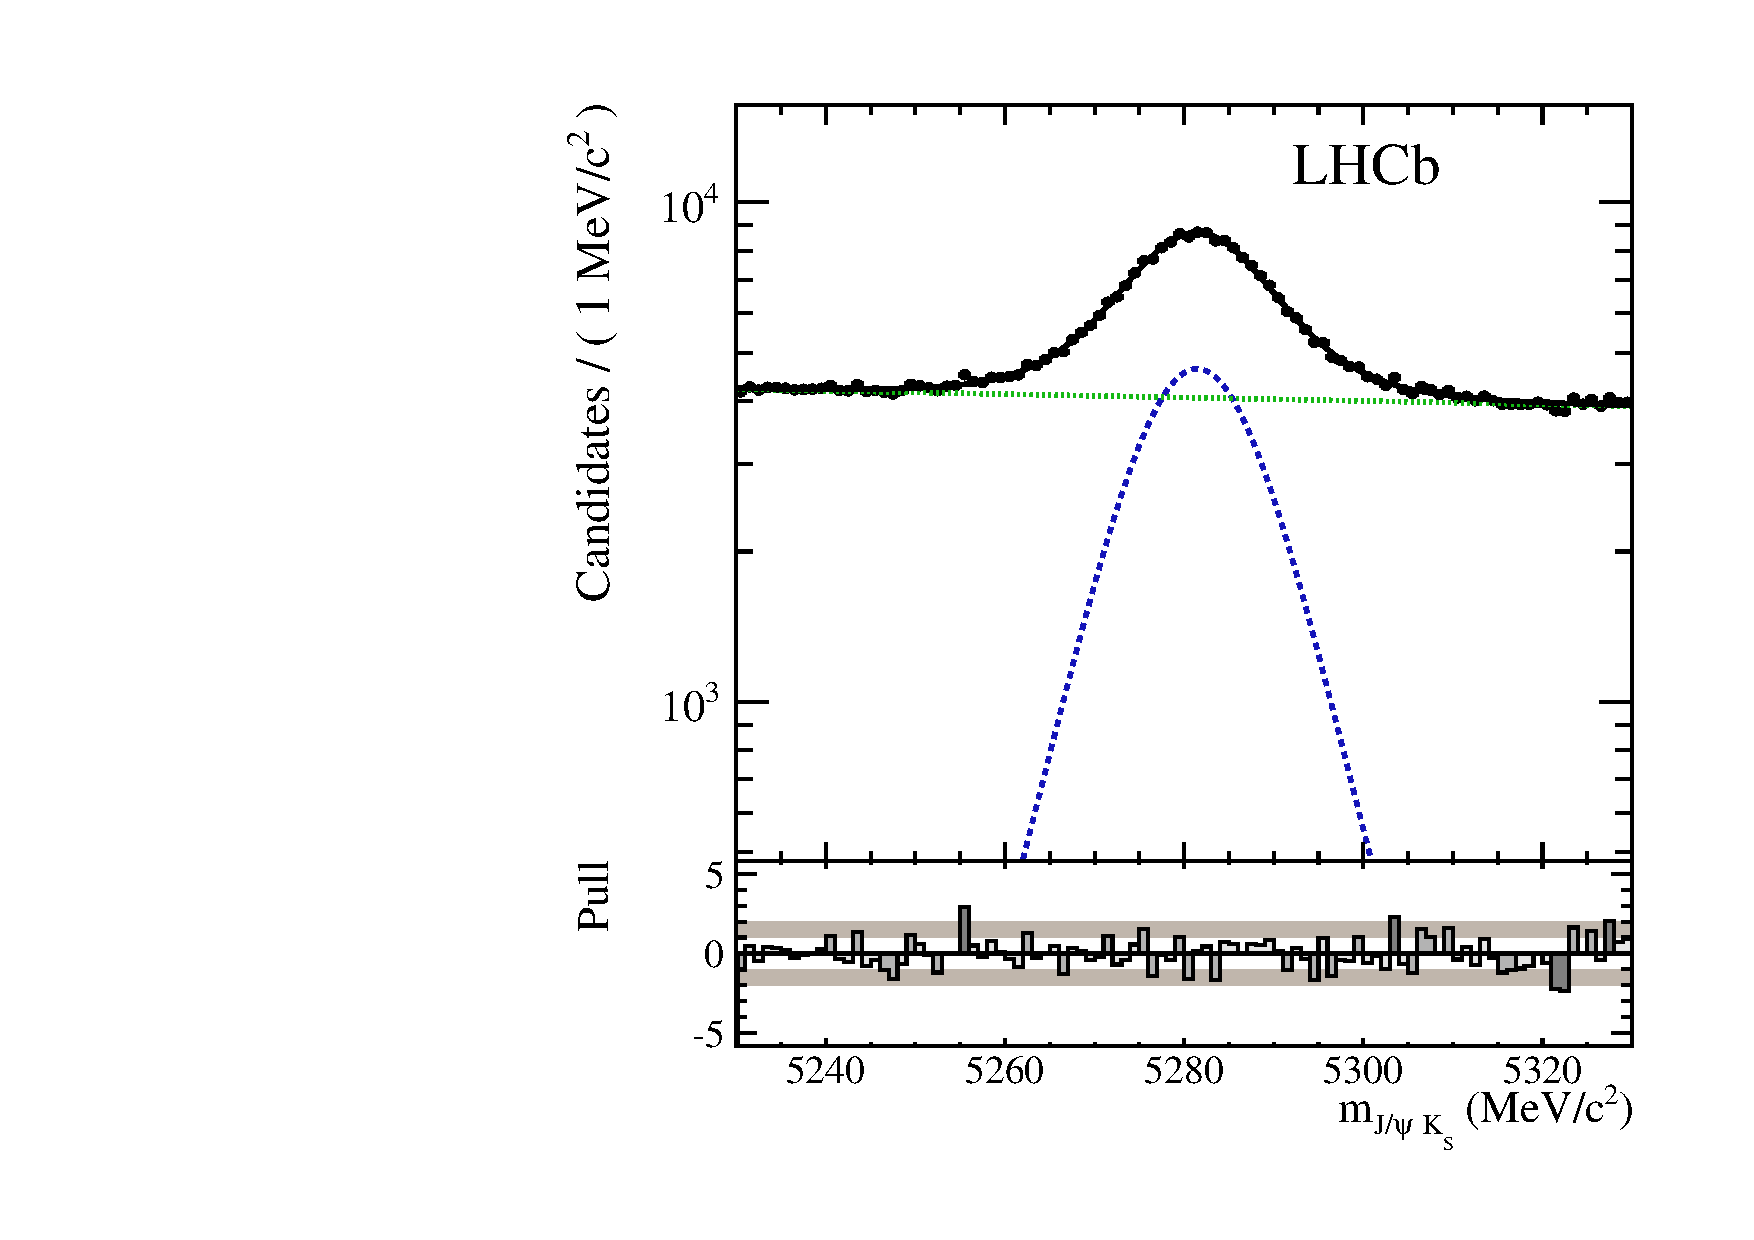
\includegraphics[width=0.49\textwidth]{private/content/measurement-of-sin2beta/figs/offline_splot_downstream.pdf}
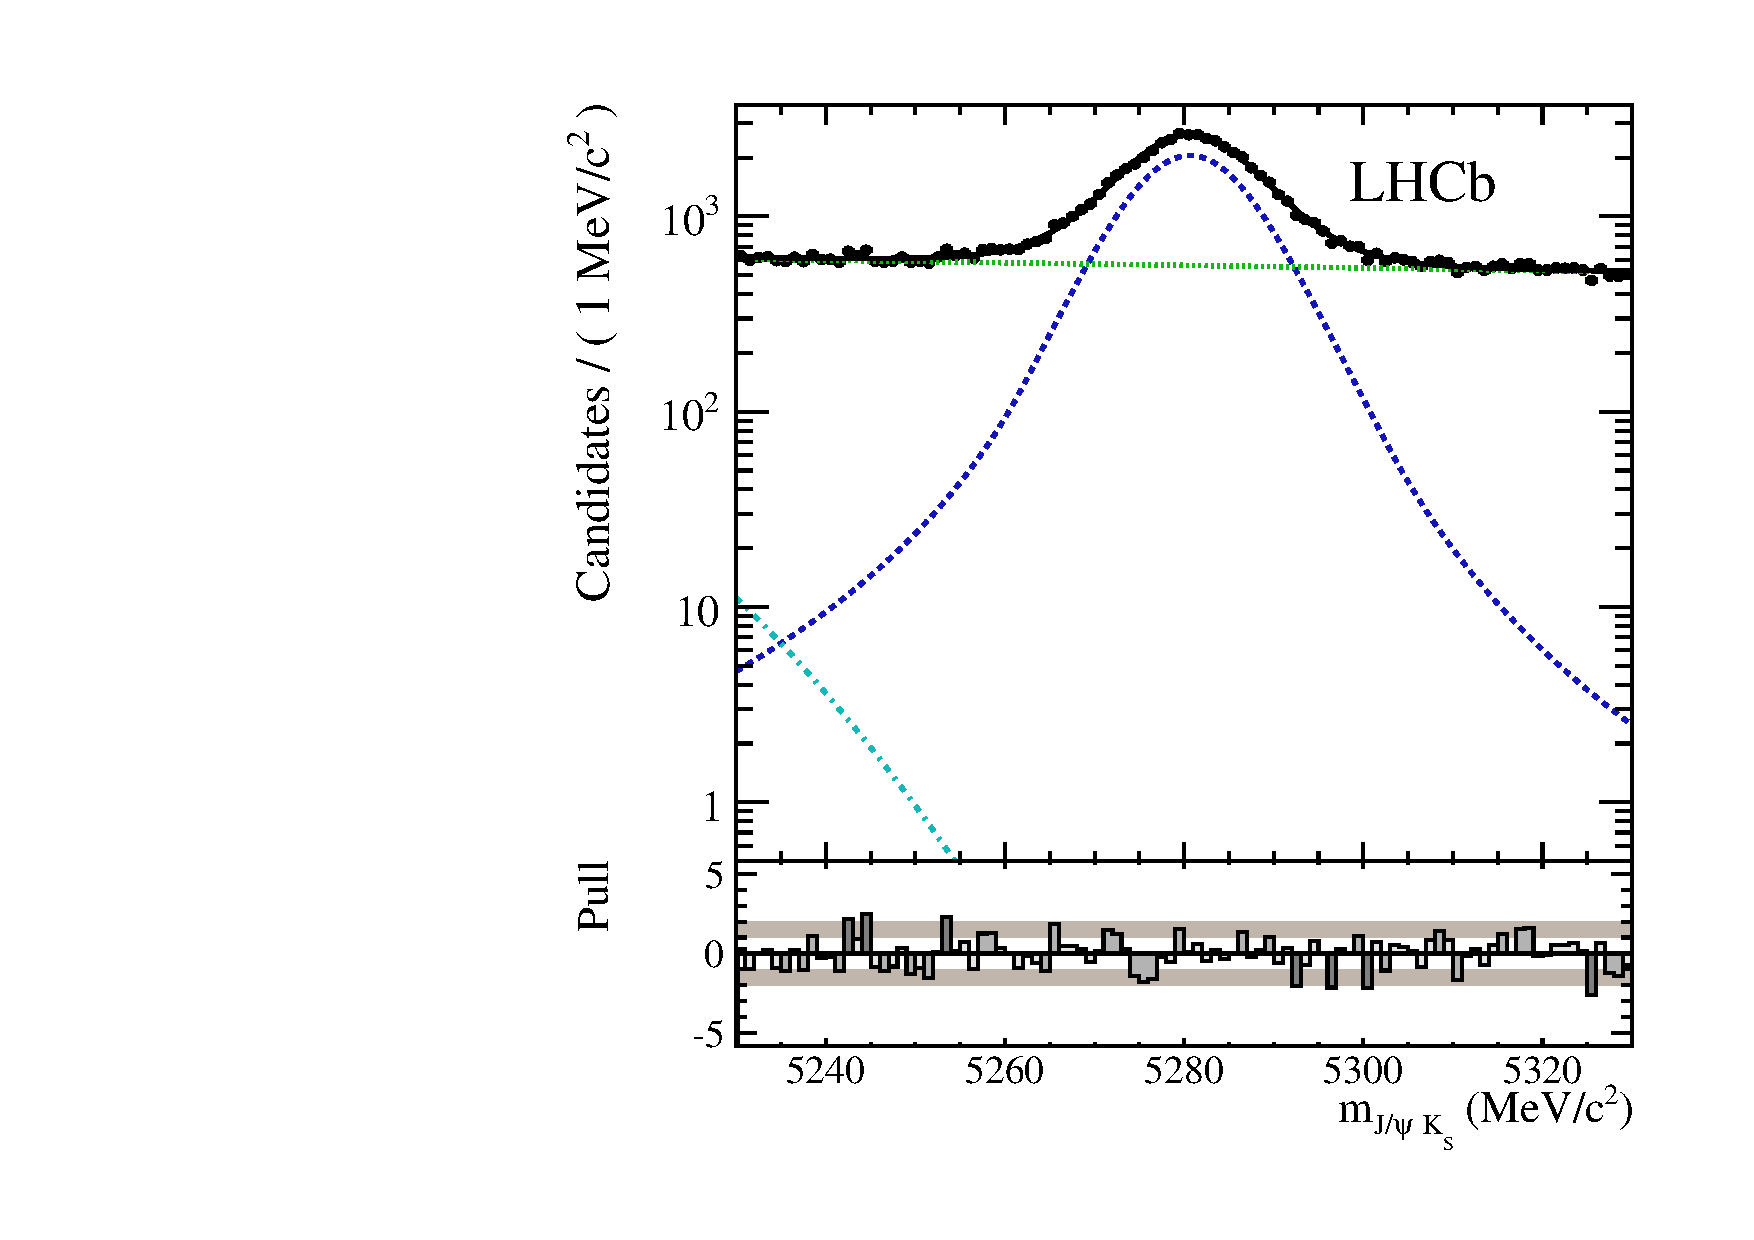
\includegraphics[width=0.49\textwidth]{private/content/measurement-of-sin2beta/figs/offline_splot_longtrack.pdf}
\label{fig:measurement_of_sin2beta:data_preparation:offline_selection:before}
\caption{Mass distribution of the combined 2011 and 2012 data set after
stripping (in logarithmic scale). Only the \PV with the smallest \IP \chisqndf
\wrt the $\Bd$ track is included and--- in case of multiple $\Bd$ candidates---a
random $\Bd$ candidate is chosen. The left plot shows the \catDD, the right one
the \catLL candidates. The solid black line is the projection of the fit \PDF,
the blue dashed line shows the signal, and the green dashed line shows the
background component. For the description of the \catLL candidates, the
additional $\BdToJpsiKstar$ component is depicted as dash-dotted turquoise line.
Below the mass distribution the pull distribution shows the difference of the
bin content and the \PDF value at the bin centre normalized by the error
estimate on the bin content.}
\end{figure}

%...............................................................................
\subsubsection{Sanity cuts}
\label{sec:measurement_of_sin2beta:data_preparation:offline_selection:sanity}

A set of sanity cuts (see
\cref{tab:measurement_of_sin2beta:data_preparation:offline_selection:sanity}) is
applied to remove outliers and ensure that all \DTF fits are converged. The
overall performance shows a signal efficiency of $\SI{99.29}{\percent}$
($\SI{99.75}{\percent}$) and a background rejection of $\SI{6.18}{\percent}$
($\SI{0.75}{\percent}$) in the \catDD (\catLL) sample.
%
\begin{table}
\centering
\caption{Offline selection sanity cuts.}
\label{tab:measurement_of_sin2beta:data_preparation:offline_selection:sanity}
\begin{tabular}{ll}
\toprule
\dtf $\sigma_m$                              & $<\SI[per-mode=symbol]{30}{\MeVcc}$\\
\dtfpv $\obsTimeError$                       & $<\SI[per-mode=symbol]{0.2}{\pico\second}$\\
$\vert z_{\acs*{PV}}\vert$                   & $<\SI{250}{\milli\meter}$\\
\Bd   $\chi_{\text{vtx}}^2/\ndf$             & $<10$\\
\jpsi $\chi_{\text{vtx}}^2/\ndf$             & $<16$\\
\KS   $\chi_{\text{vtx}}^2/\ndf$             & $<20$\\
\dtfpv $\mu$ $p_T$                           & $>\SI[per-mode=symbol]{500}{\MeVc}$\\
$\mu$ $\chi_{\text{track}}^2/\ndf$           & $<3$\\
$\mu$ \acs*{PID}                             & $>0$\\
\dtfpv $\pi\ p$                              & $>\SI[per-mode=symbol]{2000}{\MeVc}$\\
maximal $\pi$ $\chi_{\text{track}}^2/\ndf$   & $<3$\\
minimal $\pi$ \acs*{IP} $\chi^2/\ndf$        & $>4$\\
\multicolumn{2}{c}{\dtf fit and \dtfpv fit converged} \\
\bottomrule
\end{tabular}
\end{table}

%...............................................................................
\subsubsection{Ghost track probability cuts}
\label{sec:measurement_of_sin2beta:data_preparation:offline_selection:ghosts}

To reduce the amount of ghost tracks, a cut on each tracks ghost probability is
applied, as shown in
\cref{tab:measurement_of_sin2beta:data_preparation:offline_selection:ghosts}.
The overall signal efficiency yields $\SI{95.72}{\percent}$
($\SI{98.09}{\percent}$) with a background rejection of $\SI{26.38}{\percent}$
($\SI{23.36}{\percent}$) for the \catDD (\catLL) sample.
%
\begin{table}
\centering
\caption{Offline selection cuts on ghost track probabilities.}
\label{tab:measurement_of_sin2beta:data_preparation:offline_selection:ghosts}
\begin{tabular}{lll}
\toprule
& \catDD & \catLL\\
\midrule
$\mu$ ghost track probability & \multicolumn{2}{c}{$<0.2$}\\
$\pi$ ghost track probability & \multicolumn{2}{c}{$<0.3$}\\
\bottomrule
\end{tabular}
\end{table}

%...............................................................................
\subsubsection{Cuts on daughter masses and \Lambda mass veto}
\label{sec:measurement_of_sin2beta:data_preparation:offline_selection:daughters}

Background contributions due to particle mis-ID (\cf
\cref{sec:measurement_of_sin2beta:physic_backgrounds}) are reduced by employing
cuts on the invariant daughter masses are used as given in
\cref{tab:measurement_of_sin2beta:data_preparation:offline_selection:daughters}.
As long track candidates show a better mass resolution, different cuts are
applied depending on the candidates' track type. These cuts yield a signal
efficiency of $\SI{98.70}{\percent}$ ($\SI{98.92}{\percent}$) and a background
rejection of $\SI{27.53}{\percent}$ ($\SI{39.78}{\percent}$) in the \catDD
(\catLL) sample. The cuts correspond to roughly $8\sigma$ ($4\sigma$) for \catDD
(\catLL) $\KS$ candidates and around $5\sigma$ for the $\jpsi$ candidates.

To reduce pion-proton mis-ID all pion candidate pairs are combined, assigning
the proton mass hypothesis to either one of the pions and recalculating their
invariant mass. An additional requirement on the \proton-\pion \PID of
$\DLLppi<7$ ($<10$) is then applied to all candidates lying inside a
$\pm\SI{7}{\MeVcc}$ ($\pm\SI{5}{\MeVcc}$) region around the \Lambda mass
$M_\Lambda^{\text{\acs*{PDG}}} = \SI[per-mode=symbol]{1115.683}{\MeVcc}$ in the
\catDD (\catLL) sample. This \Lambda veto has a signal efficiency of
$\SI{99.32}{\percent}$ ($\SI{99.9}{\percent}$) and a background rejection of
$\SI{10.50}{\percent}$ ($\SI{2.53}{\percent}$) in the \catDD (\catLL) sample.
The cut efficiency on
\LbToJpsiLambda signal \MC is given in
\cref{sec:measurement_of_sin2beta:physic_backgrounds}.
%
\begin{table}
\centering
\caption{Offline selection cuts on the \jpsi and \KS candidates' invariant mass.
($M_{\jpsi}^{\text{\acs*{PDG}}}=\SI{3096.916}{\MeVcc}$,
$M_{\KS}^{\text{\acs*{PDG}}}=\SI{497.614}{\MeVcc}$)}
\label{tab:measurement_of_sin2beta:data_preparation:offline_selection:daughters}
\begin{tabular}{lll}
\toprule
& \multicolumn{1}{c}{\catDD} & \multicolumn{1}{c}{\catLL}\\
\midrule
$m_{\pi\pi}$ & $M_{\KS}^{\text{\acs*{PDG}}}\pm\SI[per-mode=symbol]{55}{\MeVcc}$ & $M_{\KS}^{\text{\acs*{PDG}}}\pm\SI[per-mode=symbol]{15}{\MeVcc}$\\
$m_{\mu\mu}$ & \multicolumn{2}{c}{$M_{\jpsi}^{\text{\acs*{PDG}}}\pm\SI[per-mode=symbol]{60}{\MeVcc}$}\\
\bottomrule
\end{tabular}
\end{table}

%...............................................................................
\subsubsection{DTF fit performance and \KS decay time significance cuts} 
\label{sec:measurement_of_sin2beta:data_preparation:offline_selection:dtf_and_dts}

Finally, cuts on the \dtf fit $\chisqndf<30$ and on the \KS decay time
significance (\wrt to the $\Bd$ decay vertex) of $t_{\KS}/\sigma_{t_{\KS}}>4$
from a \dtfpv fit are applied. These two cuts yield a signal efficiency of
$\SI{99.25}{\percent}$ ($\SI{97.61}{\percent}$) and a background rejection of
$\SI{33.68}{\percent}$ ($\SI{24.89}{\percent}$) for the \catDD (\catLL)
sample.

The fit range is limited to events within $\SI[per-mode=symbol]{0.3}{\pico\second}
<t<\SI[per-mode=symbol]{18.3}{\pico\second}$. Low decay time candidates are
neglected to suppress decay time acceptance effects and prompt background. The
number of candidates with decay times above the limit is negligible. This cut
yields a signal efficiency of $\SI{95.30}{\percent}$ ($\SI{94.86}{\percent}$)
and a background rejection of $\SI{12.77}{\percent}$ ($\SI{25.71}{\percent}$)
for the \catDD (\catLL) sample.

%...............................................................................
\subsubsection{Overall offline selection performance}
\label{sec:measurement_of_sin2beta:data_preparation:offline_selection:total}

\Cref{tab:measurement_of_sin2beta:data_preparation:offline_selection:total}
quotes the overall offline selection performance.
%
\begin{table}
\centering
\caption{Overall offline selection performance.}
\label{tab:measurement_of_sin2beta:data_preparation:offline_selection:total}
\begin{tabular}{lllll}
\toprule
& $\SigEff$ & $\BkgRej$ \\
\midrule
\catDD & $\SI{89.55}{\percent}$ & $\SI{67.61}{\percent}$\\
\catLL & $\SI{89.79}{\percent}$ & $\SI{70.60}{\percent}$\\
\bottomrule
\end{tabular}
\end{table}

% ------------------------------------------------------------------------------
\subsection{Multiple candidates}
\label{sec:measurement_of_sin2beta:data_preparation:multiple_candidates}

As in a typical \LHCb bunch crossing around $\num{2.5}$ visible
\acl{protonproton} collisions occur, the chances are high to find more than one
\PV per recorded event. Choosing the \PV with the smallest \DTF track \IP
\chisqndf \wrt the \Bd candidate is called \emph{best PV selection} in contrast
to a \emph{random PV selection}. Given the small \BdToJpsiKS branching ratio not
more than one signal event can be expected per event. Still, it is possible that
more than one candidate gets reconstructed. From those candidates either one can
be chosen by his \DTF track \IP \chisqndf\info{\wrt to a given PV?} (\emph{best
\Bd candidate selection}) or as well randomly (\emph{random \Bd candidate
selection}). Instead of consecutively selecting a \PV and \Bmeson candidate a
joint decision can be made. Each $(\text{\acs{PV}}, \Bd)$ pair can again be
chosen either based on the best fit quality or by random. The number of multiple
\acp{PV} and candidates is studied following Ref.~\cite{Koppenburg:1340942}.

After stripping selection around $\SI{2}{\percent}$ of the events contain more
than one \Bd candidate and $\SIrange[range-phrase = -, range-units = single]
{4}{5}{\percent}$ of all \Bmeson candidates are not unique in their event 
(\cf \cref{tab:measurement_of_sin2beta:data_preparation:multiple_candidates:after_stripping}).
%
\begin{table}
\centering
\caption{
Number of multiple \BdToJpsiKS candidates after stripping. The numbers in the
first row represent the fraction of \Bd candidates that are not \emph{unique} in
an event, \ie the event contains more than one candidate. The numbers in the
second row show the fraction of events with multiple \Bd candidates.
Additionally, a listing of the occurrence of events with different numbers of
multiple \Bd candidates is given. The last row shows the fraction of \Bd
candidates that need to be discarded in order to only get events with a single
\Bd candidate.}
\label{tab:measurement_of_sin2beta:data_preparation:multiple_candidates:after_stripping}
\begin{tabular}{lcccc}
\toprule
 & \multicolumn{2}{c}{2011} & \multicolumn{2}{c}{2012}\\
\midrule
fraction of multiple & \multicolumn{2}{c}{\multirow{2}[2]{*}{\SI{4.2}{\percent}}} & \multicolumn{2}{c}{\multirow{2}[2]{*}{\SI{4.9}{\percent}}}\\
\Bd candidates & & & & \\
\midrule
fraction of events with & \multicolumn{2}{c}{\multirow{2}[2]{*}{\SI{2.1}{\percent}}} & \multicolumn{2}{c}{\multirow{2}[2]{*}{\SI{2.4}{\percent}}}\\
 multiple \Bd candidates & & & & \\  
\cmidrule(r){2-5}
 & \#\Bd cands & \#events & \#\Bd cands & \#events\\
\cmidrule(r){2-5}
 & 1 & 575780 & 1 & 1482895\\
 & 2 & 11997  & 2 & 35921\\
 & 3 & 382    & 3 & 1223\\
 & 4 & 50     & 4 & 194\\
 & 5 & 4      & 5 & 9\\
 & 6 & 1      & 6 & 9\\
 & 7 & 0      & 7 & 1\\
\midrule
fraction of \Bd candidates & \multicolumn{2}{c}{\multirow{2}[2]{*}{\SI{2.2}{\percent}}} & \multicolumn{2}{c}{\multirow{2}[2]{*}{\SI{2.5}{\percent}}}\\
to discard & & & & \\
\bottomrule
\end{tabular}
\end{table}
%
After stripping and subsequent offline selection roughly $\SI{0.3}{\percent}$ of
events contain multiple \Bd candidates while in $\SI{6}{\percent}$ of the events
more than one \PV is found. 
\Cref{tab:measurement_of_sin2beta:data_preparation:multiple_candidates:after_selection} 
presents the detailed numbers for multiple \PV and \Bd candidates after
stripping and offline selection. Of the remaining (\acs{PV},\Bd) pairs one is
chosen randomly.
%
\begin{table}
\centering
\caption{ 
Number of multiple candidates after stripping and selection. The numbers in the
first row represent the fraction of (\PV,\Bd) candidate pairs that are not
unique in an event. The numbers in the second row show the fraction of events
with multiple (\PV,\Bd) candidate pairs.  The third row includes the numbers of
event with multiple \Bd candidates. Additionally, a listing of the occurrence of
events with different numbers of multiple \Bd candidates is given. After that,
the number of \Bd candidates to discard is given. In the fourth row the number
of events containing multiple \acp{PV} is listed together with the detailed
description of the frequency of multiple \acp{PV} per event. The last row shows
the fraction of (\PV,\Bd) candidate pairs that need to be discarded in order to
only keep one (\PV,\Bd) candidate per event. }
\label{tab:measurement_of_sin2beta:data_preparation:multiple_candidates:after_selection}
\begin{tabular}{lcccc}
\toprule
 & \multicolumn{2}{c}{2011} & \multicolumn{2}{c}{2012}\\
\midrule
fraction of multiple & \multicolumn{2}{c}{\multirow{2}[2]{*}{\SI{12.5}{\percent}}} & \multicolumn{2}{c}{\multirow{2}[2]{*}{\SI{12.8}{\percent}}}\\
candidates & & & & \\
\midrule
fraction of events with& \multicolumn{2}{c}{\multirow{2}[2]{*}{\SI{6.0}{\percent}}} & \multicolumn{2}{c}{\multirow{2}[2]{*}{\SI{6.1}{\percent}}}\\
multiple (\acs{PV},\Bd) candidates & & & & \\  
\midrule
fraction of events with & \multicolumn{2}{c}{\multirow{2}[2]{*}{\SI{0.3}{\percent}}} & \multicolumn{2}{c}{\multirow{2}[2]{*}{\SI{0.4}{\percent}}}\\
multiple \Bd candidates & & & & \\  
\cmidrule(r){2-5}
 & \#\Bd cands & \#events & \#\Bd cands & \#events\\
\cmidrule(r){2-5}
 & 1 & 74065 & 1 & 165915\\
 & 2 & 253   & 2 & 635\\
 & 3 & 0     & 3 & 3\\
 \midrule
fraction of \Bd candidates & \multicolumn{2}{c}{\multirow{2}[2]{*}{\SI{0.3}{\percent}}} & \multicolumn{2}{c}{\multirow{2}[2]{*}{\SI{0.4}{\percent}}}\\
to discard & & & & \\
 \midrule
fraction of events & \multicolumn{2}{c}{\multirow{2}[2]{*}{\SI{5.7}{\percent}}} & \multicolumn{2}{c}{\multirow{2}[2]{*}{\SI{5.8}{\percent}}}\\
with multiple \acp{PV} & & & & \\  
\cmidrule(r){2-5}
 & \#\acsp{PV} & \#events & \#\acsp{PV} & \#events\\
\cmidrule(r){2-5}
 & 1 & 69755 & 1 & 156211\\
 & 2 & 4279  & 2 & 9583\\
 & 3 & 265   & 3 & 692\\
 & 4 & 19    & 4 & 58\\
 & 5 & 0     & 5 & 9\\
\midrule
fraction of (\acs{PV},\Bd) candidate & \multicolumn{2}{c}{\multirow{2}[2]{*}{\SI{6.5}{\percent}}} & \multicolumn{2}{c}{\multirow{2}[2]{*}{\SI{6.6}{\percent}}}\\
pairs to discard & & & & \\
\bottomrule
\end{tabular}
\end{table}

% ------------------------------------------------------------------------------
\subsection{\acs{MC} and data samples}
\label{sec:measurement_of_sin2beta:data_preparation:datasamples}

\redo{Rewrite MC and data samples}

Over the course of the described measurement several datasets are utilised such
as recorded data from the \LHCb experiment as well as simulated data.

All candidates in the nominal dataset finally used for the fit to estimate the
\CP observables \SJpsiKS and \CJpsiKS pass the given trigger configuration, the
detached stripping selection, and the described offline selection leaving
$\num{114000}$ signal candidates. The analysis only makes use of $\num{42000}$
tagged signal candidates.
\Cref{tab:measurement_of_sin2beta:data_preparation:datasamples:numbers} lists
the numbers of tagged signal candidates split into subsamples of tagger,
trigger, track type, and year of data-taking.
%
\begin{table}
\centering
\caption{Number of tagged signal candidates split into categories of tagger, 
trigger, track type, and year of data-taking. All numbers rounded.}
\label{tab:measurement_of_sin2beta:data_preparation:datasamples:numbers}
\begin{tabular}{c|c|c|c|c|c|c|c|c|c|c}
\toprule
\multicolumn{1}{c}{} & \multicolumn{5}{c}{DD} & \multicolumn{5}{c}{LL}\\
\midrule
\multirow{6}[6]{*}{\catOO} & \multirow{2}[2]{*}{\catOS} & \catAU & \num{5134} & \multirow{2}[2]{*}{\num{5991}} & \multirow{6}[6]{*}{\num{9423}} & \multirow{2}[2]{*}{\catOS} & \catAU & \num{2263} & \multirow{2}[2]{*}{\num{2597}} & \multirow{6}[6]{*}{\num{3799}}\\
\cmidrule(r){3-4}\cmidrule(r){8-9}
& & \catEB & \num{857} & & & & \catEB & \num{334} & & \\
\cmidrule(r){2-5}\cmidrule(r){7-10}
 & \multirow{2}[2]{*}{\catSS} & \catAU & \num{2028} & \multirow{2}[2]{*}{\num{2352}} & & \multirow{2}[2]{*}{\catSS} & \catAU & \num{744} & \multirow{2}[2]{*}{\num{834}} & \\
 \cmidrule(r){3-4}\cmidrule(r){8-9}
 & & \catEB & \num{324} & & & & \catEB & \num{90} & & \\
\cmidrule(r){2-5}\cmidrule(r){7-10}
 & \multirow{2}[2]{*}{BS} & \catAU & \num{941} & \multirow{2}[2]{*}{\num{1080}} & & \multirow{2}[2]{*}{BS} & \catAU & \num{321} & \multirow{2}[2]{*}{\num{368}} & \\
 \cmidrule(r){3-4}\cmidrule(r){8-9}
 & & \catEB & \num{139} & & & & \catEB & \num{47} & & \\
 \midrule
\multirow{6}[6]{*}{\catOT} & \multirow{2}[2]{*}{\catOS} & \catAU & \num{10378} & \multirow{2}[2]{*}{\num{12567}} & \multirow{6}[6]{*}{\num{20160}} & \multirow{2}[2]{*}{\catOS} & \catAU & \num{4599} & \multirow{2}[2]{*}{\num{5571}} & \multirow{6}[6]{*}{\num{8178}}\\
\cmidrule(r){3-4}\cmidrule(r){8-9}
& & \catEB & \num{2189} & & & & \catEB & \num{972} & & \\
\cmidrule(r){2-5}\cmidrule(r){7-10}
 & \multirow{2}[2]{*}{\catSS} & \catAU & \num{4247} & \multirow{2}[2]{*}{\num{5226}} & & \multirow{2}[2]{*}{\catSS} & \catAU & \num{1550} & \multirow{2}[2]{*}{\num{1831}} & \\
 \cmidrule(r){3-4}\cmidrule(r){8-9}
 & & \catEB & \num{979} & & & & \catEB & \num{281} & & \\
\cmidrule(r){2-5}\cmidrule(r){7-10}
 & \multirow{2}[2]{*}{BS} & \catAU & \num{1963} & \multirow{2}[2]{*}{\num{2367}} & & \multirow{2}[2]{*}{BS} & \catAU & \num{658} & \multirow{2}[2]{*}{\num{776}} & \\
 \cmidrule(r){3-4}\cmidrule(r){8-9}
 & & \catEB & \num{404} & & & & \catEB & \num{118} & & \\
\bottomrule
\end{tabular}
\label{tab:data_preparation:nominal}
\end{table}
%
\begin{figure}[!htb]
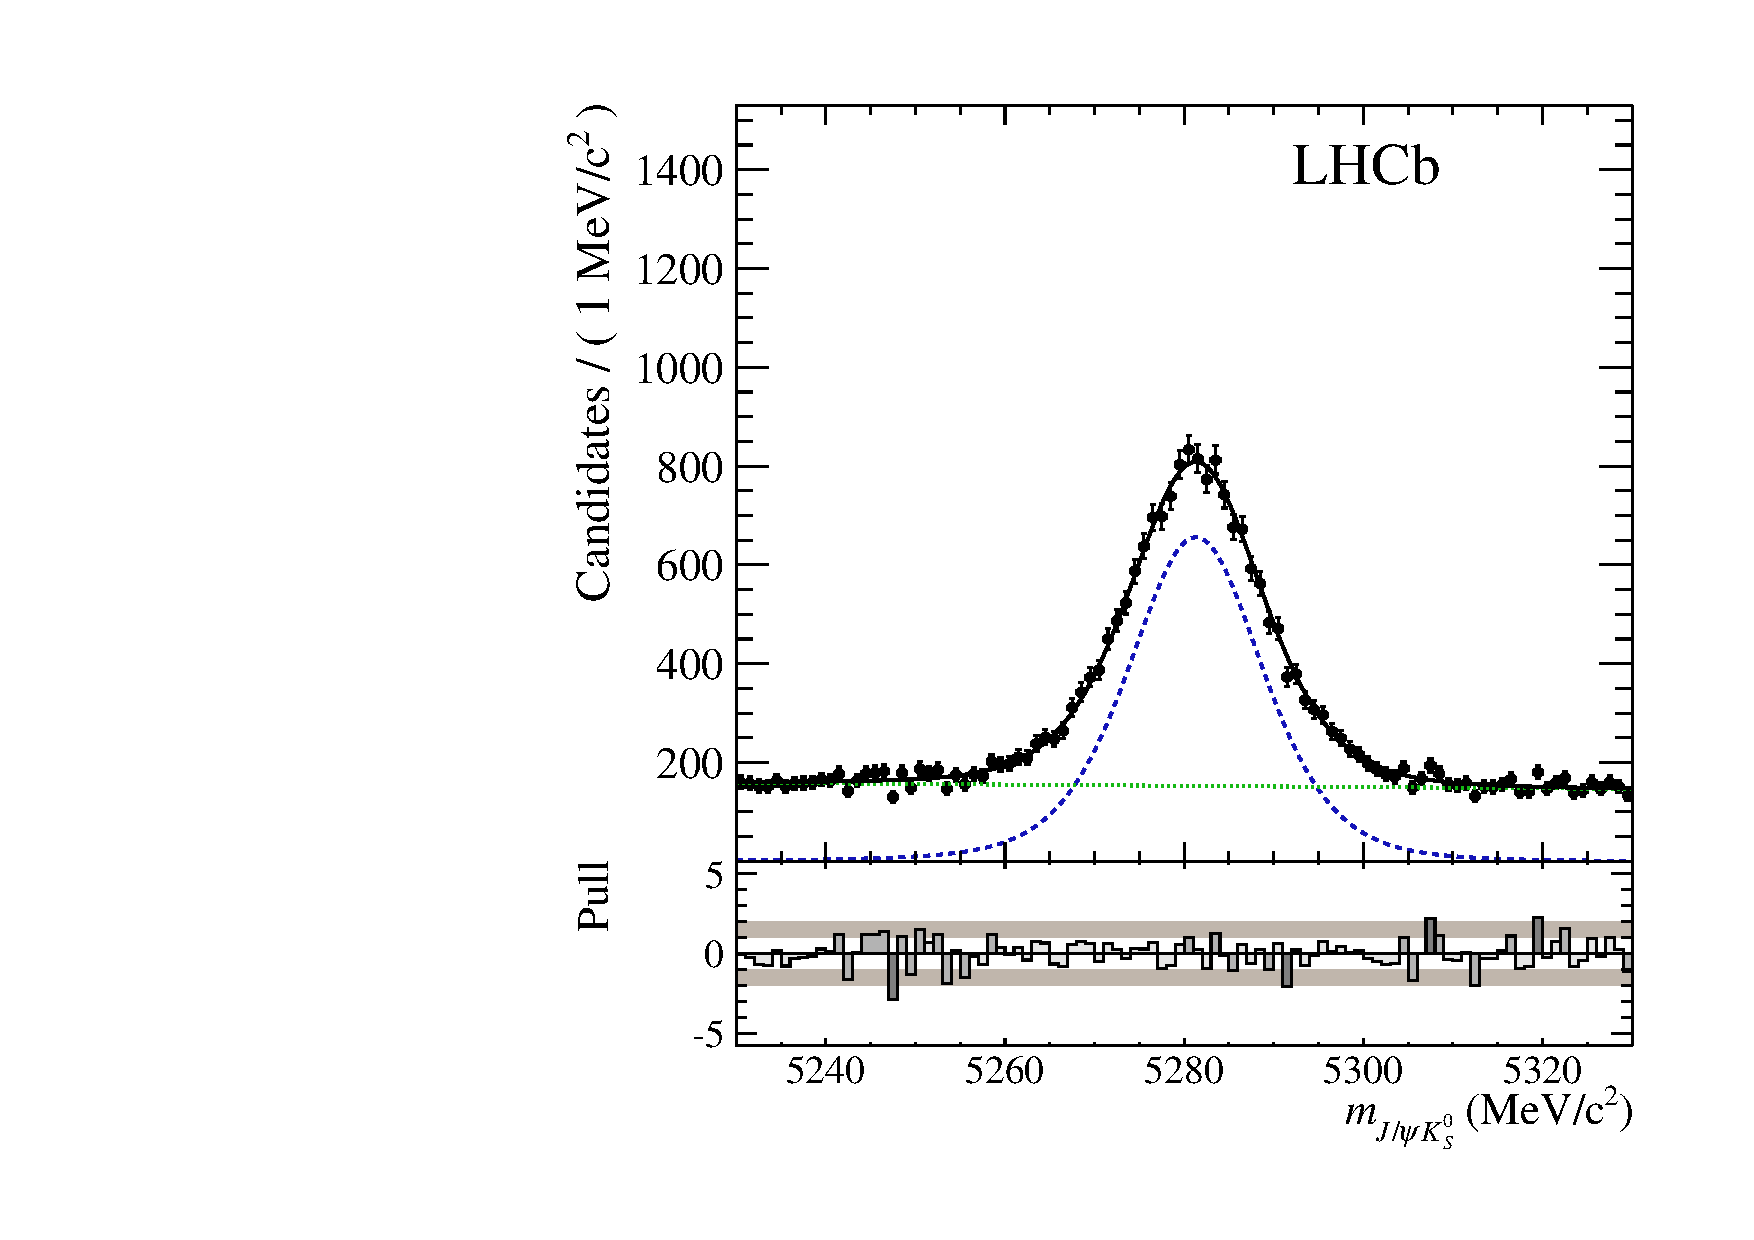
\includegraphics[width=0.49\textwidth]{private/content/measurement-of-sin2beta/figs/mass_11.pdf}
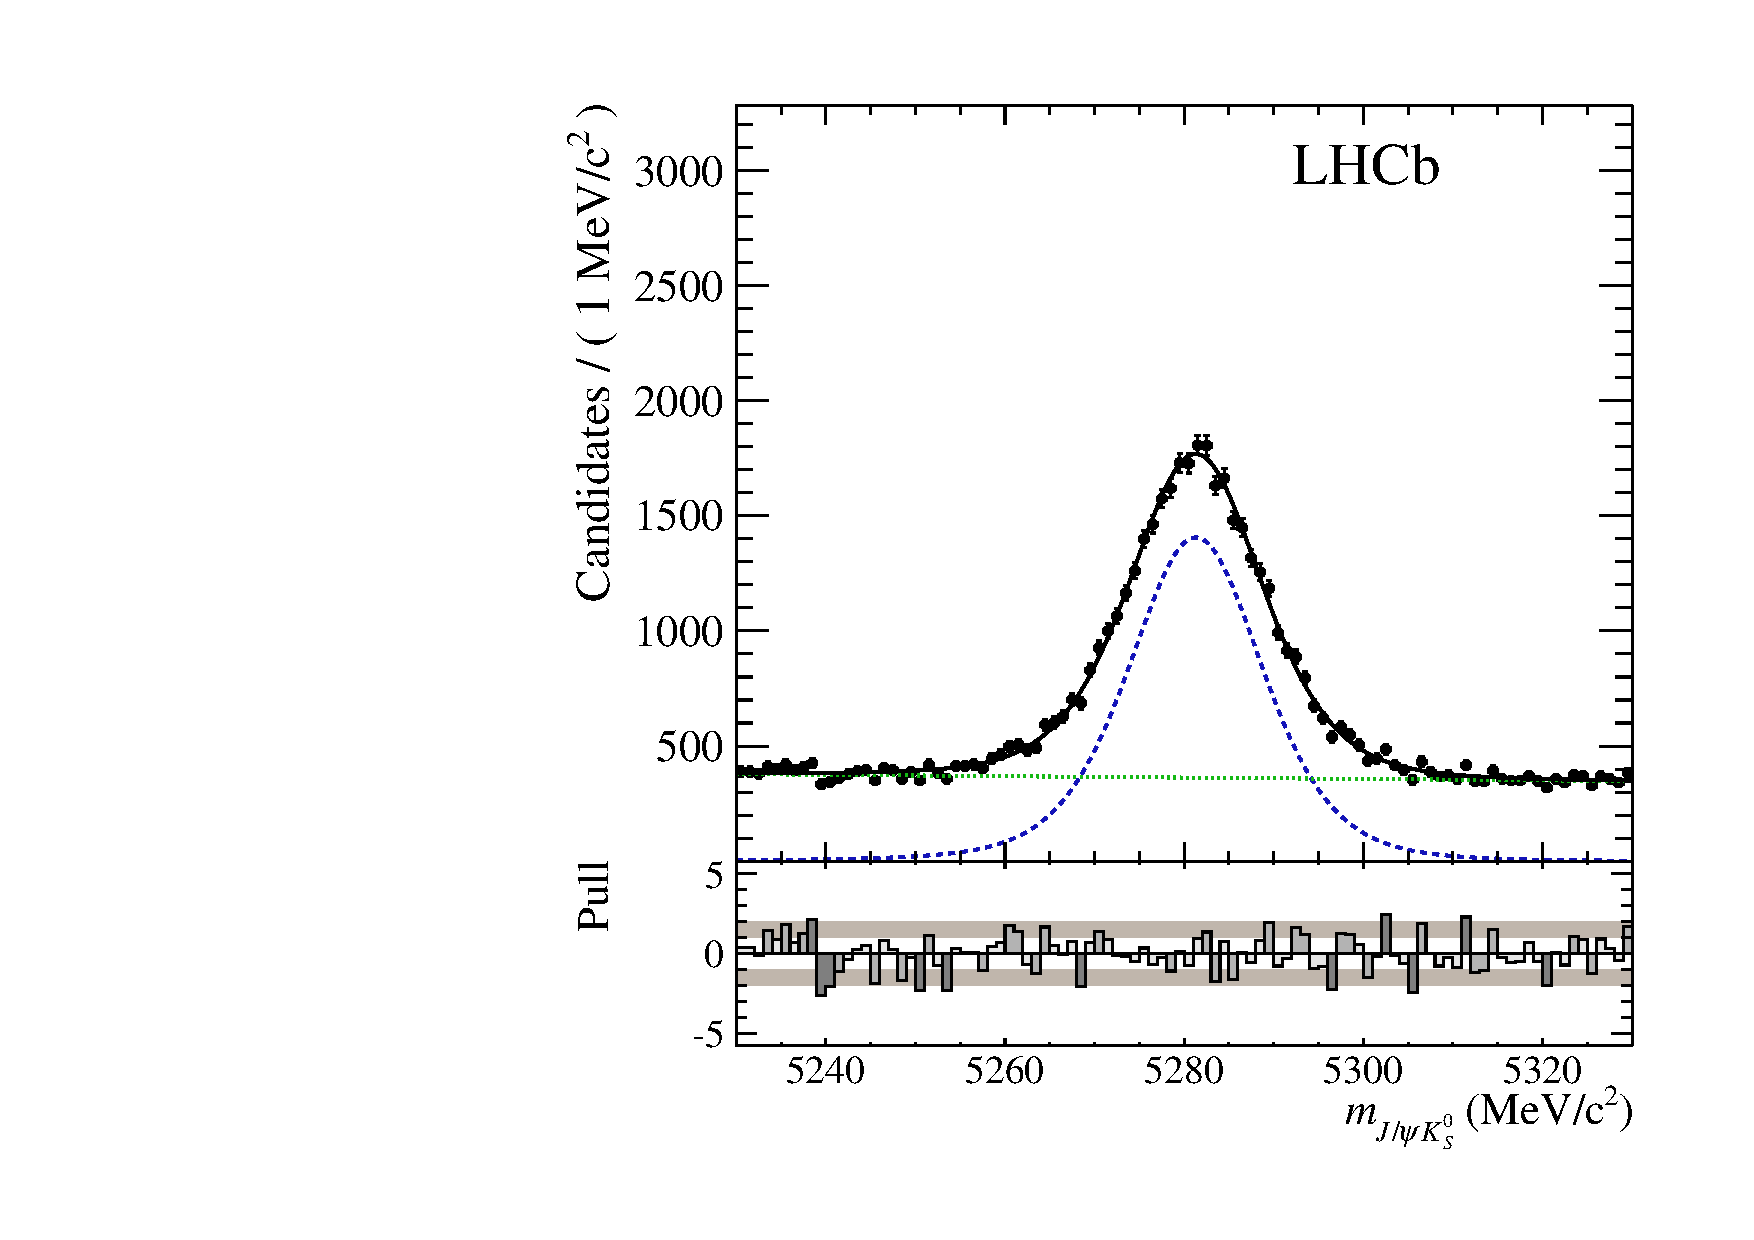
\includegraphics[width=0.49\textwidth]{private/content/measurement-of-sin2beta/figs/mass_12.pdf}
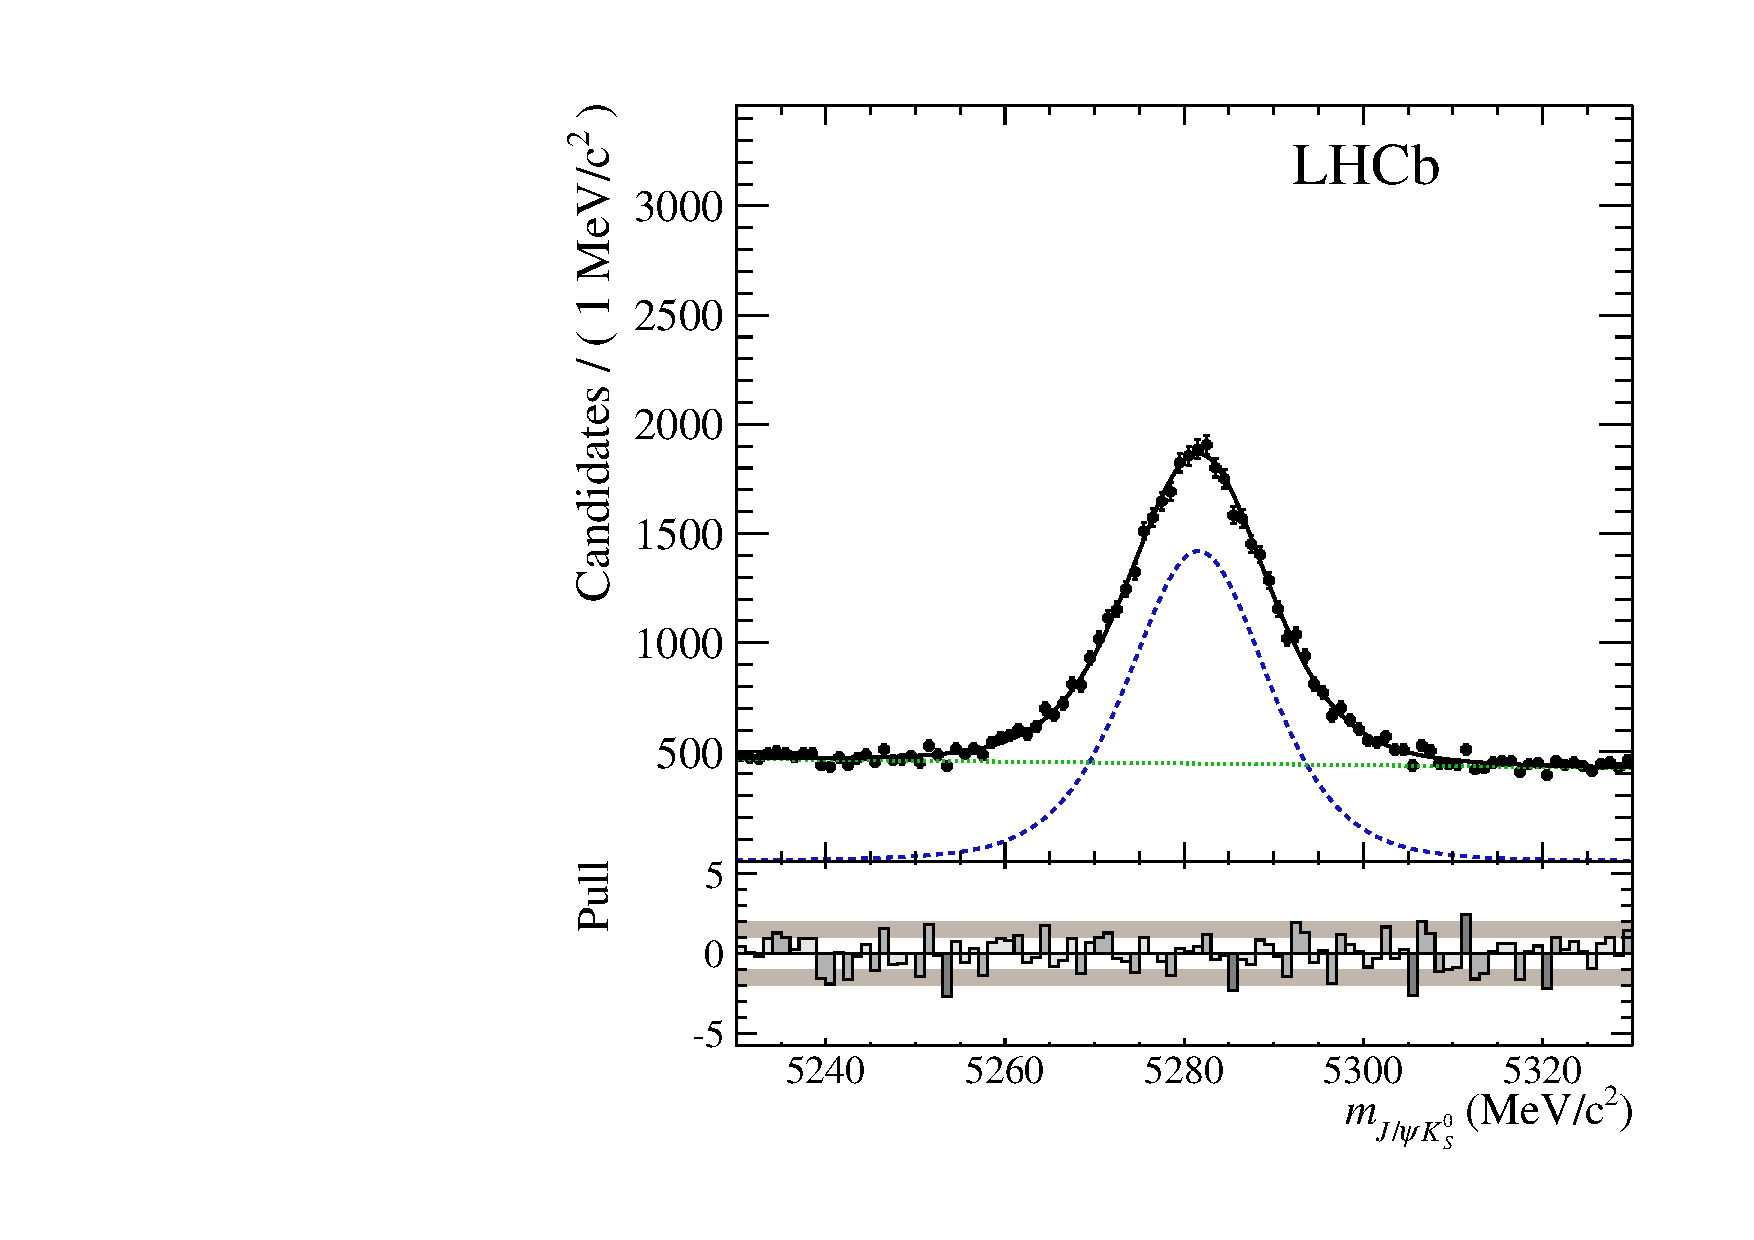
\includegraphics[width=0.49\textwidth]{private/content/measurement-of-sin2beta/figs/mass_DD.pdf}
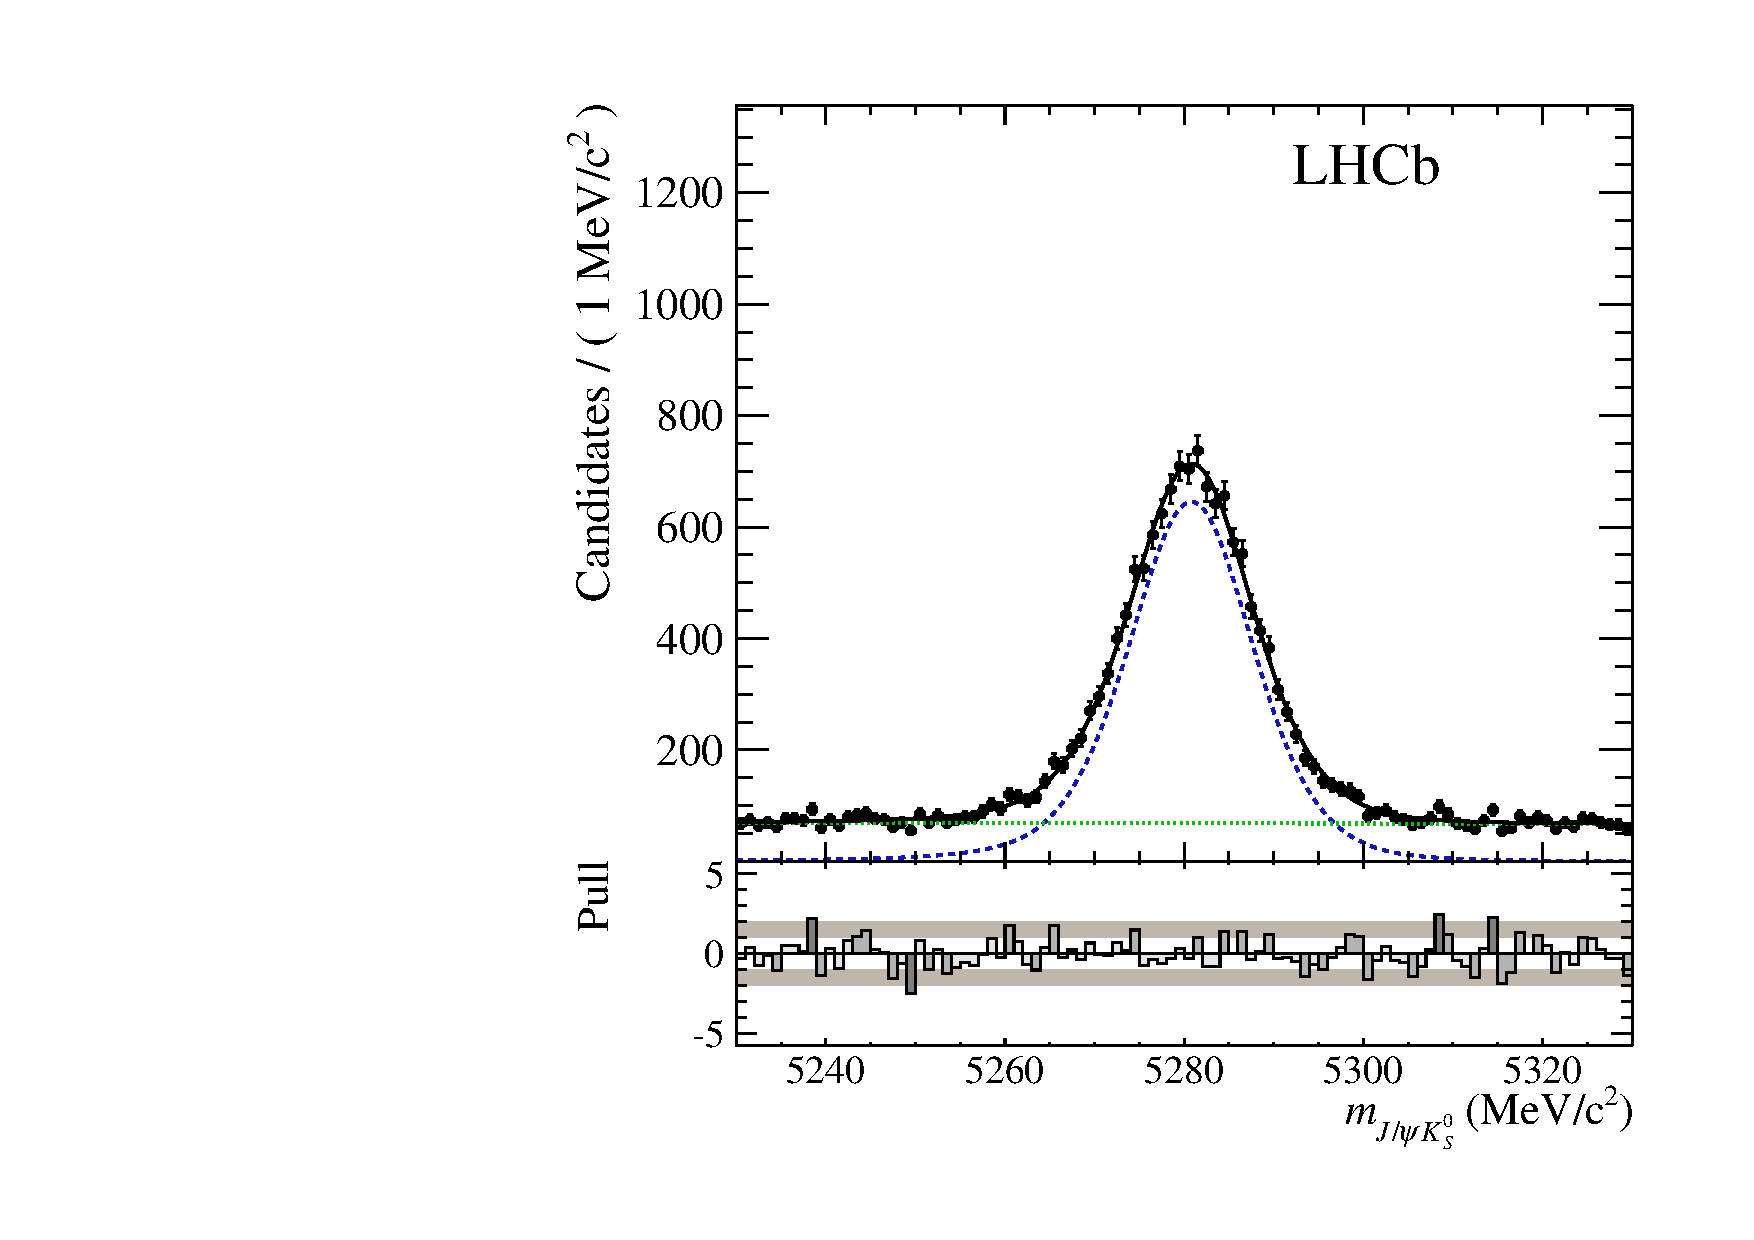
\includegraphics[width=0.49\textwidth]{private/content/measurement-of-sin2beta/figs/mass_LL.pdf}
\label{fig:measurement_of_sin2beta:data_preparation:datasamples:split}
\caption{Mass distribution of the nominal data set, split into year of
data-taking and into $\KS$ track type. Top row: on the left \catOO, on the right
\catOT. Bottom row: on the left \catDD, on the right \catLL. The solid black
line shows the fit projection of the nominal mass \ac{PDF} (\cf
\cref{sec:measurement_of_sin2beta:likelihood_fit:model:mass}). The blue dashed
line shows the signal, the green dashed line the background component.}
\end{figure}
%
\begin{figure}
\centering
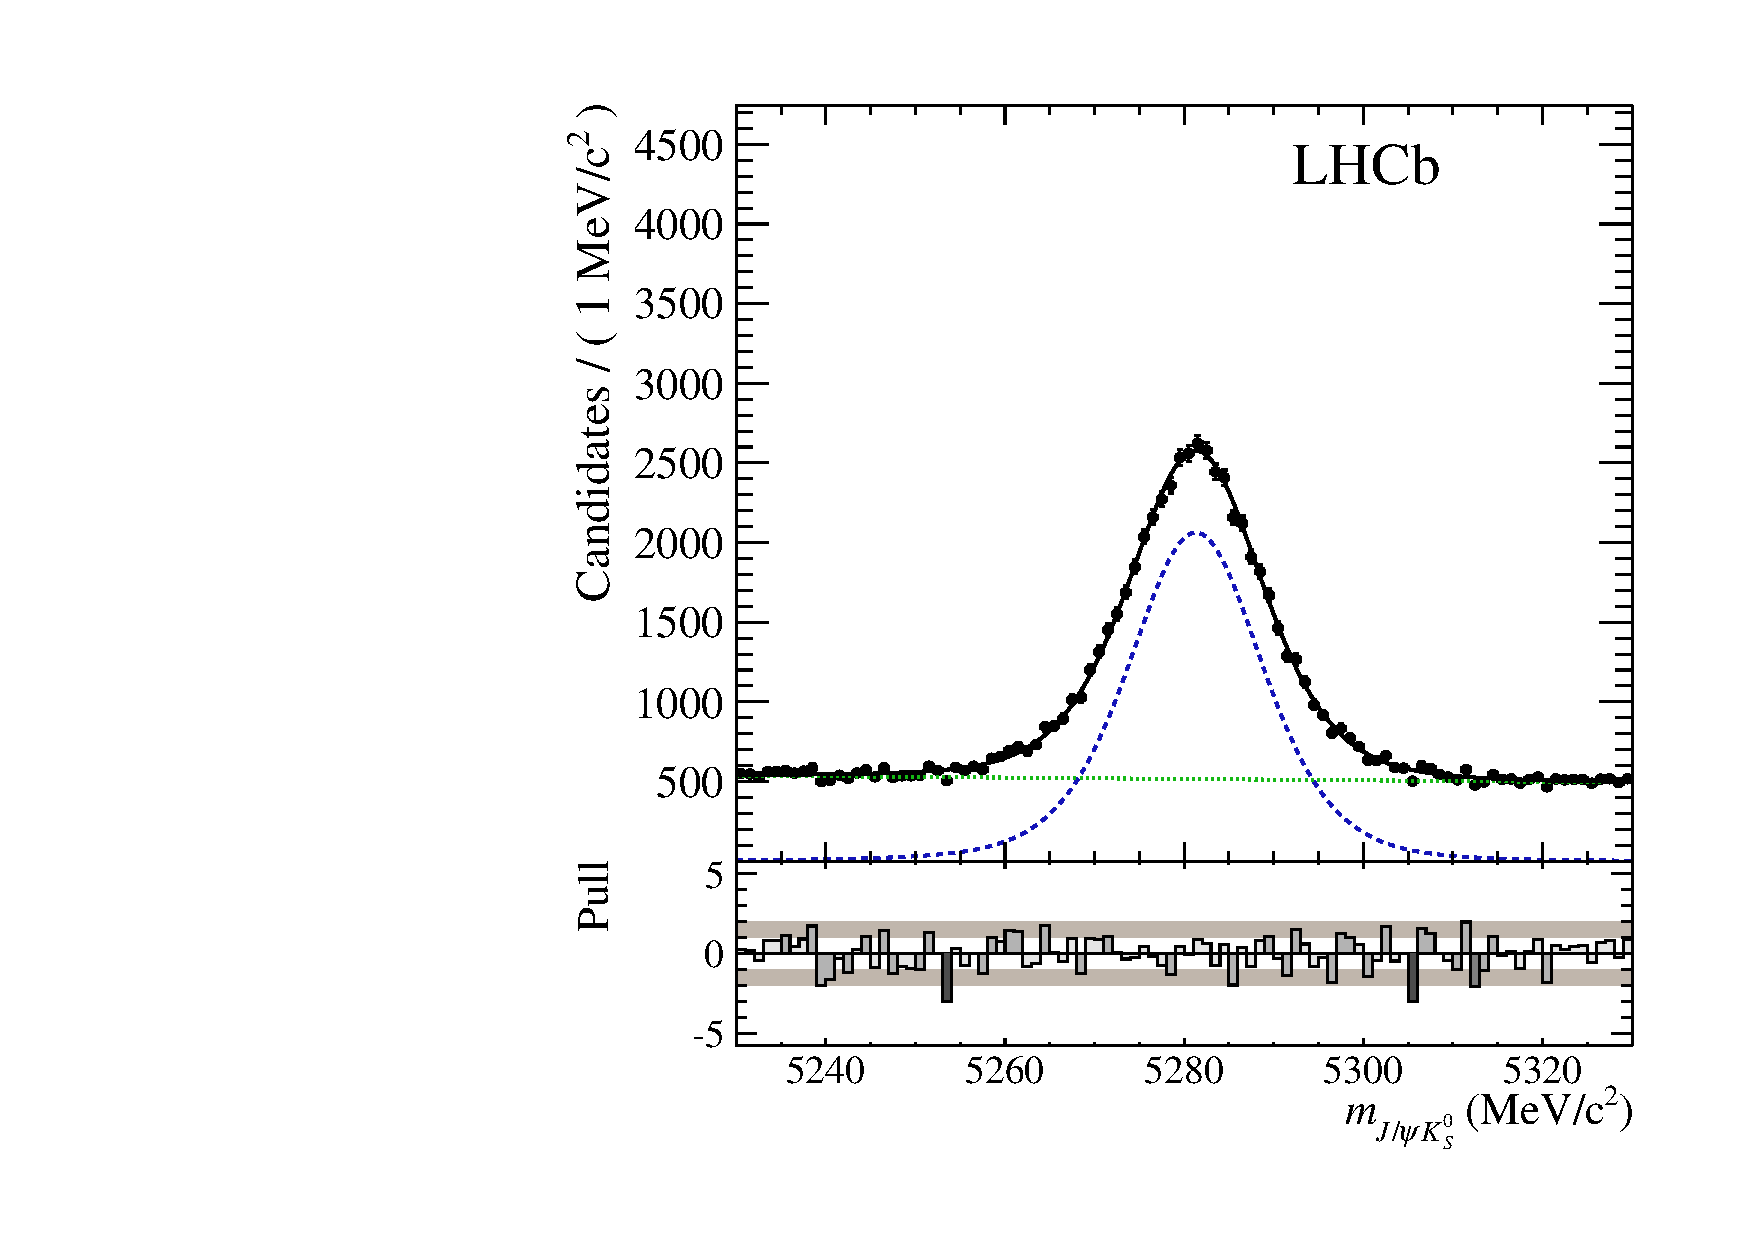
\includegraphics[width=0.8\textwidth]{private/content/measurement-of-sin2beta/figs/mass.pdf}
\label{fig:measurement_of_sin2beta:data_preparation:datasamples:combined}
\caption{Combined mass distribution of the nominal data set for all different
categories. The solid black line shows the fit projection of the nominal mass
\ac{PDF} (\cf \cref{sec:measurement_of_sin2beta:likelihood_fit:model:mass}). The
blue dashed line shows the signal, the green dashed line the background
component.}
\end{figure}

%...............................................................................
\subsubsection{\MC datasets}
\label{sec:measurement_of_sin2beta:data_preparation:datasamples:mc}

The \acf{MC} samples are produced using \PythiaSix and \PythiaEight in the
generation step. An equal amount of events is generated using each generator
version and also for both possible magnet polarities called \emph{up} and
\emph{down}. Also different samples are produced for \catOO and \catOT running
conditions. Heavy particles from generated \protonproton collisions are decayed
using \EvtGen and the particle interactions with the \LHCb detector material is
handled by \GeantFour. The \EvtGen physics model is set to \Verb=SSD_CP= with
parameters as summarised in
\cref{tab:measurement_of_sin2beta:data_preparation:datasamples:mc:decfile}. The
detector response is simulated using \Boole. The \LHCb trigger software \Moore,
the reconstruction based on \Brunel and the stripping selection using \DaVinci
treat simulated and recorded data in the same manner.
\info{Quote software versions? FT package?}
%
\begin{table}
\centering
\caption{Physics parameters used in the simulation.}
\label{tab:measurement_of_sin2beta:data_preparation:datasamples:mc:decfile}
\begin{tabular}{ll}
\toprule
Parameter                            & Generation value \\
\midrule
$\DMd$                               & \SI{0.502e12}{(\planckbar\per\second)} \\
$\frac{\DG}{\Gamma}$                 & \num{0} \\
$\left\vert\frac{q}{p}\right\vert$   & \num{1} \\
$\arg(\frac{q}{p})$                  & \num{-0.775} \\
$\vert A_f \vert$                    & \num{1} \\
$\arg(A_f)$                          & \num{0} \\
$\left\vert A_{\bar{f}} \right\vert$ & \num{-1}  \\
$\arg(A_{\bar{f}})$                  & \num{0} \\
$\tau$                               & \SI{1.519068}{\pico\second}\\
\bottomrule
\end{tabular}
\end{table}
%
Studies to check for possible background contributions from partly reconstructed
decays or decays with mis-identified particles (outlined in
\cref{sec:measurement_of_sin2beta:physic_backgrounds}) require several inclusive
and signal \MC samples using the same \replace{conditions}{by better wording} as for the nominal \MC data
set. \Cref{tab:measurement_of_sin2beta:data_preparation:datasamples:mc:samples}
shows the used \MC data sets and gives the number of generated events.
%
\begin{table}
\centering
\caption{Inclusive and signal MC data sets used in this analysis, with the
generated number of events and if possible an estimate on the corresponding
integrated luminosity.}
\label{tab:measurement_of_sin2beta:data_preparation:datasamples:mc:samples}
\begin{tabular}{lll}
\toprule
\acs{MC} name & \# events & int.\ lumi.\ $[\si{\per\fb}]$ \\ 
\midrule
inclJpsi    & \SI{60}{M} & -             \\
Bd2JpsiX    & \SI{20}{M} & -             \\
Bu2JpsiX    & \SI{20}{M} & -             \\
Bs2JpsiX    & \SI{20}{M} & -             \\
Bd2JpsiKst  & \SI{4}{M}  & $\approx 1.6$ \\
Lb2JpsiL    & \SI{3}{M}  & $\approx 15$  \\
\bottomrule
\end{tabular}
\end{table}

\FloatBarrier

% %%%%%%%%%%%%%%%%%%%%%%%%%%%%%%%%%%%%%%%%%%%%%%%%%%%%%%%%%%%%%%%%%%%%%%%%%%%%%%
%!TEX root = ../../common/main.tex

\chapter{Flavour Tagging}
\label{ch:flavour_tagging}

The time-dependent measurement of the $\CP$ asymmetry $\CPAsymmetry$ in the
decay of $\Bd$ and $\Bdbar$ mesons into the $\CP$ eigenstate $\Jpsi\KS$ requires
the knowledge of the \Bmeson flavour at production, \ie weather it contained
a $\bquark$ or a $\bquarkbar$. The method and algorithms used to infer this
information from all available event properties are named \enquote{flavour
tagging}.

Each tagging algorithm provides a tag $\tagdecision$ and a probability estimate
$\mistagestimate$ that the assigned tag is wrong, also called \enquote{mistag}
estimate. The tag is $\tagdecision=+1$ for an initial $\Bd$, $\tagdecision=-1$
for an initial $\Bdbar$, and $\tagdecision=0$ if the tagging algorithms were not
able to determine a decision. The mistag estimate interval is given by
$[0,0.5[$, where mistags $\mistagestimate^{\prime}>0.5$ are evaluated as
$\mistagestimate = 1 - \mistagestimate^{\prime}$ and the corresponding tag's
sign is reversed. If the algorithm is not able to determine a decision, the
mistag is set $\mistagestimate=0.5$.

The performance of the flavour tagging algorithms can be assigned using control
samples of \Bmesons whose final state determines the $\B$ flavour at decay
time (\ie are \enquote{flavour-specific}), \eg $\BuToJpsiK$ where the charge of
the kaon allows to infer the charge of the $\B$.

Given the numbers of all right tagged $\B$ candidates $\NRtagged$, all wrong
tagged candidates $\NWtagged$, and all \enquote{untagged} candidates
$\NUtagged$, the \enquote{tagging efficiency} $\tageff$ can be assigned
%
\begin{equation}\label{eq:flavour_tagging:tageff}
  \tageff = \frac{\NRtagged + \NWtagged}{\NRtagged + \NWtagged + \NUtagged}\eqpd
\end{equation}
%
In addition to the mistag estimate, the true underlying fraction of wrong tagged
candidates $\mistag$ is given by
%
\begin{equation}\label{eq:flavour_tagging:mistag}
  \mistag = \frac{\NWtagged}{\NRtagged + \NWtagged}\eqpd
\end{equation}
%
The statistically relevant \acl{FoM} for time-dependent measurements of $\CP$
violation\addref{for $\efftageff$ for CPV measurements}, the \enquote{effective
tagging efficiency}
%
\begin{equation}\label{eq:flavour_tagging:efftageff}
  \efftageff = \tageff(1 - 2 \mistag)^2 = \tageff \tagdilution^2 \eqcm
\end{equation}
%
represents the fraction of candidates necessary to reach the same statistical
power if the tagging would be perfect, and hence should be maximized to achieve
the best performance. The quantity $\tagdilution$ is called \enquote{dilution},
taking a value of $1$ in case of perfect tagging, and $0$ in case of random
tagging. As described in \cref{missing} the dilution can be directly translated
to the amplitude of the measured $\CP$ asymmetry. \missing{Effect of dilution on CPV asymmetry}

In the following sections more details of the flavour tagging are provided. A
short introduction of the utilized algorithms and a comparison to the flavour
tagging used at lepton colliders is given in \cref{sec:flavour_tagging:lhcb}.
\Cref{sec:flavour_tagging:os,sec:flavour_tagging:ss} describe the two different
classes of flavour tagging algorithms used at \LHCb, while the calibration of
the tagging algorithms outputs is described in
\cref{sec:flavour_tagging:calibration}. The combination of different algorithm
responses into a single decision is outlined in
\cref{sec:flavour_tagging:combination}. Performance numbers are provided in
\cref{sec:flavour_tagging:performance}, recent developments are discussed in
\cref{sec:flavour_tagging:developments}, and finally the experimental impact of
the flavour tagging on the measurement of $\CP$ violation in $\BdToJpsiKS$
decays is provided in \cref{sec:flavour_tagging:sin2beta}.

More details on the flavour tagging used by \LHCb can be found in
\cite{Aaij:2012mu}.

\section{Flavour tagging algorithms}
\label{sec:flavour_tagging:lhcb}

Several tagging algorithms, each specialized on different characteristics of the
underlying event, are used in order to determine the \Bmeson flavour at
production. The algorithms can be classified into two types: the \SS tagging and
\OS tagging algorithms, also called \SS/\OS taggers. The \SS taggers infer the
production flavour of the signal \Bmeson by identifying charged candidates
that have a high chance of being remnants of its hadronisation process. On the
other hand, the \OS taggers exploit the dominant production of \Bmesons
through $\bbbar$ quark pair production, allowing to partially reconstruct the
\bhadron produced together with each reconstructed signal \Bmeson and
thereby infer its initial flavour. \Cref{fig:flavour_tagging:lhcb:schematics}
gives an overview of the tagging algorithms used on the \acl{OS} and \acl{SS}.

The tagging algorithms are developed and trained using simulated $\BuToJpsiK$
and $\BdToDstarmunu$ decays. In an iterative procedure the selection criteria
were optimized in order to maximise the effective tagging efficiency
$\efftageff$. The algorithms only consider charged tracks with a good quality
of the track fit and momenta above $\SI{2}{\GeVc}$. Tracks with a polar angle of
less than $\SI{12}{\mrad}$ with respect to the beamline are declined. Further
on, particles originating from the signal candidate are suppressed by rejecting
all tracks that lie inside a cone of $\SI{5}{\mrad}$ around any signal $\B$
meson daughter. Using \IP requirements tracks from other \acp{PV} are
eliminated.

\Cref{sec:flavour_tagging:os,sec:flavour_tagging:ss} contain detailed
description of the \OS and \SS tagging algorithms. Recent developments that
exceed the scope of the analysis presented in this thesis but will be relevant
in the future are discussed in \cref{sec:flavour_tagging:developments}. Before
coming to the detailed description of the \LHCb flavour tagging algorithms, a
summary of the flavour tagging methods developed at \Babar and \Belle is given.
%
\begin{figure}
\centering
%!TEX root = ../../../common/main.tex

% Colours 
\definecolor{fcdOrnA}{HTML}{331605}
\definecolor{fcdOrnB}{HTML}{662C0A}
\definecolor{fcdOrnC}{HTML}{99420F}
\definecolor{fcdOrnD}{HTML}{CC5814}
\definecolor{fcdOrnE}{HTML}{FF6E19}
\definecolor{fcdOrnF}{HTML}{FF975B}
\definecolor{fcdOrnG}{HTML}{FFAC7C}
\definecolor{fcdOrnH}{HTML}{FFC19C}
\definecolor{fcdOrnI}{HTML}{FFD6BD}
\definecolor{fcdOrnJ}{HTML}{FFEADE}
\definecolor{fcdBluA}{HTML}{052A33}
\definecolor{fcdBluB}{HTML}{0A5466}
\definecolor{fcdBluC}{HTML}{0F7E99}
\definecolor{fcdBluD}{HTML}{14A8CC}
\definecolor{fcdBluE}{HTML}{19D2FF}
\definecolor{fcdBluF}{HTML}{5BDFFF}
\definecolor{fcdBluG}{HTML}{7CE5FF}
\definecolor{fcdBluH}{HTML}{9CECFF}
\definecolor{fcdBluI}{HTML}{9CECFF}
\definecolor{fcdBluJ}{HTML}{DEF9FF}
\definecolor{fcdGrnA}{HTML}{243304}
\definecolor{fcdGrnB}{HTML}{476608}
\definecolor{fcdGrnC}{HTML}{6B990D}
\definecolor{fcdGrnD}{HTML}{A0E02D}
\definecolor{fcdGrnE}{HTML}{B2FF15}
\definecolor{fcdGrnF}{HTML}{C8FF58}
\definecolor{fcdGrnG}{HTML}{D3FF79}
\definecolor{fcdGrnH}{HTML}{DEFF9B}
\definecolor{fcdGrnI}{HTML}{E9FFBC}
\definecolor{fcdGrnJ}{HTML}{F4FFDE}
\definecolor{fcdVltA}{HTML}{310433}
\definecolor{fcdVltB}{HTML}{620866}
\definecolor{fcdVltC}{HTML}{930D99}
\definecolor{fcdVltD}{HTML}{C411CC}
\definecolor{fcdVltE}{HTML}{F514FF}
\definecolor{fcdVltF}{HTML}{F858FF}
\definecolor{fcdVltG}{HTML}{F979FF}
\definecolor{fcdVltH}{HTML}{FB9BFF}
\definecolor{fcdVltI}{HTML}{FCBCFF}
\definecolor{fcdVltJ}{HTML}{FEDDFF}

\definecolor{fcdGrayA}{HTML}{111111}
\definecolor{fcdGrayB}{HTML}{222222}
\definecolor{fcdGrayC}{HTML}{333333}
\definecolor{fcdGrayD}{HTML}{444444}
\definecolor{fcdGrayE}{HTML}{555555}
\definecolor{fcdGrayF}{HTML}{666666}
\definecolor{fcdGrayG}{HTML}{777777}
\definecolor{fcdGrayH}{HTML}{888888}
\definecolor{fcdGrayI}{HTML}{999999}
\definecolor{fcdGrayJ}{HTML}{AAAAAA}
\definecolor{fcdGrayK}{HTML}{BBBBBB}
\definecolor{fcdGrayL}{HTML}{CCCCCC}
\definecolor{fcdGrayM}{HTML}{DDDDDD}
\definecolor{fcdGrayN}{HTML}{EEEEEE}

\definecolor{fcdTropiteal}    {HTML}{00A8C6}
\definecolor{fcdTealDrop}     {HTML}{40C0CB}
\definecolor{fcdWhiteTrash}   {HTML}{F9F2E7}
\definecolor{fcdAtomicBikini} {HTML}{AEE239}
\definecolor{fcdFeebleWeek}   {HTML}{8FBE00}





\colorlet{ClrTxt}{black}
\colorlet{ClrTxtVeryDarkGray}{fcdGrayE}
\colorlet{ClrTxtDarkGray}{fcdGrayJ}
\colorlet{ClrVtxGray}{fcdGrayM}

\colorlet{ClrSigQuark}{fcdTealDrop}
\colorlet{ClrSigMeson}{fcdTropiteal}
\colorlet{ClrSigArrow}{fcdTropiteal}

\colorlet{ClrTagQuark}{fcdAtomicBikini}
\colorlet{ClrTagMeson}{fcdFeebleWeek}
\colorlet{ClrTagArrow}{fcdFeebleWeek}

\begin{tikzpicture}[
  scale=1, 
  >=stealth',
  font=\small,
  quark_sig/.style={
    align=center, 
    minimum size=3ex,
    circle,
    color=ClrSigQuark,
    fill=ClrSigQuark,
    text=ClrTxt,
    draw, 
    thick,
    inner sep=0pt,
    outer sep=0pt,
    node distance=0ex
  },
  quark_tag/.style={
    align=center, 
    minimum size=3ex,
    circle,
    color=ClrTagQuark,
    fill=ClrTagQuark,
    text=ClrTxt,
    draw, 
    thick,
    inner sep=0pt,
    outer sep=0pt,
    node distance=0ex
  },
  meson_sig/.style={
    draw, 
    align=center, 
    minimum size=4.5ex,
    circle,
    color=ClrSigMeson,
    fill=ClrSigMeson,
    text=ClrTxt,
    thick,
    inner sep=0pt,
    outer sep=1pt,
    node distance=0ex
  },
  meson_tag/.style={
    draw, 
    align=center, 
    minimum size=4.5ex,
    circle,
    color=ClrTagMeson,
    fill=ClrTagMeson,
    text=ClrTxt,
    thick,
    inner sep=0pt,
    outer sep=1pt,
    node distance=0ex
  },
  meson_comb/.style={
    shape=ellipse, 
    draw,
    fill,
    very thick,
    inner sep=0pt,
    outer sep=0pt,
    minimum width=8ex,
    minimum height=5ex},
  vertex/.style={
    shape=ellipse,
    draw,
    inner sep=1ex,
    outer sep=0pt,
    minimum width=10ex,
    minimum height=10ex,
    color=ClrVtxGray,
    fill=ClrVtxGray,
    text=ClrTxt,
    node distance=1ex
  },
  vertex_label/.style={
    inner sep=0pt,
    outer sep=0pt,
    text=ClrTxtDarkGray,
    node distance=1ex,
    font=\sffamily\small
  },
  tagger_label/.style={
    inner sep=0pt,
    outer sep=0pt,
    text=ClrTxtVeryDarkGray,
    node distance=1ex,
    font=\sffamily\small    
  },
  arrow_sig/.style={
    ->,
    very thick,
    color=ClrSigArrow
  },
  arrow_tag/.style={
    ->,
    very thick,
    color=ClrTagArrow
  }
]

%\draw[help lines] (-1,-5) grid (11,5);

\draw[dashed,color=fcdGrayE] (0,0) -- (12,0);
\node[text width=2.5cm,text=ClrTxtDarkGray,font=\sffamily\small] (SST) at (10.5,+0.3) {\hfill same side};
\node[text width=2.5cm,text=ClrTxtDarkGray,font=\sffamily\small] (OST) at (10.5,-0.3) {\hfill opposite side};


\node[draw,circle,fill,color=ClrSigQuark,inner sep=0pt,minimum size=8pt] 
  (coll) at (0,0) {};

\draw[<-,very thick] (coll) -- (+1,0);
\draw[->,very thick] (-1,0) -- (coll);

\begin{pgfonlayer}{foreground}
  
  % bbbar
  \node[quark_sig] (qrk_bbar) at (0.2,+0.8) {$\bquarkbar$};
  \node[quark_sig] (qrk_b) at (0.2,-0.8) {$\bquark$};
  
  \path (qrk_bbar) 
        to[circle connection bar switch color=from (ClrSigQuark) to (ClrSigQuark)] 
        (coll);
  \path (qrk_b) 
        to[circle connection bar switch color=from (ClrSigQuark) to (ClrSigQuark)] 
        (coll);
  
  % Signal decay
  \node[meson_sig,color=ClrSigMeson,fill=ClrSigMeson,text=ClrTxt] (SigJpsi) at (7.5,+2.25) {$\Jpsi$}  ;
  \node[meson_sig,color=ClrSigMeson,fill=ClrSigMeson,text=ClrTxt] (SigKS) [below=of SigJpsi] {$\KS$}  ;
  
  % SS tagging
  \path (qrk_bbar) ++(15:3ex) node (qrk_d) [quark_tag] {$\dquark$};
  
  \node[quark_tag] (qrk_dbar) at (0.8,+2.2) {$\dquarkbar$};
  
  \node[draw,circle,fill,color=ClrTagQuark,inner sep=0pt,minimum size=4pt] 
    (vacuumexc) at ([xshift=-2ex] $(qrk_dbar)!0.5!(qrk_d)$) {};
  
  \path (qrk_d) 
        to[circle connection bar switch color=from (ClrTagQuark) to (ClrTagQuark)] 
        (vacuumexc);
  \path (qrk_dbar) 
        to[circle connection bar switch color=from (ClrTagQuark) to (ClrTagQuark)] 
        (vacuumexc);  
  \path (qrk_dbar) ++(165:3ex) node (qrk_u)    [quark_tag] {$\uquark$};

  \node[meson_tag] (SSpip) at (3.3,+2.7) {$\pip$}; 
  

  % OS tagging
  \path (qrk_b)    ++(-15:3ex) node (qrk_xbar) [quark_tag] {$\quarkbar$};  

  % Tagging particles 
  \node[meson_tag] (OSlepton) at (9.5,-2.25) {$\lepm$};
  \node[meson_tag] (OSkaon)   at (9.5,-1)    {$\Kp$};
  
\end{pgfonlayer} 
  
  
\node[meson_comb,rotate=+15,color=ClrSigMeson,text=ClrTxt] (SigBz) at ($(qrk_bbar)!0.5!(qrk_d)$) {  }; 
\node[meson_comb,rotate=-15,color=ClrTagMeson,text=ClrTxt] (Hb) at ($(qrk_b)!0.5!(qrk_xbar)$) {}; 
\node[meson_comb,rotate=-15,color=ClrTagMeson,text=ClrTxt] (pip_SS) at ($(qrk_dbar)!0.5!(qrk_u)$)   {}; 

  
\begin{pgfonlayer}{background}
  \node[vertex,fit=(SigBz)(Hb)(pip_SS),minimum width=16ex] (PV) {};
  \node[vertex_label,align=center] (PV_label) [above=of PV] {PV};
  
  \node[vertex,fit=(SigJpsi)(SigKS)   ,minimum width=10ex] (SigSV) {};
  \node[vertex_label,align=center] (SigSV_label) [above=of SigSV] {SV};
  
  \node[vertex,minimum width=11ex,minimum height=9ex,align=left] (OS_SV) at (4.5,-1.75) {$\bquark \to \cquark$\\  $\bquark \to X \lepm$};
  \node[vertex_label,align=center] (OS_SV_label) [above=of OS_SV] {SV};
  
  
  \node[vertex,minimum width=9ex,minimum height=7ex,align=center] (OS_TV) at (7.5,-1.25) {$\cquark \to \squark$};
\end{pgfonlayer}


\begin{pgfonlayer}{foreground}
  \draw[arrow_sig] (SigBz)  -- node (Bz_label) [above] {$\Bd$} ([xshift=+4pt] SigSV.west);
  \draw[arrow_sig] let \p1 =(SigJpsi.east) in (\x1-1,\y1+2)  -- (\x1+50,\y1+5);
  \draw[arrow_sig] let \p1 =(SigJpsi.east) in (\x1-1,\y1-2)  -- (\x1+50,\y1-5);
  \draw[arrow_sig] let \p1 =(SigKS.east)   in (\x1-1,\y1+2)  -- (\x1+50,\y1+5);
  \draw[arrow_sig] let \p1 =(SigKS.east)   in (\x1-1,\y1-2)  -- (\x1+50,\y1-5);
    
  \draw[arrow_tag] (Hb)     -- node (Hb_label) [above] {$\hb$}  ([xshift=+4pt] OS_SV.west);
  \draw[arrow_tag] (OS_SV)  -- ([xshift=+4pt] OS_TV.west);
  \draw[arrow_tag] (OS_SV)  -- ([xshift=+0pt] OSlepton.west);
  \draw[arrow_tag] (OS_TV)  -- ([xshift=+0pt] OSkaon.west);
  \draw[arrow_tag] (pip_SS) -- ([xshift=+0pt] SSpip.west);


  \node[tagger_label,align=left] (SSpip_label) [right=of SSpip] {SS pion};
  \node[tagger_label,align=left] (OSlepton_label) [right=of OSlepton] {OS muon\\ OS electron};
  \node[tagger_label,align=left] (OSkaon_label)   [right=of OSkaon] {OS kaon};
  \node[tagger_label,align=center] (OSVtcCh_label) [below=of OS_SV] {OS vertex charge};

\end{pgfonlayer}

\end{tikzpicture}

\caption{Schematic overview of the used \acs*{OS} and \acs*{SS} tagging
algorithms. \cite{wishahi:2013jt}}
\label{fig:flavour_tagging:lhcb:schematics}
\end{figure}

\subsection*{Flavour tagging at \Babar and \Belle}
\label{sec:flavour_tagging:lhcb:b_factories}
Caused by the different nature of the experimental setup the tagging method used
at \LHCb differs from methods used at the \BFactories. As described in
\cref{sec:lhcb_experiment:detector} the \bhadron production is dominated
by gluon-gluon fusion over a large range of $q^2$ in contrast to the production
at the $\YFourS$ $\bbbar$ resonance as it is the case at the \BFactories. The
following section gives a résumé of the flavour tagging methods employed by the
\Babar and \Belle collaborations outlined in \Ref~\cite[][Ch. 8]{Bevan:2014iga}.
%
\begin{figure}
\centering
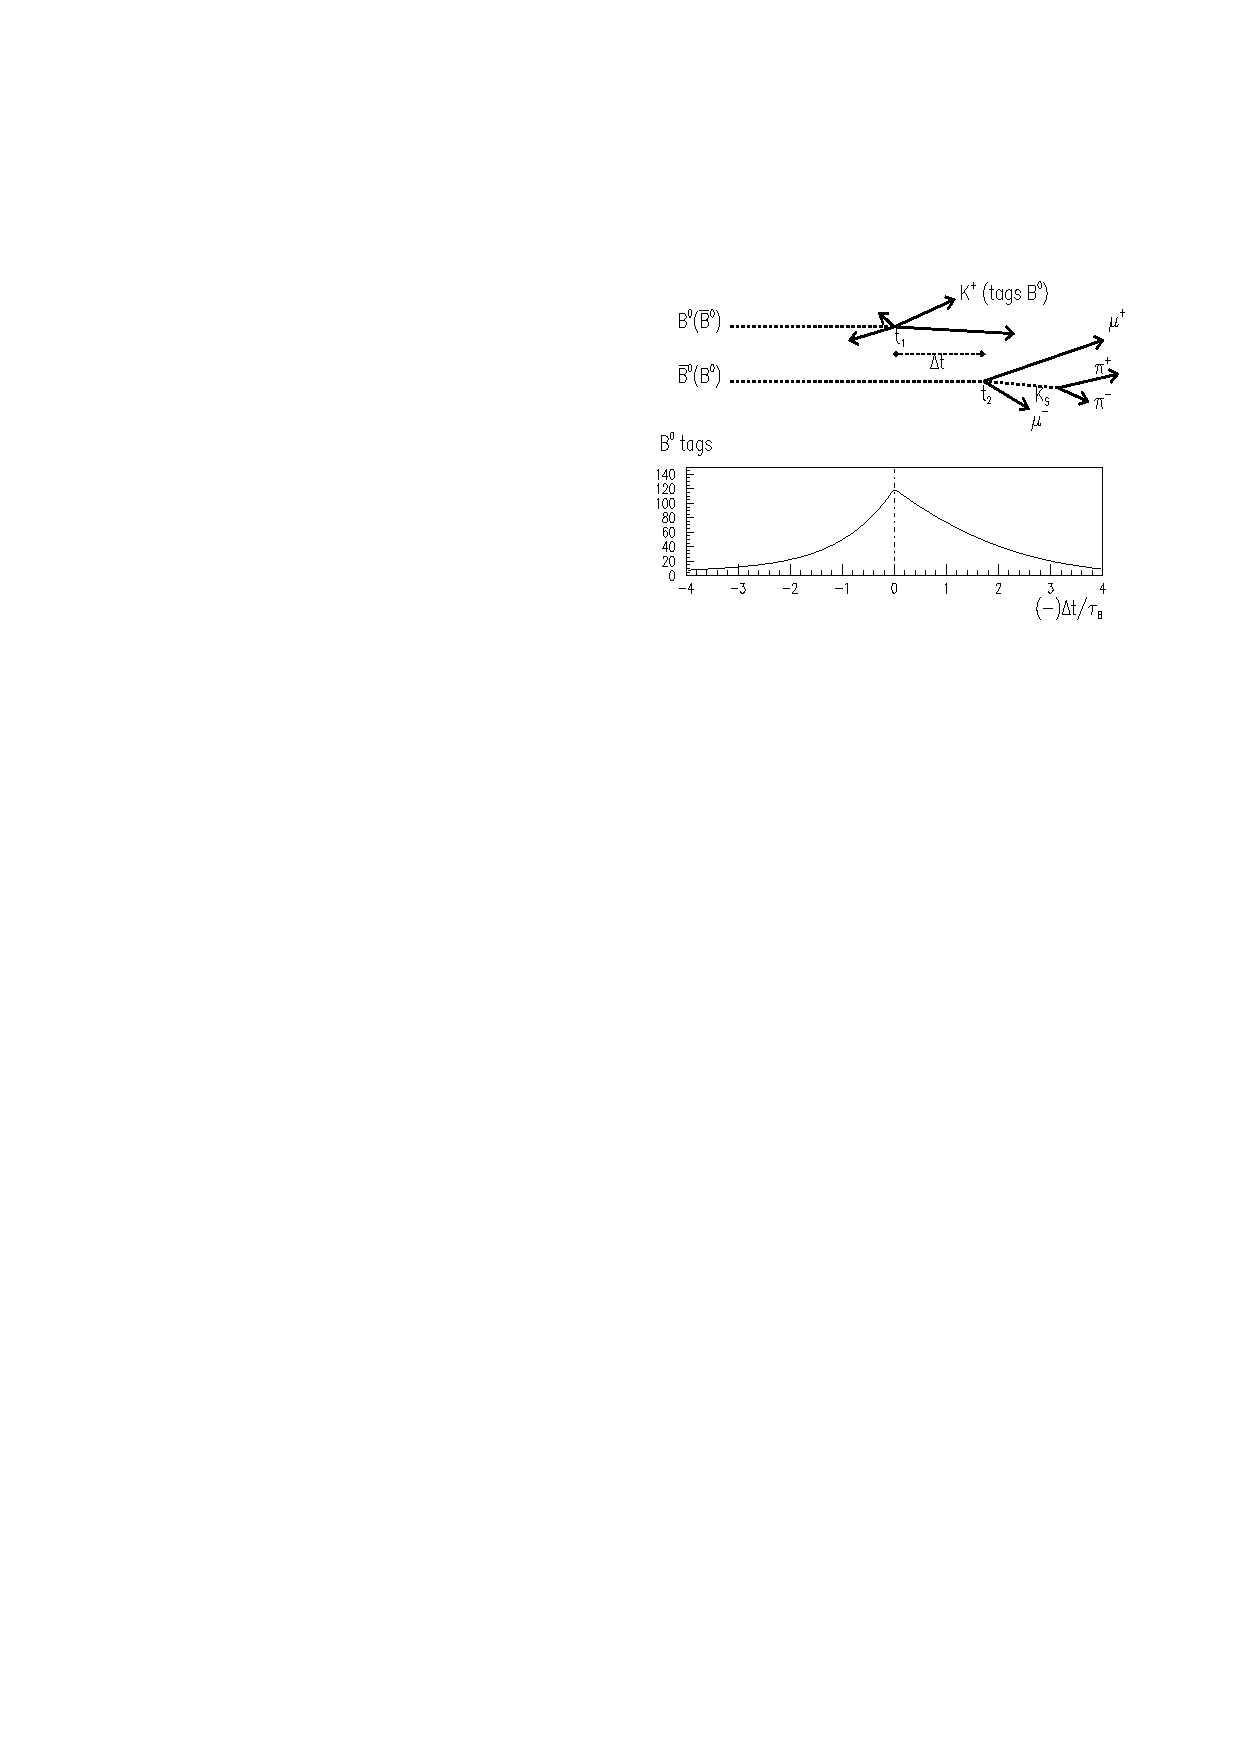
\includegraphics[width=\textwidth]{private/content/flavour-tagging/figs/b_factory_basic_principles}
\caption{Illustration of the measurement of \sintwobeta as conducted by the
\BFactories. \cite{Bevan:2014iga}}
\label{fig:flavour_tagging:lhcb:b_factory_basic_principles}
\end{figure}

\Cref{fig:flavour_tagging:lhcb:b_factory_basic_principles} illustrates the basic
principles of a \CP violation measurement at the \BFactories. The produced
$\Bd\Bdbar$ pair's wave function is in a $P$-wave entangled state, until one of
the mesons decays. From this point in space time ($t_1$) the second $\B$ meson
propagates further through the detector, mixes to its antimatter state, and
finally decays at $t_2$. The \CP asymmetry $\CPAsymmetry$ will therefore be a
function of the decay time difference $\Delta t$. This has two implications:
First, the decay time difference will always be computed relative to the
\enquote{tagging} \Bmeson decay and thus might be negative if the signal $\B$
meson decays first. Secondly, if the tagging \Bmeson decays into a
flavour-specific final state, this specifies the signal \Bmeson's flavour at
$\Delta t=0$.

As a result of the production mechanism, the fully reconstructed signal decay
leaves all remaining tracks to originate from the tagging $\B$. This allows to
classify the decay of the tagging meson according to the signature of the final
state particles. Specialised taggers then identify decays based on their
specific signature. In a second stage, all results provided by the single
taggers are combined into a final tagging decision. 

The lepton taggers deduce a tag from the charge of electrons and muons from
$\bquark \to \cquark \lepm \neutrinobar$ transitions in semileptonic $\B$
decays. Likewise, second order transitions from $\bquark \to \Wm \cquark ( \to
\squark \lepp \neutrino )$ can be used, but has to be handled differently as
their charge is opposite compared to primary leptons. Charged kaon candidates
from the $\bquark \to \cquark \to \squark$ decay chain reflect the charge of the
tagging meson. Here as well, kaons from second order transitions carry the
opposite charge. Charged pions from charm decays work as tagging particles
either directly or in events with both a pion and a charged kaon, the
correlation of the particles can be utilised to improve the tag decision.
Selecting high momentum particles, \eg fast pions from $\Bdbar \to \Dstarp
\pim$, is on its own another source of tagging information and might
additionally be correlated with slow particles to enhance the tagging result.
Finally the flavour of $\Lambda$ baryons from decays of the tagging $\B$ meson
can be exploited.

The \Babar experiment uses \acp{ANN} for each single tagger to provide several
intermediate tagging decisions that are subsequently combined using another \ANN
to gain a joined tagging decision. The effective tagging efficiency of the final
\Babar tagging algorithm is estimated on data to be $\efftageff = \SI{33.1 +-
0.3}{\percent}$. In \Belle analyses the flavour tagging approach is similar.
Instead of \acp{ANN} multi-dimensional look-up tables are used. At first,
information from charged tracks are looked-up to sort them into the signature
categories. Next, the received results are used on an event-level to provide the
final tagging decision. Using this approach an effective tagging efficiency of
$\efftageff = \SI{30.1 +- 0.4}{\percent}$ is achieved.

\subsection{\Acl{OS} algorithms}
\label{sec:flavour_tagging:os}
The \OS algorithms all infer the tagging decision from the quark flavour of the
\bhadron produced in association with the signal \Bmeson. If for example a $\Bu$
decays into a $\Kp X$ final state trough $\bquarkbar \to \cquarkbar \to
\squarkbar$ transition, it can unambiguously stated by looking at the kaon
charge that the \bhadron produced along with the $\Bu$ contained a $\bquarkbar$
quark. The tag identification for events with this signature fall into the scope
of the \OSK tagger.

In total four distinct \OS taggers, each developed for a special \OS decay
signature, provide tagging information. Besides the \OSK tagger, the \OSe and
the \OSm select leptons coming from the primary $\bquark \to X \lepm$ decay to
use their charge as an information carrier of the $\B$ flavour. Finally, the
\OSvtx tagger performs an inclusive reconstruction of the \OS \SV to then
compute a weighted sum of all particle track charges that originate from the
\SV. In the following the selection criteria and algorithms of the \OS taggers
are briefly described.

\missing{Intrinsic mistag due to neutral B meson oscillation}
 
\subsubsection{The \acl{OSK} tagger}
\label{sec:flavour_tagging:os:kaon}
The kaon tagger exploits the charge of kaons stemming from $\bquark \to
\cquark \to \squark$ decays of the opposite side \bhadron. As the charge of the
kaon is the opposite of the ancestor's charge, the kaon always carries the same
charge as the signal \Bmeson.

To reduce background contributions of prompt kaons and kaons from primary
$\bquarkbar \to \Wm (\to \cquark \squarkbar) \cquarkbar$ transitions, in which
case the kaon carries the \enquote{wrong} charge, several selection criteria are
applied. Cuts on the \pT, the \IP, the \IP/$\sigma_\text{\IP}$, and the track
fit \chisqndf are performed. \PID requirements on the \DLLKpi, the \DLLppi, and
\DLLmupi suppress mis-identified particles. Clone tracks are removed and kaon
candidates with originate from other \acp{PV} are rejected using a cut on the
\IP/$\sigma_\text{\IP}$ with respect to any \PV.
\cref{tab:flavour_tagging:os:kaon:cuts} lists all applied cuts. If more than one
tagging candidate is found, the decision obtained from the candidate with the
highest \pT is chosen. To further increase the effective tagging efficiency only
tag decisions are considered if the estimated mistag probability is smaller than
$\mathcal{P}=0.46$.

\begin{table}
  \centering
  \caption{Selection cuts for the \OSK tagger \cite{Grabalosa:2012qra}.}
  \label{tab:flavour_tagging:os:kaon:cuts}
  \begin{tabular}{ll}
    \toprule
    Property & Value \\
    \midrule
    \pT                                       & $>\SI{0.5}{\GeVc}$                  \\
    \IP                                       & $<\SI{1.25}{\milli\metre}$          \\
    \IP$/\sigma_\text{\IP}$                   & $>\num{3.35}$                       \\
    track fit \chisqndf                       & $<\num{2.75}$                       \\
    \DLLKpi                                   & $>\num{6}$                          \\
    $(\DLLKpi - \DLLppi)$                     & $>\num{-4}$                         \\
    \IP$/\sigma_\text{\IP}$ \wrt any \PV      & $>\num{4.5}$                        \\
    reject clone tracks & \\
    \bottomrule
  \end{tabular}
\end{table}

\subsubsection{The \acl{OSe} and the \acl{OSm} taggers}
\label{sec:flavour_tagging:os:lepton}

Leptons from $\bquark \to \cquark\Wboson$ transitions are selected in order to
deduce the opposite \bhadron charge. Thus positive lepton charge indicates a
$\bquark$ quark content of the signal \Bmeson and vice versa.

Cuts on the \PID and the lepton \pT are applied to reduce the mis-identification
rate and to suppress leptons from secondary decays of charm mesons. The muon
candidate purity is further enhanced by reducing fake muons, clone tracks, and
requiring a sufficient track fit quality. Electron candidate tracks must lie
inside the \HCAL acceptance and leave a substantial energy deposition in the
\ECAL compared to their momentum. To reduce backgrounds from photon conversions
close to the \proton\proton interaction region, a upper limit on the maximal
ionisation charge $Q_\text{\VELO}$ deposited in the \VELO is set. If more than
one lepton candidate passes the requirements, the one with the highest \pT is
chosen.

\begin{table}
  \centering
  \caption{Selection cuts for the \OSe and \OSm taggers
  \cite{Grabalosa:2012qra}, where $E$ is the particle energy measured in the
  \ac{ECAL} and $p$ the measured particle momentum. $Q_\text{\VELO}$ describes
  the ionisation charge deposit in the \VELO.}
  \label{tab:flavour_tagging:os:lepton:cuts}
  \begin{tabular}{ll}
    \toprule
    % general
    Property                                  & Value                               \\
    \midrule
    lepton \pT                                & $>\SI{1.2}{\GeVc}$                  \\
    muon \DLLmupi                             & $>\num{1}$                          \\
    muon track fit \chisqndf                  & $<\num{3.2}$                        \\
    \multicolumn{2}{l}{reject muon clone tracks and fake muons}                     \\
    electron \DLLepi                          & $>\num{4}$                          \\
    electron $E/p$                            & $>\num{0.8}$                        \\
    max. electron $Q_\text{\VELO}$            & $<\num{1.6}$                        \\
    \multicolumn{2}{l}{electron candidate track in \HCAL acceptance}                \\
    \bottomrule
  \end{tabular}
\end{table}

\subsubsection{The \acl{OSvtx} tagger}
\label{sec:flavour_tagging:os:vertex}

Besides the single particle taggers for kaons, muons, and electrons, the
\acl{OSvtx} tagger follows an alternative approach by trying to inclusively
reconstruct the decay vertex of the opposite \bhadron. Starting with a two-track
seed, matching tracks are appended and a weighted sum of the vertex charge is
calculated. The procedure is optimized using cuts on the considered tracks, the
seed properties, and the features of the reconstructed vertex.

The initial vertex seed is found by sampling track pairs from all particle
candidates surviving the following criteria: At least one of the tracks must be
a long track with a track fit quality of $\chisqndf<\num{2.5}$. To exclude poor
track reconstruction only tracks with an \IP uncertainty of
$\sigma_\text{\IP}<\num{1}$ are taken into account. Tracks from prompt particles
are rejected by a cut on the $2.5<\text{\IP}/\sigma_\text{\PV}<100$ \wrt the
\PV. Additionally the track has to have a $\pT>\SI{0.15}{\GeVc}$ and an
\IP$<\SI{3}{\milli\metre}$ \wrt to the \PV.\todo{Understand why the two IP
criteria are conflicting} The two seed tracks must be separated by an angle of
$\phi>\SI{1}{\mrad}$ and one of the tracks has to have a $\pT>\SI{0.3}{\GeVc}$.

For tracks pairs passing all selection criteria a vertex fit is performed. If
the fit succeeds and a fit quality of at least $\chisqndf<10$ is met, the fitted
vertex is considered as a seed. The seed is required to lie inside the detector
acceptance and in the forward direction of the \PV ($z>0$). \missing{Define
$r$-distance} The invariant mass of the seed is calculated and has to be greater
than $\SI{0.2}{\GeVcc}$ and not be compatible with the known $\KS$ or $\Lambdaz$
masses. % 0.490 < m_KS < 0.505 and 1.11 < m_Lambda < 1.12
A likelihood is computed for all seeds considering the vertex fit $\chisqndf$,
the minimum \pT, the maximum \PV \IP, the minimum \PV \IP$/\sigma_\text{\IP}$,
the angle between the seed tracks, the $r$-distance and the angle between the
seed direction \wrt to the \PV. Only seeds with a likelihood greater $\num{0.6}$
are further considered and the seed with the maximum likelihood is selected. The
seed algorithm successfully finds a seed in nearly $\SI{50}{\percent}$ of all
events and has a rate of $\SI{60}{\percent}$ to find a seed that is formed by
\bhadron decay products.

Subsequently more tracks are added to the seed. Additional tracks are required
to be compatible with the reconstructed seed vertex
(\IP$<\SI{0.9}{\milli\metre}$), have a \DOCA to any track in the seed smaller
than $\SI{0.2}{\milli\metre}$, the track fit quality is at least
$\chisqndf<\num{3}$, and are ruled out to be a clone track. Additionally the \IP
with respect to the \PV has to be larger than $\SI{0.1}{\milli\metre}$ and
$\text{\IP}/\sigma_\text{\IP}>\num{3.5}$.

After all tracks are added to the vertex another set of selection requirements
has to be fulfilled to optimize the effective tagging efficiency. The sum of all
track momenta has to be $\sum_i p_i > \SI{10}{\GeVc}$ and $\sum_i \pT(i) >
\SI{10}{\GeVc}$, the invariant vertex mass must be greater than $m_\text{vtx} >
\SI{0.5}{\GeVcc}$, the sum of the track
$\sum_i\text{\IP}_i/\sigma_{\text{\IP}_i}$ has to be larger $\num{10}$ and the
sum of the track \DOCA has to be $\sum_i\text{\acs{DOCA}}_i <
\SI{0.5}{\milli\metre}$.

The tag decision is then deduced from the inclusively reconstructed vertex by
calculating the weighted charge for all tracks $i$ forming the vertex
%
\begin{equation}\label{eq:flavour_tagging:os:vertex:charge}
  Q_\text{vtx} = \frac{\sum_i \pT^k(i)Q_i}{\sum_i\pT^k(i)}\eqcm
\end{equation}
where the track \acp{pT} are used as weights and the $k$ parameter is optimised
using simulated data to be $k=\num{0.4}$. In a final step, only charges of
$\vert Q_\text{vtx} \vert > 0.25$ are considered and the mistag probability has
to be smaller than $\mathcal{P}=0.46$.

\subsection{\Acl{SS} algorithms}
\label{sec:flavour_tagging:ss}

The \acl{SS} taggers exploit charge information from pions or kaons produced in
the hadronisation process of the signal \Bmeson. As illustrated in
\cref{fig:flavour_tagging:lhcb:schematics} the $\qqbar$ quark pair produced
alongside the signal meson, splits up to form the $\B$ meson and in the case of
a $\Bd$ ($\Bs$) an accompanying pion (kaon). Pions might also be produced in the
decay of excited $\B$ meson states.

\subsubsection{The \acl{SSpi} tagger}
\label{sec:flavour_tagging:ss:pion}

The pions from either the \Bmeson hadronisation or the decay of excited states
carry the same charge as the signal \Bmeson and are therefore suitable to
extract tagging information. The selection criteria pion candidates are required
to fulfil are listed in \cref{tab:flavour_tagging:ss:pion:cuts}. If more than
one pion candidate passes the requirements, the one with the highest \pT is
chosen. The tag decision has to have a mistag probability of $\mathcal{P}<0.46$,
otherwise the tag decision will be refused.
%
\begin{table}
  \centering
  \caption{Selection cuts for the \SSpi tagger \cite{Grabalosa:2012qra}, where
  $\Delta Q$ describes the mass difference of the $\Bd\pion$ mass and the $\Bd$
  mass.}
  \label{tab:flavour_tagging:ss:pion:cuts}
  \begin{tabular}{ll}
    \toprule
    Property                                  & Value                               \\
    \midrule
    \multicolumn{2}{l}{only long track pion candidates}                             \\
    \DLLKpi                                   & $<\num{4.5}$                        \\
    \DLLppi                                   & $<\num{15}$                         \\
    \pT                                       & $>\SI{0.5}{\GeVc}$                  \\
    $p$                                       & $>\SI{2.5}{\GeVc}$                  \\
    \PV $\text{\IP}/\sigma_\text{\IP}$        & $<\num{4}$                          \\
    $\Delta Q$                                & $<\SI{1.5}{\GeVcc}$                 \\
    \bottomrule
  \end{tabular}
\end{table}

\subsubsection{The \acl{SSK} tagger}
\label{sec:flavour_tagging:ss:kaon}

The charge of kaons produced together with a signal $\Bs$ meson can be exploited
in order to get a tag decision. The selection requirements for kaon candidates
are similar to those for the \SSpi tagger. Besides \PID variables, momenta, the
quality of the \IP fit and the track fit, differences between the $\Bs\kaon$
mass and the $\Bs$ mass, the difference in the $\phi$ angle between the signal
\Bmeson and the kaon, and the pseudo-rapidity between the signal \Bmeson and the
kaon are taken into account. If more than one candidate passes the criteria, the
one with the highest \pT is used. As this thesis presents a measurement in the
decay of $\Bd$ and $\Bdbar$ mesons, where the kaon tagger is not used, no
further details will be given and an emphasis is placed on the \SSpi tagger.
% %
% \begin{table}
%   \centering
%   \caption{Selection cuts for the \SSK tagger \cite{Grabalosa:2012qra}, where
%   $\Delta Q$ describes the mass difference of the $\Bs\kaon$ mass and the $\Bs$
%   mass, $\vert \Delta\phi \vert$ the difference in the $\phi$ angle between the
%   signal \Bmeson and the kaon, $\vert \Delta\eta \vert$ the pseudo-rapidity
%   between the signal \Bmeson and the kaon, and $\vert \Delta R \vert =
%   \sqrt{\Delta\eta^2 + \Delta\phi^2}$.}
%   \label{tab:flavour_tagging:ss:kaon:cuts}
%   \begin{tabular}{ll}
%     \toprule
%     Property                                  & Value                               \\
%     \midrule
%     \DLLKpi                                   & $>\num{4.5}$                        \\
%     (\DLLKpi - \DLLppi)                       & $>\num{-8.5}$                       \\
%     \pT                                       & $>\SI{0.75}{\GeVc}$                 \\
%     $p$                                       & $>\SI{5.25}{\GeVc}$                 \\
%     \PV $\text{\IP}/\sigma_\text{\IP}$        & $<\num{4.125}$                      \\
%     track $\chisqndf$                         & $<\num{3.75}$                       \\
%     $\Delta Q$                                & $<\SI{1.5}{\GeVcc}$                 \\
%     $\vert \Delta\phi \vert$                  & $<\num{0.7}$                        \\
%     $\vert \Delta\eta \vert$                  & $<\num{0.525}$                      \\
%     $\vert \Delta R \vert$                    & $<\num{1.2}$                        \\
%     \bottomrule
%   \end{tabular}
% \end{table}

\section{Calibration of the flavour tagging output}
\label{sec:flavour_tagging:calibration}

The tagging decisions each tagger estimates are based on selection criteria
developed using simulations and flavour-specific decays. While the tag decision
$d$ depends on a measured particle or vertex charge, the mistag estimate
$\mistagestimate$ is computed using \acp{ANN} trained on \sweighted $\BuToJpsiK$
data incorporating kinematic and geometric event properties.

In order to adjust for differences between the training and physics data, the
\ANN output is calibrated using flavour-specific decays. For the \OS taggers and
the \SSpi tagger, $\BuToJpsiK$ decays are used to develop a calibration function
$\omofeta$ (while the data sample that was used to train the \ANN before is
omitted). Decays of charged \Bmesons are not subject to quark mixing, thus, the
true mistag probability $\omega$ can be determined directly by counting and
comparing the final state charges. In case of neutral $\B$ decays into
flavour-specific final states a full time-dependent mixing analysis is
necessary.

In \cref{sec:flavour_tagging:calibration:method} general concepts and the choice
of the calibration function are presented, then the methodologies of a
calibration using decays of either charged or neutral \Bmesons is explained. Two
different approaches how to incorporate the per-event tagging information are
described and an outlook into the technique of combining different tagger's
output into a single tag decision is given. Then the calibration of the \OS and
the \SSpi taggers using $\BuToJpsiK$ and $\BdToJpsiKstar$ decays is shown in
\cref{sec:flavour_tagging:calibration:os,sec:flavour_tagging:calibration:ss}.

\subsection{Methodology}
\label{sec:flavour_tagging:calibration:method}

The calibration of the flavour tagging output usually follows an iterative
procedure. All single taggers and the combination of all \OS tagging decisions
(see \cref{sec:flavour_tagging:combination}) is calibrated using the high yield
decay channel $\BuToJpsiK$. The correction determined in this step is then
applied to the tagging algorithms during the common data processing stage
(\enquote{Stripping}). Afterwards, the calibration is checked on several control
channels, \ie $\BuToJpsiK$, $\BuToDpi$, $\BdToJpsiKstar$, $\BdToDpi$,
$\BdToDstarmunu$ and $\BsToDspi$ and possible small corrections can be applied
for individual analyses. Assuming no correlations amongst the single taggers, it
can be assumed, that the calibration is still valid for the combined tagging
estimates. This assumption is checked as well.

The calibration function $\omofeta$ is chosen linear with two parameters
$\pzero$ and $\pone$,
%
\begin{equation}\label{eq:flavour_tagging:calibration:method:calibration}
  \omofeta = \pzero + \pone (\mistagestimate - \avgmistagestimate)\eqcm
\end{equation}
%
with $\avgmistagestimate$ being the average mistag estimate used to decorrelate
$\pzero$ and $\pone$. Hence, a perfect calibrated tagging output would result in
$\pzero = \avgmistagestimate$ and $\pone = 1$. The performance of the tagging
algorithms may depend on the flavour of the initial \Bmeson. Different
interaction of particles, \eg kaons used by the \OSK tagger, induce deviating
reconstruction efficiencies, resulting in different tagging efficiencies
$\tageff$ and mistag probabilities $\mistag$ for initial $\Bd$ and $\Bdbar$
states. To correct for asymmetries of the tagging calibration, two independent
calibration functions are defined
%
\begin{equation}\label{eq:flavour_tagging:calibration:method:asymmetric_calibration:omega}
  \begin{split}
    \omofetaBd    &= \pzeroBd    + \poneBd    (\mistagestimate - \avgmistagestimate)\eqcm \\
    \omofetaBdbar &= \pzeroBdbar + \poneBdbar (\mistagestimate - \avgmistagestimate)\eqcm
  \end{split}
\end{equation}
%
where the calibration parameters $\p{i}{}$ (with $i=0,1$) can be parametrised as
%
\begin{equation}\label{eq:flavour_tagging:calibration:method:asymmetric_calibration:ps}
  \p{i}{\Bd} = \p{i}{} + \frac{\deltap{i}{}}{2} \eqspace\text{and}\eqspace \p{i}{\Bdbar} = \p{i}{} - \frac{\deltap{i}{}}{2}\eqpd
\end{equation}

\subsubsection{Flavour tagging calibration using decays of charged \Bmesons}
\label{sec:flavour_tagging:calibration:method:charged}

Using decays of charged \Bmesons into flavour-specific final states like
$\BuToJpsiK$ and $\BuToDpi$ is the straightforward way to calibrate the flavour
tagging. The decisions given by the tagging algorithms can be easily compared to
the final state charges without ambiguities due to oscillations in the \Bmeson
system.

Using a fit to the $\Bu$ mass distribution the background contributions can be
subtracted using the \sPlot technique. The mistag estimate distribution can then
be split into $n$ bins to compare the average estimated mistag of each bin
$\mistagestimate_i$ to the counted mistag ratio $\mistag_i$.
\Cref{fig:flavour_tagging:calibration:method:charged:calibration_plot} shows an
exemplary calibration plot using a dataset of $\BuToJpsiK$ decays corresponding
to an integrated luminosity of $\SI{0.37}{\per\femtobarn}$ \cite{Aaij:2012mu}.
The data is categorised into $\num{21}$ bins of $\mistagestimate$ and a linear
function is fit to the data to estimate the calibration parameters $\pzero$ and
$\pone$.
%
\begin{figure}
\centering
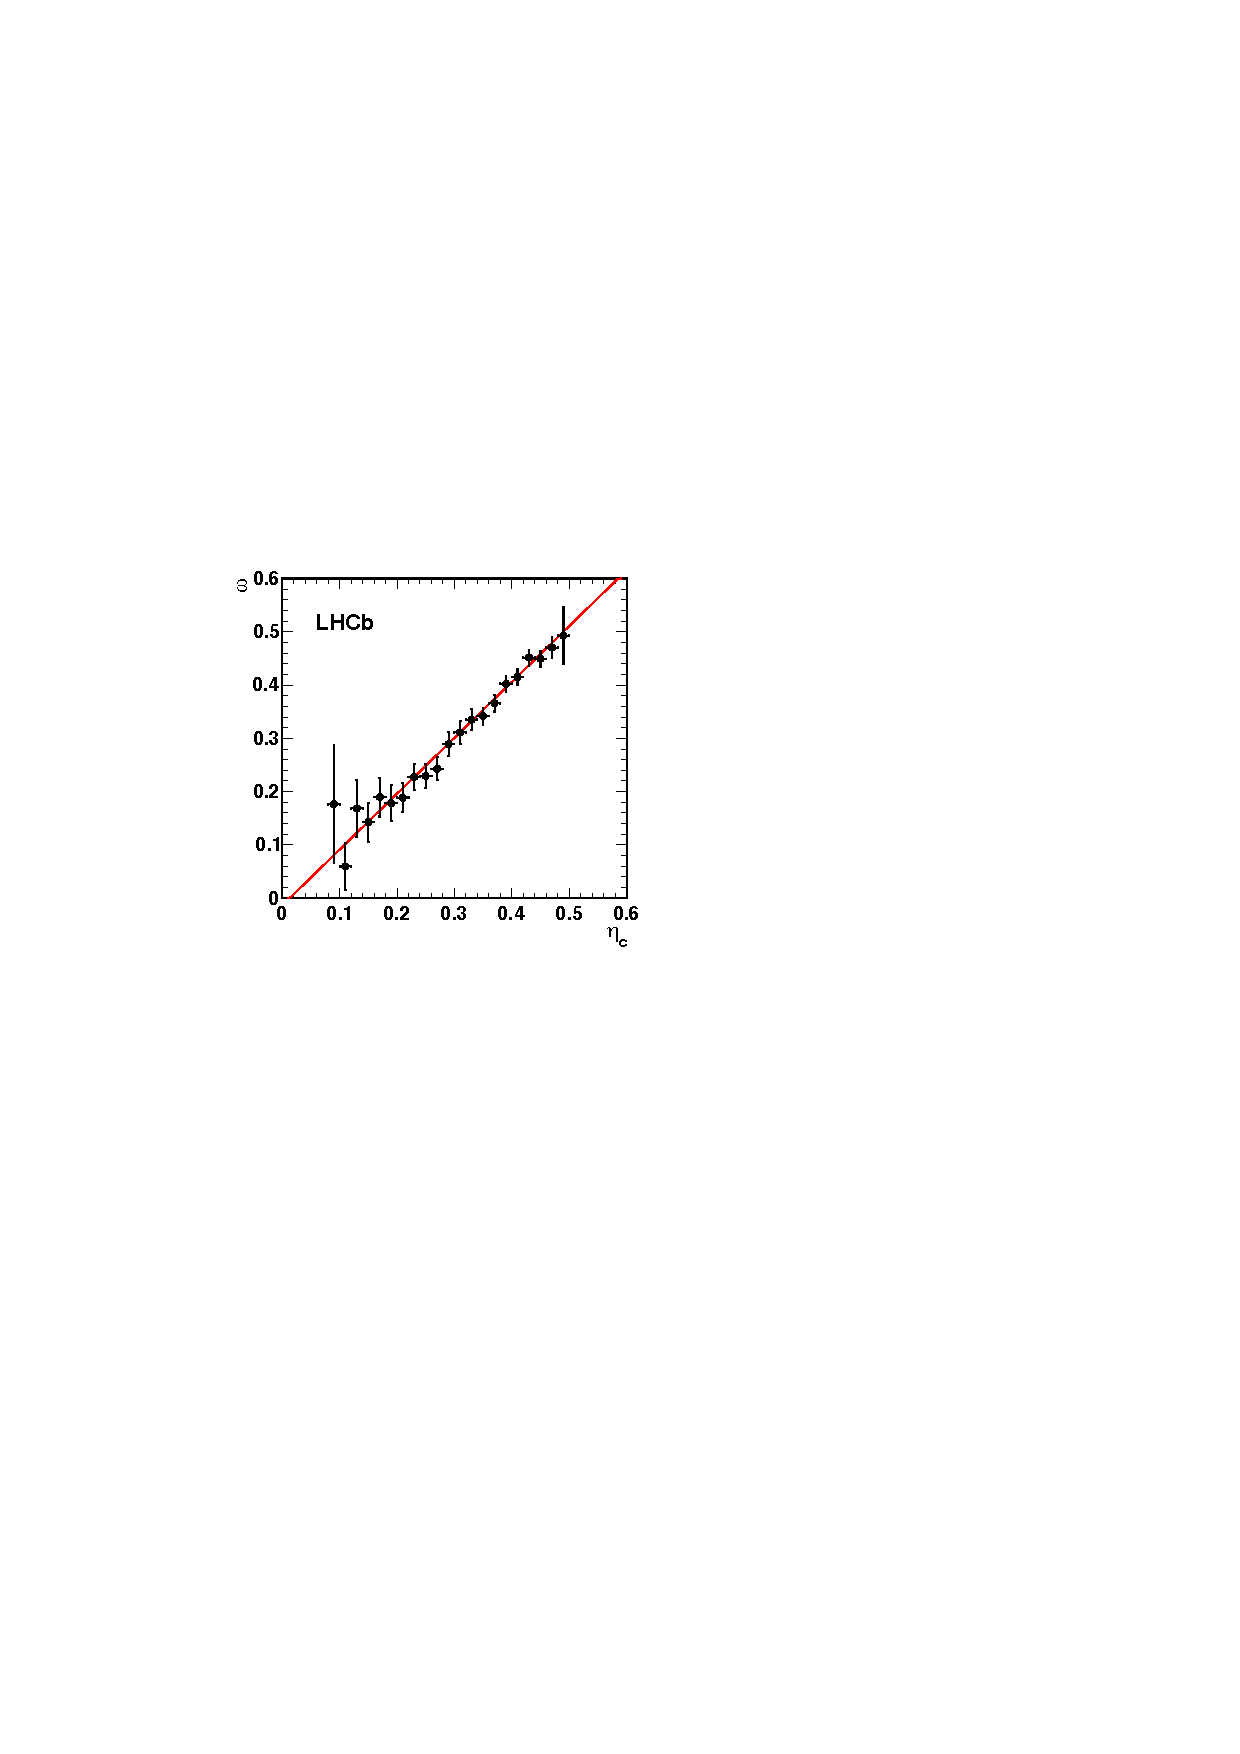
\includegraphics[width=0.5\textwidth]{private/content/flavour-tagging/figs/lhcb_ft_calibration_bu2jpsik_037fb}
\caption{Measured mistag fraction $\mistag$ plotted against the mistag estimate
$\mistagestimate$ provided by the tagging algorithms. Described in black are
data of $\BuToJpsiK$ decays corresponding to an integrated luminosity of
$\SI{0.37}{\per\femtobarn}$. The red line illustrates the linear calibration
function fitted to the data. \cite{Aaij:2012mu}}
\label{fig:flavour_tagging:calibration:method:charged:calibration_plot}
\end{figure}

As an alternative, the calibration function can be implemented into the unbinned
maximum likelihood fit to the dimensions: mass, tagging decision, and mistag
probability estimate. Using a conditional \PDF
$\Prob{}{\Sig}(\tagdecision,\tagdecision^\prime,\mistagestimate)$, where
$\tagdecision^\prime$ describes the true $\Bu$ tag derived from the final-state
particle charge.
%
\begin{equation}
  \Prob{}{\Sig}(\tagdecision,\tagdecision^\prime,\mistagestimate) = 
  \begin{cases}
        \tageff (1-\omofeta) \Prob{}{\Sig}(\mistagestimate)    & \text{if $\tagdecision =    \tagdecision^\prime$} \\
        \tageff    \omofeta  \Prob{}{\Sig}(\mistagestimate)    & \text{if $\tagdecision \neq \tagdecision^\prime$} \\
    1 - \tageff                                                & \text{if $\tagdecision = 0$} \\
  \end{cases}
\end{equation}
%
\info{Try to understand better, how the calibration using per-event information works on charged channels.}

\subsubsection{Flavour tagging calibration using decays of neutral \Bmesons}
\label{sec:flavour_tagging:calibration:method:neutral}

In the decay of neutral \Bmesons the oscillation of the propagating $\B$ state
prevents the determination of the initial flavour just by measuring the final
state charge. Instead a full decay time dependent mixing analysis has to be
performed. As described in \cref{sec:missing}\addref{Mixing asymmetry} the signal mixing asymmetry is
given by
%
\begin{equation}
  \MixingAsymmetry = (1 - 2\mistag)\cos(\dmd t)\eqpd
\end{equation}
%
This can be either utilised in a simultaneous fit in different bins of
$\mistagestimate$ to extract per bin $\mistag_i$, then following the same
procedure as described for charged initial states or by implementing the
calibration function $\omofeta$ directly into the \PDF.

\subsection{\ac{OS} tagger calibration using BuToJpsiK decays}
\label{sec:flavour_tagging:calibration:os}

Deviating from the standard procedure to calibrate the \OS taggers and their
combination using a set of physics channels, only $\BuToJpsiK$ is used. A
previous study \cite{Aaij:1497268} made apparent that the uncertainties arising
from the flavour tagging calibration provide the largest contribution to the
overall systematic uncertainties on the measured quantities $\SJpsiKS$ and
$\CJpsiKS$. Therefore, going without semileptonic and fully hadronic decay modes
with different kinematic properties and only use $\BuToJpsiK$ decays with a
nearly similar final state, can reduce the uncertainties. An additional
cross-check of the calibration is performed on $\BdToJpsiKstar$ decays to
confirm the portability of the calibration on a $\Bu$ to a $\Bd$ initial state.
\missing{\OS calibration: $\BuToJpsiK$ signal selection?}

The calibration then follows the already outlined approach: extracting \sweights
by a fit to the \Bu mass distribution, then comparing the true fraction of wrong
tagged candidates to the average mistag estimate in $\num{60}$ $\mistagestimate$
bins. The mass model used in the fit is a sum of three Gaussian \acp{PDF} with a
shared mean to describe the signal shape and an exponential \PDF for the
background contributions. The fit to the $(\mistagestimate_i,\mistag_i)$ pairs
using \cref{eq:flavour_tagging:calibration:method:calibration} yields
%
\begin{equation}\label{eq:flavour_tagging:calibration:os:parameters}
  \begin{split}
    \p{0}{\text{OS}} &= 0.3815 \pm 0.0011 \text{\,(\stat)} 
                               \pm 0.0015 \text{\,(\syst type I)}  
                               \pm 0.0005 \text{\,(\syst type II)} \eqcm\\ % total syst 0.0016 
    \p{1}{\text{OS}} &= 0.978\phantom{0} \pm 0.012\phantom{0} \text{\,(\stat)} 
                                         \pm 0.006\phantom{0}  \text{\,(\syst type I)} 
                                         \pm 0.007\phantom{0}  \text{\,(\syst type II)} \eqcm\\ % total syst 0.009
    \langle\mistagestimate^{\text{OS}}\rangle &= 0.3786 \eqcm \\
    \rho_{p_0,p_1} &= 0.14 \eqcm
  \end{split}
\end{equation}
%
where $\rho_{p_0,p_1}$ is the correlation between $\p{0}{\text{OS}}$ and
$\p{0}{\text{OS}}$. \Cref{fig:flavour_tagging:calibration:os:mass_and_calibration}\addref{BuToJpsiK calibration, how?} 
shows the mass distribution and the \PDF projection as well as the calibration
plot.
%
\begin{figure}
\centering
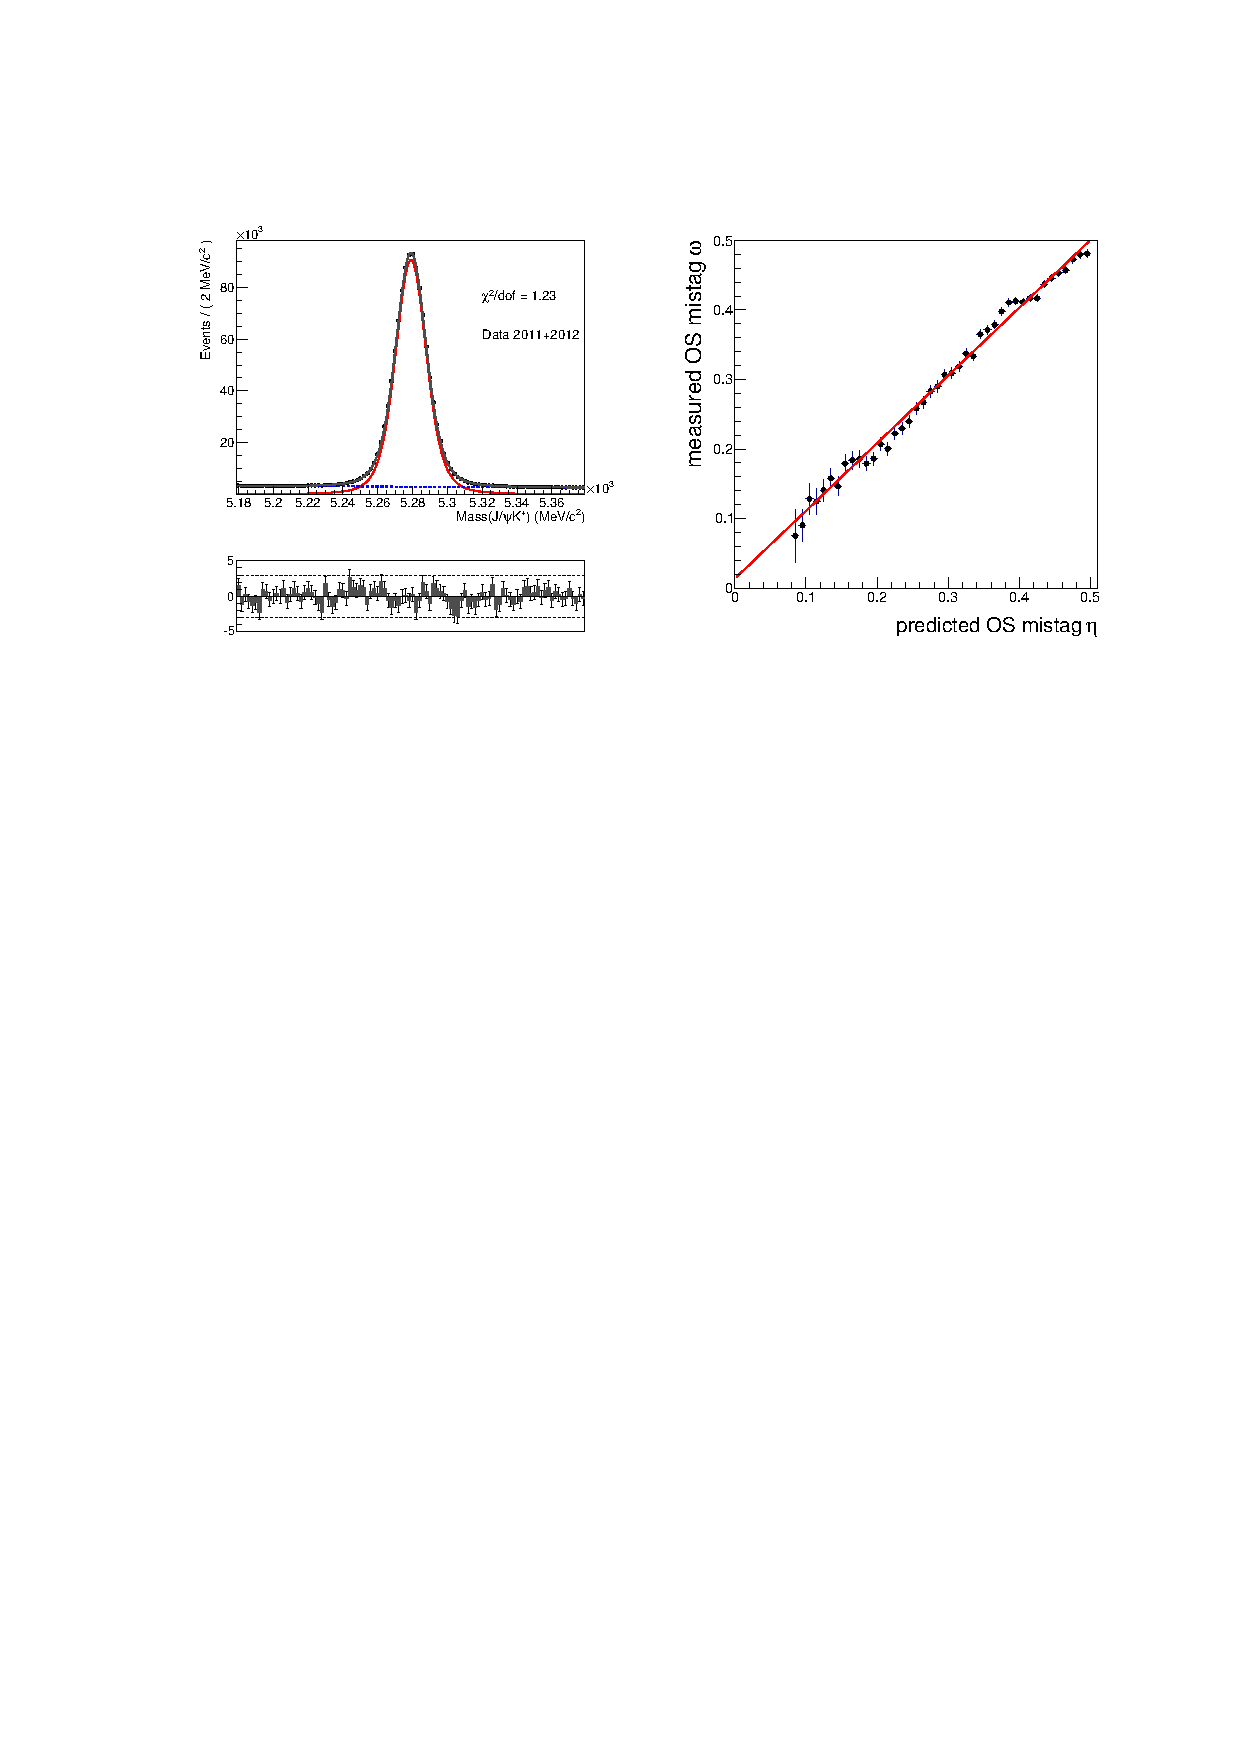
\includegraphics[width=\textwidth]{private/content/flavour-tagging/figs/lhcb_ft_calibration_bu2jpsik_3fb}
\caption{(a) Distribution of $\BuToJpsiK$ mass and projection of the fit \PDF.
The black solid line shows the total mass \PDF, the red solid line the signal
and the blue dashed line the background component. (b) Distribution of
$(\mistagestimate_i,\mistag_i)$ pairs in the decay $\BuToJpsiK$ together with
the linear calibration function in red. \cite{FT:RunI}}
\label{fig:flavour_tagging:calibration:os:mass_and_calibration}
\end{figure}
%
The asymmetries in the mistag probabilities are determined by repeating the
measurement when splitting the data sample into the initial $\Bd$ flavours and
comparing the values for $\pzero$ and $\pone$. The results are
%
\begin{equation}\label{eq:flavour_tagging:calibration:os:asymmetries}
  \begin{split}
    \deltap{0}{\text{OS}} &= p_0^{\text{OS,\Bd}}-p_0^{\text{OS,\Bdbar}} \\
                          &= 0.0148 \pm 0.0016 \text{\,(\stat)} \pm  0.0007 \text{\,(\syst type I)} \pm  0.0004 \text{\,(\syst type II)} \eqcm \\ % total syst. 0.0008
    \deltap{1}{\text{OS}} &= p_1^{\text{OS,\Bd}}-p_1^{\text{OS,\Bdbar}} \\
                          &= 0.070\phantom{0} \pm 0.018\phantom{0} \text{\,(\stat)} \pm 0.003\phantom{0} \text{\,(\syst type I)} \pm 0.002\phantom{0} \text{\,(\syst type II)} \eqcm \\ % total syst. 0.004
    \Delta \tageff^{\text{OS}} &= \tageff^{\text{OS,\Bd}} - \tageff^{\text{OS,\Bdbar}} = (-0.09  \pm 0.09 \text{\,(\stat)} \pm   0.09 \text{\,(\syst)})\% \eqpd
  \end{split}
\end{equation}
%
As the difference in the tagging efficiencies $\Delta \tageff^{\text{OS}}$ is
compatible with zero, it is neglected in the following.
\missing{Description of determination of systematics}
\missing{Comparison of $\BuToJpsiK$ and $\BdToJpsiKstar$}

\subsection{\ac{SS} tagger calibration using BdToJpsiKstar decays}
\label{sec:flavour_tagging:calibration:ss}

\info{How to handle the \SSpi precalibration for \Davinci versions prior to v35r1}
%
The \SSpi tagger is calibrated using a dataset of $\BdToJpsiKstar$ decays
corresponding to an integrated luminosity of $\SI{3.0}{\per\fb}$ collected by
the \LHCb experiment in \RunOne. As the \SSpi tagging algorithm depends on the
fragmentation process of the initial \Bmeson, a $\Bd$ decay mode is preferred
over a decay of $\Bu$ mesons.
\missing{\OS calibration: $\BdToJpsiKstar$ signal selection?}

To describe the mixing asymmetry $\MixingAsymmetry$ a two-dimensional fit to the
reconstructed decay time and mass distribution is performed. The signal mass
component is described by an Ipatia \PDF \cite{} with all tail parameters fixed
to values determined on simulations. The description of the combinatorial
background component consists of an exponential \PDF. The decay time signal \PDF
contains an acceptance function $\eps(t)$ describing reconstruction and
selection inefficiencies and a convolution of a $\B$ mixing \PDF and a
resolution model
%
\begin{equation}
  \Prob{\Sig}{} = \eps(t) \cdot \left[ \Prob{\text{mix}}{}(t, \tagdecision, \tagdecision^\prime, \mistagestimate) \otimes \mathcal{R}(t - t_\text{true}) \right] \eqcm
\end{equation}
%
with
%
\begin{equation}
  \Prob{\text{mix}}{}(t, \tagdecision, \tagdecision^\prime, \mistagestimate) 
  \propto 
  \exponential{-\sfrac{t}{\tau}} \left( 1 - \tagdecision \Delta\omofeta + \tagdecision \tagdecision^\prime (1 - 2 \langle\omofeta\rangle) \cos(\dmd t) \right)\eqcm
\end{equation}
%
where the acceptance function is parametrised as
%
\begin{equation}
  \eps(t) = \arctan(t \exponential{\alpha t+ \beta})\eqpd
\end{equation}

\newpage
\section{Combination}
\label{sec:flavour_tagging:combination}
Combination of OS and SS tagging, FT correlations

\section{Performance}
\label{sec:flavour_tagging:performance}
Performance of the FT algorithms

\section{Recent developments}
\label{sec:flavour_tagging:developments}

\section{Influence on the measurement of sin2beta}
\label{sec:flavour_tagging:sin2beta}
effect on dilution of asymmetry
influence on measuring sin2beta, Dilution

\FloatBarrier

% %%%%%%%%%%%%%%%%%%%%%%%%%%%%%%%%%%%%%%%%%%%%%%%%%%%%%%%%%%%%%%%%%%%%%%%%%%%%%%
%!TEX root = ../../common/main.tex

\section{Backgrounds}
\label{sec:measurement_of_sin2beta:physic_backgrounds}

This section describes the evaluation of background contributions in the data.
Besides combinatorial background from particles combined by chance with
properties that allow to pass all selection steps two other sources are
investigated: physics backgrounds from decays with mis-identified final state
particles are studied in
\cref{sec:measurement_of_sin2beta:physic_backgrounds:physic_backgrounds} and the
influence of non-uniform tagging responses for the background candidates is
examined in
\cref{sec:measurement_of_sin2beta:physic_backgrounds:tagging_asymmetries}.

% ------------------------------------------------------------------------------
\subsection{Physics backgrounds}
\label{sec:measurement_of_sin2beta:physic_backgrounds:physic_backgrounds}

To ensure that the background consists of combinatorial backgrounds, and that
exclusive backgrounds are negligible, possible physics backgrounds are studied
with simulated data (see \cref{sec:measurement_of_sin2beta:data_preparation:datasamples:mc}). 

Using the true particle identities from \MC reveals the existence of remnants
from physic backgrounds in the $\inclJPsi$ and the $\BdToJpsiX$ \MC samples. In
the $\BdToJpsiX$, around $\SI{0.04}{\percent}$ $\BdToJpsiKstar$ candidates
survive the applied selection criteria compared to $\SI{0.5}{\percent}$ signal
events. In the $\inclJPsi$ sample $\SI{0.0005}{\percent}$ $\BdToJpsiKstar$,
$\SI{0.0002}{\percent}$ $\BsToJpsiKS$, and $\SI{0.0002}{\percent}$
$\LbToJpsiLambda$ background events contribute, compared to
$\SI{0.01}{\percent}$ $\BdToJpsiKS$ candidates.

Since the production of $\Bs$ is a factor $\num{100}$ less frequent than the
$\Bd$ and reconstructed $\BsToJpsiKS$ candidates lie outside the nominal mass
range, we neglect possible contributions. While $\BdToJpsiKstar$ background
results from kaon-pion mis-identification, $\LbToJpsiLambda$ candidates are
found in the sample due to a proton-pion mis-identification. Their expected
contribution in the data sample is further studied by using signal \MC samples
of $\BdToJpsiKstar$ and $\LbToJpsiLambda$.

\subsubsection{Physics backgrounds from $\kaon$-$\pion$ mis-ID}
\label{sec:measurement_of_sin2beta:physic_backgrounds:physic_backgrounds:kstar}

In the $\BdToJpsiKstar$ signal \MC $\SI{0.3}{\percent}$ of $\num{4e6}$ generated
background candidates get reconstructed and survive the applied stripping cuts.
This number already reduces to $\SI{0.004}{\percent}$ after applying cuts on the
nominal mass and time ranges. After the full offline selection, considering a
$\SI{38}{\percent}$ tagging efficiency, and scaling the numbers to match a data
sample corresponding to $\SI[separate-uncertainty=true]{3}{\per\femto\barn}$
integrated luminosity, $\num{20}$ $\BdToJpsiKstar$ candidates with a positive
\MC information match remain. This corresponds to a fraction of roughly
$\SI{0.04}{\percent}$ of the background in the nominal data sample. The source
of the remaining contributions are \eg decays like
$\decay{\Bdstar}{\Bd(\to\jpsi\Kstarz)\,\Xparticle}$.

\subsubsection{Physics backgrounds from $\proton$-$\pion$ mis-ID}
\label{sec:measurement_of_sin2beta:physic_backgrounds:physic_backgrounds:lambda}

Out of $\num{3e6}$ generated $\LbToJpsiLambda$ signal candidates only
$\SI{2.0}{\percent}$ get reconstructed and pass the stripping. The cuts on the
nominal mass and time ranges reduce this number down to $\SI{0.32}{\percent}$.
The veto cut applied in the offline selection (see
\cref{sec:measurement_of_sin2beta:data_preparation:offline_selection:daughters})
decreases the number of candidates inside this mass and decay time window by
more than $\SI{50}{\percent}$ to $\SI{0.15}{\percent}$. After applying the full
offline selection, including the tagging efficiency, and scaling the sample to
correspond to the collected integrated luminosity in data, $\num{120}$ MC
truth-matched $\LbToJpsiLambda$ candidates remain. Therefore, we expect a
$\SI{0.2}{\percent}$ contribution of $\LbToJpsiLambda$ background candidates in
our nominal data sample.

% ------------------------------------------------------------------------------
\subsection{Background tagging asymmetries}
\label{sec:measurement_of_sin2beta:physic_backgrounds:tagging_asymmetries}
\missing{Background tagging asymmetries}

\FloatBarrier

% %%%%%%%%%%%%%%%%%%%%%%%%%%%%%%%%%%%%%%%%%%%%%%%%%%%%%%%%%%%%%%%%%%%%%%%%%%%%%%
%!TEX root = ../../common/main.tex

\section{Decay time resolution and acceptance}
\label{sec:measurement_of_sin2beta:resolution_and_acceptance}

In the following sections the influence of the decay time resolution and
acceptance effects are studied. 

% ------------------------------------------------------------------------------
\subsection{Resolution}
\label{sec:measurement_of_sin2beta:resolution_and_acceptance:resolution}

In this section the applicability of the \dtfpv output variable $\obsTimeError$ as
the per-event decay time error resolution estimate is checked and a model to
calibrate the estimate is developed. The model is determined in a two step
procedure. At first different calibration models are tested using a binned fit
on the decay time resolution determined on data as a function of the resolution
estimate $\obsTimeError$. Then the resolution model is used in an unbinned
likelihood fit to determine the calibration parameter values.

The study is performed on $\BdToJpsiKS$ candidates passing the pre-scaled
stripping line. The nominal selection is applied, except the decay time cut at
$\obsTime < \SI{0.3}{\pico\second}$, all remaining candidates are considered
irrespective of their tagging information. Without cuts restricting the
reconstructed decay time of the \Bd candidates, the sample consist mainly of
combinatorial background candidates promptly produced at the \PV. Studies on
simulated data have shown\addref{Reso study on MC}, that the decay time
resolution of prompt candidates is compatible to the resolution of signal
candidates. Thus, the resolution found for the prompt candidates can be used. A
fit to the $\Jpsi$ candidate's reconstructed mass is applied to get signal
\sweights that are subsequently used in a weighted likelihood fit to the
reconstructed \Bd candidates decay time distribution.

The $\Jpsi$ mass distribution is described by an Ipatia \PDF (\cf
\cref{sec:measurement_of_sin2beta:likelihood_fit:pdfs:ipatia}) for the signal
component and an exponential \PDF for the background candidates. The fit is
performed on the reconstructed invariant dimuon mass $m_{\mumu}$ in a range from
$\SI{3040}{\MeVcc}$ to $\SI{3155}{\MeVcc}$. The fitted distribution and the \PDF
projections split into the \catDD and \catLL categories are shown in 
\cref{fig:measurement_of_sin2beta:resolution_and_acceptance:resolution:jpsi_mass}.
%
\begin{figure}[h]
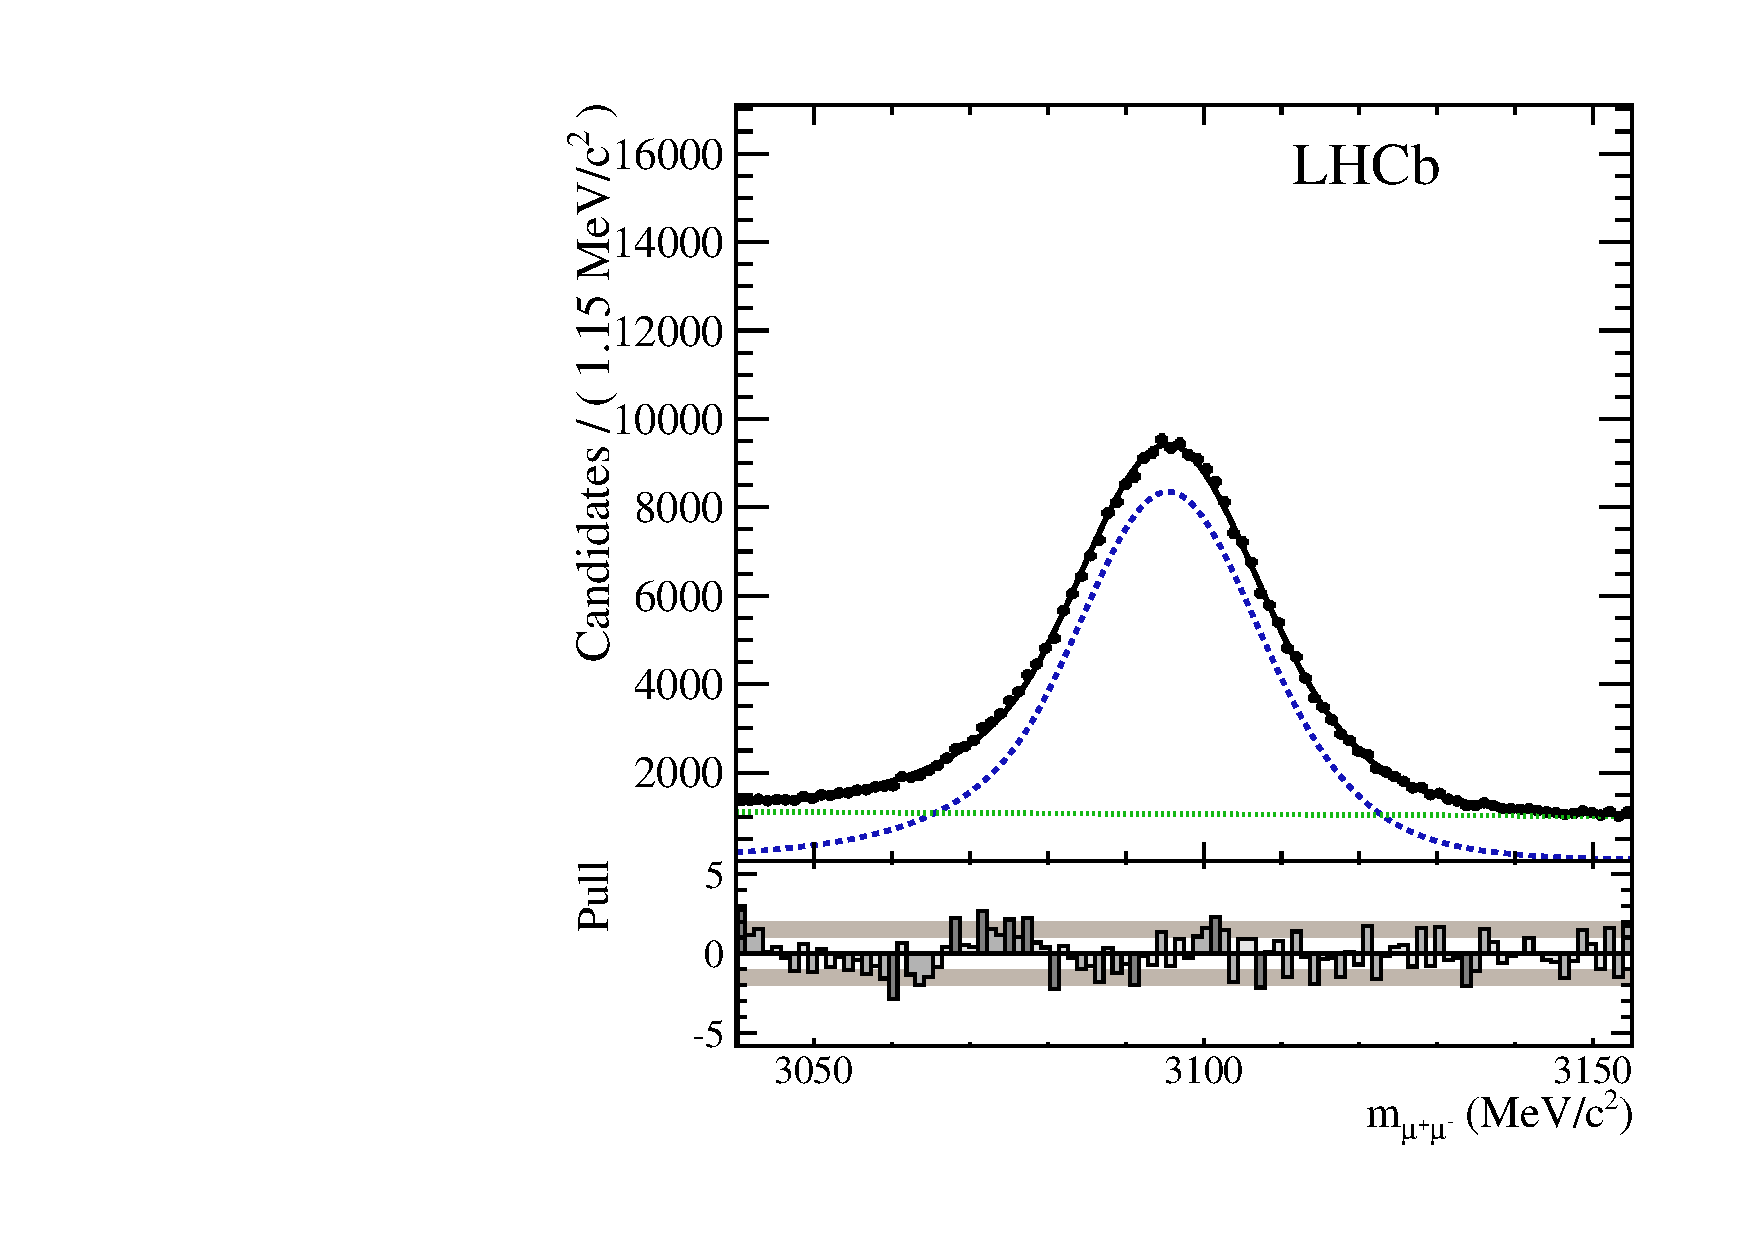
\includegraphics[width=0.49\textwidth]{private/content/measurement-of-sin2beta/figs/resolution_mass_jpsi_dd.pdf}
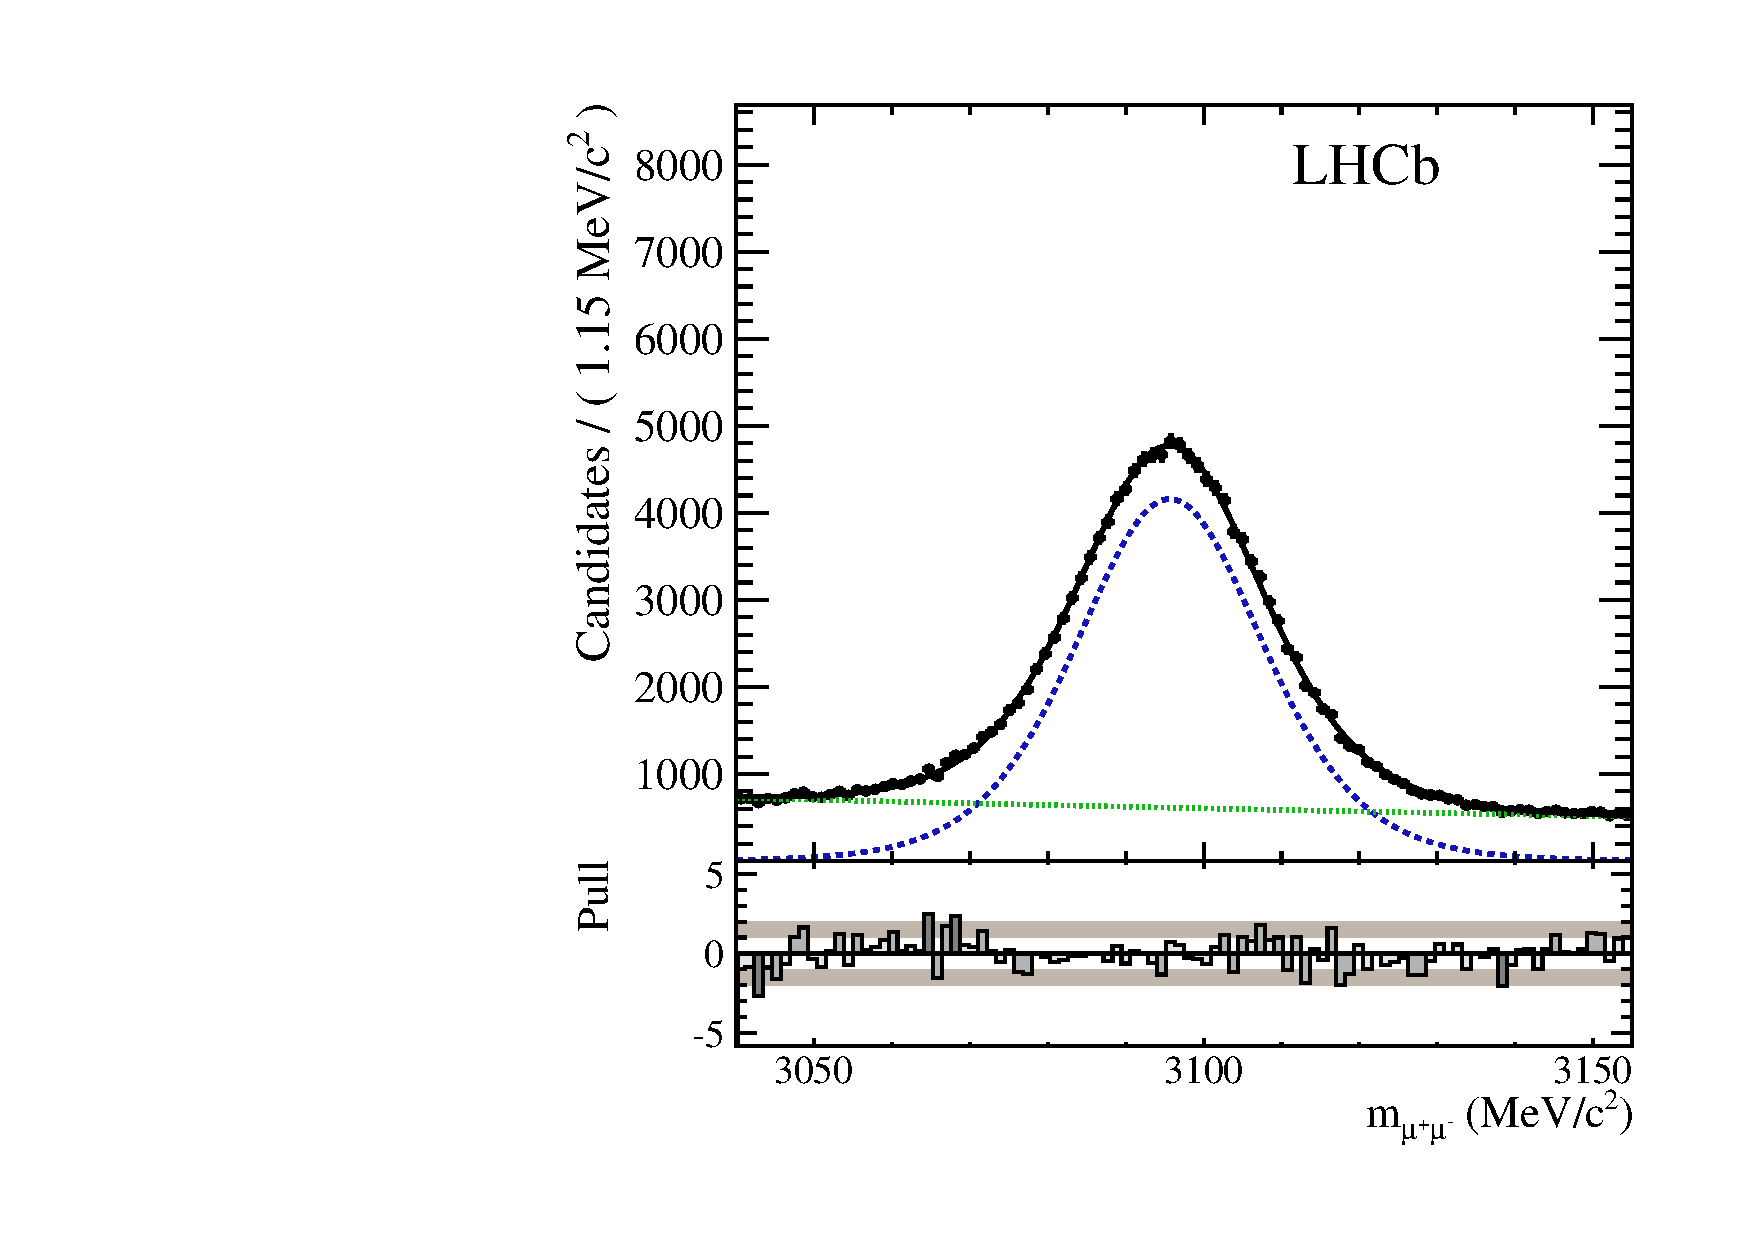
\includegraphics[width=0.49\textwidth]{private/content/measurement-of-sin2beta/figs/resolution_mass_jpsi_ll.pdf}
\label{fig:measurement_of_sin2beta:resolution_and_acceptance:resolution:jpsi_mass}
\caption{Invariant $\Jpsi$ candidate mass distribution in the (left) \catDD and
(right) \catLL subsample. Data are shown in black, the projection of the total
\acs{PDF} as solid black line, the signal component described by an Ipatia
\acs{PDF} as dashed blue line, and the exponential background component as
dotted green line.}
\end{figure}
%



% ------------------------------------------------------------------------------
\subsection{Decay time acceptance}
\label{sec:measurement_of_sin2beta:resolution_and_acceptance:acceptance}

Acceptance effects that alter the distribution of the decay time might result
from selection requirements or inefficiencies in the event reconstruction.
\Cref{sec:measurement_of_sin2beta:resolution_and_acceptance:acceptance:lower}
summarises acceptance effects stemming from lifetime biasing selection cuts from
the trigger requirements
(\cf \cref{sec:measurement_of_sin2beta:data_preparation:trigger}). Reconstruction
inefficiencies mainly caused by the \VELO track reconstruction algorithms (\cf
\cref{sec:lhcb_experiment:tracking}) are outlined in
\cref{sec:measurement_of_sin2beta:resolution_and_acceptance:acceptance:upper}.

% ..............................................................................
\subsubsection{Trigger induced decay time acceptance}
\label{sec:measurement_of_sin2beta:resolution_and_acceptance:acceptance:lower}

The biased trigger lines (\cf
\cref{sec:measurement_of_sin2beta:data_preparation:trigger}) and the stripping
cut on the reconstructed decay time of the $\Bd$ candidates result in a non-flat
acceptance.

In order to correctly describe these effects, the data sample is split into two
disjoint categories of candidates that show a substantially different behaviour
regarding their decay time acceptance. All candidates passing the \emph{almost
unbiased} (\textbf{\catAU}) trigger requirements show nearly no decay time
acceptance effects, in contrast to the sample of candidates passing the
\emph{exclusively biased} (\textbf{\catEB}) trigger requirements. The addressed
requirements are:
%
\begin{description}
  \item[\catAU] \TriggerReqAU
  \item[\catEB] \TriggerReqEB
\end{description}
%
To construct the acceptance in terms of ratios, a sample of candidates that pass
a set of unbiased trigger requirements is needed:
%
\begin{description}
  \item[Unbiased] \TriggerReqUB
\end{description}
%
The acceptance of the \catAU subsample can be computed using the overlap of events
which pass both the \HLTTwoDiMuonDetachedJpsi and the
\HLTTwoDiMuonJpsi line. Both lines are using the same trigger cuts except for
an additional cut on the flight distance significance (see
\cref{tab:measurement_of_sin2beta:data_preparation:trigger:hlt2:cuts}) in the
case of the biased lines. The acceptance can then be written as a time-dependent
efficiency $\varepsilon_\text{\catAU}$, with
%
\begin{equation}
  \begin{split}
    \varepsilon_\text{\catAU} &= \frac{\VerbAU \VerbAnd \HLTTwoDiMuonJpsi}{\VerbUB}\\
                              &= \frac{\TriggerReqAUEnumerator}{\TriggerReqUB}.
  \end{split}
\end{equation} 
%
For the \catEB subsample, there is no corresponding reference sample available, so
strictly speaking we cannot construct a true efficiency. Nonetheless, the ratio
of the \catEB subsample and the unbiased subsample can be computed as
$\varepsilon_\text{\catEB}$.
%
\begin{equation}
  \begin{split}
    \varepsilon_\text{\catEB} &= \frac{\VerbEB}{\VerbUB}\\
                              &= \frac{\TriggerReqEB}{\TriggerReqUB}
  \end{split}
\end{equation}
%
In other words $\varepsilon_\text{\catAU}$ quantifies the efficiency due to the
\HLTTwoDiMuonDetachedJpsi requirement, whereas $\varepsilon_\text{\catEB}$
effectively quantifies the relative efficiency due to the \HLTOneTrackMuon
requirement.

\subsubsection*{Methodology}
% \label{sec:propertime:methodology}

The data set for studying the trigger acceptance effects consists of all events
that are selected by the \StrippingDetached stripping line and pass the
offline selection. As the tagged and untagged candidates are expected to behave
equally concerning the studied effect all available candidates are used.
On the remaining multiple candidates, a random candidate selection is applied.
All candidates are selected by one of the following trigger lines:
\HLTOneDiMuonHighMass, \HLTOneTrackMuon, \HLTTwoDiMuonJpsi, or
\HLTTwoDiMuonDetachedJpsi.

The efficiencies are time-dependent and, since the focus lies on the the
acceptance of the signal decay time distribution, have to be determined through
a fit. To do so, a simultaneous fit for the signal yield is performed in ten
bins of decay time. The bin boundaries are chosen in a way that each bin
contains the same number of events (before splitting the data into the different
fit categories). The fit is also performed simultaneously in categories of track
type, tagger, and both trigger sets given by the numerators of
$\varepsilon_\text{\catAU}$ and $\varepsilon_\text{\catEB}$. The yields for the
different tagger and track type categories are summarized (including error
propagation). Then the efficiency per time bin is calculated. For
$\varepsilon_{\catAU}$ a binomial error is estimated, while a Gaussian error
propagation is used for $\varepsilon_{\catEB}$.

In the mass fit, the signal peak is described by a double Gaussian with a shared
mean, while a single exponential is used to describe the combinatorial
background. \Cref{fig:measurement_of_sin2beta:resolution_and_acceptance:acceptan
ce:lower:mass_fits} shows both mass distributions and fit projections for the
biased and unbiased sample, respectively. In both plots the sum over all
categories is displayed.
%
\begin{figure}
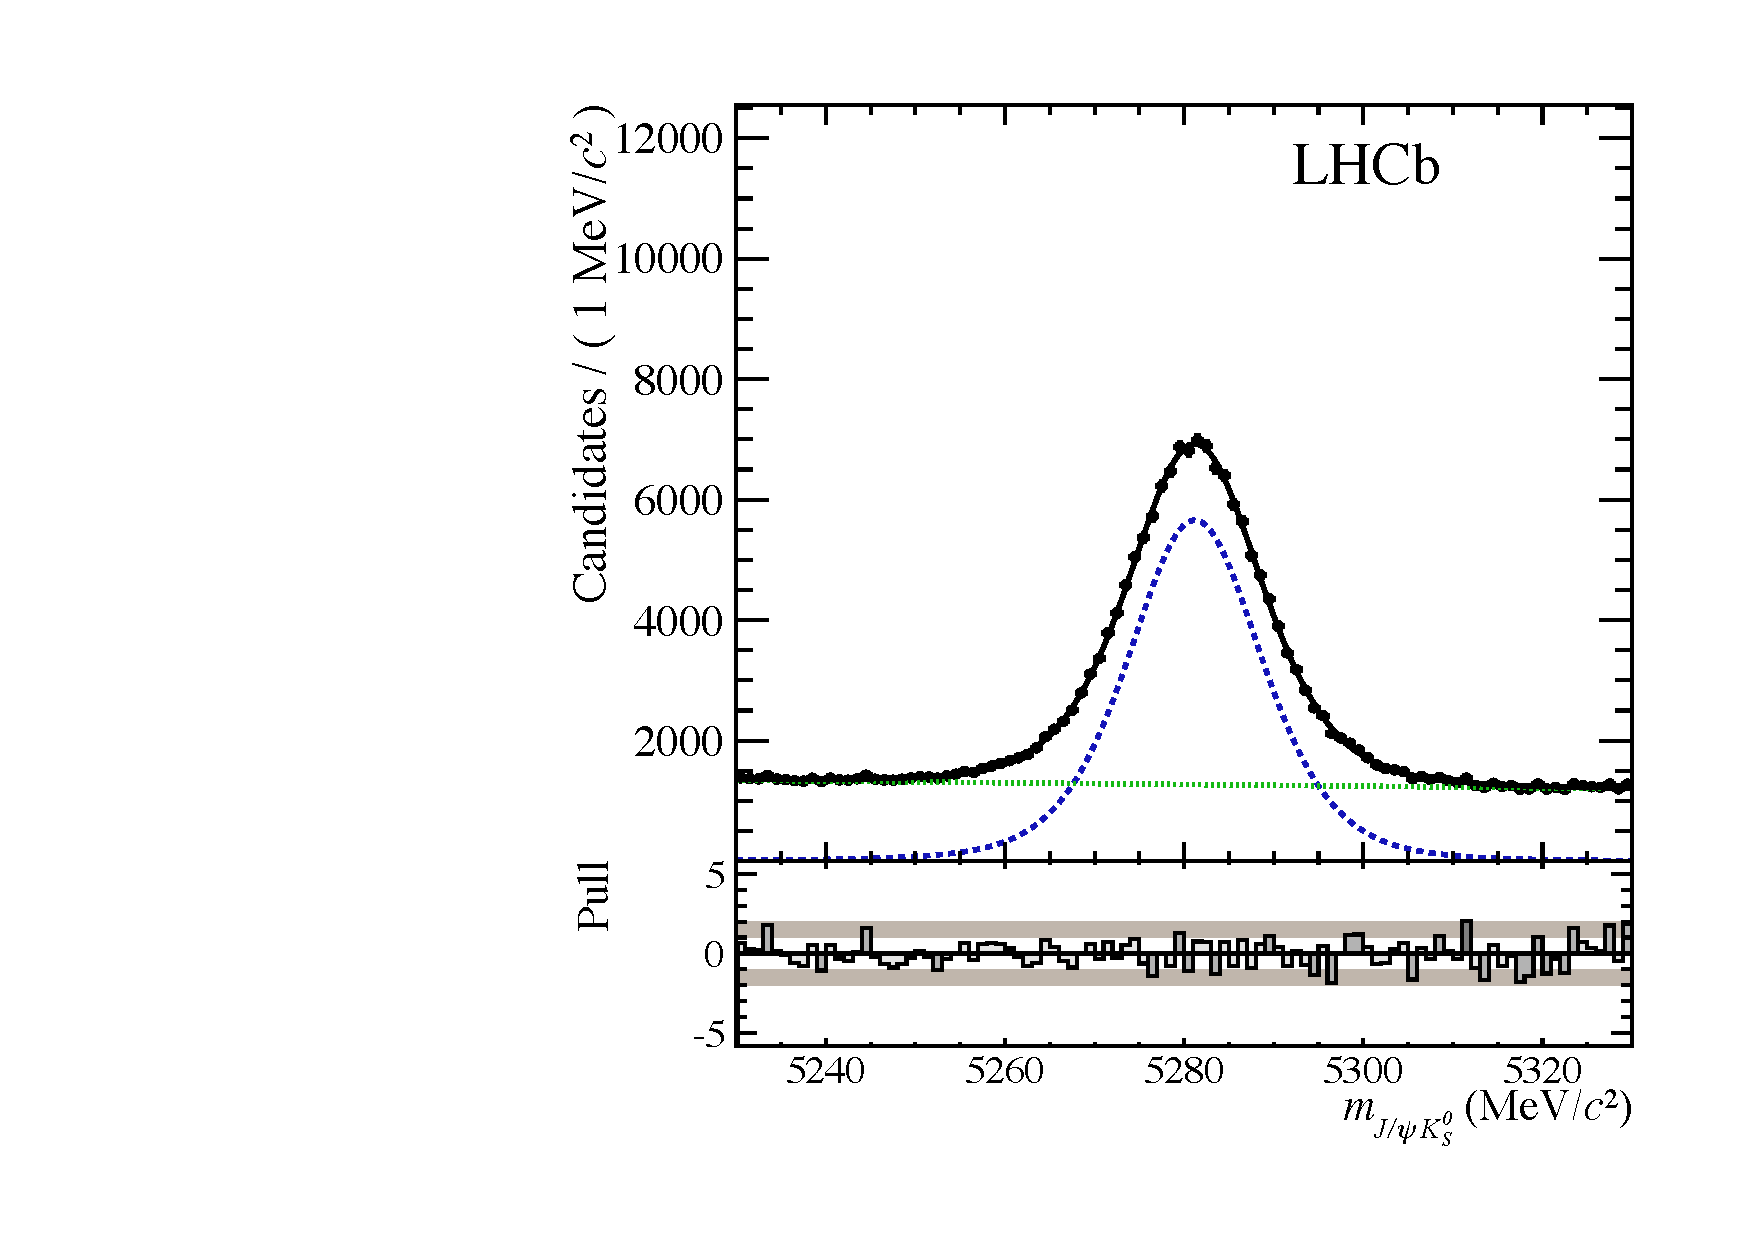
\includegraphics[width=0.49\textwidth]{private/content/measurement-of-sin2beta/figs/mass_trigger_efficiency_biased.pdf}
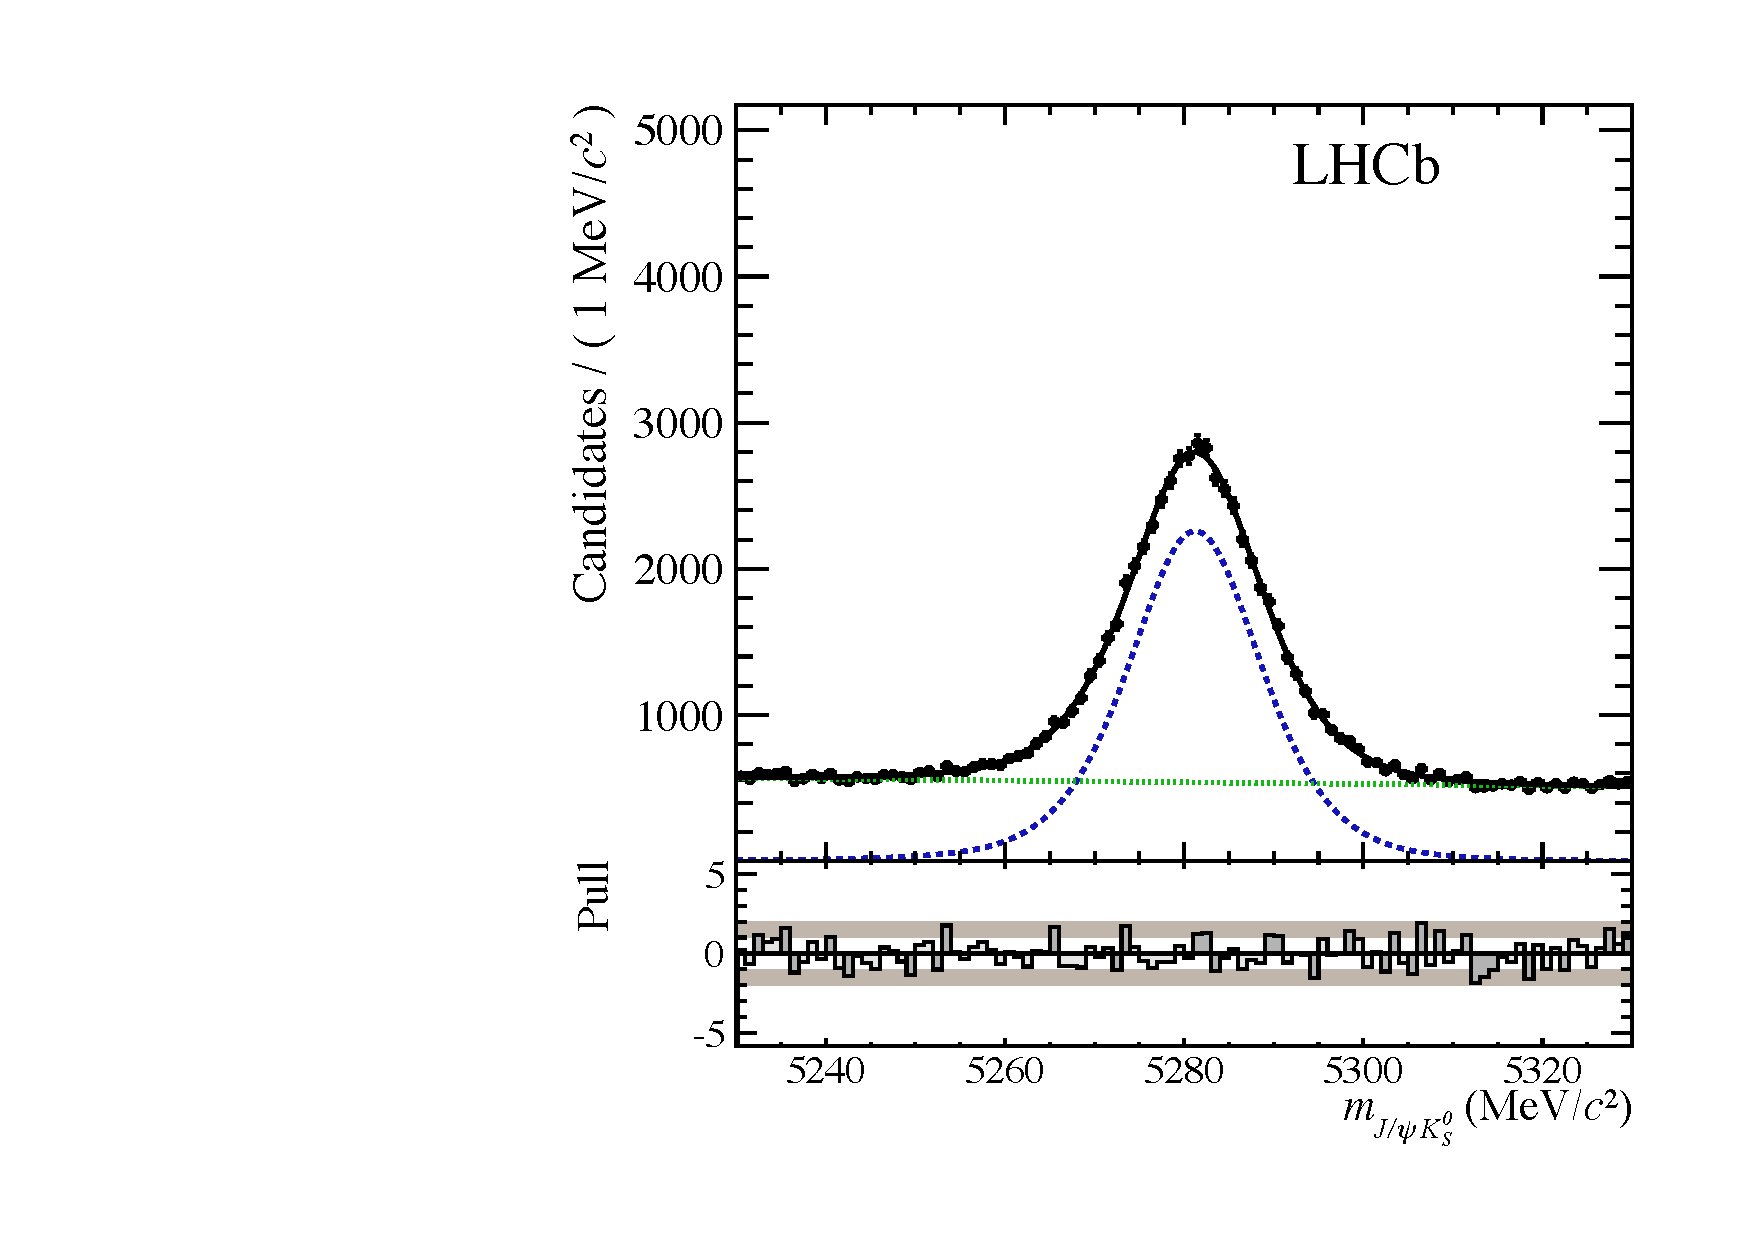
\includegraphics[width=0.49\textwidth]{private/content/measurement-of-sin2beta/figs/mass_trigger_efficiency_unbiased.pdf}
\label{fig:measurement_of_sin2beta:resolution_and_acceptance:acceptance:lower:mass_fits}
\caption{Mass distribution and fit projection summarised over all categories for
the (left) biased (\catAU and \catEB) and the (right) unbiased sample.}
\end{figure}
%
\Cref{fig:measurement_of_sin2beta:resolution_and_acceptance:acceptance:lower:splines} 
shows the acceptance histograms for the almost unbiased and the exclusively
biased sample. In the nominal fit we use cubic splines\addref{Cubic splines}
instead of the histograms themselves. Each bin centre is used as a knot for the
splines. The bin contents determine the shape of the splines. However, the bin
contents aren't fixed but constrained with a Gaussian function where the width
is given by the uncertainty on the bin content. As there is no information about
the acceptance at the decay time limits, the efficiency is assumed to be flat
between the lower decay time limit at \SI{0.3}{\ps} and the first bin
centre/knot and the last bin centre/knot and the upper decay time limit at
\SI{18.3}{\ps}, respectively.
%
\begin{figure}
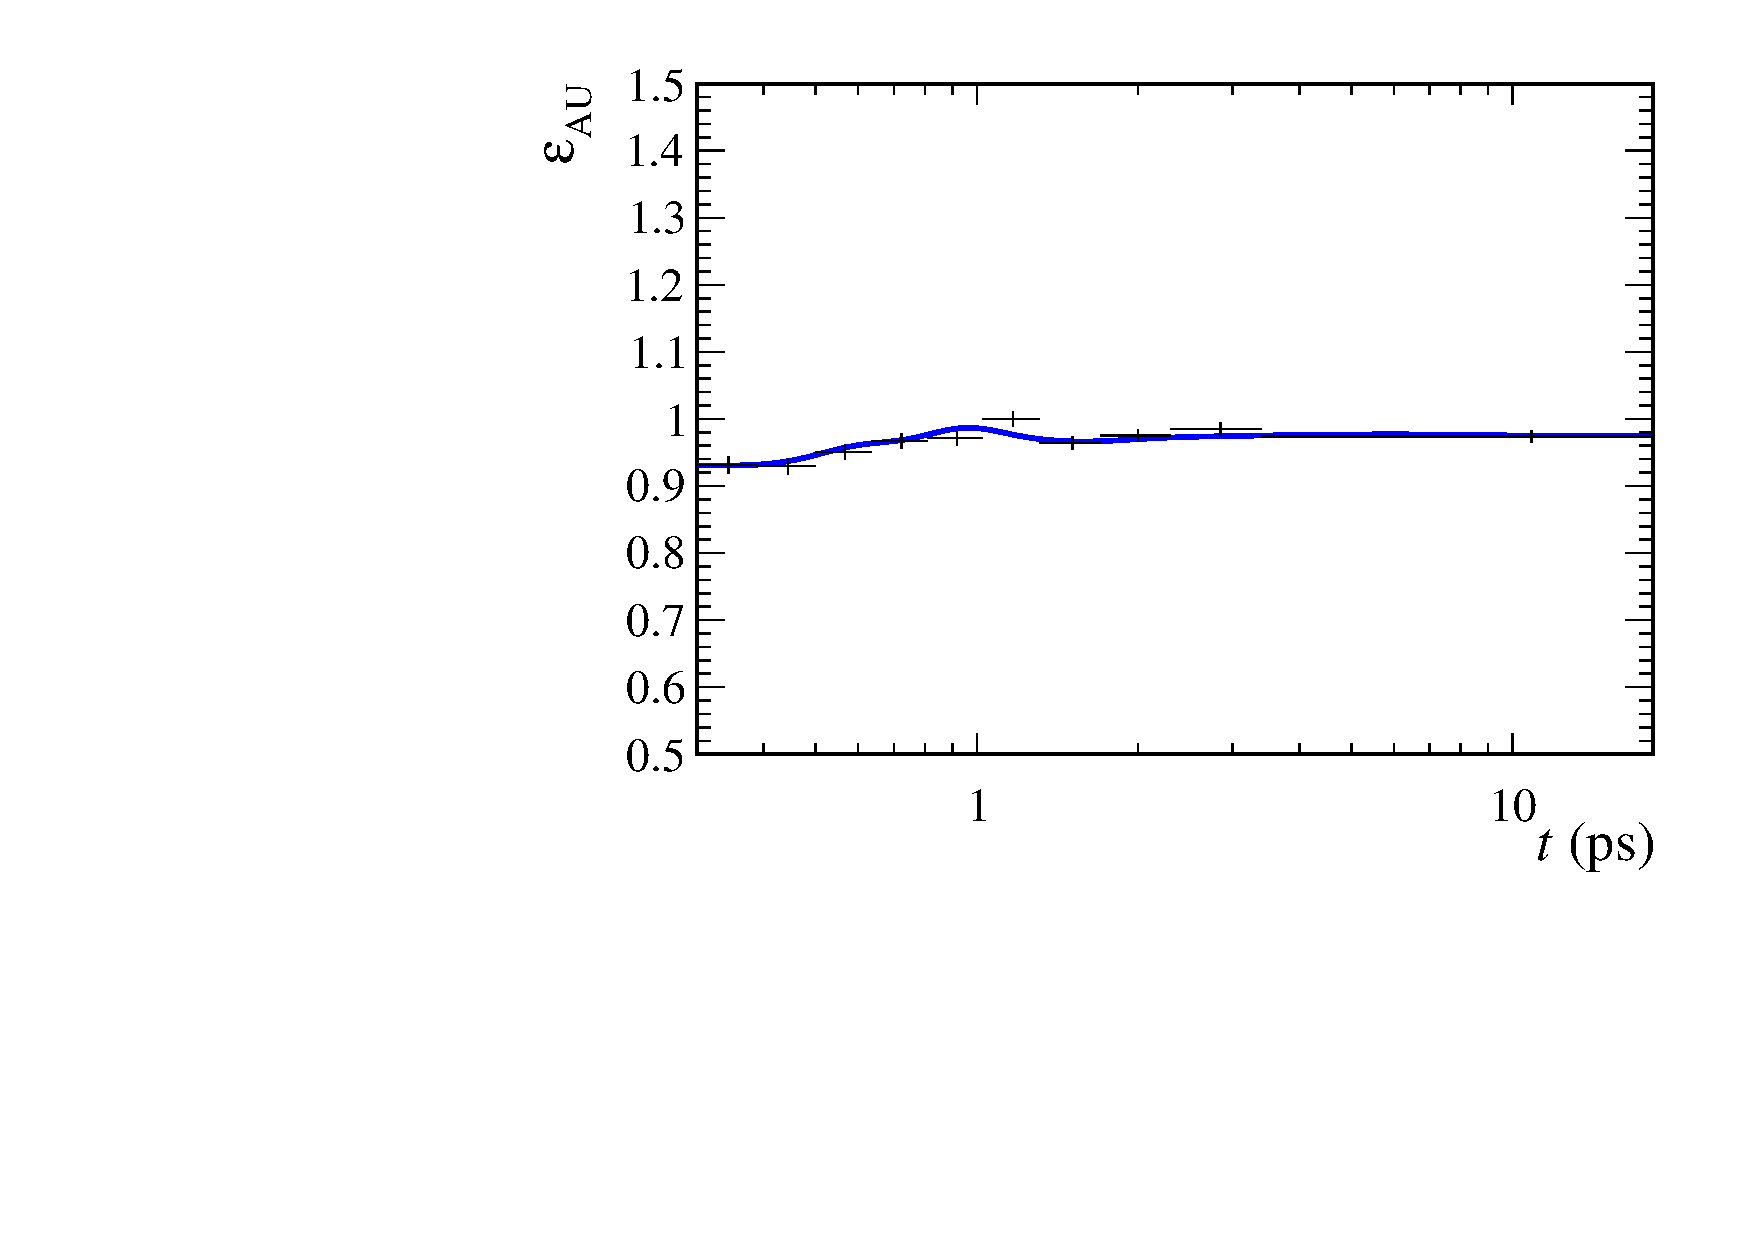
\includegraphics[width=0.49\textwidth]{private/content/measurement-of-sin2beta/figs/trigger_acceptance_spline_AU.pdf}
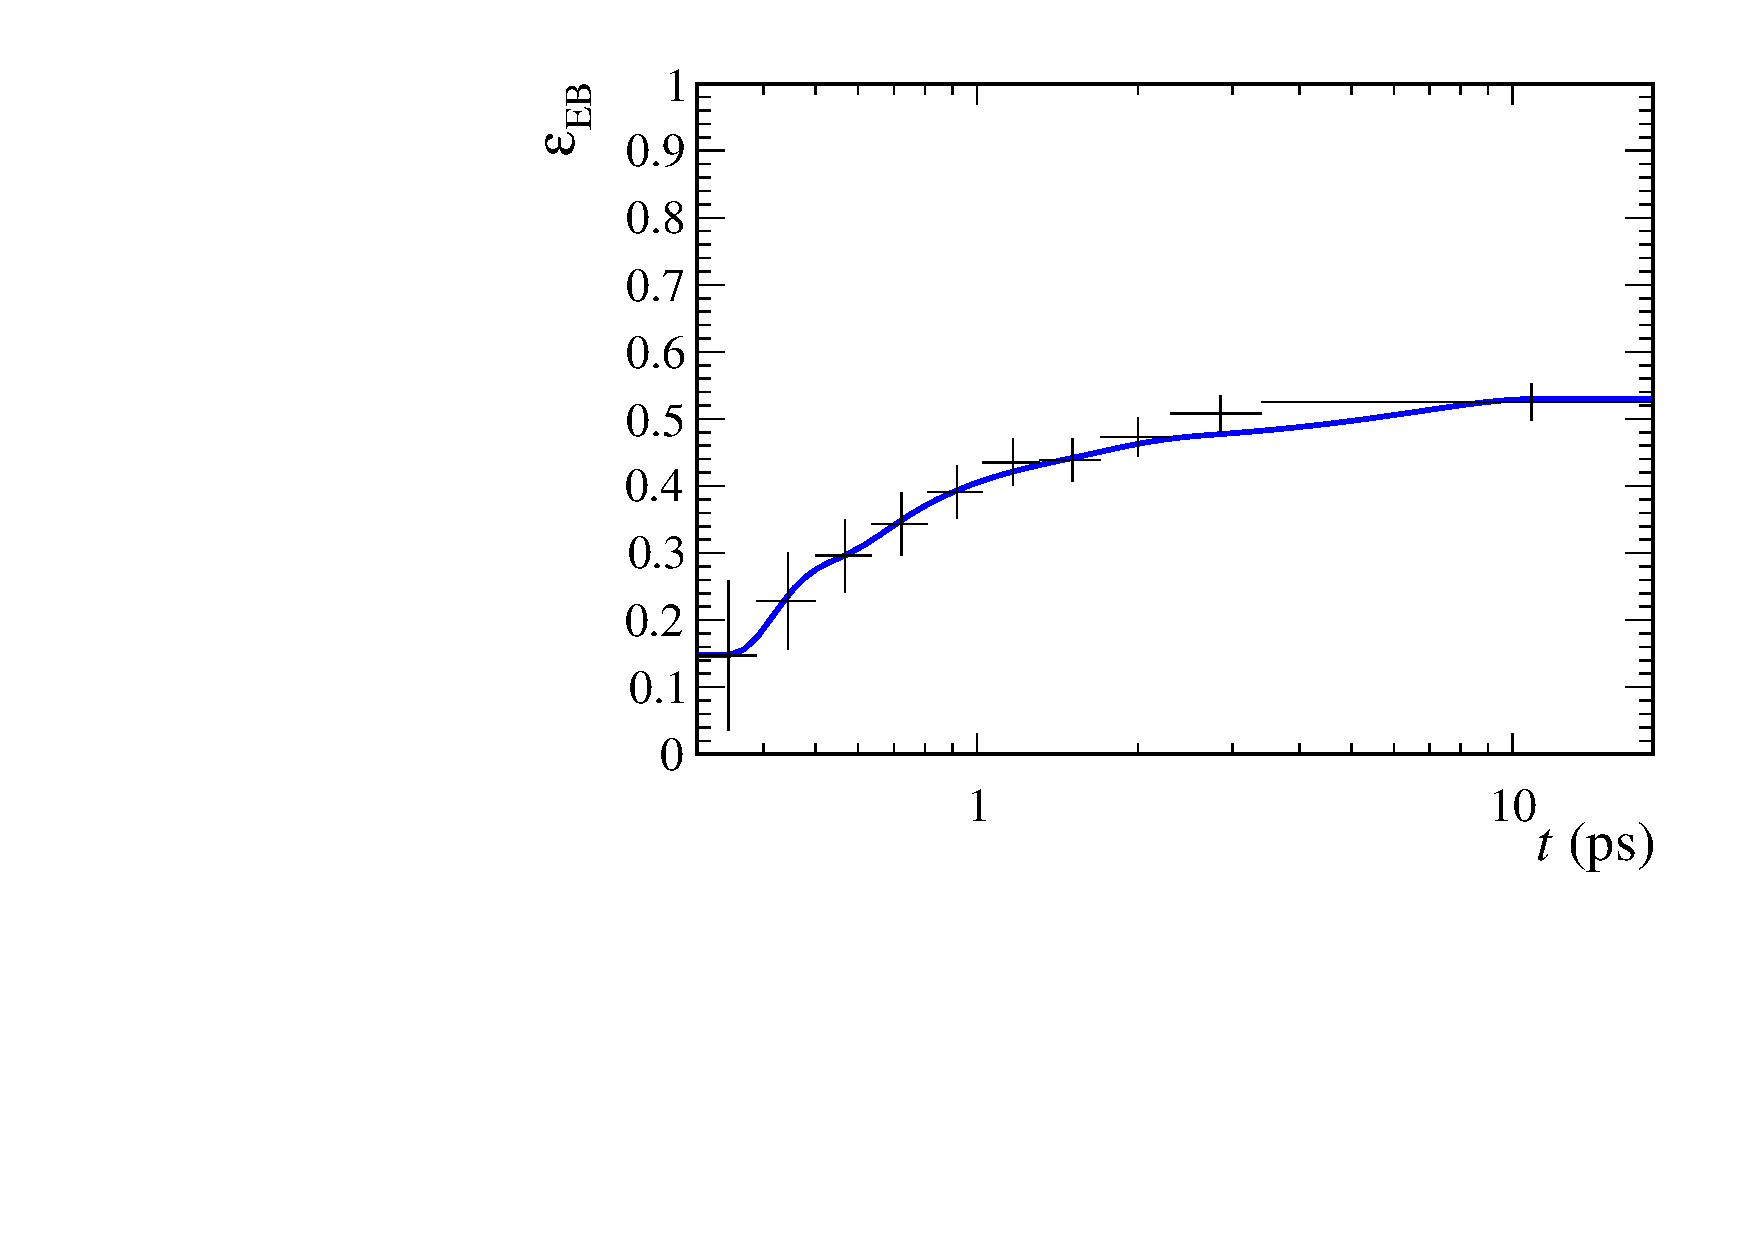
\includegraphics[width=0.49\textwidth]{private/content/measurement-of-sin2beta/figs/trigger_acceptance_spline_EB.pdf}
\label{fig:measurement_of_sin2beta:resolution_and_acceptance:acceptance:lower:splines}
\caption{Histograms of the trigger acceptance for the (left) almost unbiased and
the (right) exclusively biased sample. The blue curve shows the fitted
acceptance using cubic splines.}
\end{figure}

% ..............................................................................
\subsubsection{Upper decay time acceptance}
\label{sec:measurement_of_sin2beta:resolution_and_acceptance:acceptance:upper}

Due to the \VELO reconstruction inefficiency\todo{Be more precise, FastVelo
algorithm} and other reconstruction and selection effects, a decay time
acceptance is observed for events with larger decay times. To account for
this effect a correction factor $\beta_\tau$ is included into the fit model
using the modified lifetime
%
\begin{equation}
  \widetilde{\tau} = \frac{\tau}{1 + \beta_\tau \tau} ,
\end{equation}
%
which expands to
%
\begin{equation}\label{eq:measurement_of_sin2beta:resolution_and_acceptance:acceptance:upper:linear}
\begin{split}
  \Prob{}{}\left(t\right) &= \exponential{-\frac{t}{\tau}\left(1+\beta_{\tau}\tau\right)} \\
                          &= \exponential{-\frac{t}{\tau}-\beta_{\tau}t} = \exponential{-\frac{t}{\tau}} \exponential{-\beta_{\tau}t} \\
                          &= \exponential{-\frac{t}{\tau}}\left(1-\beta_{\tau} t+\frac{\beta_{\tau}^2 t^2}{2}+\order{\left((\beta_{\tau} t)^3\right)}\right).
\end{split}
\end{equation}
%
The value of $\beta_\tau$ is determined using a fit to simulated data while
fixing the lifetime $\tau$ to its generation value. Based on the
\BdToJpsiKS signal \MC data set, only candidates passing the
\StrippingPrescaled stripping line and the unbiased trigger lines
\HLTOneDiMuonHighMass and \HLTTwoDiMuonJpsi are chosen to avoid any
additional lifetime bias for events with short decay times. Only candidates
being matched on \MC as true signal events are considered. The nominal offline
selection is applied and from the remaining multiple (\acs{PV},\Bd) candidate pairs,
one is chosen randomly. To avoid wrong-\acs{PV} associations of the reconstructed
\BdToJpsiKS candidate the true \MC decay time is used in the fit. To reduce the
statistical uncertainties and no deviations of the decay time distributions are
expected all untagged events are included in this study. The number of remaining
\MC candidates available for this study is roughly \num{60000}. Due to
differences in the reconstruction efficiency the $\beta_\tau$ factor is
determined separately for \catOO/\catOT and \catDD/\catLL events
(\cref{tab:measurement_of_sin2beta:resolution_and_acceptance:acceptance:upper}).
%
\begin{table}
  \centering
  \caption{Decay time correction factor $\beta_\tau$ in \si{\per\pico\second}.}
  \begin{tabular}{ccc}
    \toprule
     & 2011 & 2012 \\
    \midrule
    downstream & $0.0036\pm0.0029$ & $0.0084\pm0.0032$ \\
    long track & $0.018\pm0.004$   & $0.035\pm0.005$ \\
    \bottomrule
  \end{tabular}
  \label{tab:measurement_of_sin2beta:resolution_and_acceptance:acceptance:upper}
\end{table}

\subsubsection*{Influence of higher order effects}
\todo{Leave out this possibility?}
To check the influence of higher order terms, a quadratic correction function is
tested where the second order term has an own degree of freedom given by
$\gamma_\tau$,
%
\begin{equation}\label{eq:measurement_of_sin2beta:resolution_and_acceptance:acceptance:upper:quadratic}
  \Prob{}{}\left(t\right) = \exponential{-\frac{t}{\tau}}\left(1-\beta_\tau t+ \gamma_\tau t^2\right).
\end{equation}
%
Again the parameters $\beta_\tau$ and $\gamma_\tau$ are fitted while fixing the
lifetime $\tau$. In \cref{tab:measurement_of_sin2beta:resolution_and_acceptance:acceptance:upper:secondorder} 
the results are listed for \catOO/\catOT and \catDD/\catLL events. To visualise
the effect, the per-bin ratio of the decay time distributions of signal \MC
events to events generated from \ToyMC is calculated and shown in
\cref{fig:measurement_of_sin2beta:resolution_and_acceptance:acceptance:upper}.
The \ToyMC decay time distribution follows an exponential function with the same
lifetime as used in the generation of the signal \MC. As the uncertainties on
$\beta_\tau$ and $\gamma_\tau$ are large and the parameters are strongly
correlated ($\rho>\SI{90}{\percent}$) we stick to the linear model. A possible
bias due to this choice is investigated in
\cref{sec:measurement_of_sin2beta:systematics:systematics:acceptance}.
%
\begin{table}
  \centering
  \caption{Decay time correction factors $\beta_\tau$ (in \si{\per\pico\second})
  and $\gamma_\tau$ (in \si{\per\square\pico\second}).}
  \label{tab:measurement_of_sin2beta:resolution_and_acceptance:acceptance:upper:quadratic}
  \begin{tabular}{ccccc}
    \toprule
     & \multicolumn{2}{c}{2011} & \multicolumn{2}{c}{2012} \\
     & $\beta_\tau$ & $\gamma_\tau$ & $\beta_\tau$ & $\gamma_\tau$ \\
    \midrule
    \catDD & $-0.016\pm0.007$ & $-0.0030\pm0.0008$ & $-0.001\pm0.007$         & $-0.0014\pm0.0009$\\ 
    \catLL & $-0.001\pm0.009$ & $-0.0028\pm0.0012$ & $\phantom{+}0.01\pm0.06$ & $-0.0027\pm0.0008$\\ 
    \bottomrule
  \end{tabular}
\end{table}
%
\begin{figure}
  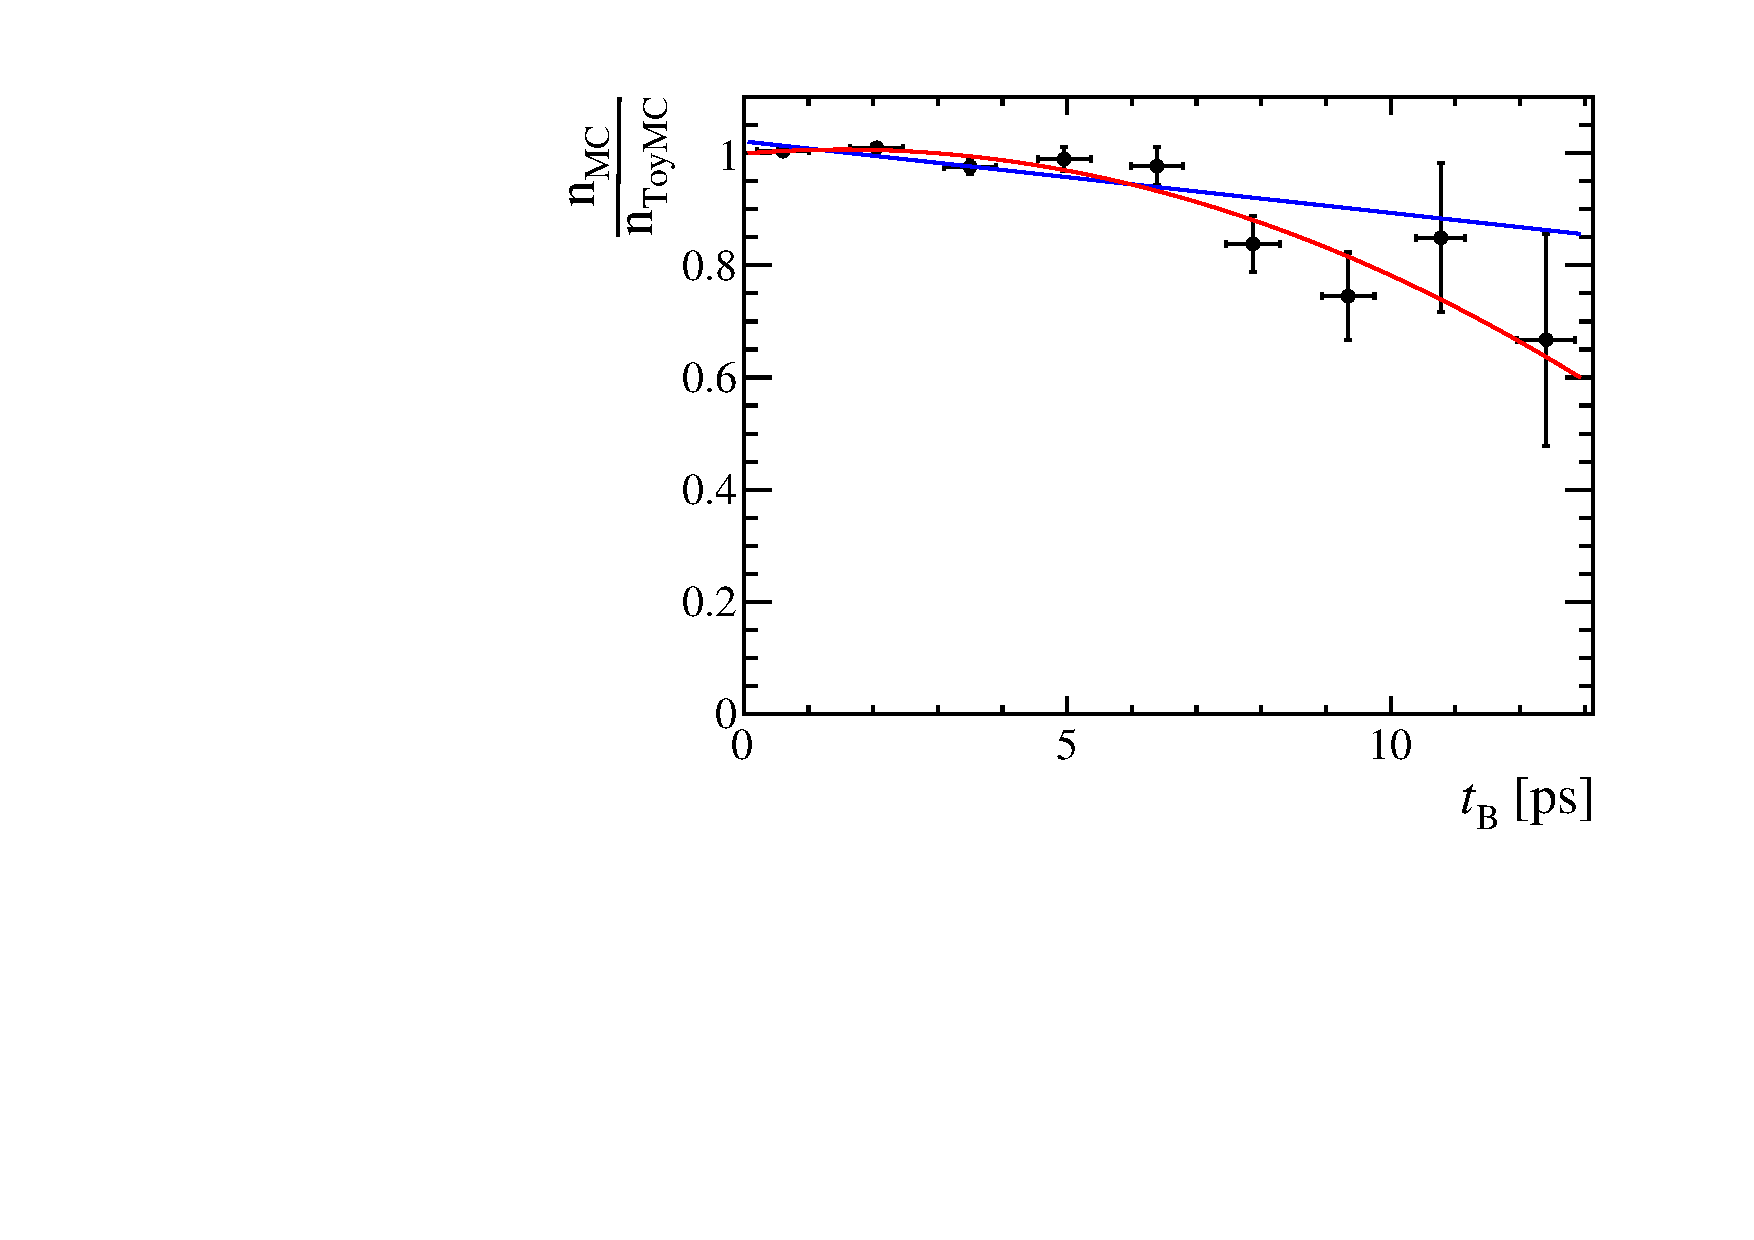
\includegraphics[width=0.49\textwidth]{private/content/measurement-of-sin2beta/figs/velo_acceptance_11_DD.pdf}\hfill
  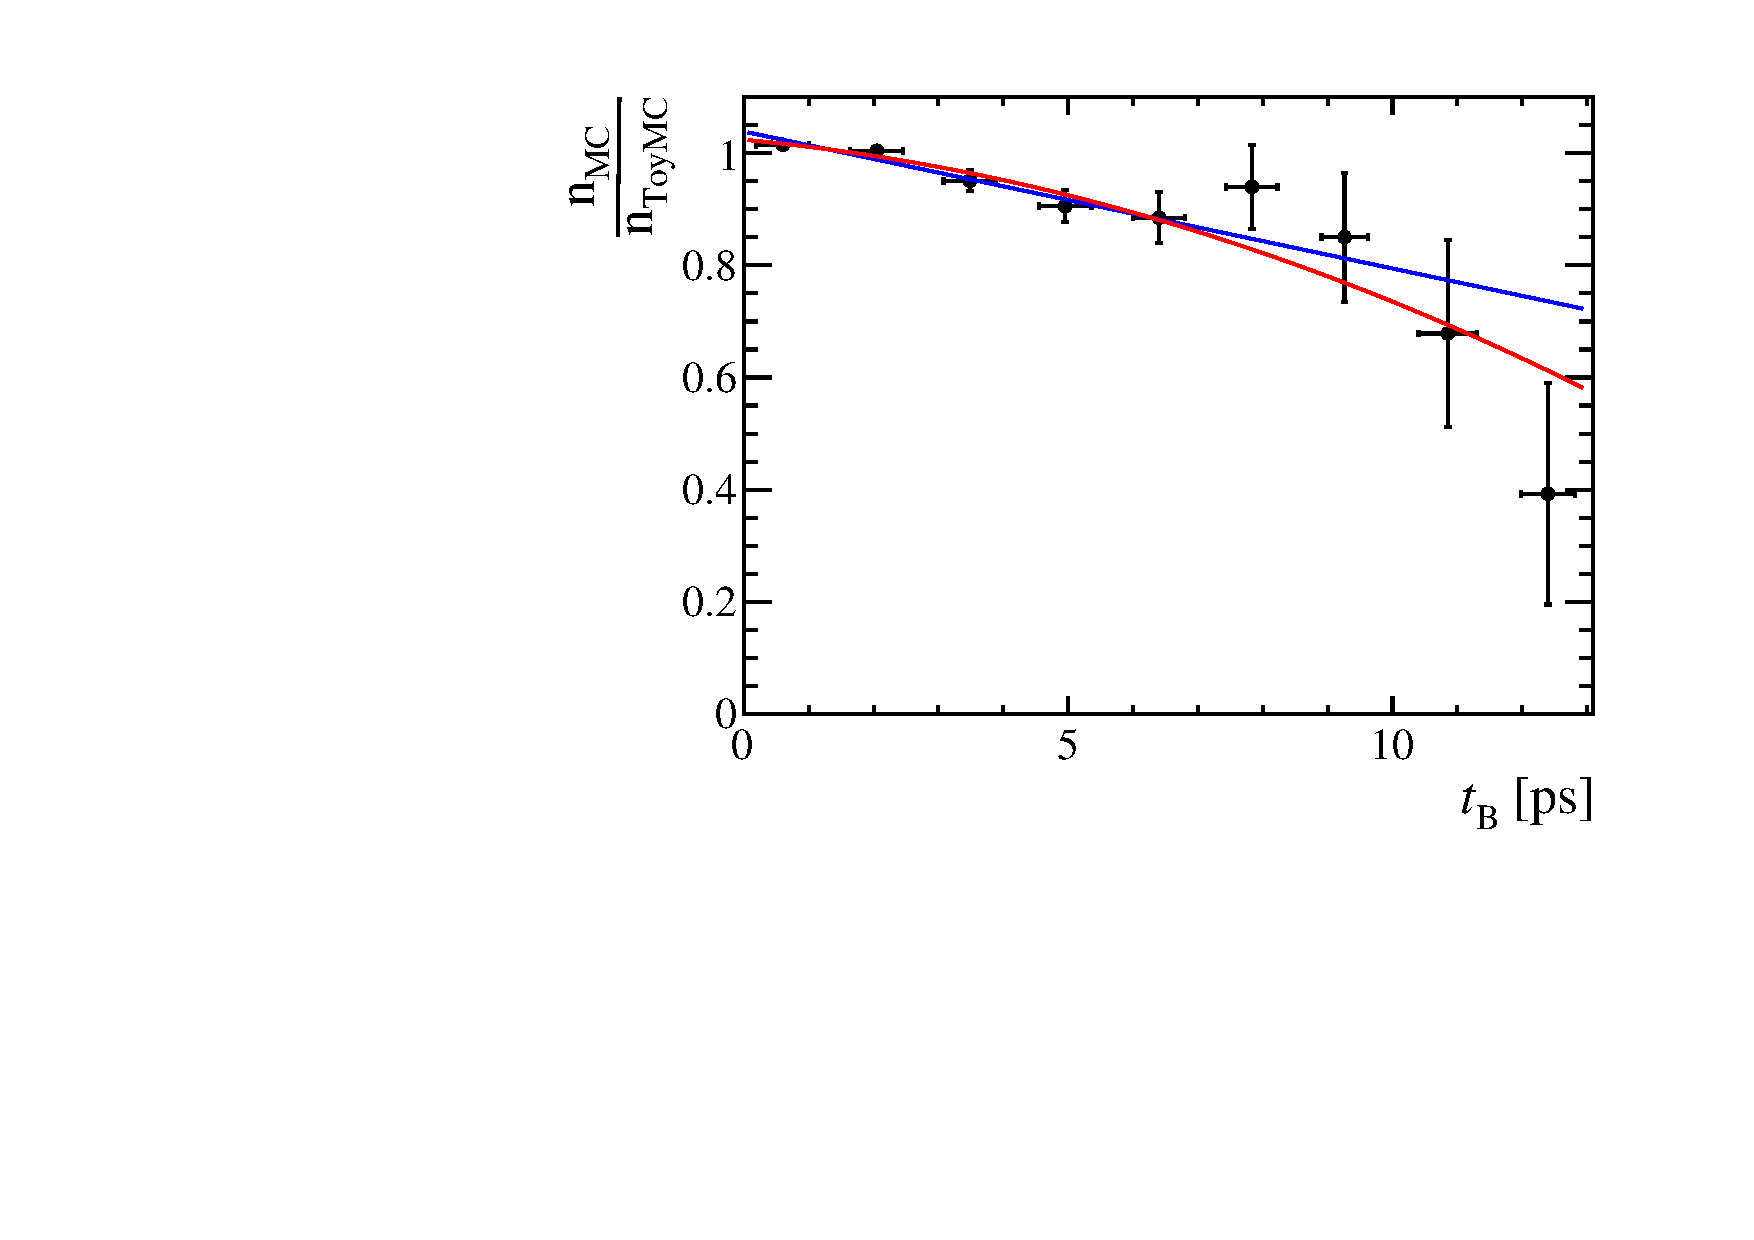
\includegraphics[width=0.49\textwidth]{private/content/measurement-of-sin2beta/figs/velo_acceptance_11_LL.pdf}
  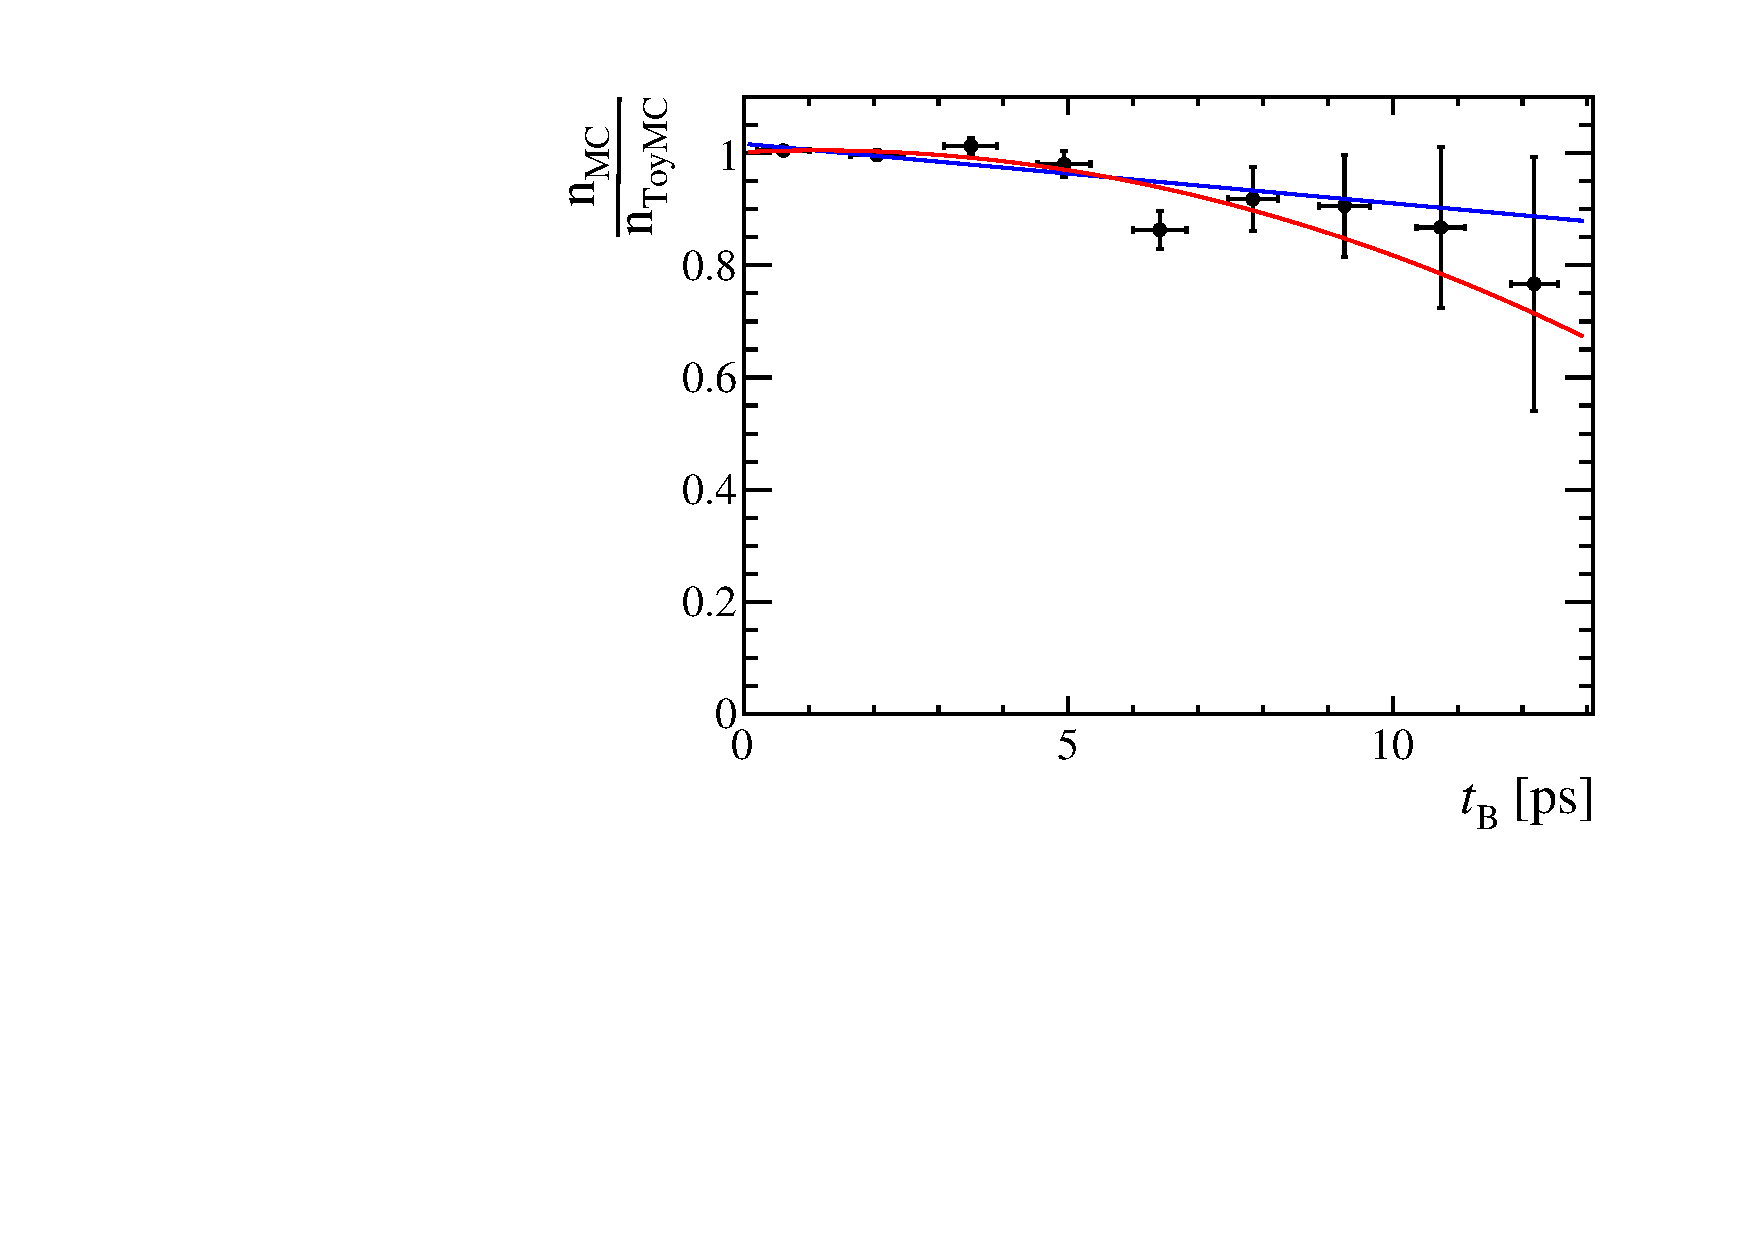
\includegraphics[width=0.49\textwidth]{private/content/measurement-of-sin2beta/figs/velo_acceptance_12_DD.pdf}\hfill
  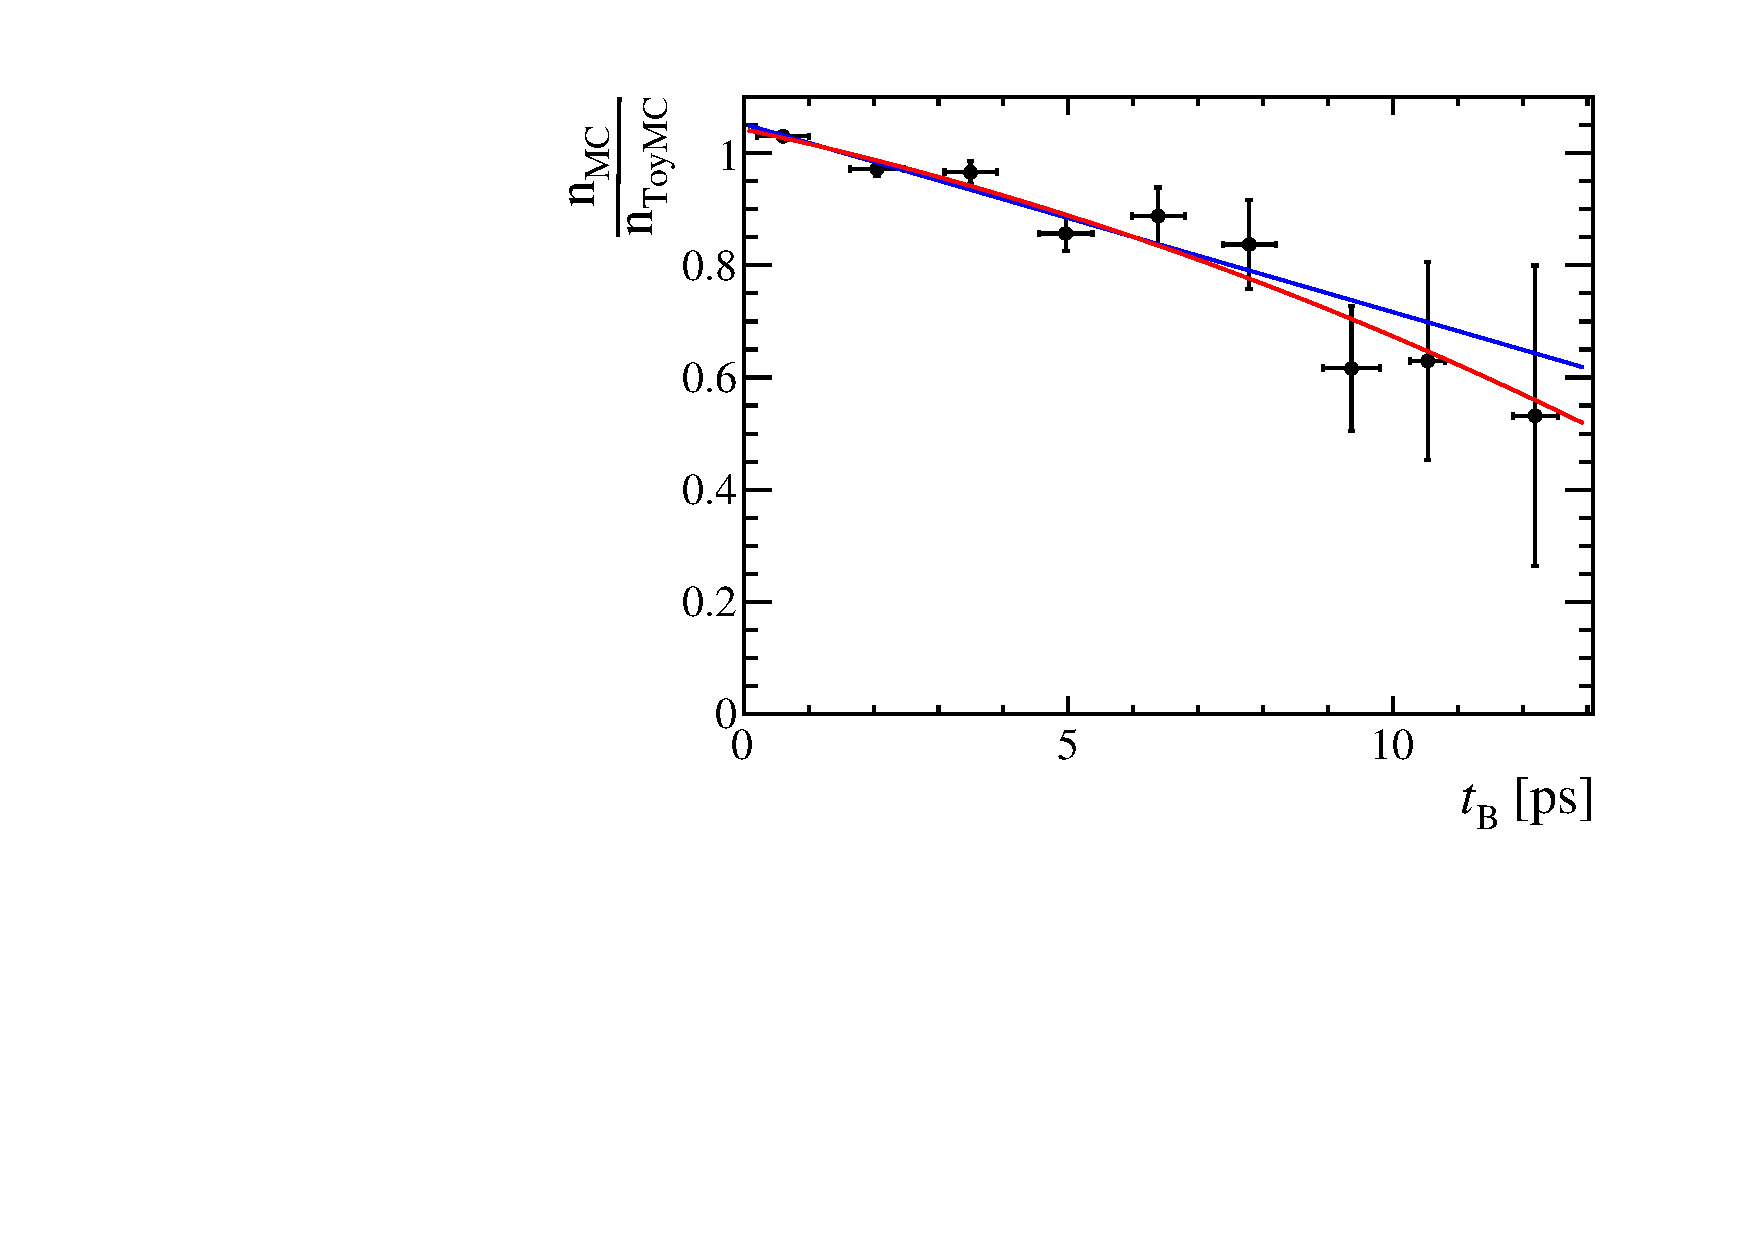
\includegraphics[width=0.49\textwidth]{private/content/measurement-of-sin2beta/figs/velo_acceptance_12_LL.pdf}
\caption{
Decay time ratio in bins of decay time for (left/right) \catDD/\catLL and
(top/bottom) \catOO/\catOT. The blue (red) curve shows a linear (quadratic) fit
to the data points.}
\label{fig:measurement_of_sin2beta:resolution_and_acceptance:acceptance:upper}
\end{figure}

\FloatBarrier

% %%%%%%%%%%%%%%%%%%%%%%%%%%%%%%%%%%%%%%%%%%%%%%%%%%%%%%%%%%%%%%%%%%%%%%%%%%%%%%
%!TEX root = ../../common/main.tex

\section{Likelihood fit}
\label{sec:measurement_of_sin2beta:likelihood_fit}

This section presents the model developed to describe the data and estimate the
values and uncertainties of the physics observables using an \uEML fit. Starting
with a short review of the \uEML method, the \acp{PDF} in use to describe the
different dimensions and components is shown, and the fit model is outlined.

The \CP observables of interest \SJpsiKS and \CJpsiKS are estimated in a
multi-dimensional simultaneous \uEML fit. As summarised in
\cref{tab:measurement_of_sin2beta:data_preparation:observables} the seven
observables $\vec{x}$ are given by the reconstructed mass and decay time of the
\Bd candidate, its decay time estimate, and its \OS and \SSpi tag decision as
well as the corresponding mistag estimates
%
\begin{equation}\label{eq:measurement_of_sin2beta:likelihood_fit:observables}
  \vec{x} = (\obsMass, \obsTime, \obsTimeError, \obsTagOS, \obsTagSS, \obsEtaOS, \obsEtaSS)\eqpd  
\end{equation}
%
The extended likelihood for a total of $N$ observed events in $j$ subsamples of
data, where $n=\sum_j n_j$, is then defined as
%
\begin{equation}\label{sec:measurement_of_sin2beta:likelihood_fit:uEML}
  \Likelihood{}{}\left(\vec{\theta},\vec{n};\vec{x}\right) = \frac{\exponential{-N} N^n}{n!} \prod_j \prod_{i=1}^{n_j} n_j \Prob{j}{}\left(\vec{x}_i;\vec{\theta}\right)\eqcm
\end{equation}
%
where $\vec{n}$ is the numbers of events, and $\vec{\theta}$ the parameters with
unknown values to be estimated by the \uEML fit. \important{Check definition of uEML}

\subsection{\acp{PDF} used in this analysis}
\label{sec:measurement_of_sin2beta:likelihood_fit:pdfs}

\subsubsection{Exponential}
\begin{equation}
  \Prob{\text{Exponential}}{}(x, \alpha) = \exponential{\alpha x}
\end{equation}

\subsubsection{Decay}
\begin{equation}
  \Prob{\text{Decay}}{}(x, \alpha) = \exponential{- \frac{x}{\alpha}}
\end{equation}

\subsubsection{Gaussian}
\begin{equation}
  \Prob{\text{Gaussian}}{}(x, \mu, \sigma) = \frac{1}{\sigma\sqrt{2\pi}}\exponential{-\frac{1}{2} \left(\frac{x-\mu}{\sigma}\right)^2}
\end{equation}

\subsubsection{Lognormal}
\begin{equation}
  \Prob{\text{Lognormal}}{}(x, \mu, k) = \frac{1}{x \sqrt{2\pi} \log (k)} \exponential{-\frac{\log^2 \left(\sfrac{x}{\mu}\right)}{2 \log^2(k)}}
\end{equation}

\subsubsection{BDecay}
\begin{multline}
  \Prob{\text{BDecay}}{}(x;...) = \\ \exponential{- \frac{x}{\alpha}}\left( A \cosh (\DG x) + B \sinh (\DG x) + C \cos (\dm x) + D \sin (\dm x) \right)
\end{multline}

\subsubsection{Ipatia}
\begin{multline}
  \Prob{\text{Ipatia}}{}(x, \mu, \sigma, \lambda, \zeta, \beta, a_1, a_2, n_1, n_2) = \\
    \begin{cases}
    ...     & \text{if $-a_1 < \frac{x-\mu}{\sigma} < a_2$} \\
    ...     & \text{if $-a_1 > \frac{x-\mu}{\sigma}      $} \\
    ...     & \text{if $ a_2 < \frac{x-\mu}{\sigma}$} \\
  \end{cases}
\end{multline}

\newpage




% ------------------------------------------------------------------------------
\subsection{Fitter validation}
\label{sec:measurement_of_sin2beta:likelihood_fit:validation}

\FloatBarrier

% %%%%%%%%%%%%%%%%%%%%%%%%%%%%%%%%%%%%%%%%%%%%%%%%%%%%%%%%%%%%%%%%%%%%%%%%%%%%%%
%!TEX root = ../../common/main.tex

\section{CPV measurement}
\label{sec:measurement_of_sin2beta:cpv_measurement}

Utilising the likelihood model presented in
\cref{sec:measurement_of_sin2beta:likelihood_fit} an \acf{uEML} fit is performed
to the nominal data set (\cf
\cref{sec:measurement_of_sin2beta:data_preparation:datasamples}).  The
\MinuitTwo algorithm implemented in the \RooFit (v3.60) framework from \ROOT
v5.34/18 is used to minimise the negative log-likelihood function with the
\emph{minimize} routine and \emph{strategy 2}. \Minos is used for the estimation
of the (asymmetric) parameter errors.

% ------------------------------------------------------------------------------
\subsection{Constrained parameters}
\label{sec:measurement_of_sin2beta:cpv_measurement:constrained_parameters}

Several parameters are incorporated as external inputs. These parameters are
constrained using a Gaussian \PDF with the mean value fixed to the parameter's
value and the Gaussian's width to the uncertainty.
\Cref{tab:measurement_of_sin2beta:cpv_measurement:constrained_parameters} lists
the constrained parameters as well as the source of the value and its
uncertainty employed in the fit.

Individual production asymmetry values are used for the \catOO and \catOT
subsamples. Using the recent \LHCb measurement \cite{Aaij:2014bba} of the
production asymmetry as a function of the \acf{pT} and the \acf{pseudorapidity}
the per-\pT-\pseudorapidity-bin signal fractions $\varepsilon_i =
\sfrac{f_i}{\sum_i f_i}$ of the nominal dataset are determined to calculate a
weighted average of the production asymmetries
%
\begin{equation}
  A_P = \sum_i \varepsilon_i A_{P,i}\eqcm
\end{equation}
where $f_i$ is the number of signal candidates per bin and $A_{P,i}$ the
measured production asymmetry in bin $i$ taken from Ref.~\cite{Aaij:2014bba}.
This yields
%
\begin{equation}
  \begin{split}
    A_P^{\catOO} &= -0.0108 \pm 0.0052 \statp \pm 0.0014 \systp \eqcm \\
    A_P^{\catOT} &= -0.0104 \pm 0.0051 \statp \pm 0.0014 \systp \eqpd \\
  \end{split}
\end{equation}
%
As the measurement has been performed on $\SI{7}{\TeV}$ data only, the numbers for
$A_P^{11}$ and $A_P^{12}$ are highly correlated. We therefore
constraint $A_P^{11}$ in the fit and model $A_P^{12} = A_P^{11} +
\Delta A_P$ with $\Delta A_P = 0.0004 \pm 0.0018 \systp$, where
the systematic uncertainty accounts for the production asymmetry differences
observed for the two data-taking conditions in \LHCb{'s} recent measurement of
the semi-leptonic $\CP$ asymmetry~\cite{Aaij:2014nxa}.
%
\begin{table}
\caption{Parameters that are constrained in the fit.}
\label{tab:measurement_of_sin2beta:cpv_measurement:constrained_parameters}
\centering
\begin{tabular}{lr@{$\,\pm\,$}ll}
  \toprule
  Parameter                        & \multicolumn{2}{l}{Value and uncertainty} & Source \\
  \midrule
  $A_P^{\catOO}$                   & $-0.0108$ & $0.0052$  & \cite{Aaij:2014bba} \\
  $\Delta A_P$                     & $0.0004$  & $0.0018$  & \cite{Aaij:2014bba,Aaij:2014nxa} \\
  $\DMd$ (\si{\planckbar\per\ps})  & $0.510$   & $0.003$   & \cite{Agashe:2014kda} \\
  $\p{0}{\text{\acs*{OS}}}$        & $0.3815$  & $0.0011$  & \cref{eq:flavour_tagging:calibration:os:parameters} \\
  $\p{1}{\text{\acs*{OS}}}$        & $0.978$   & $0.012$   & \cref{eq:flavour_tagging:calibration:os:parameters} \\
  $\deltap{0}{\text{\acs*{OS}}}$   & $0.0148$  & $0.0016$  & \cref{eq:flavour_tagging:calibration:os:asymmetries} \\
  $\deltap{1}{\text{\acs*{OS}}}$   & $0.070$   & $0.018$   & \cref{eq:flavour_tagging:calibration:os:asymmetries} \\
  $\p{0}{\text{\acs*{SS}}}$        & $0.4232$  & $0.0029$  & \cref{eq:flavour_tagging:calibration:ss:parameters} \\
  $\p{1}{\text{\acs*{SS}}}$        & $1.011$   & $0.064$   & \cref{eq:flavour_tagging:calibration:ss:parameters} \\
  $\deltap{0}{\text{\acs*{SS}}}$   & $-0.0026$ & $0.0043$  & \cref{eq:flavour_tagging:calibration:ss:parameters} \\
  $\deltap{1}{\text{\acs*{SS}}}$   & $-0.17$   & $0.10$    & \cref{eq:flavour_tagging:calibration:ss:parameters} \\
  \bottomrule
\end{tabular}
\end{table}

% ------------------------------------------------------------------------------
\subsection{Fixed parameters}
\label{sec:measurement_of_sin2beta:cpv_measurement:fixed_parameters}

As mentioned before, various parameters are fixed in the nominal fit. These are
the mass parameters obtained on simulated data
(\cref{sec:measurement_of_sin2beta:cpv_measurement:fixed_parameters:mass}), the
parameters describing the distribution of the decay time error estimates (\cref{
sec:measurement_of_sin2beta:cpv_measurement:fixed_parameters:decay_time_error:sig,sec:measurement_of_sin2beta:cpv_measurement:fixed_parameters:decay_time_error:bkg}), 
the parameters of the cubic spline functions used to model the \OS and
\SSpi mistag estimate distributions (\cref{sec:measurement_of_sin2beta:cpv_measurement:fixed_parameters:eta:sig:os,sec:measurement_of_sin2beta:cpv_measurement:fixed_parameters:eta:bkg:os,sec:measurement_of_sin2beta:cpv_measurement:fixed_parameters:eta:sig:ss,sec:measurement_of_sin2beta:cpv_measurement:fixed_parameters:eta:bkg:ss}), 
the calibration parameters of the decay time resolution model (\cref{sec:measurement_of_sin2beta:cpv_measurement:fixed_parameters:decay_time_resolution}) 
and the parameters of the cubic spline functions utilised to parametrise
the shape of the lower decay time acceptance (\cref{sec:measurement_of_sin2beta:cpv_measurement:fixed_parameters:acc:au,sec:measurement_of_sin2beta:cpv_measurement:fixed_parameters:acc:eb})
%
\begin{table}
\caption{Fixed mass parameters.}
\label{sec:measurement_of_sin2beta:cpv_measurement:fixed_parameters:mass}
\centering
\begin{tabular}{lr@{$\,\pm\,$}l}
  \toprule
  Parameter                     & \multicolumn{2}{c}{Fixed Value} \\
  \midrule
  $\alpha_{1,m}^\text{\catDD}$      & \multicolumn{2}{c}{$2.28$}\\
  $\alpha_{1,m}^\text{\catLL}$      & \multicolumn{2}{c}{$2.1$}\\
  $\alpha_{2,m}^\text{\catDD}$      & \multicolumn{2}{c}{$2.08$}\\
  $\alpha_{2,m}^\text{\catLL}$      & \multicolumn{2}{c}{$2.43$}\\
  $\lambda_m^\text{\catDD}$         & \multicolumn{2}{c}{$-2.8$}\\
  $\lambda_m^\text{\catLL}$         & \multicolumn{2}{c}{$-3.6$}\\
  $\zeta_m^\text{\catDD}$           & \multicolumn{2}{c}{$0.0$}\\
  $\zeta_m^\text{\catLL}$           & \multicolumn{2}{c}{$0.0$}\\
  $n_1^\text{\catDD}$               & \multicolumn{2}{c}{$3.18$}\\
  $n_1^\text{\catLL}$               & \multicolumn{2}{c}{$3.2$}\\
  $n_2^\text{\catDD}$               & \multicolumn{2}{c}{$6.8$}\\
  $n_2^\text{\catLL}$               & \multicolumn{2}{c}{$4.1$}\\
  \bottomrule
\end{tabular}
\end{table}
%
\begin{table}
\caption{Fixed signal decay time error parameters.}
\label{sec:measurement_of_sin2beta:cpv_measurement:fixed_parameters:decay_time_error:sig}
\centering
\begin{tabular}{llr@{$\,\pm\,$}l}
  \toprule
  \multicolumn{2}{c}{Parameter}              & \multicolumn{2}{c}{Fixed Value} \\
  \midrule
  $f_{\sigma_t}^\text{\catDD,\catOS,\catAU}$ &                       & \multicolumn{2}{c}{$0.069461$}\\
  $f_{\sigma_t}^\text{\catDD,\catOS,\catEB}$ &                       & \multicolumn{2}{c}{$0.09431$}\\
  $f_{\sigma_t}^\text{\catDD,\catSS}$        &                       & \multicolumn{2}{c}{$0.088404$}\\
  $f_{\sigma_t}^\text{\catLL,\catOS}$        &                       & \multicolumn{2}{c}{$0.55165$}\\
  $M_1^\text{\catDD,\catOS,\catAU}$          & ($\si{\pico\second}$) & \multicolumn{2}{c}{$0.037506$}\\
  $M_1^\text{\catDD,\catOS,\catEB}$          & ($\si{\pico\second}$) & \multicolumn{2}{c}{$0.034481$}\\
  $M_1^\text{\catDD,\catSS}$                 & ($\si{\pico\second}$) & \multicolumn{2}{c}{$0.032577$}\\
  $M_2^\text{\catDD,\catOS,\catAU}$          & ($\si{\pico\second}$) & \multicolumn{2}{c}{$0.077666$}\\
  $M_2^\text{\catDD,\catOS,\catEB}$          & ($\si{\pico\second}$) & \multicolumn{2}{c}{$0.072158$}\\
  $M_2^\text{\catDD,\catSS}$                 & ($\si{\pico\second}$) & \multicolumn{2}{c}{$0.059685$}\\
  $M^\text{\catLL,\catOS}$                   & ($\si{\pico\second}$) & \multicolumn{2}{c}{$0.033253$}\\
  $M^\text{\catLL,\catSS}$                   & ($\si{\pico\second}$) & \multicolumn{2}{c}{$0.029475$}\\
  $k_1^\text{\catDD,\catOS,\catAU}$          &                       & \multicolumn{2}{c}{$0.721$}\\
  $k_1^\text{\catDD,\catOS,\catEB}$          &                       & \multicolumn{2}{c}{$0.73243$}\\
  $k_1^\text{\catDD,\catSS}$                 &                       & \multicolumn{2}{c}{$0.72851$}\\
  $k_1^\text{\catLL,\catOS}$                 &                       & \multicolumn{2}{c}{$0.80445$}\\
  $k_2^\text{\catDD,\catOS,\catAU}$          &                       & \multicolumn{2}{c}{$0.73407$}\\
  $k_2^\text{\catDD,\catOS,\catEB}$          &                       & \multicolumn{2}{c}{$0.65444$}\\
  $k_2^\text{\catDD,\catSS}$                 &                       & \multicolumn{2}{c}{$0.70283$}\\
  $k_2^\text{\catLL,\catOS}$                 &                       & \multicolumn{2}{c}{$0.70335$}\\
  $k^\text{\catLL,\catSS}$                   &                       & \multicolumn{2}{c}{$0.75457$}\\
  \bottomrule
\end{tabular}
\end{table}
%
\begin{table}
\caption{Fixed background decay time error parameters.}
\label{sec:measurement_of_sin2beta:cpv_measurement:fixed_parameters:decay_time_error:bkg}
\centering
\begin{tabular}{llr@{$\,\pm\,$}l}
  \toprule
  \multicolumn{2}{c}{Parameter}                  & \multicolumn{2}{c}{Fixed Value} \\
  \midrule
  $f_{\sigma_t}^\text{\catDD,!(\catOS,\catAU)}$  &                       & \multicolumn{2}{c}{$0.11432$}\\
  $f_{\sigma_t}^\text{\catDD,\catOS,\catAU}$     &                       & \multicolumn{2}{c}{$0.29076$}\\
  $f_{\sigma_t}^\text{\catLL,\catAU}$            &                       & \multicolumn{2}{c}{$0.85159$}\\
  $f_{\sigma_t}^\text{\catLL,\catEB}$            &                       & \multicolumn{2}{c}{$0.93631$}\\
  $M_1^\text{\catDD,!(\catOS,\catAU)}$           & ($\si{\pico\second}$) & \multicolumn{2}{c}{$0.03674$}\\
  $M_1^\text{\catDD,\catOS,\catAU}$              & ($\si{\pico\second}$) & \multicolumn{2}{c}{$0.037739$}\\
  $M_1^\text{\catLL,\catAU}$                     & ($\si{\pico\second}$) & \multicolumn{2}{c}{$0.042243$}\\
  $M_1^\text{\catLL,\catEB}$                     & ($\si{\pico\second}$) & \multicolumn{2}{c}{$0.047283$}\\
  $M_2^\text{\catDD,!(\catOS,\catAU)}$           & ($\si{\pico\second}$) & \multicolumn{2}{c}{$0.072757$}\\
  $M_2^\text{\catDD,\catOS,\catAU}$              & ($\si{\pico\second}$) & \multicolumn{2}{c}{$0.064157$}\\
  $M_2^\text{\catLL,\catAU}$                     & ($\si{\pico\second}$) & \multicolumn{2}{c}{$0.030178$}\\
  $M_2^\text{\catLL,\catEB}$                     & ($\si{\pico\second}$) & \multicolumn{2}{c}{$0.029563$}\\
  $k_1^\text{\catDD,!(\catOS,\catAU)}$           &                       & \multicolumn{2}{c}{$0.73464$}\\
  $k_1^\text{\catDD,\catOS,\catAU}$              &                       & \multicolumn{2}{c}{$0.72987$}\\
  $k_1^\text{\catLL,\catAU}$                     &                       & \multicolumn{2}{c}{$0.69218$}\\
  $k_1^\text{\catLL,\catEB}$                     &                       & \multicolumn{2}{c}{$0.59111$}\\
  $k_2^\text{\catDD,!(\catOS,\catAU)}$           &                       & \multicolumn{2}{c}{$0.68463$}\\
  $k_2^\text{\catDD,\catOS,\catAU}$              &                       & \multicolumn{2}{c}{$0.67792$}\\
  $k_2^\text{\catLL,\catAU}$                     &                       & \multicolumn{2}{c}{$0.77259$}\\
  $k_2^\text{\catLL,\catEB}$                     &                       & \multicolumn{2}{c}{$0.78276$}\\
  \bottomrule
\end{tabular}
\end{table}
%
\begin{table}
\caption{Fixed signal \OS mistag spline parameters.}
\label{sec:measurement_of_sin2beta:cpv_measurement:fixed_parameters:eta:sig:os}
\centering
\begin{tabular}{lr@{$\,\pm\,$}l}
  \toprule
  Parameter                & \multicolumn{2}{c}{Fixed Value} \\
  \midrule
  $u_{S,1}^\text{\catOS}$  & \multicolumn{2}{c}{$0.0$}\\
  $u_{S,2}^\text{\catOS}$  & \multicolumn{2}{c}{$0.50758$}\\
  $u_{S,3}^\text{\catOS}$  & \multicolumn{2}{c}{$3.0879$}\\
  $u_{S,4}^\text{\catOS}$  & \multicolumn{2}{c}{$3.7690$}\\
  $u_{S,5}^\text{\catOS}$  & \multicolumn{2}{c}{$12.776$}\\
  $u_{S,6}^\text{\catOS}$  & \multicolumn{2}{c}{$9.2243$}\\
  $u_{S,7}^\text{\catOS}$  & \multicolumn{2}{c}{$26.375$}\\
  $u_{S,8}^\text{\catOS}$  & \multicolumn{2}{c}{$29.490$}\\
  $u_{S,9}^\text{\catOS}$  & \multicolumn{2}{c}{$39.154$}\\
  $u_{S,10}^\text{\catOS}$ & \multicolumn{2}{c}{$39.090$}\\
  $u_{S,11}^\text{\catOS}$ & \multicolumn{2}{c}{$34.295$}\\
  \bottomrule
\end{tabular}
\end{table}
%
\begin{table}
\caption{Fixed signal \SSpi mistag spline parameters.}
\label{sec:measurement_of_sin2beta:cpv_measurement:fixed_parameters:eta:sig:ss}
\centering
\begin{tabular}{lr@{$\,\pm\,$}l}
  \toprule
  Parameter                      & \multicolumn{2}{c}{Fixed Value} \\
  \midrule
  $u_{S,1}^\text{\catDD,\catSS}$ & \multicolumn{2}{c}{$0.0$}\\
  $u_{S,2}^\text{\catDD,\catSS}$ & \multicolumn{2}{c}{$0.0$}\\
  $u_{S,3}^\text{\catDD,\catSS}$ & \multicolumn{2}{c}{$0.0402$}\\
  $u_{S,4}^\text{\catDD,\catSS}$ & \multicolumn{2}{c}{$0.2597$}\\
  $u_{S,5}^\text{\catDD,\catSS}$ & \multicolumn{2}{c}{$0.4804$}\\
  $u_{S,6}^\text{\catDD,\catSS}$ & \multicolumn{2}{c}{$0.6534$}\\
  $u_{S,1}^\text{\catLL,\catSS}$ & \multicolumn{2}{c}{$0.0$}\\
  $u_{S,2}^\text{\catLL,\catSS}$ & \multicolumn{2}{c}{$0.0$}\\
  $u_{S,3}^\text{\catLL,\catSS}$ & \multicolumn{2}{c}{$0.013$}\\
  $u_{S,4}^\text{\catLL,\catSS}$ & \multicolumn{2}{c}{$0.1183$}\\
  $u_{S,5}^\text{\catLL,\catSS}$ & \multicolumn{2}{c}{$0.2695$}\\
  $u_{S,6}^\text{\catLL,\catSS}$ & \multicolumn{2}{c}{$0.4455$}\\
  \bottomrule
\end{tabular}
\end{table}
%
\begin{table}
\caption{Fixed background \OS mistag spline parameters.}
\label{sec:measurement_of_sin2beta:cpv_measurement:fixed_parameters:eta:bkg:os}
\centering
\begin{tabular}{lr@{$\,\pm\,$}l}
  \toprule
  Parameter                           & \multicolumn{2}{c}{Fixed Value} \\
  \midrule
    $u_{B,1}^\text{\catDD,\catOS}$    & \multicolumn{2}{c}{$0.0$}\\
    $u_{B,2}^\text{\catDD,\catOS}$    & \multicolumn{2}{c}{$0.25646$}\\
    $u_{B,3}^\text{\catDD,\catOS}$    & \multicolumn{2}{c}{$2.8381$}\\
    $u_{B,4}^\text{\catDD,\catOS}$    & \multicolumn{2}{c}{$5.0101$}\\
    $u_{B,5}^\text{\catDD,\catOS}$    & \multicolumn{2}{c}{$19.184$}\\
    $u_{B,6}^\text{\catDD,\catOS}$    & \multicolumn{2}{c}{$12.047$}\\
    $u_{B,7}^\text{\catDD,\catOS}$    & \multicolumn{2}{c}{$42.811$}\\
    $u_{B,8}^\text{\catDD,\catOS}$    & \multicolumn{2}{c}{$53.376$}\\
    $u_{B,9}^\text{\catDD,\catOS}$    & \multicolumn{2}{c}{$59.998$}\\
    $u_{B,10}^\text{\catDD,\catOS}$   & \multicolumn{2}{c}{$67.425$}\\
    $u_{B,11}^\text{\catDD,\catOS}$   & \multicolumn{2}{c}{$64.236$}\\
    $u_{B,1}^\text{\catLL,\catOS}$    & \multicolumn{2}{c}{$0.0$}\\    
    $u_{B,2}^\text{\catLL,\catOS}$    & \multicolumn{2}{c}{$0.96109$}\\    
    $u_{B,3}^\text{\catLL,\catOS}$    & \multicolumn{2}{c}{$10.005$}\\    
    $u_{B,4}^\text{\catLL,\catOS}$    & \multicolumn{2}{c}{$13.055$}\\    
    $u_{B,5}^\text{\catLL,\catOS}$    & \multicolumn{2}{c}{$65.181$}\\    
    $u_{B,6}^\text{\catLL,\catOS}$    & \multicolumn{2}{c}{$33.077$}\\    
    $u_{B,7}^\text{\catLL,\catOS}$    & \multicolumn{2}{c}{$161.56$}\\    
    $u_{B,8}^\text{\catLL,\catOS}$    & \multicolumn{2}{c}{$163.82$}\\    
    $u_{B,9}^\text{\catLL,\catOS}$    & \multicolumn{2}{c}{$244.14$}\\    
    $u_{B,10}^\text{\catLL,\catOS}$   & \multicolumn{2}{c}{$238.57$}\\    
    $u_{B,11}^\text{\catLL,\catOS}$   & \multicolumn{2}{c}{$259.16$}\\    
  \bottomrule
\end{tabular}
\end{table}
%
\begin{table}
\caption{Fixed background \SSpi mistag spline parameters.}
\label{sec:measurement_of_sin2beta:cpv_measurement:fixed_parameters:eta:bkg:ss}
\centering
\begin{tabular}{lr@{$\,\pm\,$}l}
  \toprule
  Parameter                     & \multicolumn{2}{c}{Fixed Value} \\
  \midrule
  $u_{B,1}^\text{\catDD,\catSS}$ & \multicolumn{2}{c}{$0.0$}\\
  $u_{B,2}^\text{\catDD,\catSS}$ & \multicolumn{2}{c}{$0.0$}\\
  $u_{B,3}^\text{\catDD,\catSS}$ & \multicolumn{2}{c}{$0.1498$}\\
  $u_{B,4}^\text{\catDD,\catSS}$ & \multicolumn{2}{c}{$0.8688$}\\
  $u_{B,5}^\text{\catDD,\catSS}$ & \multicolumn{2}{c}{$1.9698$}\\
  $u_{B,6}^\text{\catDD,\catSS}$ & \multicolumn{2}{c}{$5.3155$}\\
  $u_{B,1}^\text{\catLL,\catSS}$ & \multicolumn{2}{c}{$0.0$}\\
  $u_{B,2}^\text{\catLL,\catSS}$ & \multicolumn{2}{c}{$0.0$}\\
  $u_{B,3}^\text{\catLL,\catSS}$ & \multicolumn{2}{c}{$0.0022$}\\
  $u_{B,4}^\text{\catLL,\catSS}$ & \multicolumn{2}{c}{$0.1173$}\\
  $u_{B,5}^\text{\catLL,\catSS}$ & \multicolumn{2}{c}{$0.4442$}\\
  $u_{B,6}^\text{\catLL,\catSS}$ & \multicolumn{2}{c}{$1.2042$}\\
  \bottomrule
\end{tabular}
\end{table}
%
\begin{table}
\caption{Fixed decay time resolution parameters}
\label{sec:measurement_of_sin2beta:cpv_measurement:fixed_parameters:decay_time_resolution}
\centering
\begin{tabular}{lr@{$\,\pm\,$}l}
  \toprule
  Parameter                                & \multicolumn{2}{c}{Fixed Value} \\
  \midrule
  $c_1^\text{\catDD}$                      & \multicolumn{2}{c}{$0.0077$}\\
  $c_1^\text{\catLL}$                      & \multicolumn{2}{c}{$0.0045$}\\
  $c_2^\text{\catDD}$                      & \multicolumn{2}{c}{$0.019$}\\
  $c_2^\text{\catLL}$                      & \multicolumn{2}{c}{$0.007$}\\
  $g_2^\text{\catDD}$                      & \multicolumn{2}{c}{$0.251$}\\
  $g_2^\text{\catLL}$                      & \multicolumn{2}{c}{$0.24$}\\
  $\mu_t^\text{\catDD}$                    & \multicolumn{2}{c}{$0.0$}\\
  $\mu_t^\text{\catLL}$                    & \multicolumn{2}{c}{$0.0$}\\
  $b_1^\text{\catDD}$                      & \multicolumn{2}{c}{$0.88$}\\
  $b_1^\text{\catLL}$                      & \multicolumn{2}{c}{$1.04$}\\
  $b_2^\text{\catDD}$                      & \multicolumn{2}{c}{$1.33$}\\
  $b_2^\text{\catLL}$                      & \multicolumn{2}{c}{$1.8$}\\
  $\sigma_\text{\acs*{PV}}^\text{\catDD}$  & \multicolumn{2}{c}{$1.6$}\\
  $\sigma_\text{\acs*{PV}}^\text{\catLL}$  & \multicolumn{2}{c}{$1.40$}\\
  $f_\text{\acs*{PV}}^\text{\catDD}$       & \multicolumn{2}{c}{$0.048$}\\
  $f_\text{\acs*{PV}}^\text{\catLL}$       & \multicolumn{2}{c}{$0.0488$}\\
  \bottomrule
\end{tabular}
\end{table}
%
\begin{table}
\caption{Fixed \catAU acceptance spline parameters.}
\label{sec:measurement_of_sin2beta:cpv_measurement:fixed_parameters:acc:au}
\centering
\begin{tabular}{lr@{$\,\pm\,$}l}
  \toprule
  Parameter              & \multicolumn{2}{c}{Fixed Value} \\
  \midrule
    $h_1^\text{\catAU}$  & \multicolumn{2}{c}{$0.93057$}\\
    $h_2^\text{\catAU}$  & \multicolumn{2}{c}{$0.93485$}\\
    $h_3^\text{\catAU}$  & \multicolumn{2}{c}{$0.96383$}\\
    $h_4^\text{\catAU}$  & \multicolumn{2}{c}{$0.96521$}\\
    $h_5^\text{\catAU}$  & \multicolumn{2}{c}{$0.99547$}\\
    $h_6^\text{\catAU}$  & \multicolumn{2}{c}{$0.97126$}\\
    $h_7^\text{\catAU}$  & \multicolumn{2}{c}{$0.96399$}\\
    $h_8^\text{\catAU}$  & \multicolumn{2}{c}{$0.9725$}\\
    $h_9^\text{\catAU}$  & \multicolumn{2}{c}{$0.98045$}\\
    $h_{10}^\text{\catAU}$ & \multicolumn{2}{c}{$0.97533$}\\
    \bottomrule
\end{tabular}
\end{table}
%
\begin{table}
\caption{Fixed \catEB acceptance spline parameters.}
\label{sec:measurement_of_sin2beta:cpv_measurement:fixed_parameters:acc:eb}
\centering
\begin{tabular}{lr@{$\,\pm\,$}l}
  \toprule
  Parameter               & \multicolumn{2}{c}{Fixed Value} \\
  \midrule  
    $h_1^\text{\catEB}$   & \multicolumn{2}{c}{$0.1481$}\\
    $h_2^\text{\catEB}$   & \multicolumn{2}{c}{$0.27167$}\\
    $h_3^\text{\catEB}$   & \multicolumn{2}{c}{$0.29418$}\\
    $h_4^\text{\catEB}$   & \multicolumn{2}{c}{$0.35902$}\\
    $h_5^\text{\catEB}$   & \multicolumn{2}{c}{$0.40022$}\\
    $h_6^\text{\catEB}$   & \multicolumn{2}{c}{$0.4262$}\\
    $h_7^\text{\catEB}$   & \multicolumn{2}{c}{$0.44465$}\\
    $h_8^\text{\catEB}$   & \multicolumn{2}{c}{$0.47084$}\\
    $h_9^\text{\catEB}$   & \multicolumn{2}{c}{$0.49859$}\\
    $h_{10}^\text{\catEB}$ & \multicolumn{2}{c}{$0.52957$}\\
    \bottomrule
\end{tabular}
\end{table}

% ------------------------------------------------------------------------------
\subsection{Fit results}
\label{sec:measurement_of_sin2beta:cpv_measurement:results}

The results of the nominal \uEML fit to the selected \BdToJpsiKS candidates are
%
\begin{equation}\label{eq:measurement_of_sin2beta:cpv_measurement:results}
  \begin{split}
    \SJpsiKS                &= \phantom{+}0.729 \pm 0.035 \eqcm \\
    \CJpsiKS                &= -0.033 \pm 0.032 \eqcm \\
    \rho(\SJpsiKS,\CJpsiKS) &= \phantom{+}0.483 \eqcm \\
    \DMd                    &= \phantom{+}\SI[separate-uncertainty=true]{0.5100 \pm 0.0030}{\planckbar\per\pico\second} \eqthinspace (\text{\textit{constrained}})\eqcm \\
    \tau                    &= \phantom{+}\SI[separate-uncertainty=true]{1.479 \pm 0.009}{\pico\second} \eqpd \\
  \end{split}
\end{equation}
%
\Cref{tab:measurement_of_sin2beta:cpv_measurement:results:yields} gives the
fitted signal and background candidate numbers,
\cref{tab:measurement_of_sin2beta:cpv_measurement:results:mass} provides the
mass parameter estimates, the results for the decay time background category
parameters are listed in
\cref{tab:measurement_of_sin2beta:cpv_measurement:results:time:bkg}, and
\cref{tab:measurement_of_sin2beta:cpv_measurement:results:tagging} shows the
results for the tagging parameters, the \BdBdbar oscillation frequency $\DMd$,
and the production asymmetry.

\Cref{fig:measurement_of_sin2beta:cpv_measurement:results:plots:dimensions}
depicts the distributions of mass, decay time, decay time estimate, and \OS and
\SSpi mistag estimates as well as the \PDF projections.
%
\begin{table}
  \caption{Results for the yields in the nominal fit.}
  \label{tab:measurement_of_sin2beta:cpv_measurement:results:yields}
  \centering
  \resizebox{0.58\textwidth}{!}{
  \begin{tabular}{lllllr@{$\,\pm\,$}l}
    \toprule
    \multicolumn{4}{l}{Sample} & Parameter & \multicolumn{2}{c}{Fitted Value}   \\       
    \midrule
    \multirow{24}{*}{2011}  & \multirow{12}{*}{\catDD} & \multirow{4}{*}{\catOS}      & \multirow{2}{*}{\catAU}     & $N_{S}$ & $5134$   &   $103$  \\
                            &                             &                           &                             & $N_{B}$ & $9352$   &   $122$  \\
                            &                             &                           & \multirow{2}{*}{\catEB}     & $N_{S}$ & $856$    &   $39$   \\
                            &                             &                           &                             & $N_{B}$ & $1413$   &   $46$   \\
                            &                             & \multirow{4}{*}{\catSS}   & \multirow{2}{*}{\catAU}     & $N_{S}$ & $2028$   &   $54$   \\
                            &                             &                           &                             & $N_{B}$ & $1251$   &   $46$   \\
                            &                             &                           & \multirow{2}{*}{\catEB}     & $N_{S}$ & $324$    &   $20$   \\
                            &                             &                           &                             & $N_{B}$ & $153$    &   $16$   \\
                            &                             & \multirow{4}{*}{\catBS}   & \multirow{2}{*}{\catAU}     & $N_{S}$ & $941$    &   $38$   \\
                            &                             &                           &                             & $N_{B}$ & $913$    &   $38$   \\
                            &                             &                           & \multirow{2}{*}{\catEB}     & $N_{S}$ & $138$    &   $14$   \\
                            &                             &                           &                             & $N_{B}$ & $121$    &   $13$   \\
                            & \multirow{12}{*}{\catLL} & \multirow{4}{*}{\catOS}      & \multirow{2}{*}{\catAU}     & $N_{S}$ & $2263$   &   $54$   \\
                            &                             &                           &                             & $N_{B}$ & $1504$   &   $47$   \\
                            &                             &                           & \multirow{2}{*}{\catEB}     & $N_{S}$ & $333$    &   $20$   \\
                            &                             &                           &                             & $N_{B}$ & $304$    &   $19$   \\
                            &                             & \multirow{4}{*}{\catSS}   & \multirow{2}{*}{\catAU}     & $N_{S}$ & $744$    &   $29$   \\
                            &                             &                           &                             & $N_{B}$ & $119$    &   $14$   \\
                            &                             &                           & \multirow{2}{*}{\catEB}     & $N_{S}$ & $89$     &   $9$    \\
                            &                             &                           &                             & $N_{B}$ & $13$     &   $4$    \\
                            &                             & \multirow{4}{*}{\catBS}   & \multirow{2}{*}{\catAU}     & $N_{S}$ & $321$    &   $19$   \\
                            &                             &                           &                             & $N_{B}$ & $119$    &   $13$   \\
                            &                             &                           & \multirow{2}{*}{\catEB}     & $N_{S}$ & $46$     &   $7$    \\
                            &                             &                           &                             & $N_{B}$ & $11$     &   $4$    \\
    \midrule  
    \multirow{24}{*}{2012}  & \multirow{12}{*}{\catDD} & \multirow{4}{*}{\catOS}      & \multirow{2}{*}{\catAU}     & $N_{S}$ & $10378$  &   $156$  \\
                            &                             &                           &                             & $N_{B}$ & $20569$  &   $185$  \\
                            &                             &                           & \multirow{2}{*}{\catEB}     & $N_{S}$ & $2188$   &   $66$   \\
                            &                             &                           &                             & $N_{B}$ & $4724$   &   $83$   \\
                            &                             & \multirow{4}{*}{\catSS}   & \multirow{2}{*}{\catAU}     & $N_{S}$ & $4246$   &   $80$   \\
                            &                             &                           &                             & $N_{B}$ & $3199$   &   $74$   \\
                            &                             &                           & \multirow{2}{*}{\catEB}     & $N_{S}$ & $979$    &   $35$   \\
                            &                             &                           &                             & $N_{B}$ & $468$    &   $27$   \\
                            &                             & \multirow{4}{*}{\catBS}   & \multirow{2}{*}{\catAU}     & $N_{S}$ & $1962$   &   $57$   \\
                            &                             &                           &                             & $N_{B}$ & $2251$   &   $59$   \\
                            &                             &                           & \multirow{2}{*}{\catEB}     & $N_{S}$ & $403$    &   $24$   \\
                            &                             &                           &                             & $N_{B}$ & $343$    &   $23$   \\
                            & \multirow{12}{*}{\catLL} & \multirow{4}{*}{\catOS}      & \multirow{2}{*}{\catAU}     & $N_{S}$ & $4599$   &   $79$   \\
                            &                             &                           &                             & $N_{B}$ & $3245$   &   $70$   \\
                            &                             &                           & \multirow{2}{*}{\catEB}     & $N_{S}$ & $971$    &   $35$   \\
                            &                             &                           &                             & $N_{B}$ & $939$    &   $35$   \\
                            &                             & \multirow{4}{*}{\catSS}   & \multirow{2}{*}{\catAU}     & $N_{S}$ & $1550$   &   $41$   \\
                            &                             &                           &                             & $N_{B}$ & $298$    &   $22$   \\
                            &                             &                           & \multirow{2}{*}{\catEB}     & $N_{S}$ & $281$    &   $17$   \\
                            &                             &                           &                             & $N_{B}$ & $55$     &   $9$    \\
                            &                             & \multirow{4}{*}{\catBS}   & \multirow{2}{*}{\catAU}     & $N_{S}$ & $658$    &   $27$   \\
                            &                             &                           &                             & $N_{B}$ & $177$    &   $17$   \\
                            &                             &                           & \multirow{2}{*}{\catEB}     & $N_{S}$ & $118$    &   $11$   \\
                            &                             &                           &                             & $N_{B}$ & $34$     &   $7$    \\
    \bottomrule
\end{tabular}
}
\end{table}
%
\begin{table}
  \caption{Results for the mass parameters in the nominal fit}
  \label{tab:measurement_of_sin2beta:cpv_measurement:results:mass}
  \centering
  \begin{tabular}{llr@{$\,\pm\,$}l}
      \toprule
      \multicolumn{2}{c}{Parameter}                                & \multicolumn{2}{c}{Value}  \\
      \midrule
      $m^{DD}_{}$              & ($\si{\MeVcc}$)        & $5281.80$    & $0.28$        \\
      $\sigma^{DD}_{m}$        & ($\si{\MeVcc}$)        & $9.9$        & $0.1$        \\
      $\beta^{DD}_{m}$         &                        & $-0.004$     & $0.004$     \\
      $\alpha^{DD}_{m}$        & ($\si{(\MeVcc)^{-1}}$) & $-0.00091$   & $0.00019$     \\
      \midrule
      $m^{LL}_{}$              & ($\si{\MeVcc}$)        & $5281.20$    & $0.30$        \\
      $\sigma^{LL}_{m}$        & ($\si{\MeVcc}$)        & $8.33$       & $0.09$        \\
      $\beta^{LL}_{m}$         &                        & $-0.009$     & $0.005$     \\
      $\alpha^{LL}_{m}$        & ($\si{(\MeVcc)^{-1}}$) & $-0.0004$    & $0.0004$      \\
      \bottomrule
    \end{tabular}
\end{table}
%
\begin{table}
  \caption{Results for the background decay time parameters in the nominal fit}
  \label{tab:measurement_of_sin2beta:cpv_measurement:results:time:bkg}
  \centering
  \begin{tabular}{llr@{$\,\pm\,$}l}
      \toprule
      \multicolumn{2}{c}{Parameter}       & \multicolumn{2}{c}{Value}                  \\
      \midrule
      $f^{\catDD,\catOS}_{2,t}$   &                       & $0.34$    & $0.06$   \\
      $f^{\catDD,\catOS}_{3,t}$   &                       & $0.049$   & $0.018$  \\
      $\tau^{\catDD,\catOS}_{1}$  & ($\si{\pico\second}$) & $0.579$   & $0.028$  \\
      $\tau^{\catDD,\catOS}_{2}$  & ($\si{\pico\second}$) & $1.41$    & $0.17$   \\
      $\tau^{\catDD,\catOS}_{3}$  & ($\si{\pico\second}$) & $4.2$     & $0.7$    \\
      \midrule
      $f^{\catDD,\catSS}_{2,t}$   &                       & $0.15$    & $0.06$   \\
      $\tau^{\catDD,\catSS}_{1}$  & ($\si{\pico\second}$) & $0.703$   & $0.032$   \\
      $\tau^{\catDD,\catSS}_{2}$  & ($\si{\pico\second}$) & $1.72$    & $0.23$   \\
      \midrule
      $f^{\catLL}_{2,t}$          &                       & $0.48$    & $0.21$   \\
      $f^{\catLL}_{3,t}$          &                       & $0.043$   & $0.027$  \\
      $\tau^{\catLL}_{1}$         & ($\si{\pico\second}$) & $0.22$    & $0.04$  \\
      $\tau^{\catLL}_{2}$         & ($\si{\pico\second}$) & $0.40$    & $0.07$   \\
      $\tau^{\catLL}_{3}$         & ($\si{\pico\second}$) & $4.2$     & $0.5$    \\
      \bottomrule
    \end{tabular}
\end{table}
%
\begin{table}
  \caption{Results for the tagging parameters, $\DMd$, and the production
  asymmetries in the nominal fit}
  \label{tab:measurement_of_sin2beta:cpv_measurement:results:tagging}
  \centering
  \begin{tabular}{llr@{$\,\pm\,$}l}
      \toprule
      \multicolumn{2}{c}{Parameter}         & \multicolumn{2}{c}{Value}                 \\
      \midrule
      $\p{0}{\acs*{OS}}$        &                          & $0.3815$  & $0.0011$  \\
      $\p{1}{\acs*{OS}}$        &                          & $0.977$   & $0.012$   \\
      $\deltap{0}{\acs*{OS}}$   &                          & $0.0148$  & $0.0016$  \\
      $\deltap{1}{\acs*{OS}}$   &                          & $0.073$   & $0.018$   \\
      $\p{0}{\acs*{SSpi}}$      &                          & $0.4228$  & $0.0028$  \\
      $\p{1}{\acs*{SSpi}}$      &                          & $1.01$    & $0.06$    \\
      $\deltap{0}{\acs*{SSpi}}$ &                          & $-0.002$  & $0.004$   \\
      $\deltap{1}{\acs*{SSpi}}$ &                          & $-0.16$   & $0.09$    \\
      $\DMd$                    & (\si{\planckbar\per\pico\second})    & $0.5100$  & $0.0030$  \\
      $A_P^{11}$                &                          & $-0.014$  & $0.005$   \\
      $\Delta A_P$              &                          & $0.000$   & $0.002$   \\
      \bottomrule
    \end{tabular}
\end{table}
%
\begin{figure}
\centering
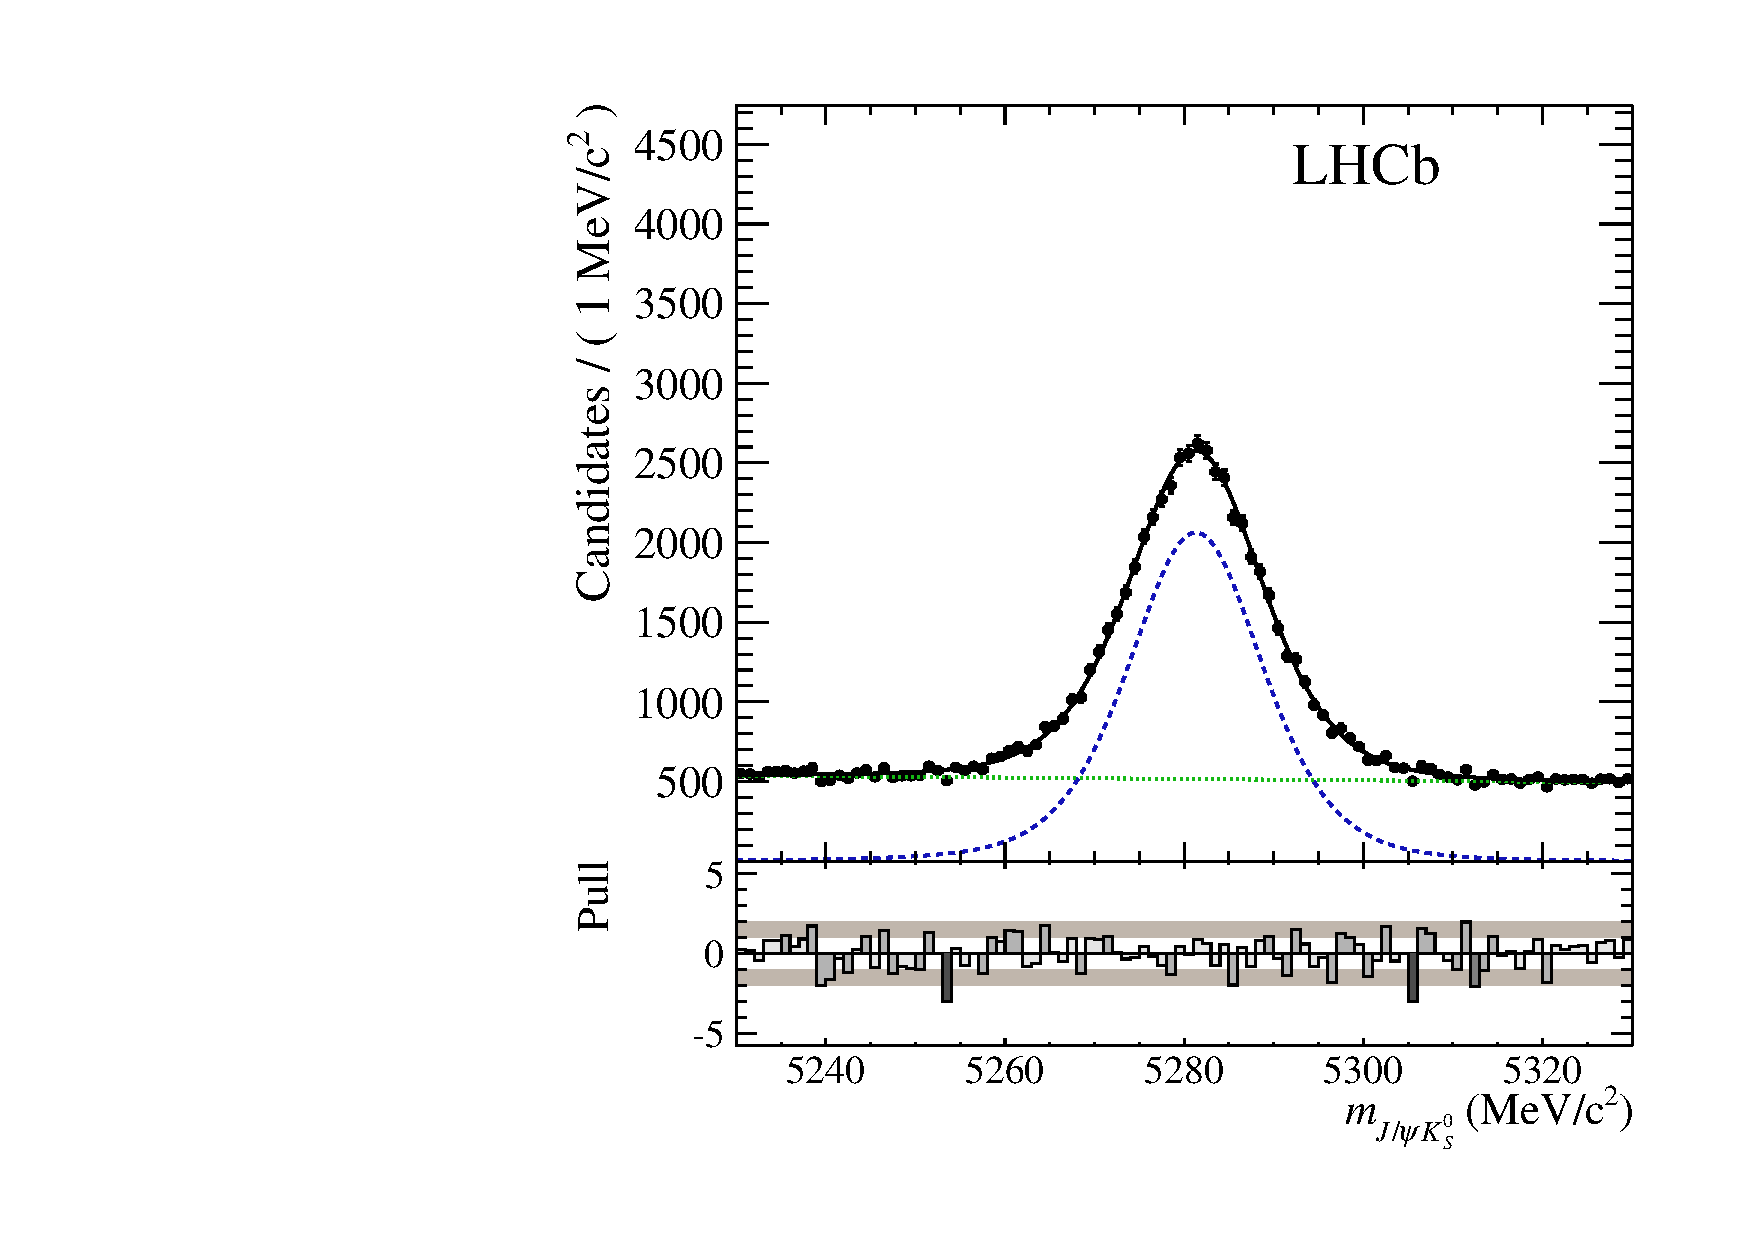
\includegraphics[width=0.4\textwidth]{private/content/measurement-of-sin2beta/figs/obsMass_summed_pull.pdf} 
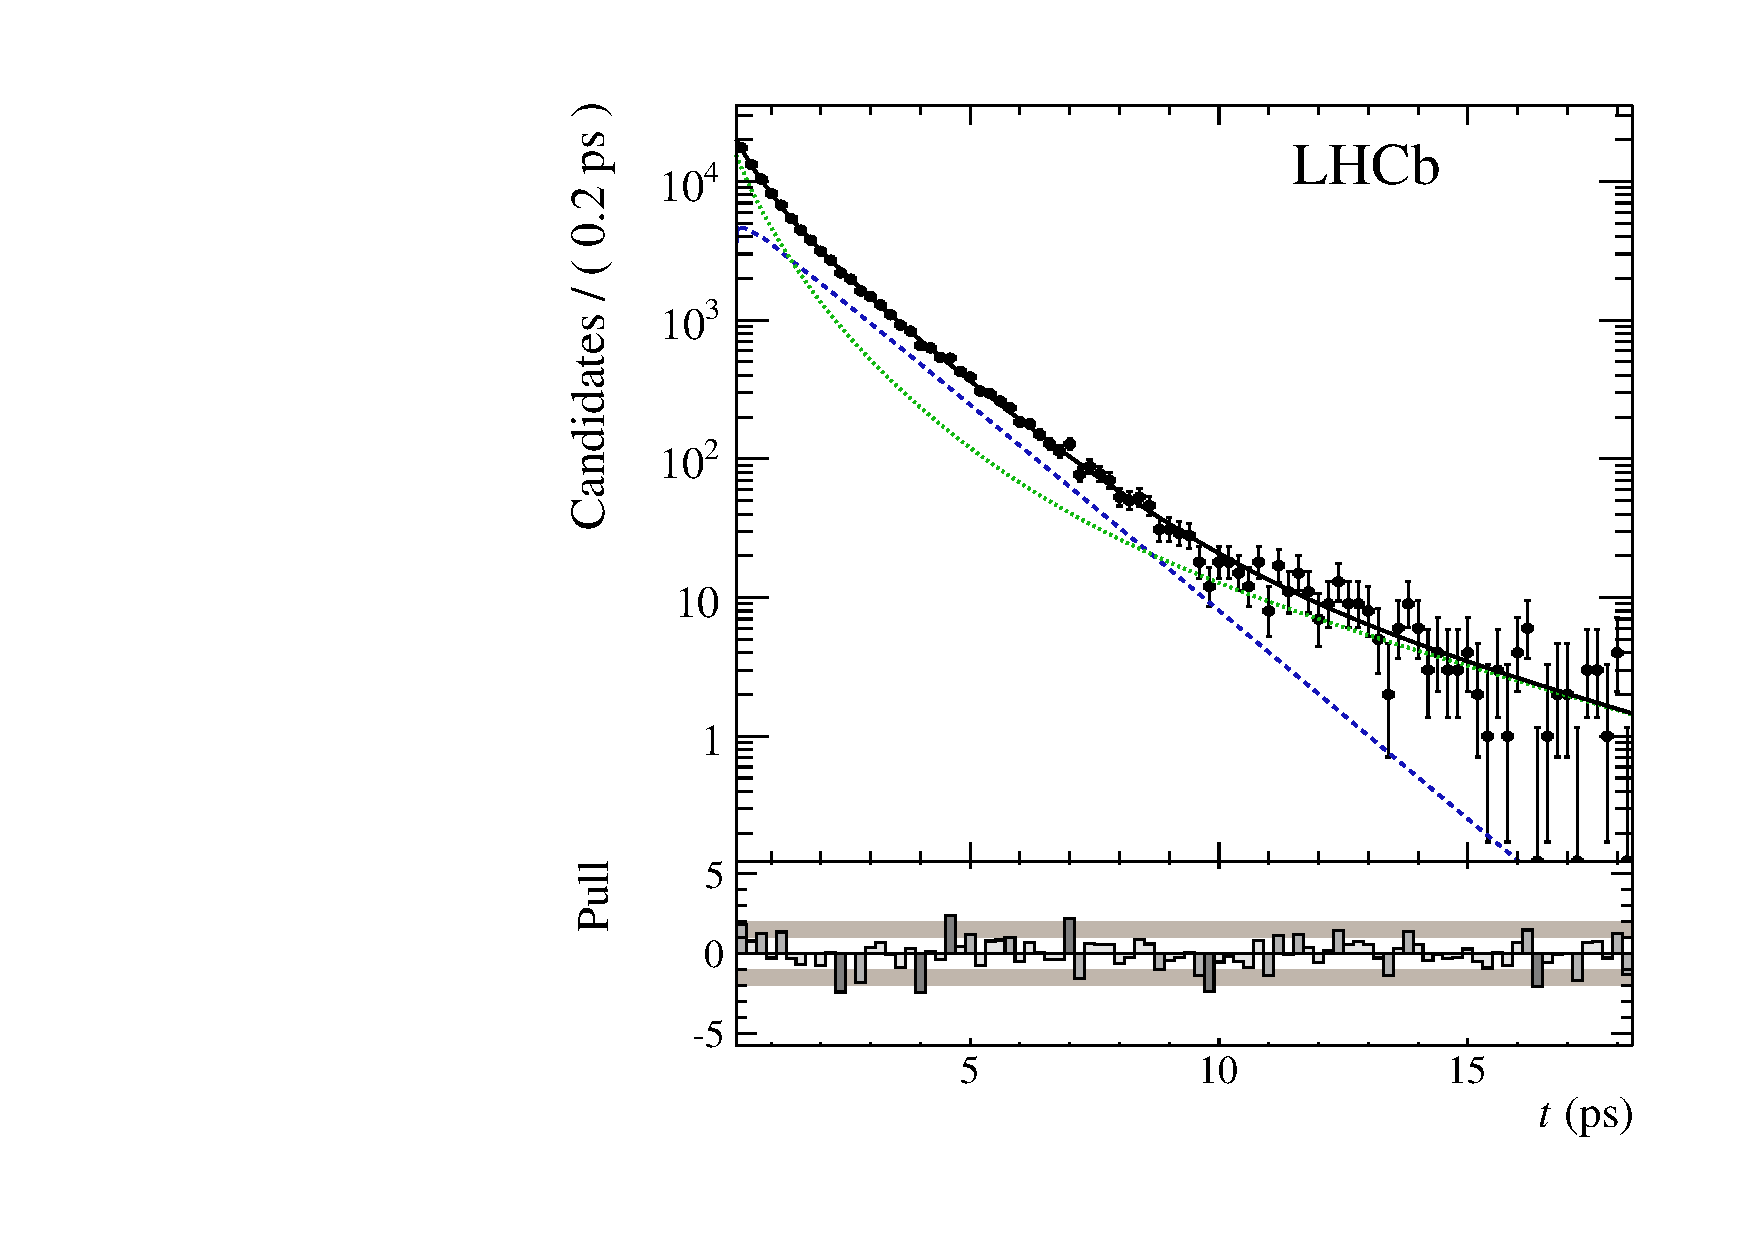
\includegraphics[width=0.4\textwidth]{private/content/measurement-of-sin2beta/figs/obsTime_summed_pull_log.pdf} \\
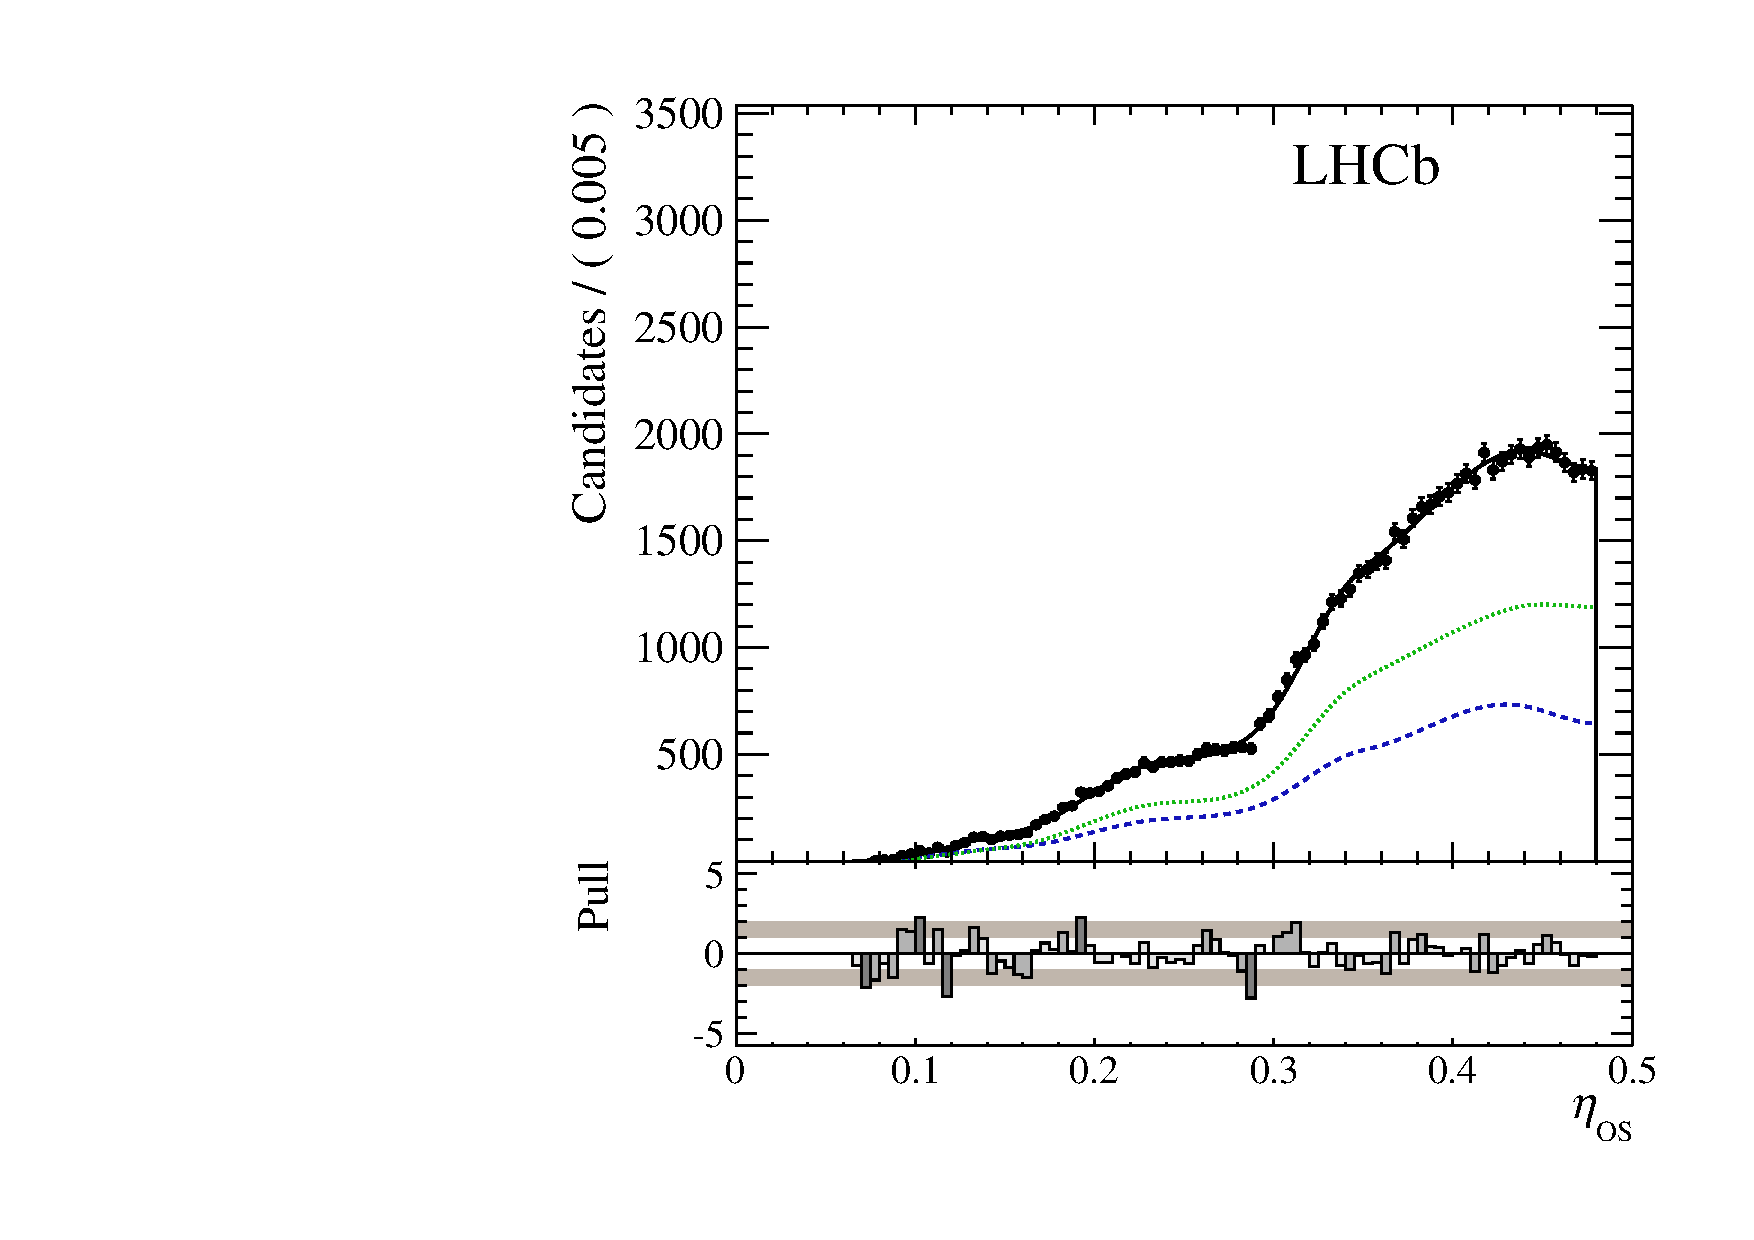
\includegraphics[width=0.4\textwidth]{private/content/measurement-of-sin2beta/figs/obsEtaOS_StdComb_CutOff_summed_pull.pdf}
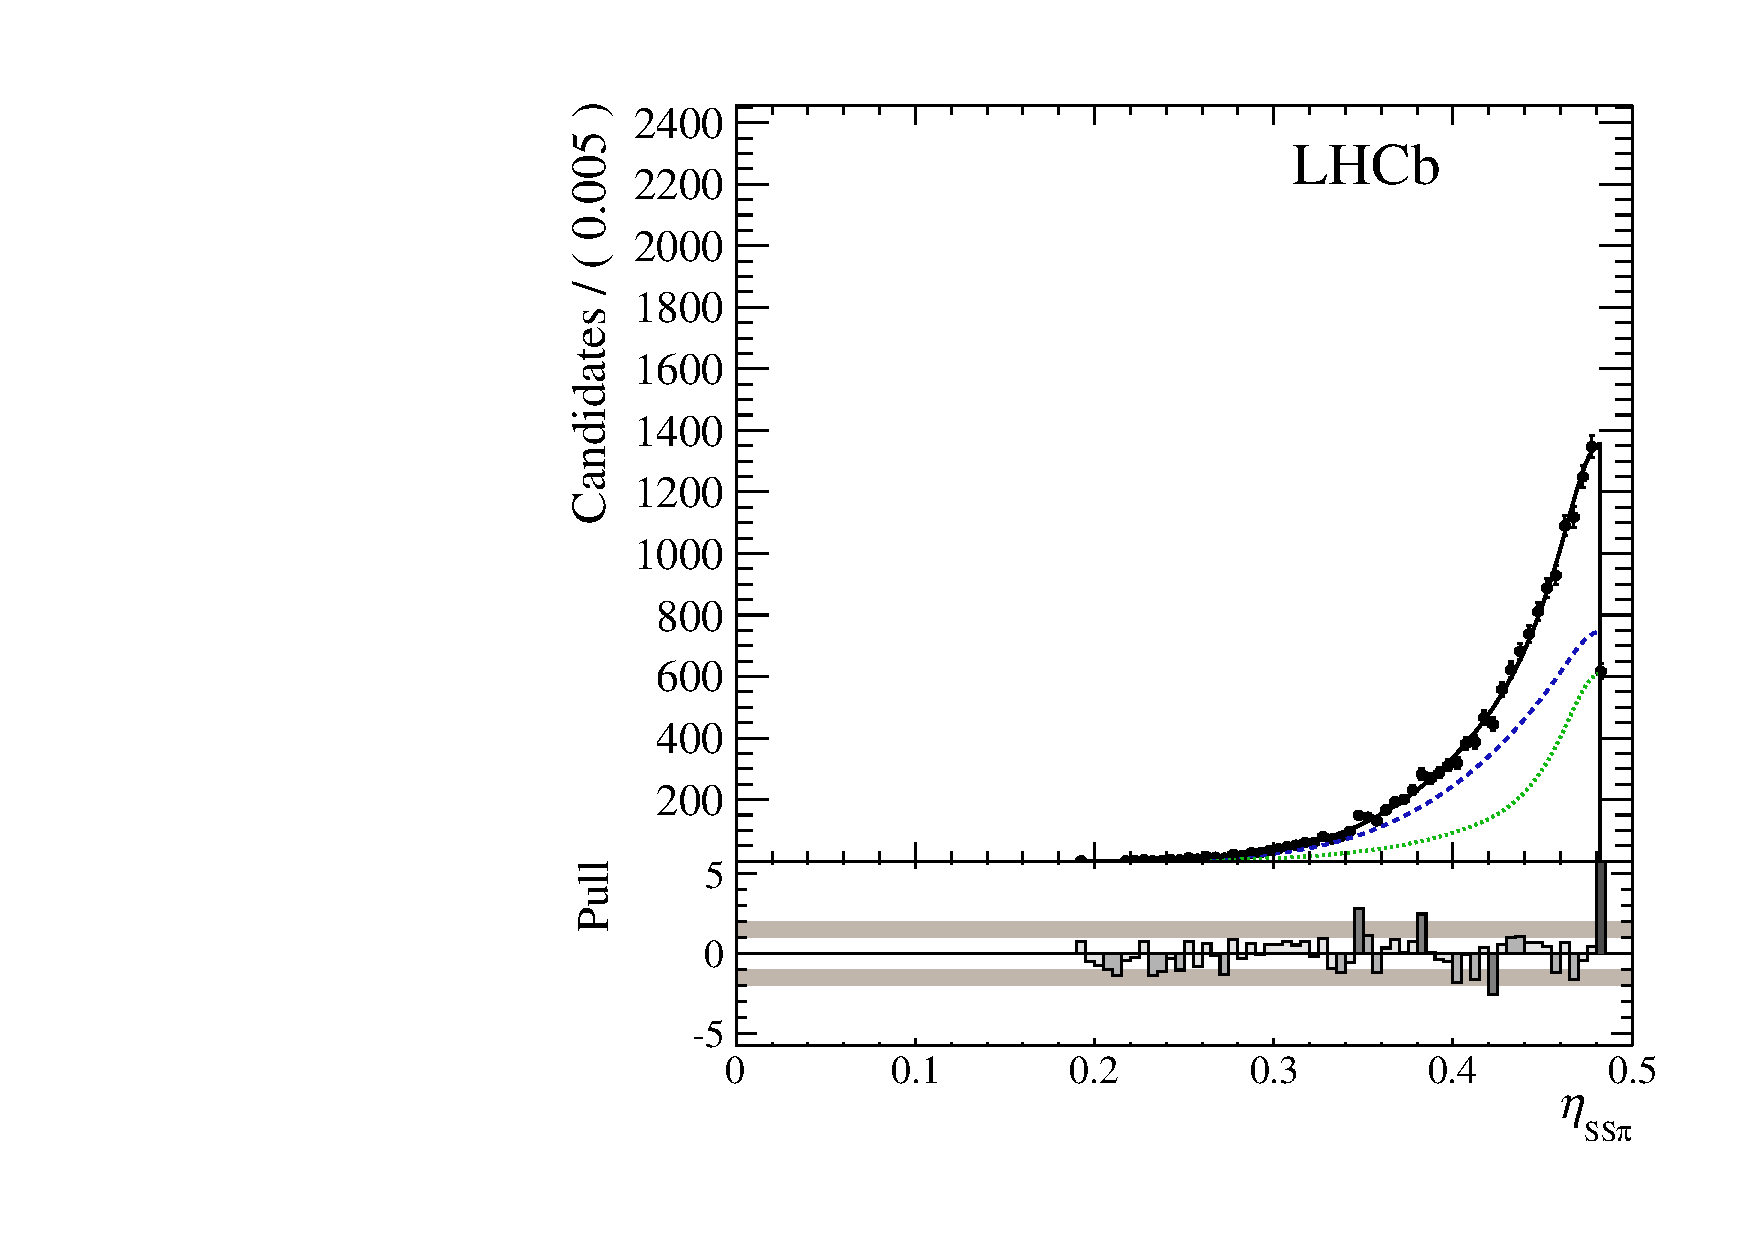
\includegraphics[width=0.4\textwidth]{private/content/measurement-of-sin2beta/figs/obsEtaSSPion_TupleCalib_summed_pull.pdf} \\
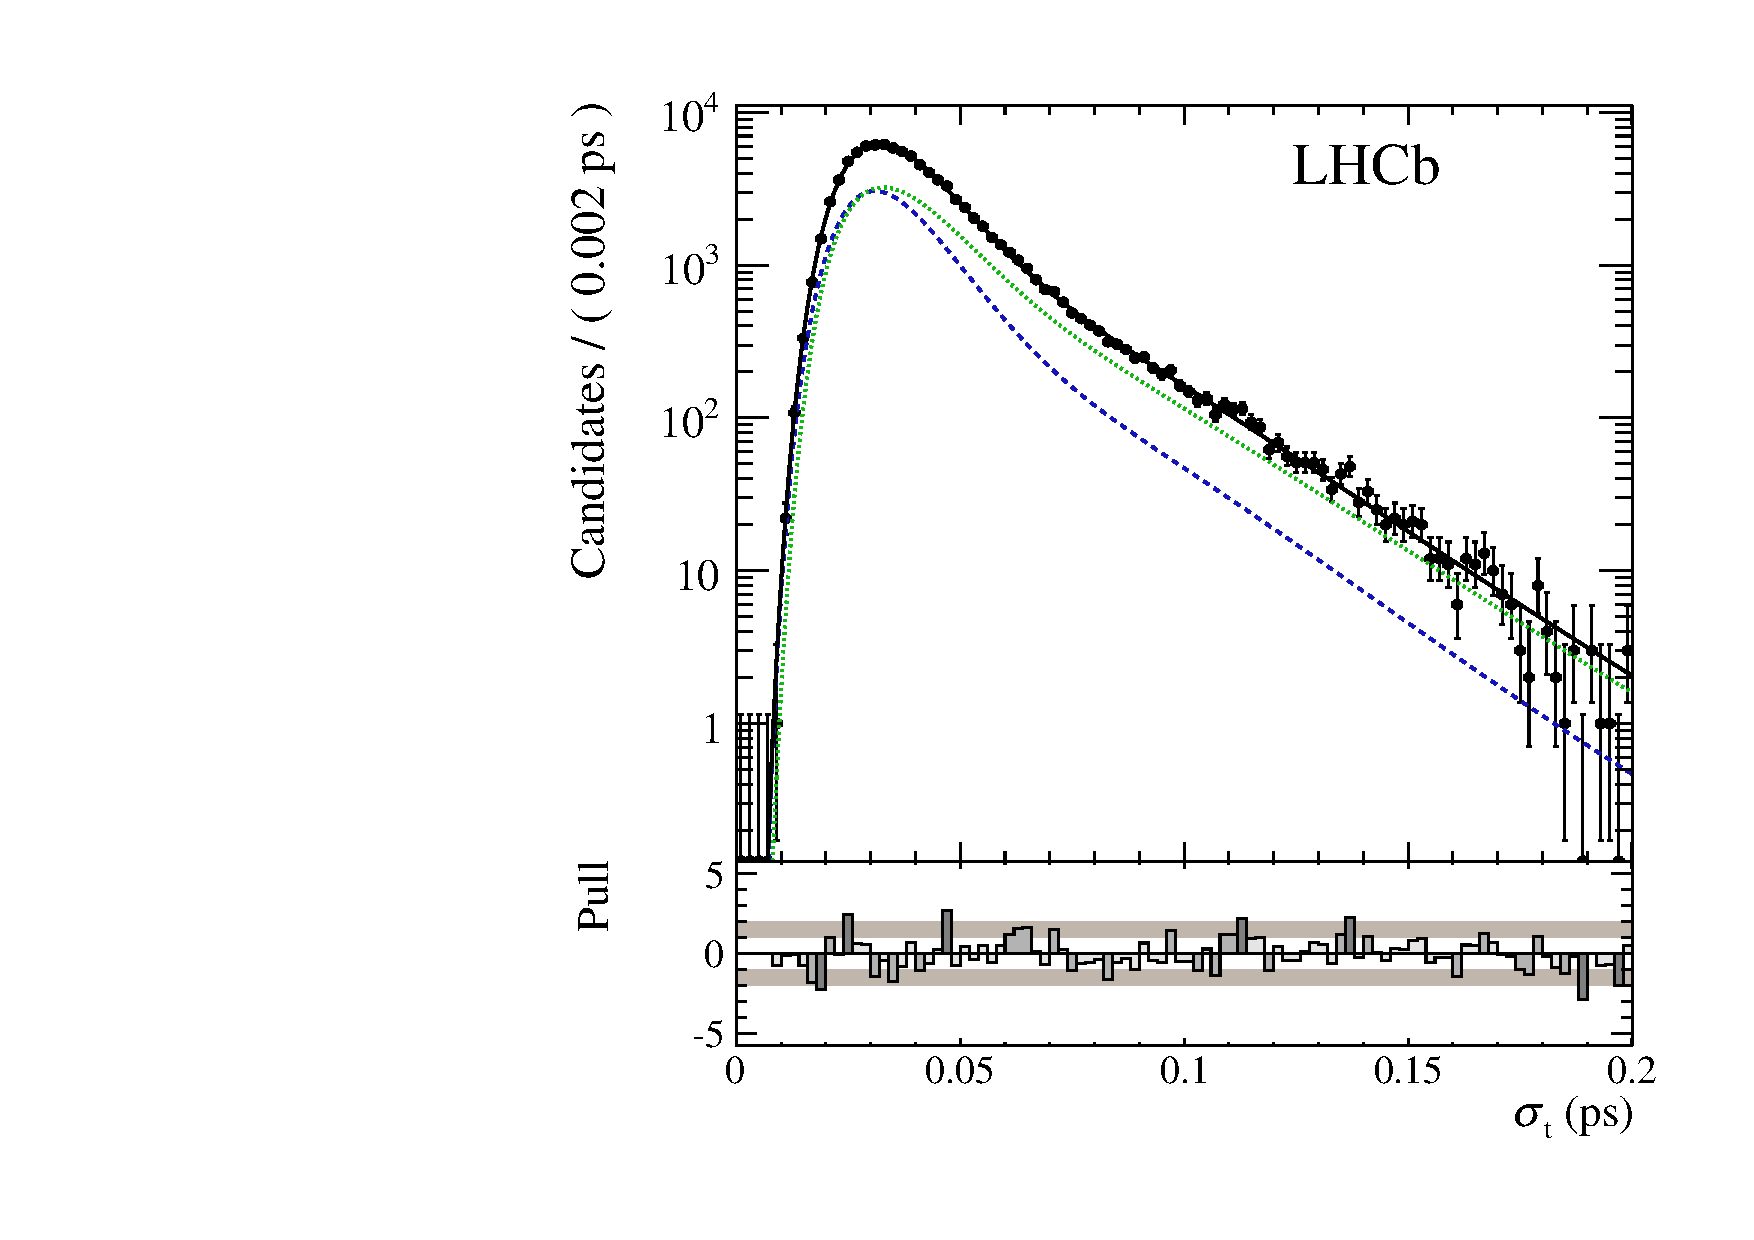
\includegraphics[width=0.4\textwidth]{private/content/measurement-of-sin2beta/figs/obsTimeError_summed_pull_log.pdf}
\caption{Plots of the \BdToJpsiKS data sample with the projected \PDF and pull
distributions. Shown is the reconstructed mass \obsMass (top left) and decay
time \obsTime (top right, logarithmic), per-event mistag (center; \obsEtaOS on
the left, \obsEtaSS on the right), and decay time error \obsTimeError (bottom,
logarithmic). Besides the data points and the full \PDF (solid black) the
projections of the signal (dashed blue) and the background (dotted green) are
shown.}
\label{fig:measurement_of_sin2beta:cpv_measurement:results:plots:dimensions}
\end{figure}

% ------------------------------------------------------------------------------
\subsection{Kaon regeneration}
\label{sec:measurement_of_sin2beta:cpv_measurement:kaon_regeneration}

\missing{Kaon regeneration}


\FloatBarrier

% %%%%%%%%%%%%%%%%%%%%%%%%%%%%%%%%%%%%%%%%%%%%%%%%%%%%%%%%%%%%%%%%%%%%%%%%%%%%%%
%!TEX root = ../../common/main.tex

\section{Studies of systematic effects}
\label{sec:measurement_of_sin2beta:systematics}

The determination of potential systematic uncertainties on the \CP parameters
complete the measurement.

The following section will describe the evaluation of systematic effects of the
fit model and influences of the flavour tagging, the decay time resolution, the
decay time acceptance, and several other inputs to the measurement of \CP
violation.

In \cref{sec:measurement_of_sin2beta:systematics:cross_checks} cross-checks are
outlined to test the reproducibility and stability of the fit model. Studies to
estimate the effect of various fit model properties are listed in
\cref{sec:measurement_of_sin2beta:systematics:systematics} while
\cref{sec:measurement_of_sin2beta:systematics:summary} gives a summary of all
found systematic effects.

% ------------------------------------------------------------------------------
\subsection{Cross-checks}
\label{sec:measurement_of_sin2beta:systematics:cross_checks}

When performing cross-checks, either results obtained on different subsamples or
results obtained from different methods on the same sample are compared. In both
cases, the deviation of the difference in fit results in terms of its
uncertainty is used as a measure of agreement.

When comparing results on different, distinct samples, the uncertainty on the
difference is estimated by summing the uncertainties of the single results in
quadrature. In contrast, when applying different methods to the same sample, the
compatibility of the results is compared by taking into account a full
correlation of the data sets. Following Ref.~\cite{Barlow:2002yb}, the
uncertainty on the difference of the two results $A$ and $B$ on the same data
set is defined as
%
\begin{equation}
  \sigma^2_\Delta = \left\vert\sigma^2_{\text{A}} - \sigma^2_{\text{B}}\right\vert .
\end{equation}
%
Again, both measurements can be interpreted as compatible if the uncertainty
lies in the same order of magnitude as the difference of the central values.

% ------------------------------------------------------------------------------
\subsubsection{Second fitter implementation}
\label{sec:measurement_of_sin2beta:systematics:cross_checks:second_fitter}
%
To provide a cross-check of the fitter implementation, two different,
independent fitter implementations were developed by the author and another
member of the working group. Being built up on the \RooFit library they do not
share any common code base. For simplification they will be denoted as
\emph{Fitter A} and \emph{Fitter B}. Both fitters are tested against each other
in the nominal fitter setup (\cref{sec:measurement_of_sin2beta:likelihood_fit}).
Applying the measure described before, the results from both fitters are in
excellent agreement, as is shown in
\Cref{fig:measurement_of_sin2beta:systematics:cross_checks:second_fitter}.
%
\begin{figure}
\centering
%!TEX root = ../main.tex

\definecolor{fcdGrayA}{HTML}{111111}
\definecolor{fcdGrayB}{HTML}{222222}
\definecolor{fcdGrayC}{HTML}{333333}
\definecolor{fcdGrayD}{HTML}{444444}
\definecolor{fcdGrayE}{HTML}{555555}
\definecolor{fcdGrayF}{HTML}{666666}
\definecolor{fcdGrayG}{HTML}{777777}
\definecolor{fcdGrayH}{HTML}{888888}
\definecolor{fcdGrayI}{HTML}{999999}
\definecolor{fcdGrayJ}{HTML}{AAAAAA}
\definecolor{fcdGrayK}{HTML}{BBBBBB}
\definecolor{fcdGrayL}{HTML}{CCCCCC}
\definecolor{fcdGrayM}{HTML}{DDDDDD}
\definecolor{fcdGrayN}{HTML}{EEEEEE}

\colorlet{ClrFitterA}{blue}
\colorlet{ClrFitterB}{red}

\begin{tikzpicture}[
  exp_label/.style={
    anchor=west,
    %minimum width=10em,
    align=left,
    font=\small\sffamily,
    inner sep=0.5em,
    outer sep=0,
  },
  exp_result/.style={
    anchor=east,
    align=right,
    font=\footnotesize\sffamily,
    inner sep=0.5em,
    outer sep=0,
    yshift=0.22em
  }
]
\begin{axis}[
  width=\textwidth,
  height=22ex,
  font=\small,
  xmin=0.62,xmax=0.80,ymin=0.3,ymax=2.7,
  xlabel={${\SJpsiKS}$},
  xlabel style={
        at={(ticklabel cs:1)},
        anchor=north east,
    },%
  xtick={0.67, 0.69, 0.71, 0.73, 0.75, 0.77},
  xticklabel style={%
    major tick length=3pt,
    /pgf/number format/fixed
  },
  hide y axis
]

\begin{pgfonlayer}{background}
  \draw[ultra thin,color=fcdGrayM,dashed]({rel axis cs:0,0}-|{axis cs:0.67,0}) -- ({rel axis cs:0.67,1}-|{axis cs:0.67,0});
  \draw[ultra thin,color=fcdGrayM,dashed]({rel axis cs:0,0}-|{axis cs:0.68,0}) -- ({rel axis cs:0.68,1}-|{axis cs:0.68,0});
  \draw[ultra thin,color=fcdGrayM,dashed]({rel axis cs:0,0}-|{axis cs:0.69,0}) -- ({rel axis cs:0.69,1}-|{axis cs:0.69,0});
  \draw[ultra thin,color=fcdGrayM,dashed]({rel axis cs:0,0}-|{axis cs:0.70,0}) -- ({rel axis cs:0.70,1}-|{axis cs:0.70,0});
  \draw[ultra thin,color=fcdGrayM,dashed]({rel axis cs:0,0}-|{axis cs:0.71,0}) -- ({rel axis cs:0.71,1}-|{axis cs:0.71,0});
  \draw[ultra thin,color=fcdGrayM,dashed]({rel axis cs:0,0}-|{axis cs:0.72,0}) -- ({rel axis cs:0.72,1}-|{axis cs:0.72,0});
  \draw[ultra thin,color=fcdGrayM,dashed]({rel axis cs:0,0}-|{axis cs:0.73,0}) -- ({rel axis cs:0.73,1}-|{axis cs:0.73,0});
  \draw[ultra thin,color=fcdGrayM,dashed]({rel axis cs:0,0}-|{axis cs:0.74,0}) -- ({rel axis cs:0.74,1}-|{axis cs:0.74,0});
  \draw[ultra thin,color=fcdGrayM,dashed]({rel axis cs:0,0}-|{axis cs:0.75,0}) -- ({rel axis cs:0.75,1}-|{axis cs:0.75,0});
  \draw[ultra thin,color=fcdGrayM,dashed]({rel axis cs:0,0}-|{axis cs:0.76,0}) -- ({rel axis cs:0.76,1}-|{axis cs:0.76,0});
  \draw[ultra thin,color=fcdGrayM,dashed]({rel axis cs:0,0}-|{axis cs:0.77,0}) -- ({rel axis cs:0.77,1}-|{axis cs:0.77,0});

  % per-event reso
  \fill[color=fcdGrayM] ({rel axis cs:0,0}-|{axis cs:0.737125640334,0}) rectangle ({rel axis cs:0.718208386766,1}-|{axis cs:0.718208386766,0});
  \fill[color=fcdGrayK] ({rel axis cs:0,0}-|{axis cs:0.732396326942,0}) rectangle ({rel axis cs:0.722937700158,1}-|{axis cs:0.722937700158,0});
  \draw[ultra thin,color=fcdGrayI]({rel axis cs:0,0}-|{axis cs:0.72766701355,0}) -- ({rel axis cs:0.72766701355,1}-|{axis cs:0.72766701355,0});
\end{pgfonlayer}

%-------------------------------------------------------------------------------
% PER_EVENT RESOLUTION
\node[exp_label, color=ClrFitterA] (FitterA_lbl) at (axis cs: \pgfkeysvalueof{/pgfplots/xmin},2)  
{Fitter A};
\node[exp_result,color=ClrFitterA] (FitterA_rsl) at (axis cs: \pgfkeysvalueof{/pgfplots/xmax},2) 
{${0.727 \pm\,^{0.034}_{0.035}}$};

\addplot+[only marks,
    thin,
    solid,
    color = ClrFitterA,
    mark=none,
    mark options={%
      scale=0.7,
      draw=ClrFitterA
    },
    error bars/.cd,
    x dir=both, x explicit,
    y dir=both, y explicit,
    error mark options={%
      rotate=90,
      mark size=5pt,
      color=ClrFitterA
    }
]
table[
        x error plus=ex+,
        x error minus=ex-,
]{
  x        y  ex+        ex-  
  0.72683  2  0.034456   0.034641
};

\node[exp_label, color=ClrFitterB] (FitterB_lbl) at (axis cs: \pgfkeysvalueof{/pgfplots/xmin},1)  
{Fitter B};
\node[exp_result,color=ClrFitterB] (FitterB_rsl) at (axis cs: \pgfkeysvalueof{/pgfplots/xmax},1) 
{${0.729 \pm 0.035}$};

\addplot+[only marks,
    thin,
    solid,
    color = ClrFitterB,
    mark=none,
    mark options={%
      scale=0.7,
      draw=ClrFitterB
    },
    error bars/.cd,
    x dir=both, x explicit,
    y dir=both, y explicit,
    error mark options={%
      rotate=90,
      mark size=5pt,
      color=ClrFitterB
    }
]
table[
        x error plus=ex+,
        x error minus=ex-,
]{
  x              y  ex+             ex-  
  0.7285040271   1  0.03461272157   0.03477905032
};

\end{axis}
\end{tikzpicture}

%!TEX root = ../main.tex

\definecolor{fcdGrayA}{HTML}{111111}
\definecolor{fcdGrayB}{HTML}{222222}
\definecolor{fcdGrayC}{HTML}{333333}
\definecolor{fcdGrayD}{HTML}{444444}
\definecolor{fcdGrayE}{HTML}{555555}
\definecolor{fcdGrayF}{HTML}{666666}
\definecolor{fcdGrayG}{HTML}{777777}
\definecolor{fcdGrayH}{HTML}{888888}
\definecolor{fcdGrayI}{HTML}{999999}
\definecolor{fcdGrayJ}{HTML}{AAAAAA}
\definecolor{fcdGrayK}{HTML}{BBBBBB}
\definecolor{fcdGrayL}{HTML}{CCCCCC}
\definecolor{fcdGrayM}{HTML}{DDDDDD}
\definecolor{fcdGrayN}{HTML}{EEEEEE}

\colorlet{ClrFitterA}{blue}
\colorlet{ClrFitterB}{red}

\begin{tikzpicture}[
  exp_label/.style={
    anchor=west,
    %minimum width=10em,
    align=left,
    font=\small\sffamily,
    inner sep=0.5em,
    outer sep=0,
  },
  exp_result/.style={
    anchor=east,
    align=right,
    font=\footnotesize\sffamily,
    inner sep=0.5em,
    outer sep=0,
    yshift=0.22em
  }
]
\begin{axis}[
  width=\textwidth,
  height=22ex,
  font=\small,
  xmin=-0.137,xmax=0.043,ymin=0.3,ymax=2.7,
  xlabel={${\CJpsiKS}$},
  xlabel style={
        at={(ticklabel cs:1)},
        anchor=north east,
    },%
  xtick={-0.09, -0.07, -0.05, -0.03, -0.01, 0.01},
  xticklabel style={%
    major tick length=3pt,
    /pgf/number format/fixed
  },
  hide y axis
]

\begin{pgfonlayer}{background}
  \draw[ultra thin,color=fcdGrayM,dashed]({rel axis cs:0,0}-|{axis cs:-0.09,0}) -- ({rel axis cs:-0.09,1}-|{axis cs:-0.09,0});
  \draw[ultra thin,color=fcdGrayM,dashed]({rel axis cs:0,0}-|{axis cs:-0.08,0}) -- ({rel axis cs:-0.08,1}-|{axis cs:-0.08,0});
  \draw[ultra thin,color=fcdGrayM,dashed]({rel axis cs:0,0}-|{axis cs:-0.07,0}) -- ({rel axis cs:-0.07,1}-|{axis cs:-0.07,0});
  \draw[ultra thin,color=fcdGrayM,dashed]({rel axis cs:0,0}-|{axis cs:-0.06,0}) -- ({rel axis cs:-0.06,1}-|{axis cs:-0.06,0});
  \draw[ultra thin,color=fcdGrayM,dashed]({rel axis cs:0,0}-|{axis cs:-0.05,0}) -- ({rel axis cs:-0.05,1}-|{axis cs:-0.05,0});
  \draw[ultra thin,color=fcdGrayM,dashed]({rel axis cs:0,0}-|{axis cs:-0.04,0}) -- ({rel axis cs:-0.04,1}-|{axis cs:-0.04,0});
  \draw[ultra thin,color=fcdGrayM,dashed]({rel axis cs:0,0}-|{axis cs:-0.03,0}) -- ({rel axis cs:-0.03,1}-|{axis cs:-0.03,0});
  \draw[ultra thin,color=fcdGrayM,dashed]({rel axis cs:0,0}-|{axis cs:-0.02,0}) -- ({rel axis cs:-0.02,1}-|{axis cs:-0.02,0});
  \draw[ultra thin,color=fcdGrayM,dashed]({rel axis cs:0,0}-|{axis cs:-0.01,0}) -- ({rel axis cs:-0.01,1}-|{axis cs:-0.01,0});
  \draw[ultra thin,color=fcdGrayM,dashed]({rel axis cs:0,0}-|{axis cs:-0.00,0}) -- ({rel axis cs:-0.00,1}-|{axis cs:-0.00,0});
  \draw[ultra thin,color=fcdGrayM,dashed]({rel axis cs:0,0}-|{axis cs:0.01,0}) -- ({rel axis cs:0.01,1}-|{axis cs:0.01,0});
  
  % per-event reso
  \fill[color=fcdGrayM] ({rel axis cs:0,0}-|{axis cs:-0.0255884399411,0}) rectangle ({rel axis cs:-0.0396240151589,1}-|{axis cs:-0.0396240151589,0});
  \fill[color=fcdGrayK] ({rel axis cs:0,0}-|{axis cs:-0.0290973337456,0}) rectangle ({rel axis cs:-0.0361151213544,1}-|{axis cs:-0.0361151213544,0});
  \draw[ultra thin,color=fcdGrayI]({rel axis cs:0,0}-|{axis cs:-0.03260622755,0}) -- ({rel axis cs:-0.03260622755,1}-|{axis cs:-0.03260622755,0});
\end{pgfonlayer}


%-------------------------------------------------------------------------------
% PER_EVENT RESOLUTION
\node[exp_label, color=ClrFitterA] (FitterA_lbl) at (axis cs: \pgfkeysvalueof{/pgfplots/xmin},2)  
{Fitter A};
\node[exp_result,color=ClrFitterA] (FitterA_rsl) at (axis cs: \pgfkeysvalueof{/pgfplots/xmax},2) 
{${-0.032 \pm 0.032}$};

\addplot+[only marks,
    thin,
    solid,
    color = ClrFitterA,
    mark=none,
    mark options={%
      scale=0.7,
      draw=ClrFitterA
    },
    error bars/.cd,
    x dir=both, x explicit,
    y dir=both, y explicit,
    error mark options={%
      rotate=90,
      mark size=5pt,
      color=ClrFitterA
    }
]
table[
        x error plus=ex+,
        x error minus=ex-,
]{
  x          y  ex+         ex-  
  -0.032078  2  0.032122   0.032312
};

\node[exp_label, color=ClrFitterB] (FitterB_lbl) at (axis cs: \pgfkeysvalueof{/pgfplots/xmin},1)  
{Fitter B};
\node[exp_result,color=ClrFitterB] (FitterB_rsl) at (axis cs: \pgfkeysvalueof{/pgfplots/xmax},1) 
{${-0.033 \pm 0.032}$};

\addplot+[only marks,
    thin,
    solid,
    color = ClrFitterB,
    mark=none,
    mark options={%
      scale=0.7,
      draw=ClrFitterB
    },
    error bars/.cd,
    x dir=both, x explicit,
    y dir=both, y explicit,
    error mark options={%
      rotate=90,
      mark size=5pt,
      color=ClrFitterB
    }
]
table[
        x error plus=ex+,
        x error minus=ex-,
]{
  x             y  ex+             ex-  
  -0.0331344551 1  0.03212091232   0.03213103531
};

\end{axis}
\end{tikzpicture}

\caption{
Fit results for \SJpsiKS and \CJpsiKS for both fitter implementations.
In blue (red) the result and the statistical error for Fitter A (B). The
grey solid line shows the average of both fit results, while the filled grey
area describes the uncertainty on the difference $\sigma_\Delta$ of the two
results (darker grey $1\sigma_\Delta$, light grey $2\sigma_\Delta$).
\textit{Please note: The shown numbers are rounded following the PDG rules. The
plot itself is produced using the full precision values.} }
\label{fig:measurement_of_sin2beta:systematics:cross_checks:second_fitter}
\end{figure}

% ------------------------------------------------------------------------------
\subsubsection{\sPlot fit}
\label{sec:measurement_of_sin2beta:systematics:cross_checks:splot_fit}
%
As the background decay time model might influence the measurement, an \sPlot fit is
performed using the nominal signal mass \PDF. As the standard \Minuit/\Hesse error
estimations in \sPlot fits can lead to uncertainties with an incorrect coverage,
an additional bootstrapping (\cf \eg \cite{Behnke:2013pga}) study is performed
to arrive at correct estimates of uncertainties. The procedure followed is:
%
\begin{enumerate}
  \item take the \sweighted data sample consisting of $N$ events,
  \item sample $N$ randomly selected events with replacement into a new data sample,
  \item perform a fit to the resulting sample to measure \SJpsiKS and \CJpsiKS,
  \item repeat the steps to obtain a distribution of the measured \CP parameters.
\end{enumerate}
%
\Cref{fig:measurement_of_sin2beta:systematics:cross_checks:splot_fit:s_and_c}
shows the fit result of the \sPlot fit with the corresponding \Hesse uncertainty
estimates, as well as the nominal fit result. Additionally, the uncertainty
estimates from the bootstrapping study are included. For the latter, the
medians of the measured \SJpsiKS and \CJpsiKS distributions are chosen as
central values, while the quoted uncertainties are the quantile-based estimates
for two-sided $\SI{68.27}{\percent}$ quantiles of the same distribution. The
resulting distributions based on $\num{1000}$ bootstrapping iterations are
presented in
\cref{fig:measurement_of_sin2beta:systematics:cross_checks:splot_fit:bootstrapping}.

The central values resulting from the bootstrapped \sPlot fits are very well
compatible with the naive \sPlot fit. Compared to the nominal fit this holds
true for \CJpsiKS while \SJpsiKS is slightly lower. The uncertainty estimates of
the bootstrapping study are slightly larger than the corresponding uncertainties
from the nominal fit, but still in the same order of magnitude. In contrast, the
uncertainty estimate of the naive \sPlot fit for \SJpsiKS, should be larger or
at the best equal of size compared to the nominal fit, but are found to be too
small. Overall, the results of the \sPlot fits and the nominal fit are well
compatible.
%
\begin{figure}
\centering
%!TEX root = ../main.tex

\definecolor{fcdGrayA}{HTML}{111111}
\definecolor{fcdGrayB}{HTML}{222222}
\definecolor{fcdGrayC}{HTML}{333333}
\definecolor{fcdGrayD}{HTML}{444444}
\definecolor{fcdGrayE}{HTML}{555555}
\definecolor{fcdGrayF}{HTML}{666666}
\definecolor{fcdGrayG}{HTML}{777777}
\definecolor{fcdGrayH}{HTML}{888888}
\definecolor{fcdGrayI}{HTML}{999999}
\definecolor{fcdGrayJ}{HTML}{AAAAAA}
\definecolor{fcdGrayK}{HTML}{BBBBBB}
\definecolor{fcdGrayL}{HTML}{CCCCCC}
\definecolor{fcdGrayM}{HTML}{DDDDDD}
\definecolor{fcdGrayN}{HTML}{EEEEEE}

\colorlet{ClrSFit}{blue}
\colorlet{ClrSFitBT}{blue}
\colorlet{ClrNominalFit}{red}

\begin{tikzpicture}[
  exp_label/.style={
    anchor=west,
    %minimum width=10em,
    align=left,
    font=\small\sffamily,
    inner sep=0.5em,
    outer sep=0,
  },
  exp_result/.style={
    anchor=east,
    align=right,
    font=\footnotesize\sffamily,
    inner sep=0.5em,
    outer sep=0,
    yshift=0.22em
  }
]
\begin{axis}[
  width=\textwidth,
  height=30ex,
  font=\small,
  xmin=0.62,xmax=0.80,ymin=0.3,ymax=3.7,
  xlabel={${\SJpsiKS}$},
  xlabel style={
        at={(ticklabel cs:1)},
        anchor=north east,
    },%
  xtick={0.67, 0.69, 0.71, 0.73, 0.75, 0.77},
  xticklabel style={%
    major tick length=3pt,
    /pgf/number format/fixed
  },
  hide y axis
]

\begin{pgfonlayer}{background}
  \draw[ultra thin,color=fcdGrayM,dashed]({rel axis cs:0,0}-|{axis cs:0.67,0}) -- ({rel axis cs:0.67,1}-|{axis cs:0.67,0});
  \draw[ultra thin,color=fcdGrayM,dashed]({rel axis cs:0,0}-|{axis cs:0.68,0}) -- ({rel axis cs:0.68,1}-|{axis cs:0.68,0});
  \draw[ultra thin,color=fcdGrayM,dashed]({rel axis cs:0,0}-|{axis cs:0.69,0}) -- ({rel axis cs:0.69,1}-|{axis cs:0.69,0});
  \draw[ultra thin,color=fcdGrayM,dashed]({rel axis cs:0,0}-|{axis cs:0.70,0}) -- ({rel axis cs:0.70,1}-|{axis cs:0.70,0});
  \draw[ultra thin,color=fcdGrayM,dashed]({rel axis cs:0,0}-|{axis cs:0.71,0}) -- ({rel axis cs:0.71,1}-|{axis cs:0.71,0});
  \draw[ultra thin,color=fcdGrayM,dashed]({rel axis cs:0,0}-|{axis cs:0.72,0}) -- ({rel axis cs:0.72,1}-|{axis cs:0.72,0});
  \draw[ultra thin,color=fcdGrayM,dashed]({rel axis cs:0,0}-|{axis cs:0.73,0}) -- ({rel axis cs:0.73,1}-|{axis cs:0.73,0});
  \draw[ultra thin,color=fcdGrayM,dashed]({rel axis cs:0,0}-|{axis cs:0.74,0}) -- ({rel axis cs:0.74,1}-|{axis cs:0.74,0});
  \draw[ultra thin,color=fcdGrayM,dashed]({rel axis cs:0,0}-|{axis cs:0.75,0}) -- ({rel axis cs:0.75,1}-|{axis cs:0.75,0});
  \draw[ultra thin,color=fcdGrayM,dashed]({rel axis cs:0,0}-|{axis cs:0.76,0}) -- ({rel axis cs:0.76,1}-|{axis cs:0.76,0});
  \draw[ultra thin,color=fcdGrayM,dashed]({rel axis cs:0,0}-|{axis cs:0.77,0}) -- ({rel axis cs:0.77,1}-|{axis cs:0.77,0});

  % 2 sigma error band
  \fill[color=fcdGrayM] ({rel axis cs:0,0}-|{axis cs:0.72510503111,0}) rectangle ({rel axis cs:0.71465031339,1}-|{axis cs:0.71465031339,0});
  % 1 sigma error band
  \fill[color=fcdGrayK] ({rel axis cs:0,0}-|{axis cs:0.72249135168,0}) rectangle ({rel axis cs:0.71726399282,1}-|{axis cs:0.71726399282,0});
  % average
  \draw[ultra thin,color=fcdGrayI]({rel axis cs:0,0}-|{axis cs:0.71987767225,0}) -- ({rel axis cs:0.71987767225,1}-|{axis cs:0.71987767225,0});
\end{pgfonlayer}

\node[exp_label, color=ClrSFit] (SFit_lbl) at (axis cs: \pgfkeysvalueof{/pgfplots/xmin},3)  
{\sPlot fit\\[-0.3ex]\footnotesize \Hesse};
\node[exp_result,color=ClrSFit] (SFit_rsl) at (axis cs: \pgfkeysvalueof{/pgfplots/xmax},3) 
{${0.710 \pm 0.027}$};

\addplot+[only marks,
    thin,
    solid,
    color = ClrSFit,
    mark=none,
    mark options={%
      scale=0.7,
      draw=ClrSFit
    },
    error bars/.cd,
    x dir=both, x explicit,
    y dir=both, y explicit,
    error mark options={%
      rotate=90,
      mark size=5pt,
      color=ClrSFit
    }
]
table[
        x error plus=ex+,
        x error minus=ex-,
]{
  x            y  ex+            ex-  
  0.7103944525 3  0.02727126003  0.02727126003
};

\node[exp_label, color=ClrSFitBT] (SFit_lbl) at (axis cs: \pgfkeysvalueof{/pgfplots/xmin},2)  
{\sPlot\\[-0.3ex]\footnotesize bootstrapped fits};
\node[exp_result,color=ClrSFitBT] (SFit_rsl) at (axis cs: \pgfkeysvalueof{/pgfplots/xmax},2) 
{${0.711 \pm\,^{0.035}_{0.036}}$};

\addplot+[only marks,
    thin,
    solid,
    color = ClrSFitBT,
    mark=none,
    mark options={%
      scale=0.7,
      draw=ClrSFitBT
    },
    error bars/.cd,
    x dir=both, x explicit,
    y dir=both, y explicit,
    error mark options={%
      rotate=90,
      mark size=5pt,
      color=ClrSFitBT
    }
]
table[
        x error plus=ex+,
        x error minus=ex-,
]{
  x            y  ex+           ex-  
  0.7112513174 2  0.03487712232 0.03601769196
};

\node[exp_label, color=ClrNominalFit] (NominalFit_lbl) at (axis cs: \pgfkeysvalueof{/pgfplots/xmin},1)  
{Nominal fit};
\node[exp_result,color=ClrNominalFit] (NominalFit_rsl) at (axis cs: \pgfkeysvalueof{/pgfplots/xmax},1) 
{${0.729 \pm 0.035}$};

\addplot+[only marks,
    thin,
    solid,
    color = ClrNominalFit,
    mark=none,
    mark options={%
      scale=0.7,
      draw=ClrNominalFit
    },
    error bars/.cd,
    x dir=both, x explicit,
    y dir=both, y explicit,
    error mark options={%
      rotate=90,
      mark size=5pt,
      color=ClrNominalFit
    }
]
table[
        x error plus=ex+,
        x error minus=ex-,
]{
  x            y  ex+             ex-  
  0.7285040271 1 0.03461272157    0.03477905032
};

\end{axis}
\end{tikzpicture}

%!TEX root = ../main.tex

\definecolor{fcdGrayA}{HTML}{111111}
\definecolor{fcdGrayB}{HTML}{222222}
\definecolor{fcdGrayC}{HTML}{333333}
\definecolor{fcdGrayD}{HTML}{444444}
\definecolor{fcdGrayE}{HTML}{555555}
\definecolor{fcdGrayF}{HTML}{666666}
\definecolor{fcdGrayG}{HTML}{777777}
\definecolor{fcdGrayH}{HTML}{888888}
\definecolor{fcdGrayI}{HTML}{999999}
\definecolor{fcdGrayJ}{HTML}{AAAAAA}
\definecolor{fcdGrayK}{HTML}{BBBBBB}
\definecolor{fcdGrayL}{HTML}{CCCCCC}
\definecolor{fcdGrayM}{HTML}{DDDDDD}
\definecolor{fcdGrayN}{HTML}{EEEEEE}

\colorlet{ClrSFit}{blue}
\colorlet{ClrSFitBT}{blue}
\colorlet{ClrNominalFit}{red}

\begin{tikzpicture}[
  exp_label/.style={
    anchor=west,
    %minimum width=10em,
    align=left,
    font=\small\sffamily,
    inner sep=0.5em,
    outer sep=0,
  },
  exp_result/.style={
    anchor=east,
    align=right,
    font=\footnotesize\sffamily,
    inner sep=0.5em,
    outer sep=0,
    yshift=0.22em
  }
]
\begin{axis}[
  width=\textwidth,
  height=30ex,
  font=\small,
  xmin=-0.117,xmax=0.063,ymin=0.3,ymax=3.7,
  xlabel={${\CJpsiKS}$},
  xlabel style={
        at={(ticklabel cs:1)},
        anchor=north east,
    },%
  xtick={-0.07, -0.05, -0.03, -0.01, 0.01, 0.03},
  xticklabel style={%
    major tick length=3pt,
    /pgf/number format/fixed
  },
  hide y axis
]

\begin{pgfonlayer}{background}
  \draw[ultra thin,color=fcdGrayM,dashed]({rel axis cs:0,0}-|{axis cs:-0.07,0}) -- ({rel axis cs:-0.07,1}-|{axis cs:-0.07,0});
  \draw[ultra thin,color=fcdGrayM,dashed]({rel axis cs:0,0}-|{axis cs:-0.06,0}) -- ({rel axis cs:-0.06,1}-|{axis cs:-0.06,0});
  \draw[ultra thin,color=fcdGrayM,dashed]({rel axis cs:0,0}-|{axis cs:-0.05,0}) -- ({rel axis cs:-0.05,1}-|{axis cs:-0.05,0});
  \draw[ultra thin,color=fcdGrayM,dashed]({rel axis cs:0,0}-|{axis cs:-0.04,0}) -- ({rel axis cs:-0.04,1}-|{axis cs:-0.04,0});
  \draw[ultra thin,color=fcdGrayM,dashed]({rel axis cs:0,0}-|{axis cs:-0.03,0}) -- ({rel axis cs:-0.03,1}-|{axis cs:-0.03,0});
  \draw[ultra thin,color=fcdGrayM,dashed]({rel axis cs:0,0}-|{axis cs:-0.02,0}) -- ({rel axis cs:-0.02,1}-|{axis cs:-0.02,0});
  \draw[ultra thin,color=fcdGrayM,dashed]({rel axis cs:0,0}-|{axis cs:-0.01,0}) -- ({rel axis cs:-0.01,1}-|{axis cs:-0.01,0});
  \draw[ultra thin,color=fcdGrayM,dashed]({rel axis cs:0,0}-|{axis cs:-0.00,0}) -- ({rel axis cs:-0.00,1}-|{axis cs:-0.00,0});
  \draw[ultra thin,color=fcdGrayM,dashed]({rel axis cs:0,0}-|{axis cs: 0.01,0}) -- ({rel axis cs: 0.01,1}-|{axis cs: 0.01,0});
  \draw[ultra thin,color=fcdGrayM,dashed]({rel axis cs:0,0}-|{axis cs: 0.02,0}) -- ({rel axis cs: 0.02,1}-|{axis cs: 0.02,0});
  \draw[ultra thin,color=fcdGrayM,dashed]({rel axis cs:0,0}-|{axis cs: 0.03,0}) -- ({rel axis cs: 0.03,1}-|{axis cs: 0.03,0});

  % 2 sigma error band
  \fill[color=fcdGrayM] ({rel axis cs:0,0}-|{axis cs:-0.00103402373304,0}) rectangle ({rel axis cs:-0.042529957587,1}-|{axis cs:-0.042529957587,0});
  % 1 sigma error band
  \fill[color=fcdGrayK] ({rel axis cs:0,0}-|{axis cs:-0.0114080071965,0}) rectangle ({rel axis cs:-0.0321559741235,1}-|{axis cs:-0.0321559741235,0});
  % average
  \draw[ultra thin,color=fcdGrayI]({rel axis cs:0,0}-|{axis cs:-0.02178199066,0}) -- ({rel axis cs:-0.02178199066,1}-|{axis cs:-0.02178199066,0});
\end{pgfonlayer}

\node[exp_label, color=ClrSFit] (SFit_lbl) at (axis cs: \pgfkeysvalueof{/pgfplots/xmin},3)  
{\sPlot fit\\[-0.3ex]\footnotesize \Hesse};
\node[exp_result,color=ClrSFit] (SFit_rsl) at (axis cs: \pgfkeysvalueof{/pgfplots/xmax},3) 
{${-0.011 \pm 0.037}$};

\addplot+[only marks,
    thin,
    solid,
    color = ClrSFit,
    mark=none,
    mark options={%
      scale=0.7,
      draw=ClrSFit
    },
    error bars/.cd,
    x dir=both, x explicit,
    y dir=both, y explicit,
    error mark options={%
      rotate=90,
      mark size=5pt,
      color=ClrSFit
    }
]
table[
        x error plus=ex+,
        x error minus=ex-,
]{
  x              y  ex+             ex-  
  -0.01110790192 3  0.03708065836   0.03708065836
};

\node[exp_label, color=ClrSFitBT] (SFit_lbl) at (axis cs: \pgfkeysvalueof{/pgfplots/xmin},2)  
{\sPlot\\[-0.3ex]\footnotesize bootstrapped fits};
\node[exp_result,color=ClrSFitBT] (SFit_rsl) at (axis cs: \pgfkeysvalueof{/pgfplots/xmax},2) 
{${-0.010 \pm\,^{0.038}_{0.034}}$};

\addplot+[only marks,
    thin,
    solid,
    color = ClrSFitBT,
    mark=none,
    mark options={%
      scale=0.7,
      draw=ClrSFitBT
    },
    error bars/.cd,
    x dir=both, x explicit,
    y dir=both, y explicit,
    error mark options={%
      rotate=90,
      mark size=5pt,
      color=ClrSFitBT
    }
]
table[
        x error plus=ex+,
        x error minus=ex-,
]{
  x              y  ex+             ex-  
  -0.01042952622 2  0.03750748602   0.03375459289
};

\node[exp_label, color=ClrNominalFit] (NominalFit_lbl) at (axis cs: \pgfkeysvalueof{/pgfplots/xmin},1)  
{Nominal fit};
\node[exp_result,color=ClrNominalFit] (NominalFit_rsl) at (axis cs: \pgfkeysvalueof{/pgfplots/xmax},1) 
{${-0.033 \pm 0.032}$};

\addplot+[only marks,
    thin,
    solid,
    color = ClrNominalFit,
    mark=none,
    mark options={%
      scale=0.7,
      draw=ClrNominalFit
    },
    error bars/.cd,
    x dir=both, x explicit,
    y dir=both, y explicit,
    error mark options={%
      rotate=90,
      mark size=5pt,
      color=ClrNominalFit
    }
]
table[
        x error plus=ex+,
        x error minus=ex-,
]{
  x             y  ex+             ex-  
  -0.0331344551 1  0.03212091232   0.03213103531
};

\end{axis}
\end{tikzpicture}

\caption{
Fit results for \SJpsiKS and \CJpsiKS from the \sPlot fit and the nominal fit as
a reference. In blue (red) the result and the statistical error for the \sPlot
fit (nominal fit)s. The grey solid line shows the average of the two below fit
results, while the filled grey area describes the uncertainty on the difference
$\sigma_\Delta$ of the two lower results (darker grey $1\sigma_\Delta$, light
grey $2\sigma_\Delta$).
\textit{Please note: The shown numbers are rounded following the PDG rules. The
plot itself is produced using the full precision values.}}
\label{fig:measurement_of_sin2beta:systematics:cross_checks:splot_fit:s_and_c}
\end{figure}
%
\begin{figure}
\centering
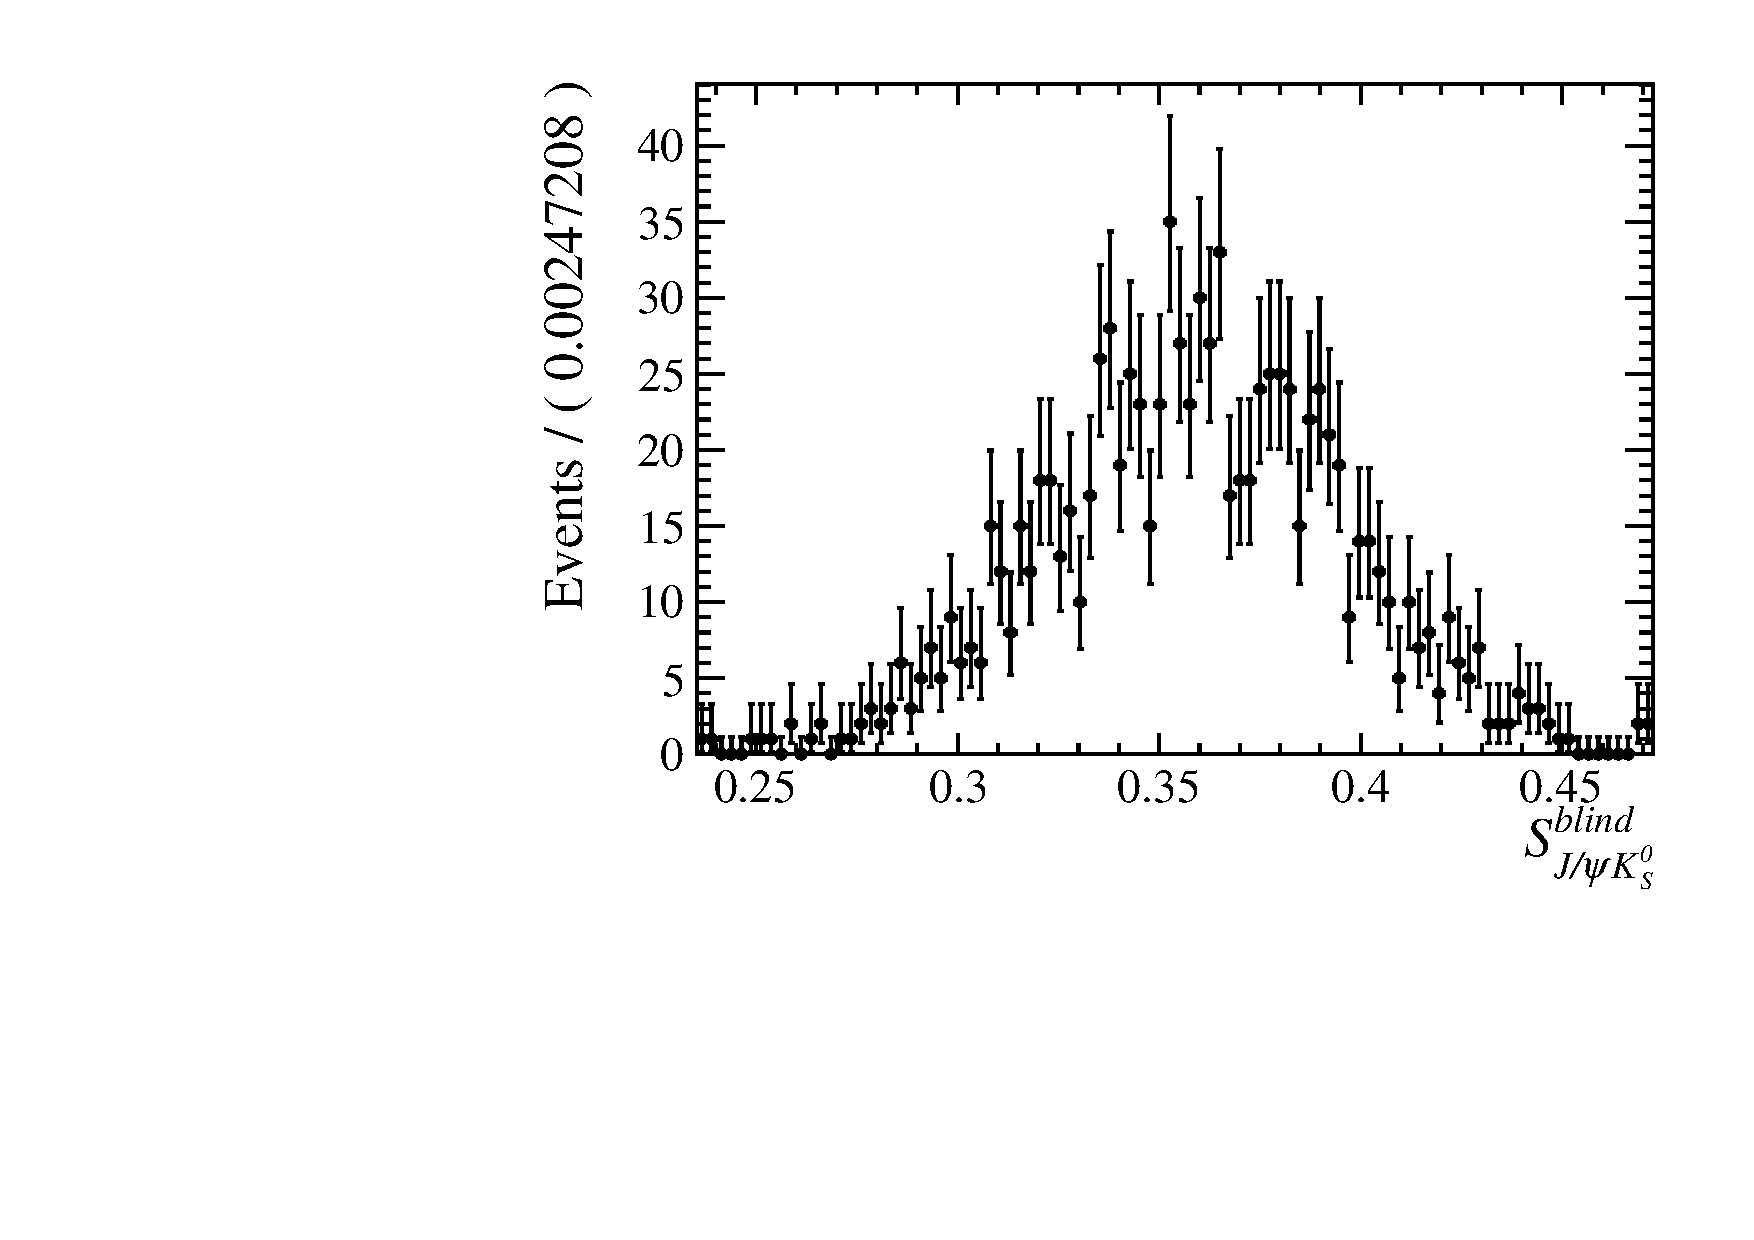
\includegraphics[width=0.48\textwidth]{private/content/measurement-of-sin2beta/figs/bootstrapping_parSigTimeSin2b_blind.pdf}
\hfill
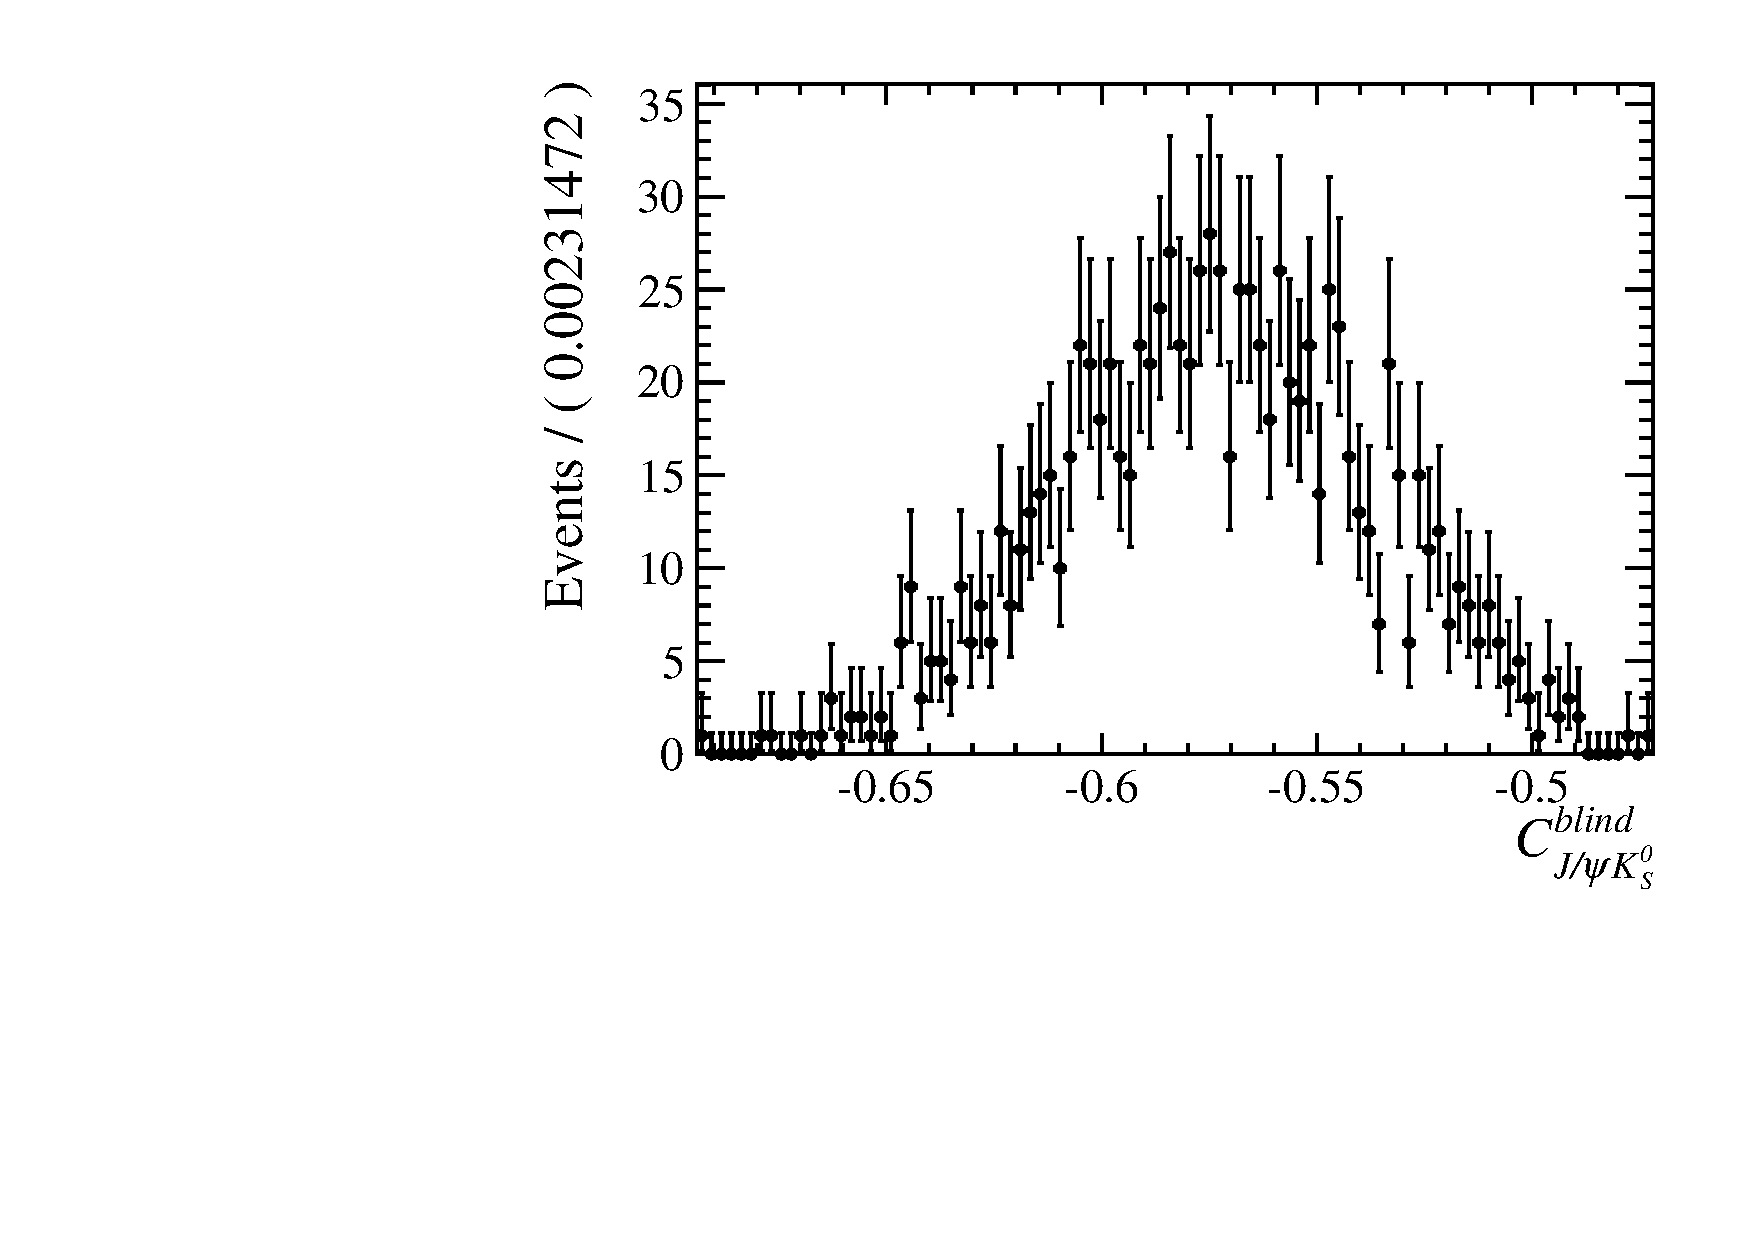
\includegraphics[width=0.48\textwidth]{private/content/measurement-of-sin2beta/figs/bootstrapping_parSigTimeCjpsiKS_blind.pdf}
\caption{
Parameter distributions for $\SJpsiKS^{\text{blind}}$ and
$\CJpsiKS^{\text{blind}}$ from \sPlot fits to $\num{1000}$ bootstrapped data
samples. The study was performed with still blinded parameter values (\cf
\cref{sec:measurement_of_sin2beta:likelihood_fit:blinding}).}
\label{fig:measurement_of_sin2beta:systematics:cross_checks:splot_fit:bootstrapping}
\end{figure}

% ------------------------------------------------------------------------------
\subsubsection{Subsamples}
\label{sec:measurement_of_sin2beta:systematics:cross_checks:subsamples}
%
To check for possible systematic effects, fits in different subsamples of the
nominal data set are conducted. The cross-checks are performed in categories of
track type (\catDD \vs \catLL), trigger requirement (\catAU \vs \catEB), tagging
algorithm (\catOS \vs \catSS \vs \catBS), magnet polarity (Up \vs Down), and
admixtures of those together with the year of data-taking (\catOO \vs \catOT).
As a control sample the full data set is also split randomly into five disjoint
subsets (Rndm1-5). \Cref{fig:measurement_of_sin2beta:systematics:cross_checks:subsamples:s_and_c}
illustrates the outcome. No significant deviation is present.
%
\begin{figure}
\centering
%!TEX root = ../main.tex

\definecolor{Black}{HTML}{000000}
\definecolor{Red}{HTML}{FC5716}

\colorlet{ClrRndm}{Black}
\colorlet{ClrTrigger}{Black}
\colorlet{ClrTagger}{Black}
\colorlet{ClrYear}{Black}
\colorlet{ClrYearTagger}{Black}
\colorlet{ClrTrack}{Black}
\colorlet{ClrFullFit}{Red}
\colorlet{ClrUncert}{Red!40}

\begin{tikzpicture}[
  exp_label/.style={
    anchor=west,
    %minimum width=10em,
    align=left,
    font=\small\sffamily,
    inner sep=0.5em,
    outer sep=0,
  },
  exp_result/.style={
    anchor=east,
    align=right,
    font=\footnotesize\sffamily,
    inner sep=0.5em,
    outer sep=0,
    yshift=0.22em
  }
]
\begin{axis}[
  width=\textwidth,
  height=65ex,
  font=\small,
  xmin=0.1,xmax=1.1,ymin=0.3,ymax=23.7,
  xlabel={$\SJpsiKS$},
  xlabel style={
        at={(ticklabel cs:1)},
        anchor=north east,
    },%
  xtick={0.3, 0.4, 0.5, 0.6, 0.7, 0.8, 0.9, 1.0},
  % xticklabels={,,},
  xticklabel style={%
    major tick length=3pt
  },
  hide y axis
]

\begin{pgfonlayer}{background}
% line at 0
% \draw[ultra thin,color=Black!80]({rel axis cs:0,0}-|{axis cs:0,0}) -- ({rel axis cs:0,1}-|{axis cs:0,0});
% line at -1
% \draw[ultra thin,color=Black!80,dashed]({rel axis cs:0,0}-|{axis cs:-1,0}) -- ({rel axis cs:-1,1}-|{axis cs:-1,0});
% line at +1
% \draw[ultra thin,color=Black!80,dashed]({rel axis cs:0,0}-|{axis cs:+1,0}) -- ({rel axis cs:+1,1}-|{axis cs:+1,0});
% filled area at average value
\fill[color=ClrUncert] ({rel axis cs:0,0}-|{axis cs:0.693724977,0}) rectangle ({rel axis cs:0.763116749,1}-|{axis cs:0.763116749,0});
% line at average value
\draw[ultra thin,color=ClrFullFit]({rel axis cs:0,0}-|{axis cs:0.7285040271,0}) -- ({rel axis cs:0.7285040271,1}-|{axis cs:0.7285040271,0});

% lines to separate the different subsamples categories
\draw[ultra thin, dashed, color=Black!80] (axis cs: \pgfkeysvalueof{/pgfplots/xmin},18.5) -- (axis cs: \pgfkeysvalueof{/pgfplots/xmax},18.5);
\draw[ultra thin, dashed, color=Black!80] (axis cs: \pgfkeysvalueof{/pgfplots/xmin},16.5) -- (axis cs: \pgfkeysvalueof{/pgfplots/xmax},16.5);
\draw[ultra thin, dashed, color=Black!80] (axis cs: \pgfkeysvalueof{/pgfplots/xmin},13.5) -- (axis cs: \pgfkeysvalueof{/pgfplots/xmax},13.5);
\draw[ultra thin, dashed, color=Black!80] (axis cs: \pgfkeysvalueof{/pgfplots/xmin},11.5) -- (axis cs: \pgfkeysvalueof{/pgfplots/xmax},11.5);
\draw[ultra thin, dashed, color=Black!80] (axis cs: \pgfkeysvalueof{/pgfplots/xmin}, 9.5) -- (axis cs: \pgfkeysvalueof{/pgfplots/xmax}, 9.5);
\draw[ultra thin, dashed, color=Black!80] (axis cs: \pgfkeysvalueof{/pgfplots/xmin}, 7.5) -- (axis cs: \pgfkeysvalueof{/pgfplots/xmax}, 7.5);
\draw[ultra thin, dashed, color=Black!80] (axis cs: \pgfkeysvalueof{/pgfplots/xmin}, 1.5) -- (axis cs: \pgfkeysvalueof{/pgfplots/xmax}, 1.5);
\end{pgfonlayer}

%-------------------------------------------------------------------------------
% Random
\node[exp_label, color=ClrRndm] (Rndm1_lbl) at (axis cs: \pgfkeysvalueof{/pgfplots/xmin},23){Rndm1};
\node[exp_label, color=ClrRndm] (Rndm2_lbl) at (axis cs: \pgfkeysvalueof{/pgfplots/xmin},22){Rndm2};
\node[exp_label, color=ClrRndm] (Rndm3_lbl) at (axis cs: \pgfkeysvalueof{/pgfplots/xmin},21){Rndm3};
\node[exp_label, color=ClrRndm] (Rndm4_lbl) at (axis cs: \pgfkeysvalueof{/pgfplots/xmin},20){Rndm4};
\node[exp_label, color=ClrRndm] (Rndm5_lbl) at (axis cs: \pgfkeysvalueof{/pgfplots/xmin},19){Rndm5};


% Full uncertainty
\addplot+[only marks,
    thin,
    solid,
    color = ClrRndm,
    mark=*,
    mark options={%
      scale=0.7,
      draw=ClrRndm
    },
    error bars/.cd,
    x dir=both, x explicit,
    y dir=both, y explicit,
    error mark options={%
      rotate=90,
      mark size=3pt,
      color=ClrRndm
    }
]
table[
        x error plus=ex+,
        x error minus=ex-,
]{
  x             y  ex+            ex-  
  0.7712377343  23 0.073430739    0.074585294
  0.7008958291  22 0.07418394334  0.07429740627
  0.6470130176  21 0.0762116547   0.07704696965
  0.8668497014  20 0.078519274    0.07990252538
  0.6722234942  19 0.07662743282  0.0767069747
};

%-------------------------------------------------------------------------------
% Trigger
\node[exp_label, color=ClrTrigger] (AU_lbl) at (axis cs: \pgfkeysvalueof{/pgfplots/xmin},18){Almost unbiased};
\node[exp_label, color=ClrTrigger] (EB_lbl) at (axis cs: \pgfkeysvalueof{/pgfplots/xmin},17){Exclusively biased};


% Full uncertainty
\addplot+[only marks,
    thin,
    solid,
    color = ClrTrigger,
    mark=*,
    mark options={%
      scale=0.7,
      draw=ClrTrigger
    },
    error bars/.cd,
    x dir=both, x explicit,
    y dir=both, y explicit,
    error mark options={%
      rotate=90,
      mark size=3pt,
      color=ClrTrigger
    }
]
table[
        x error plus=ex+,
        x error minus=ex-,
]{
  x            y   ex+            ex-  
  0.710745651  18  0.03795927938  0.03833662133
  0.8250789821 17  0.08032890424  0.08135593581
};

%-------------------------------------------------------------------------------
% Tagger
\node[exp_label, color=ClrTagger] (OS_lbl) at (axis cs: \pgfkeysvalueof{/pgfplots/xmin},16){Excl. OS};
\node[exp_label, color=ClrTagger] (SS_lbl) at (axis cs: \pgfkeysvalueof{/pgfplots/xmin},15){Excl. SS};
\node[exp_label, color=ClrTagger] (OL_lbl) at (axis cs: \pgfkeysvalueof{/pgfplots/xmin},14){Excl. BS};


% Full uncertainty
\addplot+[only marks,
    thin,
    solid,
    color = ClrTagger,
    mark=*,
    mark options={%
      scale=0.7,
      draw=ClrTagger
    },
    error bars/.cd,
    x dir=both, x explicit,
    y dir=both, y explicit,
    error mark options={%
      rotate=90,
      mark size=3pt,
      color=ClrTagger
    }
]
table[
        x error plus=ex+,
        x error minus=ex-,
]{
  x             y   ex+            ex-  
  0.7288118238  16  0.04027423794  0.04031385447
  0.6422124342  15  0.1142810315   0.1140158165
  0.7777873414  14  0.08196002749  0.0831860115
};

%-------------------------------------------------------------------------------
% Year
\node[exp_label, color=ClrYear] (11OS_lbl) at (axis cs: \pgfkeysvalueof{/pgfplots/xmin},13){2011};
\node[exp_label, color=ClrYear] (11SS_lbl) at (axis cs: \pgfkeysvalueof{/pgfplots/xmin},12){2012};

% Full uncertainty
\addplot+[only marks,
    thin,
    solid,
    color = ClrYear,
    mark=*,
    mark options={%
      scale=0.7,
      draw=ClrYear
    },
    error bars/.cd,
    x dir=both, x explicit,
    y dir=both, y explicit,
    error mark options={%
      rotate=90,
      mark size=3pt,
      color=ClrYear
    }
]
table[
        x error plus=ex+,
        x error minus=ex-,
]{
  x            y  ex+            ex-  
  0.6268677992 13 0.06008359319  0.06057614937
  0.7765020167 12 0.04163076047  0.0417892058
};

%-------------------------------------------------------------------------------
% Track type
\node[exp_label, color=ClrTrack] (11DD_lbl) at (axis cs: \pgfkeysvalueof{/pgfplots/xmin},11){downstream};
\node[exp_label, color=ClrTrack] (11LL_lbl) at (axis cs: \pgfkeysvalueof{/pgfplots/xmin},10){long};


% Full uncertainty
\addplot+[only marks,
    thin,
    solid,
    color = ClrTrack,
    mark=*,
    mark options={%
      scale=0.7,
      draw=ClrTrack
    },
    error bars/.cd,
    x dir=both, x explicit,
    y dir=both, y explicit,
    error mark options={%
      rotate=90,
      mark size=3pt,
      color=ClrTrack
    }
]
table[
        x error plus=ex+,
        x error minus=ex-,
]{
  x            y  ex+            ex-  
  0.7509159107 11 0.04218332052  0.0424135402
  0.6846890918 10 0.05867667758  0.05950751898
};

%-------------------------------------------------------------------------------
% Magnet polarity and Year
\node[exp_label, color=ClrYearTagger] (11UP_lbl) at (axis cs: \pgfkeysvalueof{/pgfplots/xmin},9){Up};
\node[exp_label, color=ClrYearTagger] (11DW_lbl) at (axis cs: \pgfkeysvalueof{/pgfplots/xmin},8){Down};


% Full uncertainty
\addplot+[only marks,
    thin,
    solid,
    color = ClrYearTagger,
    mark=*,
    mark options={%
      scale=0.7,
      draw=ClrYearTagger
    },
    error bars/.cd,
    x dir=both, x explicit,
    y dir=both, y explicit,
    error mark options={%
      rotate=90,
      mark size=3pt,
      color=ClrYearTagger
    }
]
table[
        x error plus=ex+,
        x error minus=ex-,
]{
  x            y  ex+            ex-  
  0.763932558  9  0.05054925972  0.05095339912
  0.6973324655 8  0.0463213394   0.04667624179
};

%-------------------------------------------------------------------------------
% Year and Tagger
\node[exp_label, color=ClrYearTagger] (11OS_lbl) at (axis cs: \pgfkeysvalueof{/pgfplots/xmin},7){11 Excl. OS};
\node[exp_label, color=ClrYearTagger] (11SS_lbl) at (axis cs: \pgfkeysvalueof{/pgfplots/xmin},6){11 Excl. SS};
\node[exp_label, color=ClrYearTagger] (11BS_lbl) at (axis cs: \pgfkeysvalueof{/pgfplots/xmin},5){11 Excl. BS};
\node[exp_label, color=ClrYearTagger] (12OS_lbl) at (axis cs: \pgfkeysvalueof{/pgfplots/xmin},4){12 Excl. OS};
\node[exp_label, color=ClrYearTagger] (12SS_lbl) at (axis cs: \pgfkeysvalueof{/pgfplots/xmin},3){12 Excl. SS};
\node[exp_label, color=ClrYearTagger] (12BS_lbl) at (axis cs: \pgfkeysvalueof{/pgfplots/xmin},2){12 Excl. BS};

% Full uncertainty
\addplot+[only marks,
    thin,
    solid,
    color = ClrYearTagger,
    mark=*,
    mark options={%
      scale=0.7,
      draw=ClrYearTagger
    },
    error bars/.cd,
    x dir=both, x explicit,
    y dir=both, y explicit,
    error mark options={%
      rotate=90,
      mark size=3pt,
      color=ClrYearTagger
    }
]
table[
        x error plus=ex+,
        x error minus=ex-,
]{
  x            y  ex+            ex-  
  0.6065272082 7  0.06982395205  0.07056593733
  0.5470900868 6  0.1983877985   0.1995795379
  0.766496126  5  0.1417018624   0.1464811229
  0.7878244056 4  0.04842544413  0.04880814202
  0.686046884  3  0.1358504128   0.1356937662
  0.7839887379 2  0.09580978913  0.09899488064
};

%-------------------------------------------------------------------------------
% Full Fit
\node[exp_label, color=ClrFullFit] (Average_lbl) at (axis cs: \pgfkeysvalueof{/pgfplots/xmin},1)  
{Nominal fit};

% Full uncertainty
\addplot+[only marks,
    thin,
    solid, 
    color = ClrFullFit,
    mark=none,
    mark options={%
      scale=0.7,
      draw=ClrFullFit
    },
    error bars/.cd,
    x dir=both, x explicit,
    y dir=both, y explicit,
    error mark options={%
      rotate=90,
      mark size=3pt,
      color=ClrFullFit
    }
]
table[
        x error plus=ex+,
        x error minus=ex-,
]{
  x            y  ex+            ex-
  0.7285040271 1  0.03461272157  0.03477905032
};

\end{axis}
\end{tikzpicture}

%!TEX root = ../main.tex

\definecolor{Black}{HTML}{000000}
\definecolor{Red}{HTML}{FC5716}

\colorlet{ClrRndm}{Black}
\colorlet{ClrTrigger}{Black}
\colorlet{ClrTagger}{Black}
\colorlet{ClrTaggerYear}{Black}
\colorlet{ClrMagnetYear}{Black}
\colorlet{ClrTrackYear}{Black}
\colorlet{ClrFullFit}{Red}
\colorlet{ClrUncert}{Red!40}

\begin{tikzpicture}[
  exp_label/.style={
    anchor=west,
    %minimum width=10em,
    align=left,
    font=\small\sffamily,
    inner sep=0.5em,
    outer sep=0,
  },
  exp_result/.style={
    anchor=east,
    align=right,
    font=\footnotesize\sffamily,
    inner sep=0.5em,
    outer sep=0,
    yshift=0.22em
  }
]
\begin{axis}[
  width=\textwidth,
  height=65ex,
  font=\small,
  xmin=-0.661638482,xmax=0.338361518,ymin=0.3,ymax=23.7,
  xlabel={$\CJpsiKS$},
  xlabel style={
        at={(ticklabel cs:1)},
        anchor=north east,
    },%
  xtick={-0.4, -0.3, -0.2, -0.1, 0, 0.1, 0.2, 0.3},
  % xticklabels={,,},
  xticklabel style={%
    major tick length=3pt
  },
  hide y axis
]

\begin{pgfonlayer}{background}
% line at 0
% \draw[ultra thin,color=Black!80]({rel axis cs:0,0}-|{axis cs:0,0}) -- ({rel axis cs:0,1}-|{axis cs:0,0});
% line at -1
% \draw[ultra thin,color=Black!80,dashed]({rel axis cs:0,0}-|{axis cs:-1,0}) -- ({rel axis cs:-1,1}-|{axis cs:-1,0});
% line at +1
% \draw[ultra thin,color=Black!80,dashed]({rel axis cs:0,0}-|{axis cs:+1,0}) -- ({rel axis cs:+1,1}-|{axis cs:+1,0});
% filled area at average value
\fill[color=ClrUncert] ({rel axis cs:0,0}-|{axis cs:-0.06526549,0}) rectangle ({rel axis cs:-0.001013543,1}-|{axis cs:-0.001013543,0});
% line at average value
\draw[ultra thin,color=ClrFullFit]({rel axis cs:0,0}-|{axis cs:-0.0331344551,0}) -- ({rel axis cs:-0.0331344551,1}-|{axis cs:-0.0331344551,0});

% lines to separate the different subsamples categories
\draw[ultra thin, dashed, color=Black!80] (axis cs: \pgfkeysvalueof{/pgfplots/xmin},18.5) -- (axis cs: \pgfkeysvalueof{/pgfplots/xmax},18.5);
\draw[ultra thin, dashed, color=Black!80] (axis cs: \pgfkeysvalueof{/pgfplots/xmin},16.5) -- (axis cs: \pgfkeysvalueof{/pgfplots/xmax},16.5);
\draw[ultra thin, dashed, color=Black!80] (axis cs: \pgfkeysvalueof{/pgfplots/xmin},13.5) -- (axis cs: \pgfkeysvalueof{/pgfplots/xmax},13.5);
\draw[ultra thin, dashed, color=Black!80] (axis cs: \pgfkeysvalueof{/pgfplots/xmin},11.5) -- (axis cs: \pgfkeysvalueof{/pgfplots/xmax},11.5);
\draw[ultra thin, dashed, color=Black!80] (axis cs: \pgfkeysvalueof{/pgfplots/xmin}, 9.5) -- (axis cs: \pgfkeysvalueof{/pgfplots/xmax}, 9.5);
\draw[ultra thin, dashed, color=Black!80] (axis cs: \pgfkeysvalueof{/pgfplots/xmin}, 7.5) -- (axis cs: \pgfkeysvalueof{/pgfplots/xmax}, 7.5);
\draw[ultra thin, dashed, color=Black!80] (axis cs: \pgfkeysvalueof{/pgfplots/xmin}, 1.5) -- (axis cs: \pgfkeysvalueof{/pgfplots/xmax}, 1.5);
\end{pgfonlayer}

%-------------------------------------------------------------------------------
% Random
\node[exp_label, color=ClrRndm] (Rndm1_lbl) at (axis cs: \pgfkeysvalueof{/pgfplots/xmin},23){Rndm1};
\node[exp_label, color=ClrRndm] (Rndm2_lbl) at (axis cs: \pgfkeysvalueof{/pgfplots/xmin},22){Rndm2};
\node[exp_label, color=ClrRndm] (Rndm3_lbl) at (axis cs: \pgfkeysvalueof{/pgfplots/xmin},21){Rndm3};
\node[exp_label, color=ClrRndm] (Rndm4_lbl) at (axis cs: \pgfkeysvalueof{/pgfplots/xmin},20){Rndm4};
\node[exp_label, color=ClrRndm] (Rndm5_lbl) at (axis cs: \pgfkeysvalueof{/pgfplots/xmin},19){Rndm5};


% Full uncertainty
\addplot+[only marks,
    thin,
    solid,
    color = ClrRndm,
    mark=*,
    mark options={%
      scale=0.7,
      draw=ClrRndm
    },
    error bars/.cd,
    x dir=both, x explicit,
    y dir=both, y explicit,
    error mark options={%
      rotate=90,
      mark size=3pt,
      color=ClrRndm
    }
]
table[
        x error plus=ex+,
        x error minus=ex-,
]{
  x             y  ex+            ex-  
  0.02558441126 23 0.07021323593  0.07052451479
 -0.02565350348 22 0.07032629746  0.07023613489
 -0.06004908338 21 0.07253280748  0.07258763226
  0.04845072951 20 0.07425395458  0.07438156378
 -0.1428659543  19 0.07206119305  0.07164963211
};

%-------------------------------------------------------------------------------
% Trigger
\node[exp_label, color=ClrTrigger] (AU_lbl) at (axis cs: \pgfkeysvalueof{/pgfplots/xmin},18){Almost unbiased};
\node[exp_label, color=ClrTrigger] (EB_lbl) at (axis cs: \pgfkeysvalueof{/pgfplots/xmin},17){Exclusively biased};


% Full uncertainty
\addplot+[only marks,
    thin,
    solid,
    color = ClrTrigger,
    mark=*,
    mark options={%
      scale=0.7,
      draw=ClrTrigger
    },
    error bars/.cd,
    x dir=both, x explicit,
    y dir=both, y explicit,
    error mark options={%
      rotate=90,
      mark size=3pt,
      color=ClrTrigger
    }
]
table[
        x error plus=ex+,
        x error minus=ex-,
]{
  x             y  ex+            ex-  
 -0.05724869114 18 0.0348958308   0.03505910715
  0.1135758275  17 0.08424427739  0.08455088326
};

%-------------------------------------------------------------------------------
% Tagger
\node[exp_label, color=ClrTagger] (OS_lbl) at (axis cs: \pgfkeysvalueof{/pgfplots/xmin},16){Excl. OS};
\node[exp_label, color=ClrTagger] (SS_lbl) at (axis cs: \pgfkeysvalueof{/pgfplots/xmin},15){Excl. SS};
\node[exp_label, color=ClrTagger] (OL_lbl) at (axis cs: \pgfkeysvalueof{/pgfplots/xmin},14){Excl. BS};


% Full uncertainty
\addplot+[only marks,
    thin,
    solid,
    color = ClrTagger,
    mark=*,
    mark options={%
      scale=0.7,
      draw=ClrTagger
    },
    error bars/.cd,
    x dir=both, x explicit,
    y dir=both, y explicit,
    error mark options={%
      rotate=90,
      mark size=3pt,
      color=ClrTagger
    }
]
table[
        x error plus=ex+,
        x error minus=ex-,
]{
  x              y  ex+            ex-  
 -0.02182150859  16 0.03814187442  0.03797590581
 -0.1537951611   15 0.09971756852  0.100219264
 -0.003393348382 14 0.07641748829  0.07583334821
};

%-------------------------------------------------------------------------------
% Year
\node[exp_label, color=ClrTaggerYear] (11OS_lbl) at (axis cs: \pgfkeysvalueof{/pgfplots/xmin},13){2011};
\node[exp_label, color=ClrTaggerYear] (11SS_lbl) at (axis cs: \pgfkeysvalueof{/pgfplots/xmin},12){2012};

% Full uncertainty
\addplot+[only marks,
    thin,
    solid,
    color = ClrTaggerYear,
    mark=*,
    mark options={%
      scale=0.7,
      draw=ClrTaggerYear
    },
    error bars/.cd,
    x dir=both, x explicit,
    y dir=both, y explicit,
    error mark options={%
      rotate=90,
      mark size=3pt,
      color=ClrTaggerYear
    }
]
table[
        x error plus=ex+,
        x error minus=ex-,
]{
  x             y  ex+            ex-  
 -0.1377370909  13 0.0566527629   0.05670454656
  0.01779585578 12 0.03918441137  0.03919889162
};

%-------------------------------------------------------------------------------
% Track type
\node[exp_label, color=ClrTrackYear] (11DD_lbl) at (axis cs: \pgfkeysvalueof{/pgfplots/xmin},11){downstream};
\node[exp_label, color=ClrTrackYear] (11LL_lbl) at (axis cs: \pgfkeysvalueof{/pgfplots/xmin},10){long};


% Full uncertainty
\addplot+[only marks,
    thin,
    solid,
    color = ClrTrackYear,
    mark=*,
    mark options={%
      scale=0.7,
      draw=ClrTrackYear
    },
    error bars/.cd,
    x dir=both, x explicit,
    y dir=both, y explicit,
    error mark options={%
      rotate=90,
      mark size=3pt,
      color=ClrTrackYear
    }
]
table[
        x error plus=ex+,
        x error minus=ex-,
]{
  x              y ex+            ex-  
  0.02305527233 11 0.03990761127  0.03995817734
 -0.1348991135  10 0.05465942884  0.05464262893
};

%-------------------------------------------------------------------------------
% Magnet polarity and Year
\node[exp_label, color=ClrMagnetYear] (11UP_lbl) at (axis cs: \pgfkeysvalueof{/pgfplots/xmin},9){Up};
\node[exp_label, color=ClrMagnetYear] (11DW_lbl) at (axis cs: \pgfkeysvalueof{/pgfplots/xmin},8){Down};


% Full uncertainty
\addplot+[only marks,
    thin,
    solid,
    color = ClrMagnetYear,
    mark=*,
    mark options={%
      scale=0.7,
      draw=ClrMagnetYear
    },
    error bars/.cd,
    x dir=both, x explicit,
    y dir=both, y explicit,
    error mark options={%
      rotate=90,
      mark size=3pt,
      color=ClrMagnetYear
    }
]
table[
        x error plus=ex+,
        x error minus=ex-,
]{
  x             y  ex+            ex-  
 -0.02376582561 9  0.04758795926  0.04766667594
 -0.03958096368 8  0.04345994293  0.04349885924
};

%-------------------------------------------------------------------------------
% Year and Tagger
\node[exp_label, color=ClrYearTagger] (11OS_lbl) at (axis cs: \pgfkeysvalueof{/pgfplots/xmin},7){11 Excl. OS};
\node[exp_label, color=ClrYearTagger] (11SS_lbl) at (axis cs: \pgfkeysvalueof{/pgfplots/xmin},6){11 Excl. SS};
\node[exp_label, color=ClrYearTagger] (11BS_lbl) at (axis cs: \pgfkeysvalueof{/pgfplots/xmin},5){11 Excl. BS};
\node[exp_label, color=ClrYearTagger] (12OS_lbl) at (axis cs: \pgfkeysvalueof{/pgfplots/xmin},4){12 Excl. OS};
\node[exp_label, color=ClrYearTagger] (12SS_lbl) at (axis cs: \pgfkeysvalueof{/pgfplots/xmin},3){12 Excl. SS};
\node[exp_label, color=ClrYearTagger] (12BS_lbl) at (axis cs: \pgfkeysvalueof{/pgfplots/xmin},2){12 Excl. BS};

% Full uncertainty
\addplot+[only marks,
    thin,
    solid,
    color = ClrMagnetYear,
    mark=*,
    mark options={%
      scale=0.7,
      draw=ClrMagnetYear
    },
    error bars/.cd,
    x dir=both, x explicit,
    y dir=both, y explicit,
    error mark options={%
      rotate=90,
      mark size=3pt,
      color=ClrMagnetYear
    }
]
table[
        x error plus=ex+,
        x error minus=ex-,
]{
  x             y  ex+            ex-  
 -0.1416388853  7  0.06636570598  0.06650951901
 -0.2190836868  6  0.1798749598   0.1802323117
 -0.06927973414 5  0.1361005602   0.1364507049
  0.03692319471 4  0.04628104909  0.04632236703
 -0.1231213771  3  0.1193367706   0.1196054976
  0.02946883833 2 0.09129763057   0.09168226591
};

%-------------------------------------------------------------------------------
% Full Fit
\node[exp_label, color=ClrFullFit] (Average_lbl) at (axis cs: \pgfkeysvalueof{/pgfplots/xmin},1)  
{Nominal fit};

% Full uncertainty
\addplot+[only marks,
    thin,
    solid, 
    color = ClrFullFit,
    mark=none,
    mark options={%
      scale=0.7,
      draw=ClrFullFit
    },
    error bars/.cd,
    x dir=both, x explicit,
    y dir=both, y explicit,
    error mark options={%
      rotate=90,
      mark size=3pt,
      color=ClrFullFit
    }
]
table[
        x error plus=ex+,
        x error minus=ex-,
]{
  x            y  ex+            ex-
 -0.0331344551 1  0.03212091232  0.03213103531
};
\end{axis}
\end{tikzpicture}

\caption{
Comparison of fit results of \SJpsiKS and \CJpsiKS for fits on various
subsamples.}
\label{fig:measurement_of_sin2beta:systematics:cross_checks:subsamples:s_and_c}
\end{figure}

% ------------------------------------------------------------------------------
\subsubsection{Pure time-dependent and time-integrated fit}
\label{sec:measurement_of_sin2beta:systematics:cross_checks:time_integrated}

The fit is tested furthermore by disentangling the time-integrated and the
time-dependent parts of it. To ensure a purely time-dependent extraction of the
\CP violating parameters a binned $\chisq$-fit to the signal \CP asymmetry (\cf
\cref{fig:measurement_of_sin2beta:cpv_measurement:results:plots:asymmetry}) is
performed. The theoretical distribution $\CPAsymmetry(\obsTime)$ given in
\cref{eq:cpv_theory:bd2jpsiks:cp_asymmetry:simplified}, modified to cover for
tagging and production asymmetries results in
%
\begingroup
  \thinmuskip=1mu
  \medmuskip=2mu plus 2mu minus 2mu
  \thickmuskip=3mu
\begin{multline}\raisetag{60pt}
  \Asym{\CP}{\text{exp}} = \\
    \frac{\mistag^{\Bd} - \mistag^{\Bdbar} + A_{\text{P}}^{\catOO} \Bigl(1 - \mistag^{\Bd} - \mistag^{\Bdbar}\Bigr) + \CPAsymmetry(\obsTime) \Bigl(1 - \mistag^{\Bd} - \mistag^{\Bdbar} + A_{\text{P}}^{\catOO} \bigl(\mistag^{\Bd} - \mistag^{\Bdbar}\bigr) \Bigr)}
    {1 + A_{\text{P}}^{\catOO} \CPAsymmetry(\obsTime) } \eqpd
\end{multline}
\endgroup
%
At this point the \OS and \SSpi mistag probabilities are combined on a per-event
basis assuming true \Bd and \Bdbar mesons. Using signal weights extracted by an
\sPlot fit on the mass distribution, the weighted averages of $\mistag^{\Bd} =
\num{0.3869}$ and $\mistag^{\Bdbar} = \num{0.3777}$ are incorporated while the
values for $A_{\text{P}}^{\catOO}$ and \DMd are taken as found in the nominal
fit. This results in central values fully compatible to the ones extracted from
the nominal fit
%
\begin{equation*}
  \begin{split}
    \SJpsiKS &= \num{0.713 +- 0.053} \eqcm \\
    \CJpsiKS &= \num{0.003 +- 0.055} \eqpd
  \end{split}
\end{equation*}
%
Leaving the mass difference \DMd floating in the fit has a large influence on
the uncertainty on \CJpsiKS, resulting in
%
\begin{equation*}
  \begin{split}
    \SJpsiKS &= \num{0.718 +- 0.053} \eqcm \\
    \CJpsiKS &= \num{0.040 +- 0.077} \eqcm \\
    \DMd     &= \SI{0.540 +- 0.043}{\planckbar\per\pico\second} \eqpd
  \end{split}
\end{equation*}
%
In the purely time-integrated approach the number of tagged \Bd and \Bdbar
signal candidates is counted on an \sweighted sample to compute the
time-integrated \CP asymmetry
%
\begin{equation}\label{eq:measurement_of_sin2beta:systematics:cross_checks:time_integrated:cp_asym}
  \begin{split}
    \Asym{\CP}{\text{int}} &= \frac{N_{\Bdbar} - N_{\Bd}}{N_{\Bdbar} + N_{\Bd}} = \num{0.103 +- 0.005} \eqpd
  \end{split}
\end{equation}
%
Under the \SM assumption of $\CJpsiKS = \num{0}$ the relation
%
\begin{multline}\label{eq:measurement_of_sin2beta:systematics:cross_checks:time_integrated}
  \SJpsiKS^{\text{int}} = 
  \frac{ \Asym{\CP}{\text{int}} - \bigl( 1 - \mistag^{\Bd} - \mistag^{\Bdbar}\bigr) A_{\text{P}} \Asym{\CP}{\text{int}} \bigl( \mistag^{\Bd} - \mistag^{\Bdbar} \bigr)}
    {1 - \mistag^{\Bd} - \mistag^{\Bdbar} - A_{\text{P}} \Asym{\CP}{\text{int}} - \Asym{\CP}{\text{int}} \bigl( \mistag^{\Bd} - \mistag^{\Bdbar} \bigr) } \\
  \cdot\frac{1 - (\DMd \tau)^2}{ \sin (\DMd t_{\text{min}}) + \DMd \tau \cos (\DMd t_{\text{min}})} \eqcm
\end{multline}
%
leads to 
%
\begin{equation*}
  \SJpsiKS^{\text{int}} = \num{0.783 +- 0.038} \eqcm
\end{equation*}
%
where the lower integration limit $t_{\text{min}}$ is employed and the values
for the other parameters are handled as in the time-dependent case described
before. Taking into account the correlation between the \CP parameters \SJpsiKS
and \CJpsiKS by using the value for \CJpsiKS found in the nominal fit, the
previous equation extends by another summand,
%
\begin{equation}
  \SJpsiKS^{\text{int}} = \text{\cref{eq:measurement_of_sin2beta:systematics:cross_checks:time_integrated}} 
  + \CJpsiKS \frac{\DMd \tau \sin (\DMd t_{\text{min}}) + \cos (\DMd t_{\text{min}})}{\sin (\DMd t_{\text{min}}) + \DMd \tau \cos (\DMd t_{\text{min}})} \eqcm
\end{equation}
%
resulting in
%
\begin{equation*}
  \SJpsiKS^{\text{int}} = \num{0.746 +- 0.040} \eqpd
\end{equation*}
%

% ------------------------------------------------------------------------------
\subsection{Systematics}
\label{sec:measurement_of_sin2beta:systematics:systematics}

Systematic uncertainties resulting from the choice or the handling of the fit
model, the flavour tagging calibration, decay time resolution and acceptance,
and other ingredients to the measurement are summarised in the following
section. All pull and residual distributions originating from the studies are
collected in \cref{sec:app:measurement_of_sin2beta:systematics}. If not stated
otherwise the \CP parameter values are set to $\SJpsiKS = \num{0.7}$ and
$\CJpsiKS = \num{0.03}$ in the \acf{ToyMC} sample generation.

%...............................................................................
\subsubsection{Fit model}
\label{sec:measurement_of_sin2beta:systematics:systematics:fit_model}

\paragraph{A background tagging asymmetry} \ie a non-vanishing tagging
asymmetry in the background candidates' sample is found and described in
\cref{sec:measurement_of_sin2beta:physic_backgrounds:tagging_asymmetries}. A
\ToyMC study with $\num{1000}$ iterations is performed to estimate the potential
influence on the measurement of $\SJpsiKS$ and $\CJpsiKS$. 

For each repetition a dataset is generated using the time-dependent asymmetries
provided by the histograms shown in
\cref{fig:measurement_of_sin2beta:physic_backgrounds:tagging_asymmetries:data}.
The asymmetry is sampled by incorporating the bin contents and errors. As the
decay time resolution model is assumed to not affect the outcome, an average
decay time resolution model is incorporated. A significant bias is observed in
both \CP parameters (see 
\cref{fig:app:measurement_of_sin2beta:systematics:systematics:fit_model:bkg_tagging_asymmetry}), 
thus the central value of the residual distributions is used as an estimate of
the systematic uncertainties
%
\begin{equation}
  \delta_{\SJpsiKS} = \num{0.0179}\eqthinspace\text{and}\eqthinspace\delta_{\CJpsiKS} = \num{0.0015}\eqpd
\end{equation}

\paragraph{The influence of a correlation between the mass and the decay time}
is investigated using a \ToyMC study. The nominal \PDF model assumes no
correlation, therefore the mass and decay time dimensions are directly
multiplied. Using the signal \MC sample the correlation between the mass and the
decay time resolutions, defined as $m-m_\text{true}$ and
$\obsTime-\obsTime_\text{true}$, is studied and depicted in
\cref{fit:measurement_of_sin2beta:systematics:systematics:fit_model:mass_time_correlations} 
as binned 2-dimensional histograms as well as profile plots. While the
correlation is insignificant for \catDD candidates, a small positive correlation
is found for \catLL candidates.
%
\begin{figure}[h]
  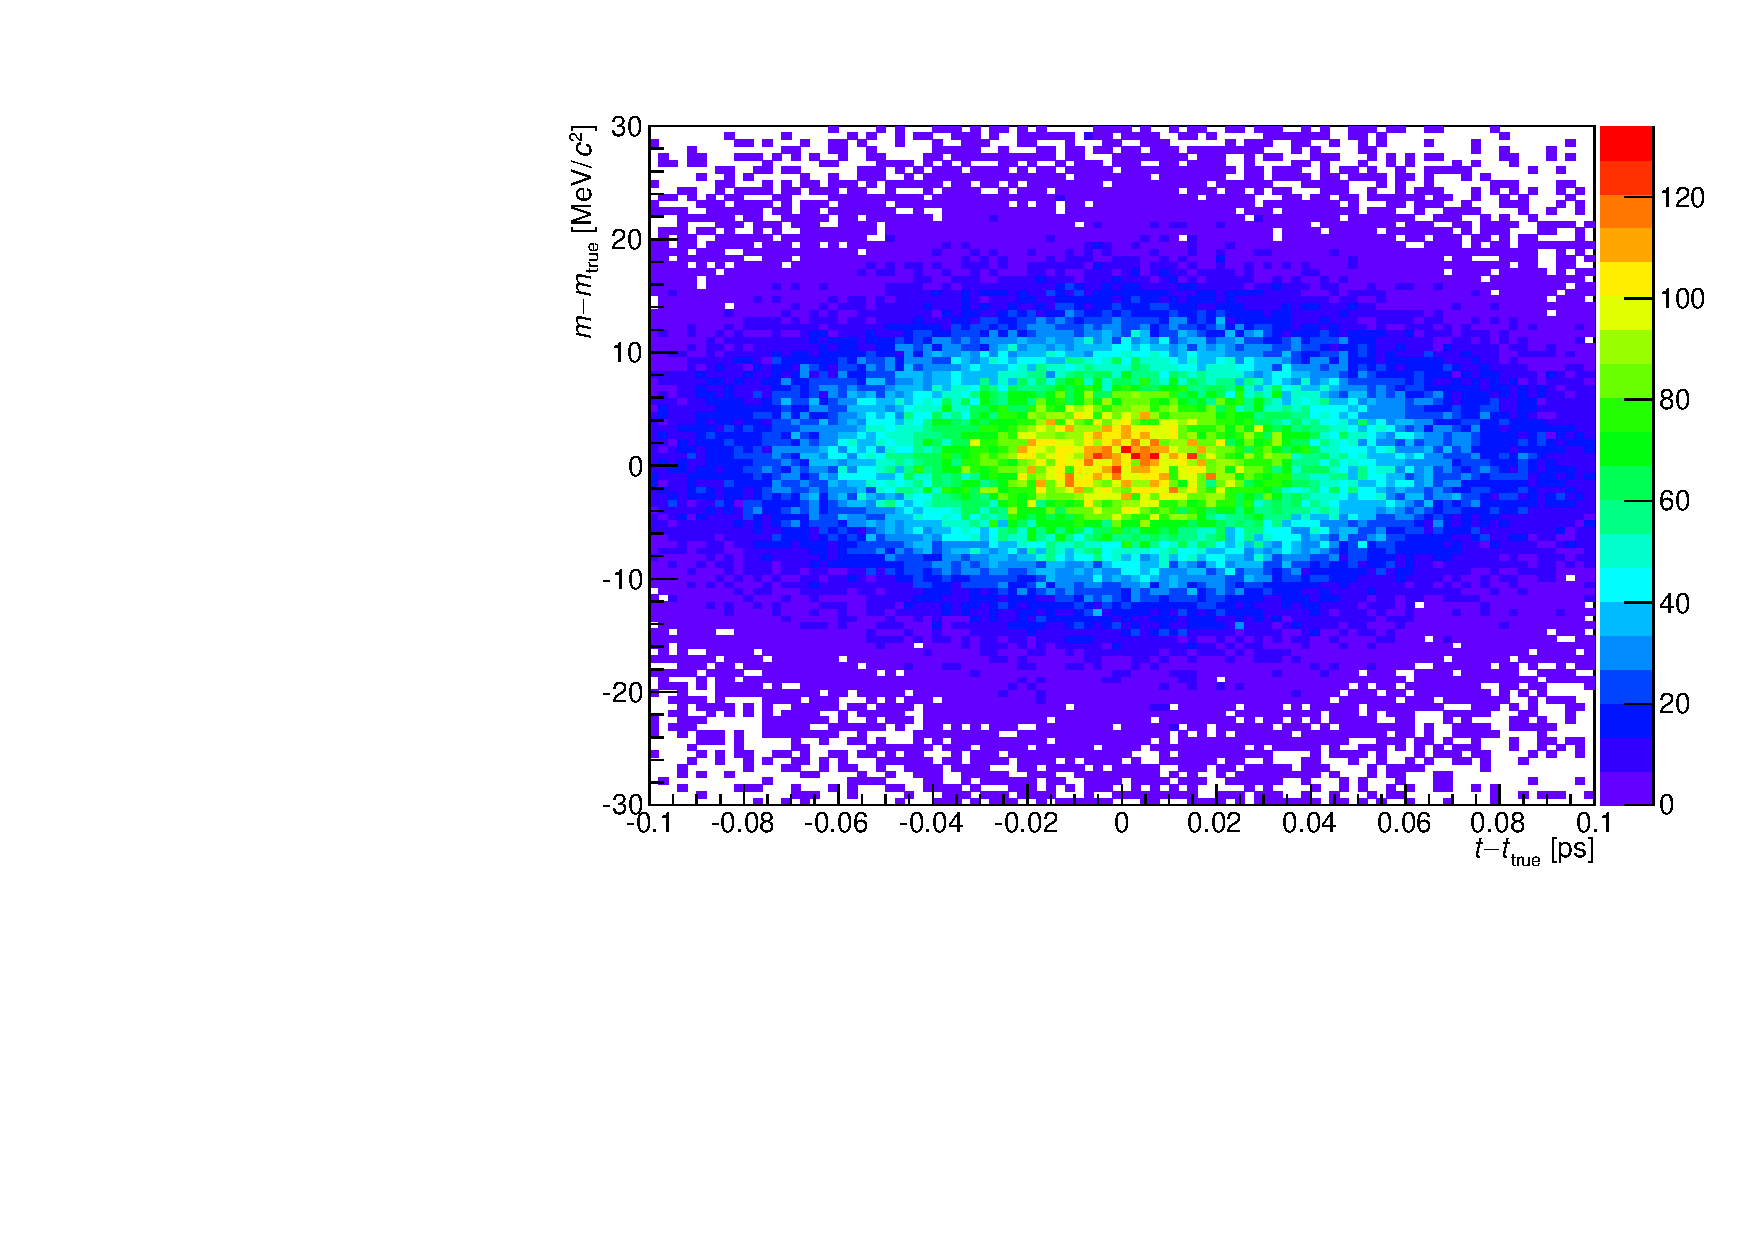
\includegraphics[width=0.49\textwidth]{private/content/measurement-of-sin2beta/figs/systematics_fitmodel_mtcorr_dd.pdf}\hfill
  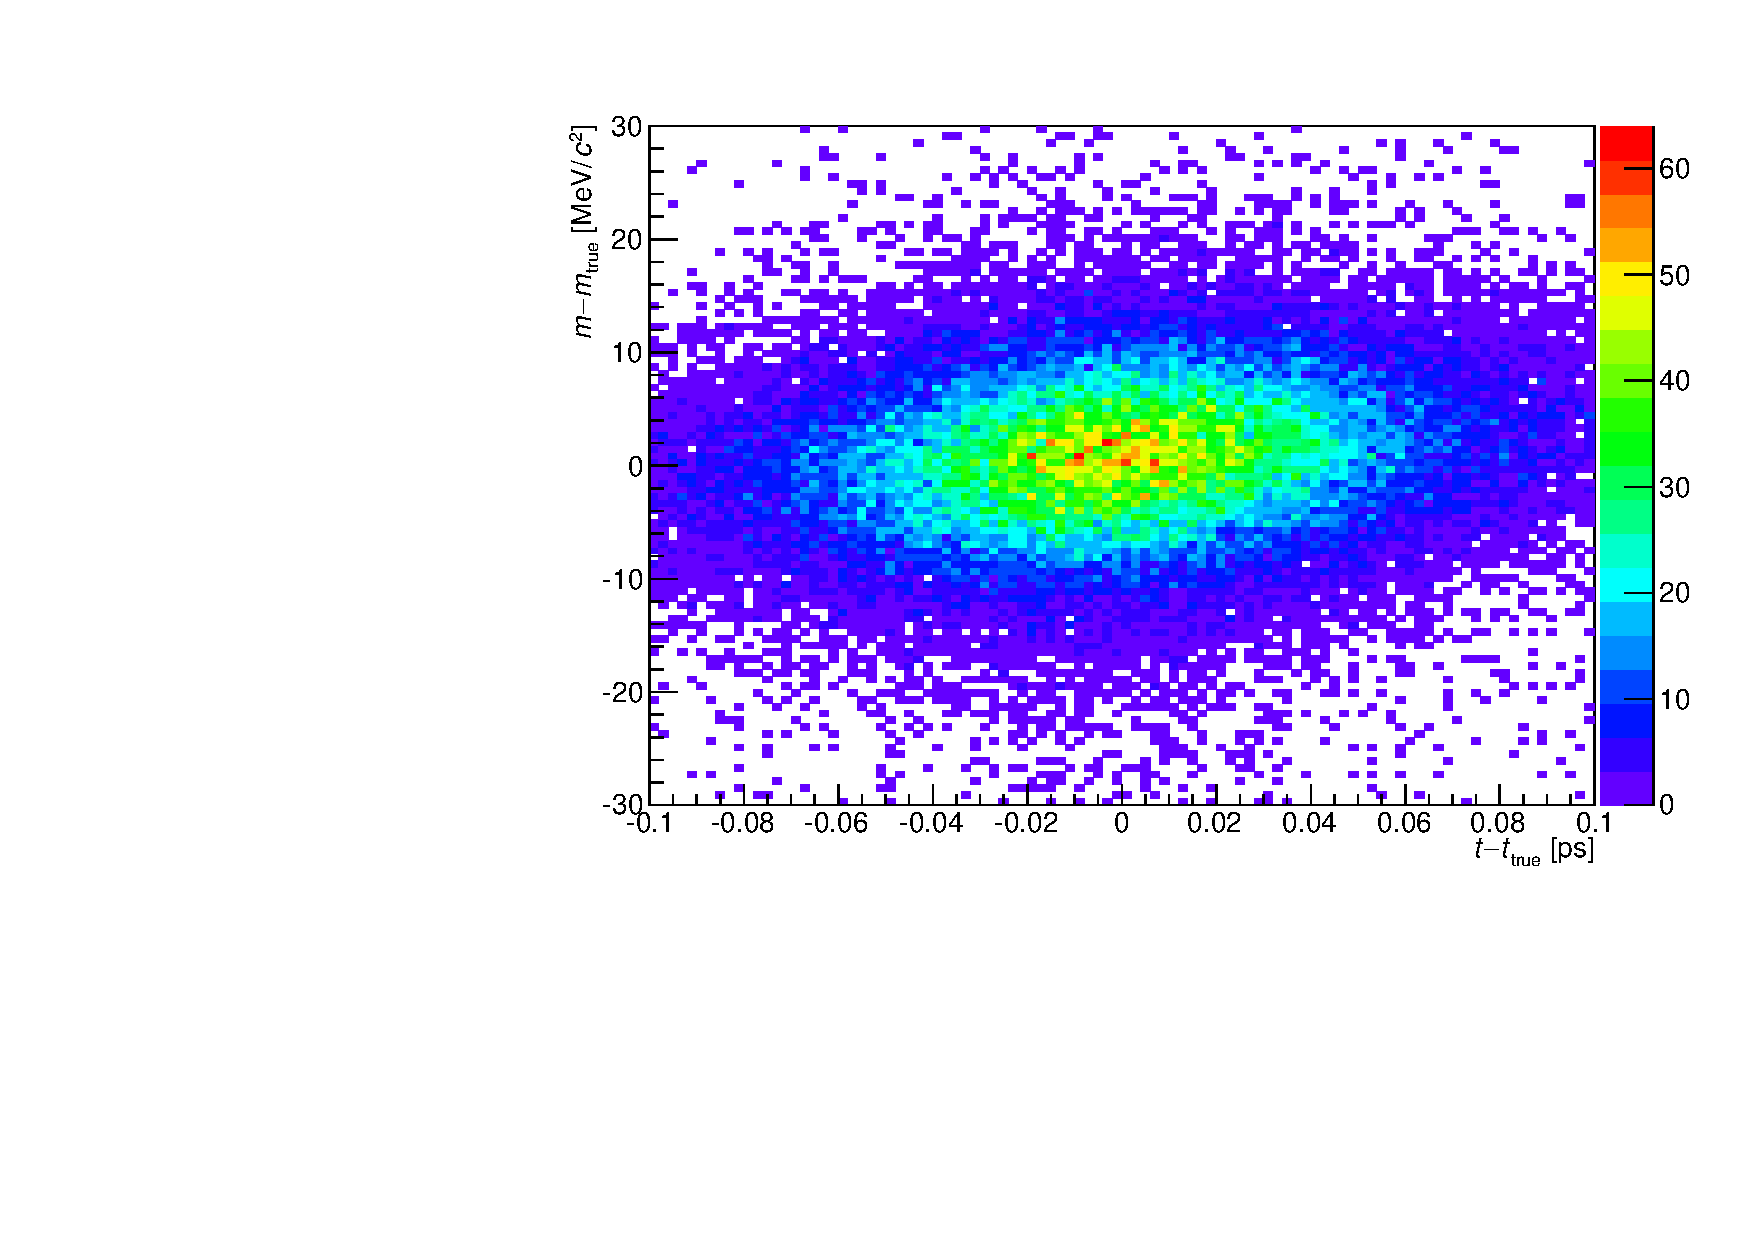
\includegraphics[width=0.49\textwidth]{private/content/measurement-of-sin2beta/figs/systematics_fitmodel_mtcorr_ll.pdf}
  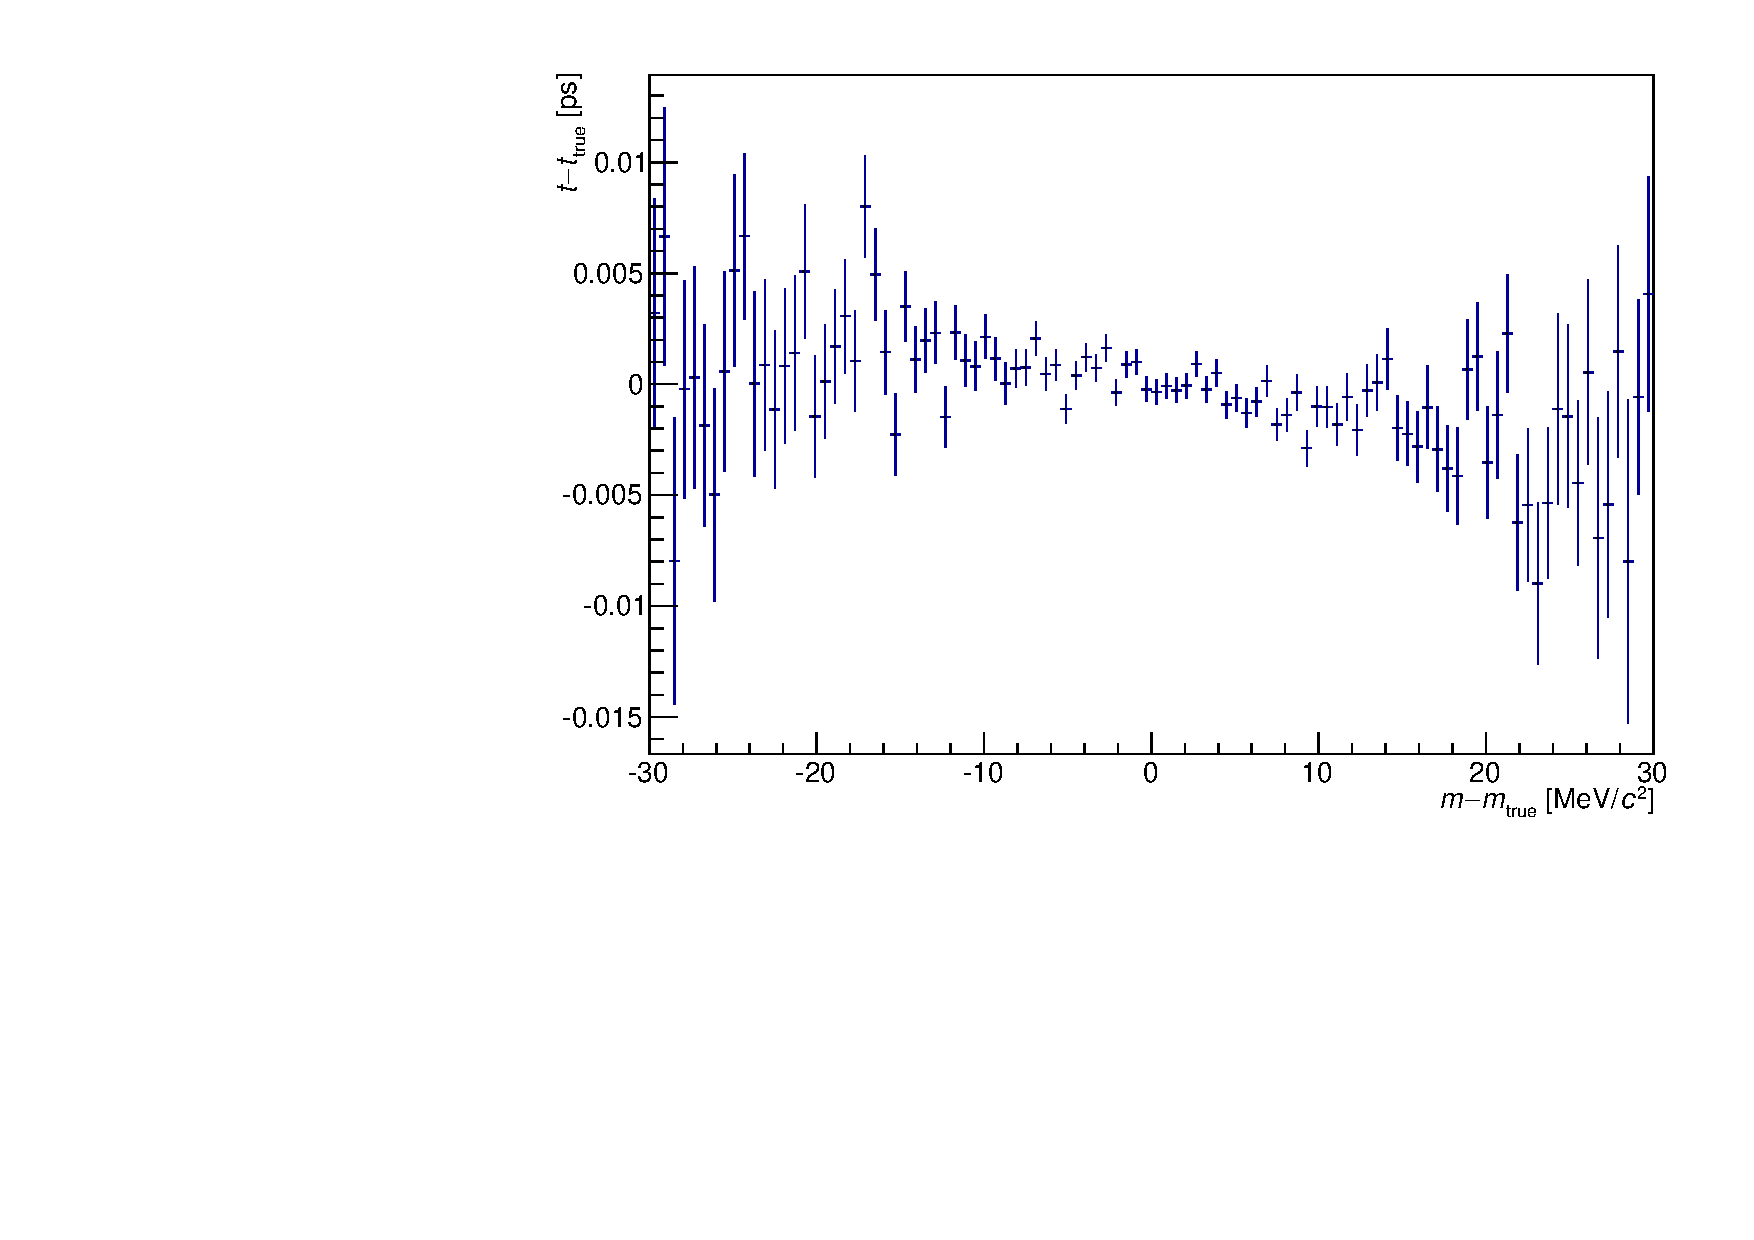
\includegraphics[width=0.49\textwidth]{private/content/measurement-of-sin2beta/figs/systematics_fitmodel_mtcorr_profile_dd.pdf}\hfill
  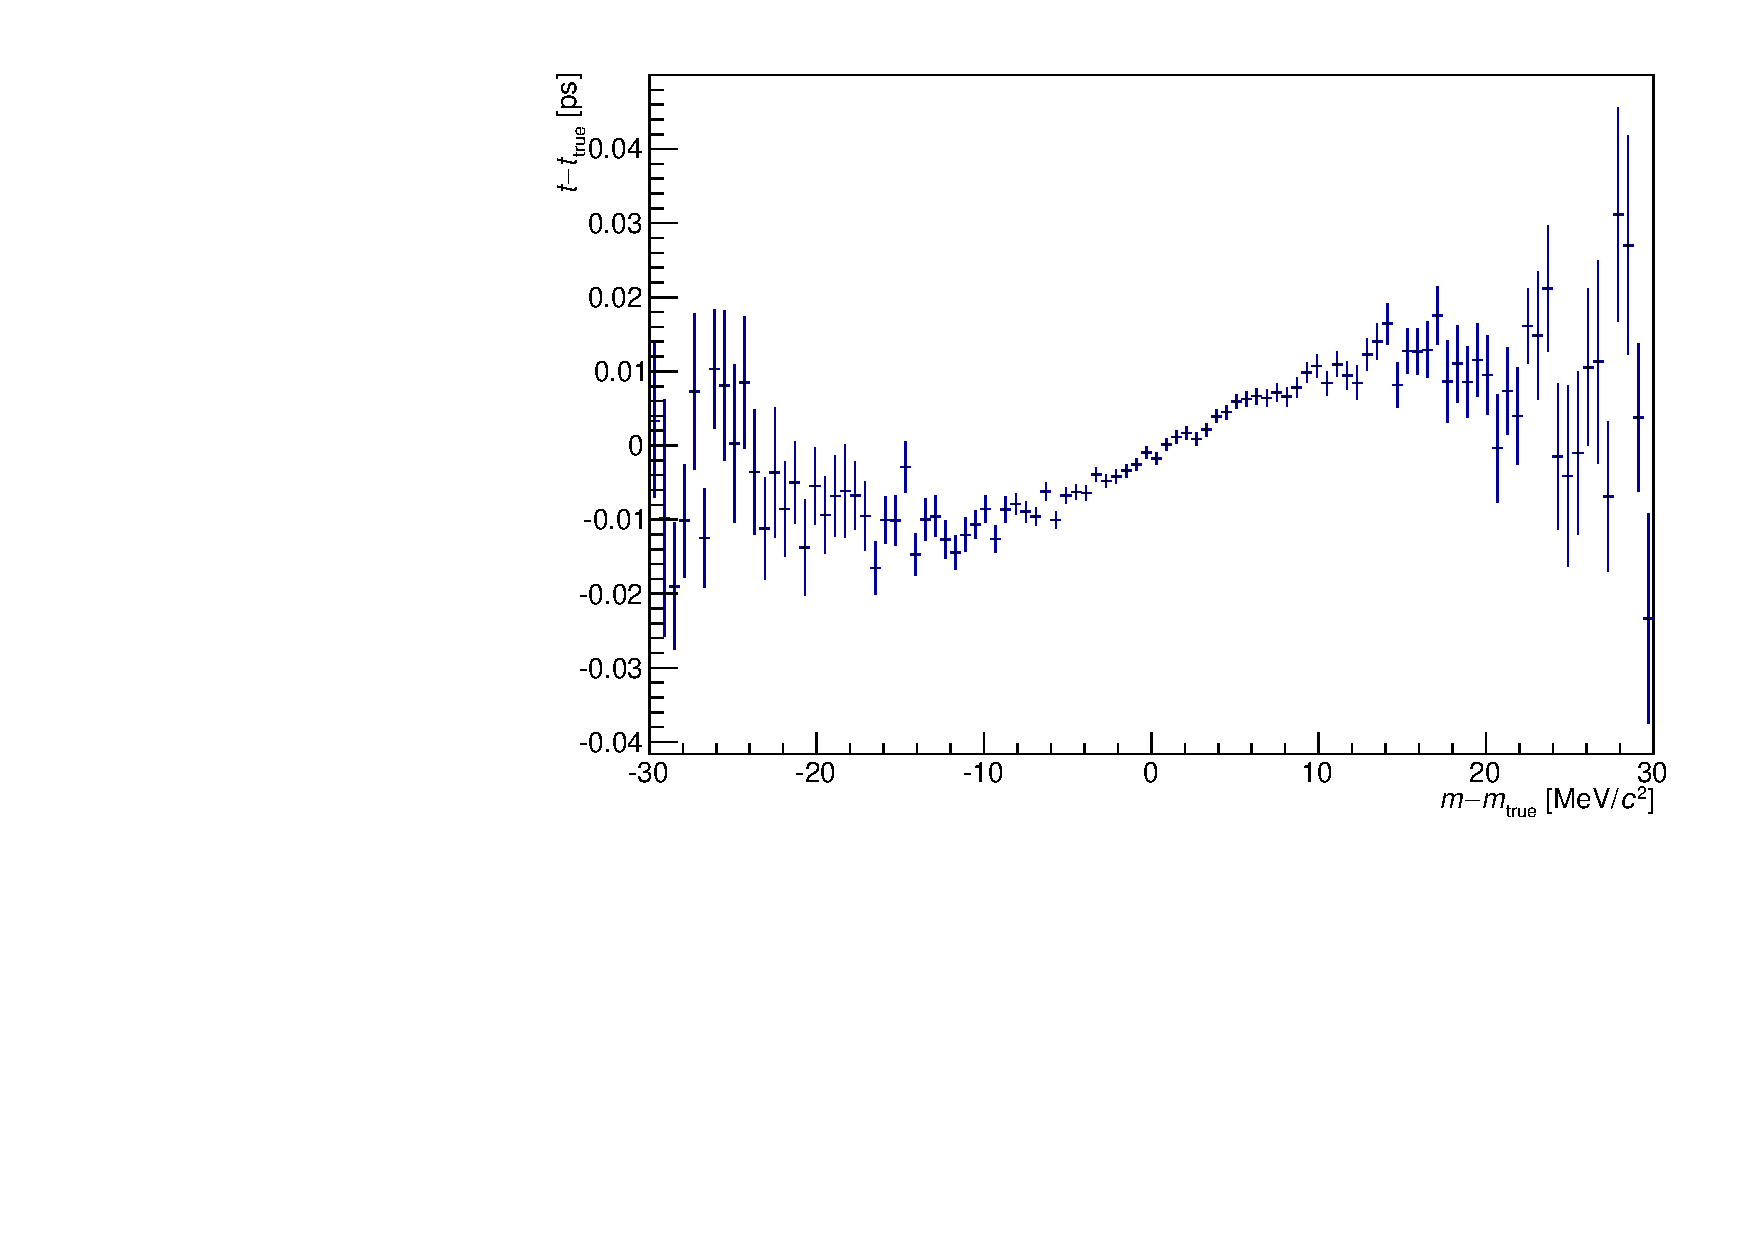
\includegraphics[width=0.49\textwidth]{private/content/measurement-of-sin2beta/figs/systematics_fitmodel_mtcorr_profile_ll.pdf}
\caption{Visualisation of the correlation between the mass and the decay time
resolution defined $m-m_\text{true}$ and $\obsTime-\obsTime_\text{true}$. On top
the binned 2-dimensional distribution is shown, while on the bottom profile
plots show the average of the decay time resolution as a function of the mass
resolution. Shown are the (left) \catDD and the (right) \catLL subsamples.}
\label{fit:measurement_of_sin2beta:systematics:systematics:fit_model:mass_time_correlations}
\end{figure}
%
In a study with $\num{250}$ iterations data are generated assuming the given
correlation for \catLL candidates while fitted with the nominal model. The pull
and residual plots shown in 
\cref{fig:app:measurement_of_sin2beta:systematics:systematics:fit_model:mass_time_correlations} 
show no significant bias on the \CP parameters.

%...............................................................................
\subsubsection{Flavour Tagging}
\label{sec:measurement_of_sin2beta:systematics:systematics:tagging}

The statistical uncertainties on the flavour tagging calibration parameters
($\p{0,1}{\text{\acs*{OS},\acs*{SSpi}}}$ and
$\deltap{0,1}{\text{\acs*{OS},\acs*{SSpi}}}$) are taken into account using
Gaussian constraints (\cf
\cref{sec:measurement_of_sin2beta:cpv_measurement:constrained_parameters}). The
influence of the systematic uncertainties are investigated by a \ToyMC study.

First, the eight parameters are varied up and down by one systematic uncertainty
and the effect on the effective dilution is studied. This reduces to $16$
combinations if varying $\p{i}{j}$ and $\deltap{i}{j}$ only in the same
direction. For each combination $\num{750}$ iterations are performed and the
dilution is calculated. The largest deviation is found when all $\p{0}{j}$
parameters are varied up and all $\p{1}{j}$ parameters are varied down. As the
dilution and the \CP parameters are part of a product in the \PDF the relative
change in dilution of $\SI{1.5}{\percent}$ is already an estimate of the
systematic uncertainty.

A \ToyMC study with $\num{1000}$ iterations is performed using values for the
\CP parameters drawn from a Gaussian distribution where the central value is
shifted according to the result of the preparatory study and the statistical
uncertainty is used as width while including all correlations of the calibration
parameters 
(\cf \cref{eq:flavour_tagging:calibration:os:parameters,tab:flavour_tagging:calibration:ss:correlations}).
The nominal model is used in the subsequent fit. As depicted in 
\cref{fig:app:measurement_of_sin2beta:systematics:systematics:tagging} a
significant bias is observed. The offsets of the residual distributions
%
\begin{equation}
  \delta_{\SJpsiKS} = \num{0.0062}\eqthinspace\text{and}\eqthinspace\delta_{\CJpsiKS} = \num{0.0024}
\end{equation}
%
are used as an estimate of the systematic uncertainties.

%...............................................................................
\subsubsection{Decay time resolution}
\label{sec:measurement_of_sin2beta:systematics:systematics:resolution}

\paragraph{In the calibration of the decay time estimate} a linear function is
used. In a \ToyMC study the influence of a different parametrisation of the
calibration model is investigated. Based on the results given in
\cref{sec:measurement_of_sin2beta:resolution_and_acceptance:resolution} a
parabolic function with non-zero (zero) offset is used in the \catDD
(\catLL) subsample to generate data, that is then fitted using the nominal
calibration model. The parameter values used in the generation are given in
\cref{tab:measurement_of_sin2beta:systematics:systematics:resolution:parabolic_parameters}.
In a study with $\num{1000}$ iterations no significant bias is found as can been
seen in the pull and residual distributions provided in
\cref{fig:app:measurement_of_sin2beta:systematics:systematics:resolution:calibration}.
%
\begin{table}[h]
\centering
\caption{Fit parameters of the parabolic decay time resolution calibration
function for \catDD and \catLL candidates. No offset parameter is used in case
of the \catLL model, thus the correspondent entries are marked with a dash.}
\label{tab:measurement_of_sin2beta:systematics:systematics:resolution:parabolic_parameters}
\sisetup{
  table-number-alignment    = center,
  table-sign-mantissa,
}
  \begin{tabular}{
    ll
    S[
      table-figures-integer     = 1,
      table-figures-decimal     = 4,
      table-figures-uncertainty = 4,
    ]
    S[
      table-figures-integer     = 1,
      table-figures-decimal     = 2,
      table-figures-uncertainty = 2,
    ]
  }
    \toprule
    \multicolumn{2}{c}{Parameter}               & {\catDD}          & {\catLL}      \\
    \midrule
    $a_{1}$         &   (\si{\per\pico\second}) & -1.7    +- 1.3    & -4.3  +- 0.7  \\
    $b_{1}$         &                           &  1.04   +- 0.014  &  1.33 +- 0.07 \\
    $c_{1}$         &   (\si{\pico\second})     &  0.0044 +- 0.0027 & {---}         \\
    $a_{2}$         &   (\si{\per\pico\second}) & -1.5    +- 3.4    & -2.5  +- 1.0  \\
    $b_{2}$         &                           &  1.5    +- 0.4    &  2.15 +- 0.27 \\
    $c_{2}$         &   (\si{\pico\second})     &  0.016  +- 0.008  & {---}         \\
    \bottomrule
  \end{tabular}
\end{table}

\paragraph{An offset to the central values} of the three Gaussian \acp{PDF} is
used in the parametrisation of the decay time resolution model (\cf
\cref{eq:measurement_of_sin2beta:resolution_and_acceptance:resolution}). Due to
technical limitations in the implementation of the cubic spline \acp{PDF} the
value of this offset $\mu_{\obsTime}$ has to be set to zero in the nominal fit
although non-zero values are found in the determination of the resolution model.
The influence of ignoring the non-zero values is tested in a \ToyMC study with
$\num{250}$ iterations, where the data is generated using the offset's value
originally determined, while fitting with the nominal fit model. No significant
bias is observed. Plots of the pull and residual distributions are shown in
\cref{fig:app:measurement_of_sin2beta:systematics:systematics:resolution:offset}.

\paragraph{The fraction of wrongly associated \acp{PV}} is assumed to be
independent of the decay time resolution estimate $\obsTimeError$. This ignores
an increase in the fraction $f_\text{\acs*{PV}}$ as a function of the decay time
error. The influence of this simplification is tested in a \ToyMC study with
$\num{1000}$ iterations, where the fraction varies following a parabolic
function with offset fixed to zero in the generation, while $f_\text{\acs*{PV}}$
is set as in the nominal model in the subsequent fit. As depicted in
\cref{fig:app:measurement_of_sin2beta:systematics:systematics:resolution:wrong_pv} 
a significant bias is present for the parameter $\SJpsiKS$ as well as for
$\CJpsiKS$. Thus, systematic uncertainties of
%
\begin{equation}
  \delta_{\SJpsiKS} = \num{0.0021}\eqthinspace\text{and}\eqthinspace\delta_{\CJpsiKS} = \num{0.0011}
\end{equation}
%
are assigned.

%...............................................................................
\subsubsection{Decay time acceptance}
\label{sec:measurement_of_sin2beta:systematics:systematics:acceptance}

\paragraph{The low decay time acceptance's} influence on the \CP parameters is
studied using a modified acceptance shape. In the generation histograms of the
time-dependent ratios $\varepsilon_{\catAU}$ and $\varepsilon_{\catEB}$ (\cf
\cref{sec:measurement_of_sin2beta:resolution_and_acceptance:acceptance:lower})
are employed that are determined on the signal \MC sample using the same
methodology as used for the nominal model. In $\num{250}$ iterations the
generated data are fitted using the nominal (\catOT and \catOS) fit model, as no
influence from the tagging decision and the year of data taking is expected. The
\ToyMC study shows no significant bias. Pull and residual distributions can be
found in
\cref{fig:app:measurement_of_sin2beta:systematics:systematics:acceptance:lower}.

\paragraph{The upper decay time acceptance} is parametrised in the nominal fit
using a linear scale model. As outlined in
\cref{sec:measurement_of_sin2beta:resolution_and_acceptance:acceptance:upper}
higher order effects are studied using a quadratic correction function but are
not considered in the fit later on. To estimate the impact of a deviating
correction function on the \CP parameters a \ToyMC study with $\num{1000}$
iterations is performed. As the upper decay time acceptance is not expected to
dependent on the trigger category nor the tagging category, data are only
generated using the (\catAU and \catOS) fit model. The generation is performed
using the parametrisation given in \cref{eq:measurement_of_sin2beta:resolution_and_acceptance:acceptance:upper:quadratic} 
with parameters fixed to the values shown in
\cref{tab:measurement_of_sin2beta:resolution_and_acceptance:acceptance:upper:quadratic}. 
In the fit the nominal model with a linear correction function is used. No
deviation of a standard normal distribution is found for the \SJpsiKS pull
distribution. A small bias on \CJpsiKS is visible in the pull distribution,
therefore a systematic uncertainty of
%
\begin{equation}
  \delta_{\CJpsiKS} = \num{0.0012}
\end{equation}
%
is assigned. Pull and residual distributions can be found in
\cref{fig:app:measurement_of_sin2beta:systematics:systematics:acceptance:upper}.

%...............................................................................
\subsubsection[Production asymmetry, $z$-scale, \DMd, and \DGd]{Production asymmetry, $\mathbfsfit{z}$-scale, $\mathbfsfit{\DMd}$, and $\mathbfsfit{\DGd}$}
\label{sec:measurement_of_sin2beta:systematics:systematics:further_studies}

\paragraph{The $\mathbfsfit{z}$-scale alignment} of the \LHCb detector is known
up to a relative uncertainty of $\sigma_\text{$z$-scale} =
\SI{0.022}{\percent}$. To study how this affects the measurement of the \CP
parameters, data are generated using an offset of $\mu_{t} =
\sigma_\text{$z$-scale} t$ in the decay time resolution model. In the fit the
offset is set to zero as in the nominal fit model. In a \ToyMC study with
$\num{1000}$ iterations a small bias is observed for \SJpsiKS as well as for
\CJpsiKS and systematic uncertainties of
%
\begin{equation}
  \delta_{\SJpsiKS} = \num{0.0012}\eqthinspace\text{and}\eqthinspace\delta_{\CJpsiKS} = \num{0.0023}
\end{equation}
%
are assigned. Pull and residual distributions can be found in
\cref{fig:app:measurement_of_sin2beta:systematics:systematics:further_studies:zscale}.

\paragraph{The influence of the production asymmetry} on the measurement of
\SJpsiKS and \CJpsiKS is investigated in a \ToyMC study. In $\num{1000}$
iterations, samples are produced with an enlarged production asymmetry and
subsequently fitted with the nominal fit model. The production asymmetry is
varied by one systematic uncertainty: $A_P^{\catOO} = \num{-0.0122}$ while
$\Delta A_P$ is not shifted, as any systematic effect from the difference of the
production asymmetry between \catOO and \catOT is already covered. No systematic
shift is observed. The pull and residual distributions are depicted in 
\cref{fig:app:measurement_of_sin2beta:systematics:systematics:further_studies:production_asymmetry}.

\paragraph{The \Bdbfsf decay width difference's} impact on the \CP measurement
is examined in a \ToyMC study with $\num{1000}$ iterations. The data is
generated using $\DGd = \SI{0.007}{\per\pico\second}$ as an upper approximation
based on the current world average of the ratio between the decay width
difference and the absolute decay width $\DGd/\Gd = \num{0.001 +- 0.010}$
\cite{Amhis:2014hma}. The fit then neglects the non-zero $\DGd$ value as in the
nominal model. A significant bias is observed in the pull distribution of
$\SJpsiKS$, thus a systematic uncertainty of
%
\begin{equation}
  \delta_{\SJpsiKS} = \num{0.0047}
\end{equation}
%
is assigned as an estimate to cover for this effect. The pull and residual
distributions for $\SJpsiKS$ and $\CJpsiKS$ are depicted in
\cref{fig:app:measurement_of_sin2beta:systematics:systematics:further_studies:decay_width_difference}.

\paragraph{The \Bdbfsf mass difference $\mathbfsfit{\DMd}$} is taken as a
constrained external input to the fit model. The influence of the systematic
uncertainty on $\DMd$ is treated in a \ToyMC study with $\num{1000}$ iterations
of generation and fit. In the generation the value of the mass difference is
enlarged by the systematic uncertainty, \ie $\DMd =
\SI{0.512}{\planckbar\per\pico\second}$, the nominal model is used in the fit.
The pull distribution of $\CJpsiKS$ shows a significant deviation, therefore the
offset of the residual distribution
%
\begin{equation}
  \delta_{\CJpsiKS} = \num{0.0034}
\end{equation}
%
is taken as an estimate of the systematic uncertainty.
\Cref{fig:app:measurement_of_sin2beta:systematics:systematics:further_studies:mass_difference} 
shows the pull and residual distributions for $\SJpsiKS$ and $\CJpsiKS$.

% ------------------------------------------------------------------------------
\subsection{Summary of systematic effects}
\label{sec:measurement_of_sin2beta:systematics:summary}

The systematic uncertainties are summarised in
\cref{tab:measurement_of_sin2beta:systematics:summary}. The overall systematic
uncertainty is calculated by summing the single uncertainties in quadrature. The
relative systematic uncertainties compared to the central values of $\SJpsiKS$
and $\CJpsiKS$ are given in brackets. Here, $\SJpsiKS = \num{0.729}$ and
$\CJpsiKS = \num{-0.033}$ are set as reference values.
%
\begin{table}[h]
  \caption{Systematic uncertainties $\delta_{\SJpsiKS}$ and $\delta_{\CJpsiKS}$
  on $\SJpsiKS$ and $\CJpsiKS$. Entries marked with a dash represent studies
  where no significant effect is observed.}
  \label{tab:measurement_of_sin2beta:systematics:summary}
  \begin{tabular}{lrlrl}
    \toprule
    Origin & \multicolumn{2}{c}{$\delta_{\SJpsiKS}$} & \multicolumn{2}{c}{$\delta_{\CJpsiKS}$}    \\
    \midrule
    {Background tagging asymmetry}           &  $\tablenum[table-format = 1.4]{0.0179}$ & ($\tablenum[table-format = 1.1]{2.5}\si{\percent}$) &  $\tablenum[table-format = 1.4]{0.0015}$ & ($\tablenum[table-format = 2.1]{4.5}\si{\percent}$) \\
    {Tagging calibration}                    &  $\tablenum[table-format = 1.4]{0.0062}$ & ($\tablenum[table-format = 1.1]{0.9}\si{\percent}$) &  $\tablenum[table-format = 1.4]{0.0024}$ & ($\tablenum[table-format = 2.1]{7.2}\si{\percent}$) \\
    {$\DGd$}                                 &  $\tablenum[table-format = 1.4]{0.0047}$ & ($\tablenum[table-format = 1.1]{0.6}\si{\percent}$) &  \multicolumn{2}{c}{---}               \\
    {Fraction of wrong PV component}         &  $\tablenum[table-format = 1.4]{0.0021}$ & ($\tablenum[table-format = 1.1]{0.3}\si{\percent}$) &  $\tablenum[table-format = 1.4]{0.0011}$ & ($\tablenum[table-format = 2.1]{3.3}\si{\percent}$) \\
    {$z$-scale}                              &  $\tablenum[table-format = 1.4]{0.0012}$ & ($\tablenum[table-format = 1.1]{0.2}\si{\percent}$) &  $\tablenum[table-format = 1.4]{0.0023}$ & ($\tablenum[table-format = 2.1]{7.0}\si{\percent}$) \\
    {$\DMd$}                                 &  \multicolumn{2}{c}{---}               &  $\tablenum[table-format = 1.4]{0.0034}$ & ($\tablenum[table-format = 2.1]{10.3}\si{\percent}$)\\
    {Upper decay time acceptance}            &  \multicolumn{2}{c}{---}               &  $\tablenum[table-format = 1.4]{0.0012}$ & ($\tablenum[table-format = 2.1]{3.6}\si{\percent}$) \\
    {Correlation between mass and decay time}&  \multicolumn{2}{c}{---}               &  \multicolumn{2}{c}{---}               \\
    {Decay time resolution calibration}      &  \multicolumn{2}{c}{---}               &  \multicolumn{2}{c}{---}               \\
    {Decay time resolution offset}           &  \multicolumn{2}{c}{---}               &  \multicolumn{2}{c}{---}               \\
    {Low decay time acceptance}              &  \multicolumn{2}{c}{---}               &  \multicolumn{2}{c}{---}               \\
    {Production asymmetry}                   &  \multicolumn{2}{c}{---}               &  \multicolumn{2}{c}{---}               \\
    \midrule
    Sum                                            &  $0.020$        & ($\tablenum[table-format = 1.1]{2.7}\si{\percent}$) & $0.005$          & ($\tablenum[table-format = 2.1]{15.2}\si{\percent}$)\\
    \bottomrule
  \end{tabular}
\end{table}

